%&pdfLaTeX
% !TEX encoding = UTF-8 Unicode
\documentclass[a4paper]{article}
\usepackage{ifxetex}
\ifxetex
\usepackage{fontspec}
\setmainfont[Mapping=tex-text]{STIXGeneral}
\else
\usepackage[T1]{fontenc}
\usepackage[latin1]{inputenc}
\fi
\usepackage{textcomp}

\usepackage{graphicx}
\usepackage{array}
\usepackage{fixltx2e}
\usepackage{amssymb}
\usepackage{fancyhdr}
\usepackage{amsmath}
\usepackage{algpseudocode}
\usepackage{threeparttable}
\usepackage{tikz}
\usetikzlibrary{positioning,shapes.multipart}
\usetikzlibrary{decorations.pathreplacing}
\renewcommand{\headrulewidth}{0pt}
\renewcommand{\footrulewidth}{0pt}

\newcommand\bits{\,\mbox{bits}}
\newcommand\MB{\,\mbox{MB}}

\setlength{\parindent}{0cm}
\setlength{\parskip}{0.18cm}
\usepackage[hmargin=2cm,vmargin=2.5cm,bindingoffset=0.0cm]{geometry}
\usepackage[pdfborder={0 0 0}]{hyperref}
\begin{document}



%&pdfLaTeX
% !TEX encoding = UTF-8 Unicode
\documentclass[a4paper]{article}
\usepackage{ifxetex}
\ifxetex
\usepackage{fontspec}
\setmainfont[Mapping=tex-text]{STIXGeneral}
\else
\usepackage[T1]{fontenc}
\usepackage[latin1]{inputenc}
\fi
\usepackage{textcomp}

\usepackage{graphicx}
\usepackage{array}
\usepackage{fixltx2e}
\usepackage{amssymb}
\usepackage{fancyhdr}
\usepackage{amsmath}
\usepackage{algpseudocode}
\usepackage{threeparttable}
\usepackage{tikz}
\usetikzlibrary{positioning,shapes.multipart}
\usetikzlibrary{decorations.pathreplacing}
\renewcommand{\headrulewidth}{0pt}
\renewcommand{\footrulewidth}{0pt}

\newcommand\bits{\,\mbox{bits}}
\newcommand\MB{\,\mbox{MB}}

\setlength{\parindent}{0cm}
\setlength{\parskip}{0.18cm}
\usepackage[hmargin=2cm,vmargin=2.5cm,bindingoffset=0.0cm]{geometry}
\usepackage[pdfborder={0 0 0}]{hyperref}
\begin{document}



%&pdfLaTeX
% !TEX encoding = UTF-8 Unicode
\documentclass[a4paper]{article}
\usepackage{ifxetex}
\ifxetex
\usepackage{fontspec}
\setmainfont[Mapping=tex-text]{STIXGeneral}
\else
\usepackage[T1]{fontenc}
\usepackage[latin1]{inputenc}
\fi
\usepackage{textcomp}

\usepackage{graphicx}
\usepackage{array}
\usepackage{fixltx2e}
\usepackage{amssymb}
\usepackage{fancyhdr}
\usepackage{amsmath}
\usepackage{algpseudocode}
\usepackage{threeparttable}
\usepackage{tikz}
\usetikzlibrary{positioning,shapes.multipart}
\usetikzlibrary{decorations.pathreplacing}
\renewcommand{\headrulewidth}{0pt}
\renewcommand{\footrulewidth}{0pt}

\newcommand\bits{\,\mbox{bits}}
\newcommand\MB{\,\mbox{MB}}

\setlength{\parindent}{0cm}
\setlength{\parskip}{0.18cm}
\usepackage[hmargin=2cm,vmargin=2.5cm,bindingoffset=0.0cm]{geometry}
\usepackage[pdfborder={0 0 0}]{hyperref}
\begin{document}



%&pdfLaTeX
% !TEX encoding = UTF-8 Unicode
\documentclass[a4paper]{article}
\usepackage{ifxetex}
\ifxetex
\usepackage{fontspec}
\setmainfont[Mapping=tex-text]{STIXGeneral}
\else
\usepackage[T1]{fontenc}
\usepackage[latin1]{inputenc}
\fi
\usepackage{textcomp}

\usepackage{graphicx}
\usepackage{array}
\usepackage{fixltx2e}
\usepackage{amssymb}
\usepackage{fancyhdr}
\usepackage{amsmath}
\usepackage{algpseudocode}
\usepackage{threeparttable}
\usepackage{tikz}
\usetikzlibrary{positioning,shapes.multipart}
\usetikzlibrary{decorations.pathreplacing}
\renewcommand{\headrulewidth}{0pt}
\renewcommand{\footrulewidth}{0pt}

\newcommand\bits{\,\mbox{bits}}
\newcommand\MB{\,\mbox{MB}}

\setlength{\parindent}{0cm}
\setlength{\parskip}{0.18cm}
\usepackage[hmargin=2cm,vmargin=2.5cm,bindingoffset=0.0cm]{geometry}
\usepackage[pdfborder={0 0 0}]{hyperref}
\begin{document}



\input{CRAMv3.ver}
\title{CRAM format specification (version 3.1)}
\author{samtools-devel@lists.sourceforge.net}
\date{\headdate}
\maketitle


\begin{quote}\small
The master version of this document can be found at
\url{https://github.com/samtools/hts-specs}.\\
This printing is version~\commitdesc\ from that repository,
last modified on the date shown above.
\end{quote}

\begin{center}
\textit{license: Apache 2.0}
\end{center}
\vspace*{1em}

\section{\textbf{Overview}}

This specification describes the CRAM 3.0 and 3.1 formats.

CRAM has the following major objectives:

\begin{enumerate}
\item Significantly better lossless compression than BAM

\item Full compatibility with BAM

\item Effortless transition to CRAM from using BAM files

\item Support for controlled loss of BAM data
\end{enumerate}

The first three objectives allow users to take immediate advantage of the CRAM 
format while offering a smooth transition path from using BAM files. The fourth 
objective supports the exploration of different lossy compression strategies and 
provides a framework in which to effect these choices. Please note that the CRAM 
format does not impose any rules about what data should or should not be preserved. 
Instead, CRAM supports a wide range of lossless and lossy data preservation strategies 
enabling users to choose which data should be preserved.

Data in CRAM is stored either as CRAM records or using one of the general purpose 
compressors (gzip, bzip2). CRAM records are compressed using a number of different 
encoding strategies. For example, bases are reference compressed by encoding base
differences rather than storing the bases themselves.\footnote{Markus Hsi-Yang Fritz,
Rasko Leinonen, Guy Cochrane, and Ewan Birney,
\textbf{Efficient storage of high throughput DNA sequencing data using reference-based compression},
{\sl Genome Res.}~2011~21: 734--740;
\href{http://dx.doi.org/doi:10.1101/gr.114819.110}{doi:10.1101/gr.114819.110};
{\sc pmid:}21245279.}

\section{\textbf{Data types}}

CRAM specification uses logical data types and storage data types; logical data 
types are written as words (e.g. int) while physical data types are written using 
single letters (e.g. i). The difference between the two is that storage data types 
define how logical data types are stored in CRAM. Data in CRAM is stored either 
as bits or bytes. Writing values as bits and bytes is described in detail 
below.

\subsection{\textbf{Logical data types}}

\begin{description}
\item[Byte]\ \newline
Signed byte (8 bits).

\item[Integer]\ \newline
Signed 32-bit integer. 

\item[Long]\ \newline
Signed 64-bit integer. 

\item[Array]\ \newline
An array of any logical data type: array\texttt{<}type\texttt{>}
\end{description}

% \begin{tabular}{ll}
% \textbf{Byte}    & Signed byte (8 bits).  \\
% \\
% \textbf{Integer} & Signed 32-bit integer. \\
% \\
% \textbf{Long}    & Signed 64-bit integer. \\
% \\
% \textbf{Array}   & An array of any logical data type: \texttt{<}type\texttt{>}[ ] \\
% \end{tabular}

\subsection{\textbf{Writing bits to a bit stream}}

A bit stream consists of a sequence of 1s and 0s. The bits are written most significant 
bit first where new bits are stacked to the right and full bytes on the left are 
written out. In a bit stream the last byte will be incomplete if less than 8 bits 
have been written to it. In this case the bits in the last byte are shifted to 
the left.

\subsubsection*{Example of writing to bit stream}

Let's consider the following example. The table below shows a sequence of write 
operations: 

\begin{tabular}{|l|l|l|l|l|}
\hline
\textbf{Operation order} & \textbf{Buffer state before} & \textbf{Written bits} & \textbf{Buffer state after} & \textbf{Issued bytes}\tabularnewline
\hline
1 & 0x0 & 1 & 0x1 & -\tabularnewline
\hline
2 & 0x1 & 0 & 0x2 & -\tabularnewline
\hline
3 & 0x2 & 11 & 0xB & -\tabularnewline
\hline
4 & 0xB & 0000 0111 & 0x7 & 0xB0\tabularnewline
\hline
\end{tabular}

After flushing the above bit stream the following bytes are written: 0xB0 0x70. 
Please note that the last byte was 0x7 before shifting to the left and became 0x70 
after that:

\texttt{> echo "obase=16; ibase=2; 00000111" \textbar{} bc\\
7\\
\\
> echo "obase=16; ibase=2; 01110000" \textbar{} bc\\
70}

And the whole bit sequence: 

\texttt{> echo "obase=2; ibase=16; B070" \textbar{} bc\\
1011000001110000}

When reading the bits from the bit sequence it must be known that only 12 bits 
are meaningful and the bit stream should not be read after that. 

\subsubsection*{Note on writing to bit stream}

When writing to a bit stream both the value and the number of bits in the value 
must be known. This is because programming languages normally operate with bytes 
(8 bits) and to specify which bits are to be written requires a bit-holder, for 
example an integer, and the number of bits in it. Equally, when reading a value 
from a bit stream the number of bits must be known in advance. In case of prefix 
codes (e.g. Huffman) all possible bit combinations are either known in advance 
or it is possible to calculate how many bits will follow based on the first few 
bits. Alternatively, two codes can be combined, where the first contains the number 
of bits to read. 

\subsection{\textbf{Writing bytes to a byte stream}}
\label{subsec:writing-bytes}

The interpretation of byte stream is straightforward. CRAM uses \emph{little endianness}
for bytes when applicable and defines the following storage data types:

\begin{description}

\item[Boolean (bool)]\ \newline
Boolean is written as 1-byte with 0x0 being `false' and 0x1 being `true'.

\item[Integer (int32)]\ \newline
Signed 32-bit integer, written as 4 bytes in little-endian byte order.

\item[Long (int64)]\ \newline
Signed 64-bit integer, written as 8 bytes in little-endian byte order.

\item[ITF-8 integer (itf8)]\ \newline
This is an alternative way to write an integer value. The idea is similar to UTF-8 
encoding and therefore this encoding is called ITF-8 (Integer Transformation Format 
- 8 bit). 

The most significant bits of the first byte have special meaning and are called 
`prefix'. These are 0 to 4 true bits followed by a 0. The number of 1's denote 
the number of bytes to follow. To accommodate 32 bits such representation requires 
5 bytes with only 4 lower bits used in the last byte 5.

\item[LTF-8 long (ltf8)]\ \newline
See ITF-8 for more details. The only difference between ITF-8 and LTF-8 is the 
number of bytes used to encode a single value. To do so 64 bits are required and 
this can be done with 9 byte at most with the first byte consisting of just 1s 
or 0xFF value. 

\item[{Array (array\texttt{<}type\texttt{>})}]\ \newline
A variable sized array with an explicitly written dimension.
Array length is written first as integer (itf8), followed by the elements of the array.

Implicit or fixed-size arrays are also used, written as \textit{type}\texttt{[ ]} or \textit{type}\texttt{[4]} (for example).
These have no explicit dimension included in the file format and instead rely on the specification itself to document the array size.


\item[{Encoding}]\ \newline
Encoding is a data type that specifies how data series have been compressed. Encodings 
are defined as encoding\texttt{<}type\texttt{>} where the type is a logical data 
type as opposed to a storage data type.

An encoding is written as follows. The first integer (itf8) denotes the codec id 
and the second integer (itf8) the number of bytes in the following encoding-specific 
values. 

Subexponential encoding example: 

\begin{tabular}{|l|l|l|}
\hline
\textbf{Value} & \textbf{Type} & \textbf{Name}\tabularnewline
\hline
0x7 & itf8 & codec id\tabularnewline
\hline
0x2 & itf8 & number of bytes to follow\tabularnewline
\hline
0x0 & itf8 & offset\tabularnewline
\hline
0x1 & itf8 & K parameter\tabularnewline
\hline
\end{tabular}

The first byte ``0x7'' is the codec id. 

The next byte ``0x2'' denotes the length of the bytes to follow (2). 

The subexponential encoding has 2 parameters: integer (itf8) offset and integer (itf8) K.

offset = 0x0 = 0

K = 0x1 = 1


\item[{Map}]\ \newline
A map is a collection of keys and associated values. A map with N keys is written 
as follows: 

\begin{tabular}{|l|l|l|l|l|l|l|l|}
\hline
size in bytes & N & key 1 & value 1 & key ... & value ... & key N & value N\tabularnewline
\hline
\end{tabular}

Both the size in bytes and the number of keys are written as integer (itf8). Keys 
and values are written according to their data types and are specific to each map.

\item[String]\ \newline
A string is represented as byte arrays using UTF-8 format. Read names, reference 
sequence names and tag values with type `Z' are stored as UTF-8.

\end{description}


\section{\textbf{Encodings }}

Encoding is a data structure that captures information about compression details 
of a data series that are required to uncompress it. This could be a set of constants 
required to initialize a specific decompression algorithm or statistical properties 
of a data series or, in case of data series being stored in an external block, 
the block content id. 

Encoding notation is defined as the keyword `encoding' followed by its data type 
in angular brackets, for example `encoding\texttt{<}byte\texttt{>}' stands for 
an encoding that operates on a data series of data type `byte'. 

Encodings may have parameters of different data types, for example the EXTERNAL 
encoding has only one parameter, integer id of the external block. The following 
encodings are defined: 

\begin{tabular}{|l|l|>{\raggedright}p{155pt}|>{\raggedright}p{160pt}|}
\hline
\textbf{Codec} & \textbf{ID} & \textbf{Parameters} & \textbf{Comment}\tabularnewline
\hline
NULL & 0 & none & series not preserved\tabularnewline
\hline
EXTERNAL & 1 & int block content id & the block content identifier used to associate 
external data blocks with data series\tabularnewline
\hline
Deprecated (GOLOMB) & 2 & int offset, int M & Golomb coding\tabularnewline
\hline
HUFFMAN & 3 & array\texttt{<}int\texttt{>}, array\texttt{<}int\texttt{>} & coding with int/byte values\tabularnewline
\hline
BYTE\_ARRAY\_LEN & 4 & encoding\texttt{<}int\texttt{>} array length, encoding\texttt{<}byte\texttt{>} 
bytes & coding of byte arrays with array length\tabularnewline
\hline
BYTE\_ARRAY\_STOP & 5 & byte stop, int external block\linebreak{}
content id & coding of byte arrays with a stop value \tabularnewline
\hline
BETA & 6 & int offset, int number of bits & binary coding\tabularnewline
\hline
SUBEXP & 7 & int offset, int K & subexponential coding\tabularnewline
\hline
Deprecated (GOLOMB\_RICE) & 8 & int offset, int log$_{\text{2}}$m & Golomb-Rice coding\tabularnewline
\hline
GAMMA & 9 & int offset & Elias gamma coding\tabularnewline
\hline
\end{tabular}

See section~\ref{sec:encodings} for more detailed descriptions of all the above coding algorithms and their parameters.

\section{\textbf{Checksums}}
The checksumming is used to ensure data integrity. The following checksumming algorithms are used in CRAM.
\subsection{\textbf{CRC32}}
This is a cyclic redundancy checksum 32-bit long with the polynomial 0x04C11DB7. Please refer to \href{http://www.itu.int/rec/recommendation.asp?type=folders&lang=e&parent=T-REC-V.42}{ITU-T V.42} for more details. The value of the CRC32 hash function is written as an integer.
\subsection{\textbf{CRC32 sum}}
CRC32 sum is a combination of CRC32 values by summing up all individual CRC32 values modulo 2\textsuperscript{32}. 

\section{\textbf{File structure}}

The overall CRAM file structure is described in this section. Please refer to other 
sections of this document for more detailed information. 

A CRAM file consists of a fixed length file definition, followed by a CRAM header container,
then zero or more data containers, and finally a special end-of-file container.

\begin{center}
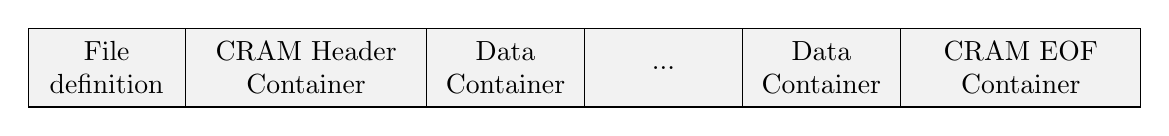
\begin{tikzpicture}[
  every node/.style={scale=1.0},
  boxes/.style={rectangle split,rectangle split parts=#1,draw,rectangle split horizontal,text width=5em,align=center,minimum height=1cm,fill=black!5,on grid},
  notes/.style={text width=20em,align=center,minimum height=1cm,on grid},
]
\node (file) [boxes=6] {
\nodepart{one}File definition
\nodepart[text width=8em]{two}CRAM Header Container
\nodepart{three}Data Container
\nodepart{four}...
\nodepart{five}Data Container
\nodepart[text width=8em]{six}CRAM EOF Container
};
\end{tikzpicture}

Figure 1: A CRAM file consists of a file definition, followed by a header container, then other containers.
\end{center}

Containers consist of one or more blocks. The first container, called the CRAM header container,
is used to store a textual header as described in the SAM specification (see the section 7.1).

\begin{center}
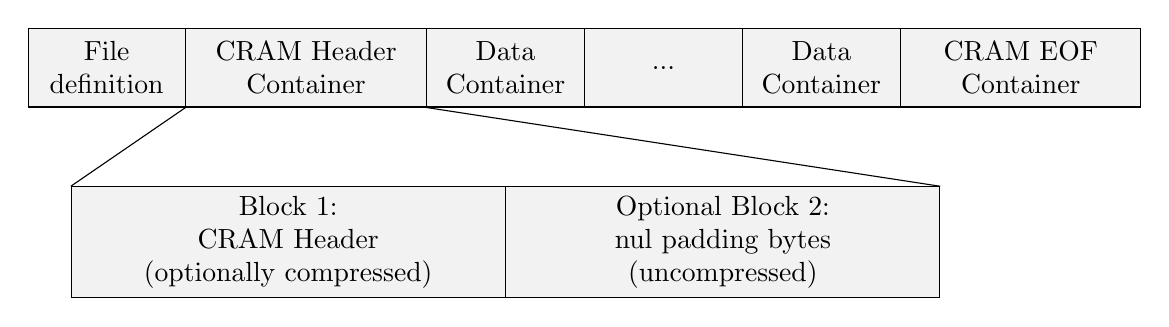
\begin{tikzpicture}[
  every node/.style={scale=1.0},
  boxes/.style={rectangle split,rectangle split parts=#1,draw,rectangle split horizontal,text width=5em,align=center,minimum height=1cm,fill=black!5,on grid},
  notes/.style={text width=20em,align=center,minimum height=1cm,on grid},
]
\node (file) [boxes=6] {
\nodepart{one}File definition
\nodepart[text width=8em]{two}CRAM Header Container
\nodepart{three}Data Container
\nodepart{four}...
\nodepart{five}Data Container
\nodepart[text width=8em]{six}CRAM EOF Container
};

\node (header) [boxes=2,below=1 of file.three south, text width=15em] {
\nodepart{one}Block 1:\break
CRAM Header\break
(optionally compressed)
\nodepart{two}Optional Block 2:\break
nul padding bytes\break
(uncompressed)
};
\draw (file.one split south) to (header.north west);
\draw (file.two split south) to (header.north east);
\end{tikzpicture}

Figure 2: The the first container holds the CRAM header text.
\end{center}

Each container starts with a container header structure followed by
one or more blocks.
The first block in each container is the compression header block
giving details of how to decode data in subsequent blocks.
Each block starts with a block header structure followed by the block
data.

\begin{center}
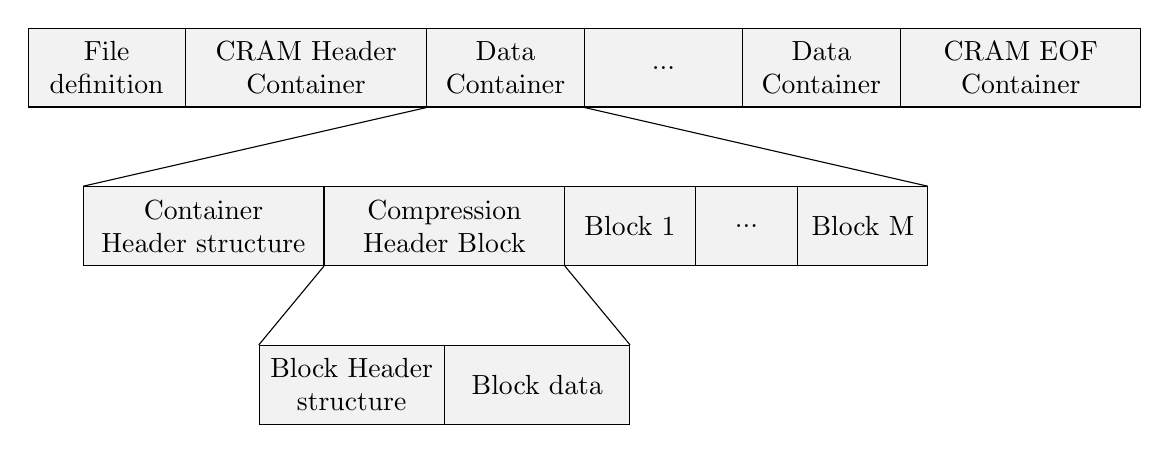
\begin{tikzpicture}[
  every node/.style={scale=1.0},
  boxes/.style={rectangle split,rectangle split parts=#1,draw,rectangle split horizontal,text width=5em,align=center,minimum height=1cm,fill=black!5,on grid},
  notes/.style={text width=20em,align=center,minimum height=1cm,on grid},
]
\node (file) [boxes=6] {
\nodepart{one}File definition
\nodepart[text width=8em]{two}CRAM Header Container
\nodepart{three}Data Container
\nodepart{four}...
\nodepart{five}Data Container
\nodepart[text width=8em]{six}CRAM EOF Container
};

\node (container) [boxes=5,below=1 of file.three south,text width=8em] {
\nodepart{one}Container Header structure
\nodepart{two}Compression Header Block
\nodepart[text width=4em]{three}Block 1
\nodepart[text width=3em]{four}...
\nodepart[text width=4em]{five}Block M
};
\draw (file.two split south) to (container.north west);
\draw (file.three split south) to (container.north east);

\node (blocks) [boxes=2,below=1 of container.two south,text width=6em] {
\nodepart{one}Block Header structure
\nodepart{two}Block data
};
\draw (container.one split south) to (blocks.north west);
\draw (container.two split south) to (blocks.north east);
\end{tikzpicture}

Figure 3: Containers as a series of blocks
\end{center}

The blocks after the compression header are organised logically into slices. One 
slice may contain, for example, a contiguous region of alignment data. Slices begin 
with a slice header block and are followed by one or more data blocks.
It is these data blocks which hold the primary bulk of CRAM data.
The data blocks are further subdivided into a core data block and one or more external data blocks.

\begin{center}
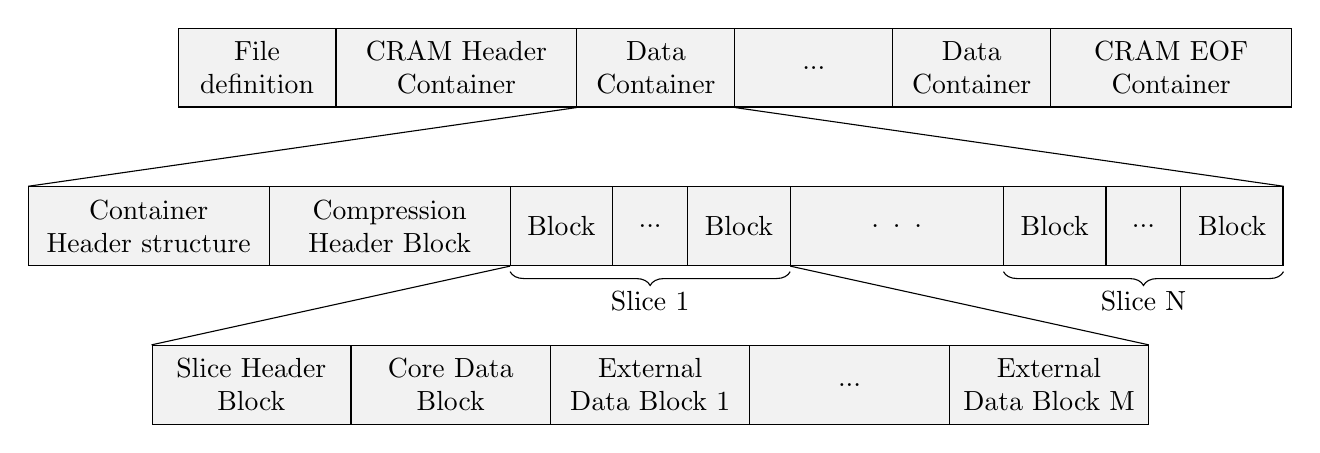
\begin{tikzpicture}[
  every node/.style={scale=1.0},
  boxes/.style={rectangle split,rectangle split parts=#1,draw,rectangle split horizontal,text width=5em,align=center,minimum height=1cm,fill=black!5,on grid},
  notes/.style={text width=20em,align=center,minimum height=1cm,on grid},
]
\node (file) [boxes=6] {
\nodepart{one}File definition
\nodepart[text width=8em]{two}CRAM Header Container
\nodepart{three}Data Container
\nodepart{four}...
\nodepart{five}Data Container
\nodepart[text width=8em]{six}CRAM EOF Container
};

\node (container) [boxes=9,below=1 of file.three south,text width=8em] {
\nodepart{one}Container Header structure
\nodepart{two}Compression Header Block
\nodepart[text width=3em]{three}Block
\nodepart[text width=2em]{four}...
\nodepart[text width=3em]{five}Block
\nodepart[text width=7em]{six}. . .
\nodepart[text width=3em]{seven}Block
\nodepart[text width=2em]{eight}...
\nodepart[text width=3em]{nine}Block
};
\draw (file.two split south) to (container.north west);
\draw (file.three split south) to (container.north east);

\draw[decoration={brace,mirror,amplitude=5pt,raise=2pt},decorate]
  (container.two split south) to (container.five split south);
\node [below=0.2 of container.four south] {Slice 1};

\draw[decoration={brace,mirror,amplitude=5pt,raise=2pt},decorate]
  (container.six split south) to (container.south east);
\node [below=0.2 of container.eight south] {Slice N};

\node (slice) [boxes=5,below=1 of container.four south, text width=6.5em] {
\nodepart{one}Slice Header Block
\nodepart{two}Core Data Block
\nodepart{three}External Data Block 1
\nodepart{four}...
\nodepart{five}External Data Block M
};
\draw (container.two split south) to (slice.north west);
\draw (container.five split south) to (slice.north east);
\end{tikzpicture}

Figure 4: Slices formed from a series of concatenated blocks
\end{center}

\section{\textbf{File definition}}

Each CRAM file starts with a fixed length (26 bytes) definition with the following 
fields:

\begin{tabular}{|l|l|l|}
\hline
\textbf{Data type} & \textbf{Name} & \textbf{Value}\tabularnewline
\hline
byte[4] & format magic number & CRAM (0x43 0x52 0x41 0x4d)\tabularnewline
\hline
unsigned byte & major format number & 3 (0x3)\tabularnewline
\hline
unsigned byte & minor format number & 1 (0x1)\tabularnewline
\hline
byte[20] & file id & CRAM file identifier (e.g. file name or SHA1 checksum)\tabularnewline
\hline
\end{tabular}

Valid CRAM \textit{major}.\textit{minor} version numbers are as follows:

\begin{itemize}
\item[\textit{1.0}]
The original public CRAM release.

\item[\textit{2.0}]
The first CRAM release implemented in both Java and C; tidied up
implementation vs specification differences in \textit{1.0}.

\item[\textit{2.1}]
Gained end of file markers; compatible with \textit{2.0}.

\item[\textit{3.0}]
Additional compression methods; header and data checksums;
improvements for unsorted data.

\item[\textit{3.1}]
Additional EXTERNAL compression codecs only.
\end {itemize}

CRAM 3.0 and 3.1 differ only in the list of compression
methods available, so tools that output CRAM 3 without using any 3.1
codecs should write the header to indicate 3.0 in order to permit
maximum compatibility.

\section{\textbf{Container header structure}}
\label{sec:container}

The file definition is followed by one or more containers with the following header 
structure where the container content is stored in the `blocks' field:

\begin{tabular}{|l|>{\raggedright}p{120pt}|>{\raggedright}p{260pt}|}
\hline
\textbf{Data type} & \textbf{Name} & \textbf{Value}
\tabularnewline
\hline
int32 & length & the sum of the lengths of all blocks in this container (headers and data); 
equal to the total byte length of the container minus the byte length of this header structure\tabularnewline
\hline
itf8 & reference sequence id & reference sequence identifier  or\linebreak{}
-1 for unmapped reads\linebreak{}
-2 for multiple reference sequences.\linebreak{}
All slices in this container must have a reference sequence id matching this value.\tabularnewline
\hline
itf8 & starting position on the reference & the alignment start position\tabularnewline
\hline
itf8 & alignment span & the length of the alignment\tabularnewline
\hline
itf8 & number of records & number of records in the container\tabularnewline
\hline
ltf8 & record counter & 1-based sequential index of records in the file/stream.\tabularnewline
\hline
ltf8 & bases & number of read bases\tabularnewline
\hline
itf8 & number of blocks & the total number of blocks in this container\tabularnewline
\hline
array\texttt{<}itf8\texttt{>} & landmarks & the locations of slices in this container as byte offsets from the end of
this container header, used for random access indexing.
For sequence data containers, the landmark count must equal the slice count.\linebreak{}
Since the block before the first slice is the compression header,
landmarks[0] is equal to the byte length of the compression header.\tabularnewline
\hline
int & crc32 & CRC32 hash of the all the preceding bytes in the container.\tabularnewline
\hline
byte[ ] & blocks & The blocks contained within the container.\tabularnewline
\hline
\end{tabular}

In the initial CRAM header container, the reference sequence id,
starting position on the reference, and alignment span fields must be
ignored when reading. The landmarks array is optional for the CRAM
header, but if it exists it should point to block offsets instead of
slices, with the first block containing the textual header.

In data containers specifying unmapped reads or multiple reference
sequences (i.e. reference sequence id $< 0$), the starting position on
the reference and alignment span fields must be ignored when
reading. When writing, it is recommended to set each of these ignored
fields to the value 0.


\subsection{\textbf{CRAM header container}}
\label{subsec:cram-header-container}

The first container in a CRAM file contains a textual header in one or more blocks.  See section~\ref{subsec:header-block} for more details on the layout of data within these blocks and constraints applied to the contents of the SAM header.

The landmarks field of the container header structure may be used to
indicate the offsets of the blocks used in the header container.
These may optionally be omitted by specifying an array size of zero.

\section{\textbf{Block structure}}
\label{sec:block-struct}

Containers consist of one or more blocks. Block compression is applied independently 
and in addition to any encodings used to compress data within the block. The block 
have the following header structure with the data stored in the `block data' field:

\begin{tabular}{|l|>{\raggedright}p{120pt}|>{\raggedright}p{260pt}|}
\hline
\textbf{Data type} & \textbf{Name} & \textbf{Value}
\tabularnewline
\hline
byte & method & the block compression method (and first CRAM version): \linebreak{}
0: raw (none)*\linebreak{}
1: gzip\linebreak{}
2: bzip2 (v2.0)\linebreak{}
3: lzma (v3.0)\linebreak{}
4: rans4x8 (v3.0)\linebreak{}
5: rans4x16 (v3.1)\linebreak{}
6: adaptive arithmetic coder (v3.1)\linebreak{}
7: fqzcomp (v3.1)\linebreak{}
8: name tokeniser (v3.1)
\tabularnewline
\hline
byte & block content type id & the block content type identifier\tabularnewline
\hline
itf8 & block content id & the block content identifier used to associate external 
data blocks with data series\tabularnewline
\hline
itf8 & size in bytes* & size of the block data after applying block compression\tabularnewline
\hline
itf8 & raw size in bytes* & size of the block data before applying block compression\tabularnewline
\hline
byte[ ] & block data & the data stored in the block:\linebreak{}
$\bullet$ bit stream of CRAM records (core data block)\linebreak{}
$\bullet$ byte stream (external data block)\linebreak{}
$\bullet$ additional fields ( header blocks)\tabularnewline
\hline
byte[4] & CRC32 & CRC32 hash value for all preceding bytes in the block\tabularnewline
\hline
\end{tabular}

* Note on raw method: both compressed and raw sizes must be set to the same value.

Empty blocks may occur in the files.
Blocks with a raw (uncompressed) size of zero are treated as empty,
irrespective of their ``method'' byte.  This is equivalent to
interpreting them as having method zero (raw) and compressed size of
zero.

\subsection{\textbf{Block content types}}

CRAM has the following block content types:

\begin{threeparttable}[t]
\begin{tabular}{|>{\raggedright}p{143pt}|>{\raggedright}p{45pt}|>{\raggedright}p{116pt}|>{\raggedright}p{114pt}|}
\hline
\textbf{Block content type} & \textbf{Block content type id} & \textbf{Name} & \textbf{Contents}\tabularnewline
\hline
FILE\_HEADER & 0 & CRAM header block & CRAM header\tabularnewline
\hline
COMPRESSION\_HEADER & 1 & Compression header block & See specific section\tabularnewline
\hline
SLICE\_HEADER\tnote{a} & 2 & Slice header block & See specific section\tabularnewline
\hline
 & 3 &  & reserved\tabularnewline
\hline
EXTERNAL\_DATA & 4 & external data block & data produced by external encodings\tabularnewline
\hline
CORE\_DATA & 5 & core data block & bit stream of all encodings except for external encodings\tabularnewline
\hline
\end{tabular}
\begin{tablenotes}
\item[a] Formerly MAPPED\_SLICE\_HEADER.  Now used by all slice headers regardless of mapping status.
\end{tablenotes}
\end{threeparttable}

\subsection{\textbf{Block content id}}

Block content id is used to distinguish between external blocks in the same slice. 
Each external encoding has an id parameter which must be one of the external block 
content ids. For external blocks the content id is a positive integer. For all 
other blocks content id should be 0. Consequently, all external encodings must 
not use content id less than 1. 

\subsubsection*{Data blocks}

Data is stored in data blocks. There are two types of data blocks: core data blocks 
and external data blocks.The difference between core and external data blocks is 
that core data blocks consist of data series that are compressed using bit encodings 
while the external data blocks are byte compressed. One core data block and any 
number of external data blocks are associated with each slice.

Writing to and reading from core and external data blocks is organised through 
CRAM records. Each data series is associated with an encoding. In case of external 
encodings the block content id is used to identify the block where the data series 
is stored. Please note that external blocks can have multiple data series associated 
with them; in this case the values from these data series will be interleaved. 


\subsection{\textbf{CRAM header block(s)}}
\label{subsec:header-block}

The SAM header is stored in the first block of the CRAM header container (see section~\ref{subsec:cram-header-container}).
This block may be uncompressed or gzip compressed only.
This block is followed by zero or more uncompressed expansion blocks.
If present, these permit in-place editing of the CRAM header, allowing it to grow or shrink with a compensatory size change applied to the subsequence expansion block, avoiding the need to rewrite the remainder of the file.
The contents of any expansion blocks should be zero bytes (nul characters).

The format of the initial SAM header block is a 32-bit little-endian integer holding the length of the text of the SAM header, minus nul-termination bytes, followed by the text itself.
Although 32-bit, the maximum permitted value is $2^{31}$, and all lengths must be positive.

The following constraints apply to the SAM header text: 

\begin{itemize}
\item The SQ:MD5 checksum is required unless the reference sequence has been embedded 
into the file.
\end{itemize}

\subsection{\textbf{Compression header block}}
\label{subsec:compression-header}

The compression header block consists of 3 parts: preservation map, data series 
encoding map and tag encoding map.

\subsubsection*{Preservation map}

The preservation map contains information about which data was preserved in the 
CRAM file. It is stored as a map with byte[2] keys:

\begin{tabular}{|l|l|>{\raggedright}p{100pt}|>{\raggedright}p{220pt}|}
\hline
\textbf{Key} & \textbf{Value data type} & \textbf{Name} & \textbf{Value}\tabularnewline
\hline
RN & bool & read names included & true if read names are preserved for all reads\tabularnewline
\hline
AP & bool & AP data series delta & true if AP data series is delta, false otherwise\tabularnewline
\hline
RR & bool & reference required & true if reference sequence is required to restore 
the data completely\tabularnewline
\hline
SM & byte[5] & substitution matrix & substitution matrix\tabularnewline
\hline
TD & array\texttt{<}byte\texttt{>} & tag ids dictionary & a list of lists of tag ids, see tag encoding section\tabularnewline
\hline
\end{tabular}

The boolean values are optional, defaulting to true when absent, although it is recommended to explicitly set them.  SM and TD are mandatory.

\subsubsection*{Data series encodings}

Each data series has an encoding. These encoding are stored in a map with byte[2] 
keys and are decoded in approximately this order\footnote{The precise order is defined in section~\ref{sec:record}.}:

\begin{threeparttable}[t]
\begin{tabular}{|l|l|>{\raggedright}p{100pt}|>{\raggedright}p{220pt}|}
\hline
\textbf{Key} & \textbf{Value data type} & \textbf{Name} & \textbf{Value}\tabularnewline
\hline
BF & encoding\texttt{<}int\texttt{>} & BAM bit flags & see separate section\tabularnewline
\hline
CF & encoding\texttt{<}int\texttt{>} & CRAM bit flags & see specific section\tabularnewline
\hline
RI & encoding\texttt{<}int\texttt{>} & reference id & record reference id from
the SAM file header\tabularnewline
\hline
RL & encoding\texttt{<}int\texttt{>} & read lengths & read lengths\tabularnewline
\hline
AP & encoding\texttt{<}int\texttt{>} & in-seq positions & if \textbf{AP-Delta} = true: 0-based alignment start
delta from the AP value in the previous record.
Note this delta may be negative, for example when switching references in a multi-reference slice.
When the record is the first in the slice, the previous position used is the slice alignment-start field (hence the first delta should be zero for single-reference slices, or the AP value itself for multi-reference slices).  \linebreak{}
if \textbf{AP-Delta} = false: encodes the alignment start position directly\tabularnewline
\hline
RG & encoding\texttt{<}int\texttt{>} & read groups & read groups. Special value 
`-1' stands for no group.\tabularnewline
\hline
RN\tnote{a} & encoding\texttt{<}byte[ ]\texttt{>} & read names & read names\tabularnewline
\hline
MF & encoding\texttt{<}int\texttt{>} & next mate bit flags & see specific section\tabularnewline
\hline
NS & encoding\texttt{<}int\texttt{>} & next fragment reference sequence id & reference 
sequence ids for the next fragment \tabularnewline
\hline
NP & encoding\texttt{<}int\texttt{>} & next mate alignment start & alignment positions 
for the next fragment\tabularnewline
\hline
TS & encoding\texttt{<}int\texttt{>} & template size & template sizes\tabularnewline
\hline
NF & encoding\texttt{<}int\texttt{>} & distance to next fragment & number of records
to skip to the next fragment\tnote{b}\tabularnewline
\hline
TL\tnote{c} & encoding\texttt{<}int\texttt{>} & tag ids  & list of tag ids, see tag encoding
section\tabularnewline
\hline
FN & encoding\texttt{<}int\texttt{>} & number of read features & number of read
features in each record\tabularnewline
\hline
FC & encoding\texttt{<}byte\texttt{>} & read features codes & see separate section\tabularnewline
\hline
FP & encoding\texttt{<}int\texttt{>} & in-read positions & positions of the read
features\tabularnewline
\hline
DL & encoding\texttt{<}int\texttt{>} & deletion lengths & base-pair deletion lengths\tabularnewline
\hline
BB & encoding\texttt{<}byte[ ]\texttt{>} & stretches of bases & bases\tabularnewline
\hline
QQ & encoding\texttt{<}byte[ ]\texttt{>} & stretches of quality scores & quality scores\tabularnewline
\hline
BS & encoding\texttt{<}byte\texttt{>} & base substitution codes & base substitution
codes\tabularnewline
\hline
IN & encoding\texttt{<}byte[ ]\texttt{>} & insertion & inserted bases\tabularnewline
\hline
RS & encoding\texttt{<}int\texttt{>} & reference skip length & number of skipped 
bases for the `N' read feature\tabularnewline
\hline
PD & encoding\texttt{<}int\texttt{>} & padding & number of padded bases\tabularnewline
\hline
HC & encoding\texttt{<}int\texttt{>} & hard clip & number of hard clipped bases\tabularnewline
\hline
SC & encoding\texttt{<}byte[ ]\texttt{>} & soft clip & soft clipped bases\tabularnewline
\hline
MQ & encoding\texttt{<}int\texttt{>} & mapping qualities & mapping quality scores\tabularnewline
\hline
BA & encoding\texttt{<}byte\texttt{>} & bases & bases\tabularnewline
\hline
QS & encoding\texttt{<}byte\texttt{>} & quality scores & quality scores\tabularnewline
\hline
TC\tnote{d} & N/A & legacy field & to be ignored\tabularnewline
\hline
TN\tnote{d} & N/A & legacy field & to be ignored\tabularnewline
\end{tabular}

\begin{tablenotes}
\item[a] Note RN this is decoded after MF if the record is detached from the mate and we are attempting to auto-generate read names.
\item[b] The count is reset for each slice so NF can only refer to a record later within this slice.
\item[c] TL is followed by decoding the tag values themselves, in order of appearance in the tag dictionary.
\item[d] TC and TN are legacy data series from CRAM 1.0.
They have no function in CRAM 3.0 and should not be present.
However some implementations do output them and decoders must silently skip these fields.
It is illegal for TC and TN to contain any data values, although there
may be empty blocks associated with them.
\end{tablenotes}
\end{threeparttable}

\subsubsection*{Tag encodings}
\label{subsubsec:tags}

The tag dictionary (TD) describes the unique combinations of tag id / type that occur on each alignment record.
For example if we search the id / types present in each record and find only two combinations -- X1:i BC:Z SA:Z: and X1:i: BC:Z -- then we have two dictionary entries in the TD map.

Let $L_{i}=\{T_{i0}, T_{i1}, \ldots, T_{ix}\}$ be a list of all tag ids for a record $R_{i}$, where $i$ is the sequential record index and $T_{ij}$ denotes $j$-th tag id in the record.
The list of unique $L_{i}$ is stored as the TD value in the preservation map.
Maintaining the order is not a requirement for encoders (hence ``combinations''), but it is permissible and thus different permutations, each encoded with their own elements in TD, should be supported by the decoder.
Each $L_{i}$ element in TD is assigned a sequential integer number starting with 0.
These integer numbers are referred to by the TL data series.
Using TD, an integer from the TL data series can be mapped back into a list of tag ids.
Thus per alignment record we only need to store tag values and not their ids and types.

The TD is written as a byte array consisting of $L_{i}$ values separated with \textbackslash{}0.
Each $L_{i}$ value is written as a concatenation of 3 byte $T_{ij}$ elements: tag id followed by BAM tag type code (one of A, c, C, s, S, i, I, f, F, Z, H or B, as described in the SAM specification).
For example the TD for tag lists X1:i BC:Z SA:Z and X1:i BC:Z may be encoded as X1CBCZSAZ\textbackslash{}0X1CBCZ\textbackslash{}0, with X1C indicating a 1 byte unsigned value for tag X1.

\subsubsection*{Tag values}

The encodings used for different tags are stored in a map.
The key is 3 bytes formed from the BAM tag id and type code, matching the TD dictionary described above.
Unlike the Data Series Encoding Map, the key is stored in the map as an ITF8 encoded integer, constructed using $(char1<<16) + (char2<<8) + type$.
For example, the 3-byte representation of OQ:Z is \{0x4F, 0x51, 0x5A\} and these bytes are interpreted as the integer key 0x004F515A, leading to an ITF8 byte stream \{0xE0, 0x4F, 0x51, 0x5A\}.

\begin{tabular}{|l|l|l|>{\raggedright}p{160pt}|}
\hline
\textbf{Key} & \textbf{Value data type} & \textbf{Name} & \textbf{Value}
\tabularnewline
\hline
TAG ID 1:TAG TYPE 1 & encoding\texttt{<}byte[ ]\texttt{>} & read tag 1 & tag values
(names and types are available in the data series code)\tabularnewline
\hline
... &  & ... & ...\tabularnewline
\hline
TAG ID N:TAG TYPE N & encoding\texttt{<}byte[ ]\texttt{>} & read tag N & ...\tabularnewline
\hline
\end{tabular}

Note that tag values are encoded as array of bytes. The routines to convert tag 
values into byte array and back are the same as in BAM with the exception of value 
type being captured in the tag key rather in the value.
Hence consuming 1 byte for types `C' and `c', 2 bytes for types `S' and `s', 4 bytes for types `I', `i' and `f', and a variable number of bytes for types `H', `Z' and `B'.

\subsection{\textbf{Slice header block}}

The slice header block is never compressed (block method=raw). For reference mapped 
reads the slice header also defines the reference sequence context of the data 
blocks associated with the slice. Mapped reads can be stored along with
\textbf{placed unmapped}\footnote{Unmapped reads can be \textit{placed} or \textit{unplaced}.
By placed unmapped read we mean a read that is unmapped according to bit 0x4 of the
BF (BAM bit flags) data series, but has position fields filled in, thus "placing"  it on a reference sequence. In contrast,
unplaced unmapped reads have have a reference sequence ID of -1 and alignment position of 0.}
reads on the same reference within the same slice.

Slices with the Multiple Reference flag (-2) set as the sequence ID in the header may contain reads
mapped to multiple external references, including unmapped\footnotemark[\value{footnote}] reads (placed on these references or unplaced),
but multiple embedded references cannot be combined in this way.  When multiple references are
used, the RI data series will be used to determine the reference sequence ID for each record.  This
data series is not present when only a single reference is used within a slice.

The Unmapped (-1) sequence ID in the header is for slices containing only unplaced
unmapped\footnotemark[\value{footnote}] reads.

A slice containing data that does not use the external reference in
any sequence may set the reference MD5 sum to zero.  This can happen
because the data is unmapped or the sequence has been stored verbatim
instead of via reference-differencing.  This latter scenario is
recommended for unsorted or non-coordinate-sorted data.

The slice header block contains the following fields.

\begin{tabular}{|l|l|>{\raggedright}p{200pt}|}
\hline
\textbf{Data type} & \textbf{Name} & \textbf{Value}\tabularnewline
\hline
itf8 & reference sequence id & reference sequence identifier or\linebreak{}
-1 for unmapped reads\linebreak{}
-2 for multiple reference sequences.\linebreak{}
This value must match that of its enclosing container.\tabularnewline
\hline
itf8 & alignment start & the alignment start position\tabularnewline
\hline
itf8 & alignment span & the length of the alignment\tabularnewline
\hline
itf8 & number of records & the number of records in the slice\tabularnewline
\hline
ltf8 & record counter & 1-based sequential index of records in the file/stream\tabularnewline
\hline
itf8 & number of blocks & the number of blocks in the slice\tabularnewline
\hline
itf8[ ] & block content ids & block content ids of the blocks in the slice\tabularnewline
\hline
itf8 & embedded reference bases block content id & block content id for the embedded 
reference sequence bases or -1 for none\tabularnewline
\hline
byte[16] & reference md5 & MD5 checksum of the reference bases within the slice 
boundaries.  If this slice has reference sequence id of -1 (unmapped) or -2 (multi-ref)
the MD5 should be 16 bytes of \textbackslash{}0. For embedded references, the MD5
can either be all-zeros or the MD5 of the embedded sequence.\tabularnewline
\hline
byte[ ] & optional tags & a series of tag,type,value tuples encoded as
per BAM auxiliary fields.\tabularnewline
\hline
\end{tabular}

The alignment start and alignment span values should only be utilised
during decoding if the slice has mapped data aligned to a single
reference (reference sequence id $>= 0$).  For multi-reference slices
or those with unmapped data, it is recommended to fill these fields
with value 0.

The optional tags are encoded in the same manner as BAM tags.  I.e. a
series of binary encoded tags concatenated together where each tag
consists of a 2 byte key (matching [A-Za-z][A-Za-z0-9]) followed by a
1 byte type ([AfZHcCsSiIB]) followed by a string of bytes in a format
defined by the type.

Tags starting in a capital letter are reserved while lowercase ones or
those starting with X, Y or Z are user definable.  Any tag not
understood by a decoder should be skipped over without producing an
error.

At present no tags are defined.

% Details omitted until we fully work through all the corner cases,
% such as seq/qual of *.
%
% Reserved tags are defined as follows:
% 
% \begin{tabular}{|l|l|>{\raggedright}p{325pt}|}
% \hline
% \textbf{Tag type} & \textbf{BAM format} & \textbf{Meaning}\tabularnewline
% \hline
% BD & i & Sum over all reads of the CRC32 hash of sequence base.  This
% may be used to validate round-trips in and out of CRAM.
% calls\tabularnewline
% \hline
% SD & i & Sum over all reads of the CRC32 hash of quality scores. (If
% the quality string is ``*'' in SAM then the hash is of the BAM encoded
% version - a string of bytes with value 255.)\tabularnewline
% \hline
% \end{tabular}


\subsection{\textbf{Core data block}}

A core data block is a bit stream (most significant bit first) consisting of data from one 
or more CRAM records. Please note that one byte could hold more then one CRAM record 
as a minimal CRAM record could be just a few bits long. The core data block has 
the following fields:

\begin{tabular}{|l|>{\raggedright}p{120pt}|>{\raggedright}p{260pt}|}
\hline
\textbf{Data type} & \textbf{Name} & \textbf{Value}
\tabularnewline
\hline
bit[ ] & CRAM record 1 & The first CRAM record\tabularnewline
\hline
... & ... & ...\tabularnewline
\hline
bit[ ] & CRAM record N & The Nth CRAM record \tabularnewline
\hline
\end{tabular}

\subsection{\textbf{External data blocks}}

The relationship between the core data block and external data blocks is shown in the following 
picture: 

\begin{center}
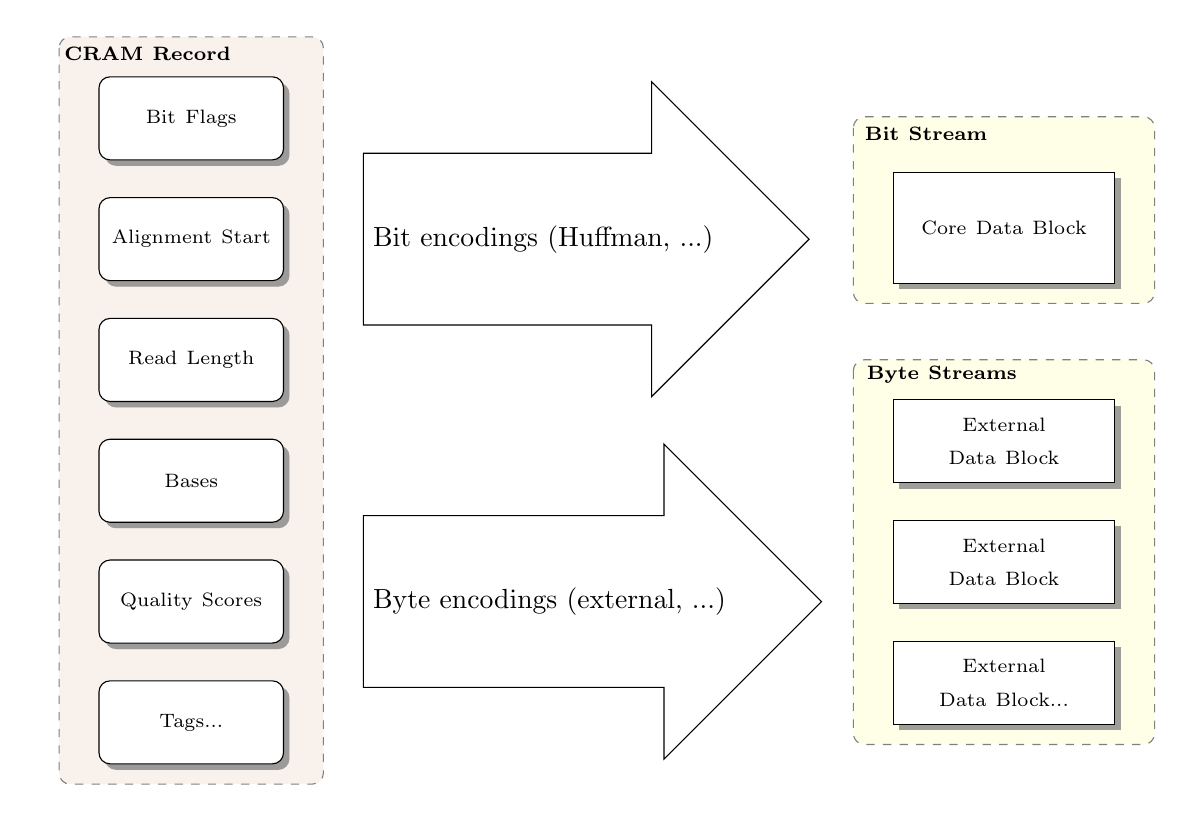
\begin{tikzpicture}

\usetikzlibrary{shapes, shadows, positioning, arrows,  decorations.markings}

\pgfdeclarelayer{background}
\pgfsetlayers{background,main}

\tikzstyle{dsbox} = [blockbox, text width=6em, minimum width=6em, minimum height=3em, rounded corners, drop shadow]
\tikzstyle{blockbox}=[draw, fill=white, text width=4.0em, text centered, minimum height=1.0em, drop shadow]
\tikzstyle{encodedblocklarge} = [blockbox, text width=6em, minimum width=8em, minimum height=4em, drop shadow]
\tikzstyle{encodedblock} = [blockbox, text width=6em, minimum width=8em, minimum height=3em, drop shadow]

\tikzstyle{texto} = [above, text width=8em, text centered]

\newcommand{\cramRecord}[6]{%
\begin{pgfonlayer}{background}
    \path (#1.west |- #1.north) + (-0.5, 0.5) node (a1) {};
    \path (#1.east |- #6.south) + (+0.5,-0.25) node (a2) {};
    \path[fill=brown!10,rounded corners, draw=black!50, dashed]
      (a1) rectangle (a2);
    \path (a1.east |- a1.south) + (1.0,-0.3) node[texto]
      {\scriptsize\textbf{CRAM Record}};
\end{pgfonlayer}}

\newcommand{\dsbox}[2]{node (p#1) [dsbox]
{\scriptsize{#2}}}
\newcommand{\encodedblock}[2]{node (p#1) [encodedblock]
	{\scriptsize{#2}}}
\newcommand{\encodedblocklarge}[2]{node (p#1) [encodedblocklarge]
   {\scriptsize{#2}}}

\path +(-2.5,-1.5) \dsbox{1}{Bit Flags};
\path (p1.south)+(0.0,-1.0) \dsbox{2}{Alignment Start};
\path (p2.south)+(0.0,-1.0) \dsbox{3}{Read Length};
\path (p3.south)+(0.0,-1.0) \dsbox{4}{Bases};
\path (p4.south)+(0.0,-1.0) \dsbox{5}{Quality Scores};
\path (p5.south)+(0.0,-1.0) \dsbox{6}{Tags...};

\cramRecord{p1}{p2}{p3}{p4}{p5}{p6}

\newcommand{\blockStreams}[4]{%
\begin{pgfonlayer}{background}
    \path (#1.west |- #1.north)+(-0.5, .7) node (a1) {};
    \path (#1.east |- #1.south)+(+0.5, -0.25) node (a2) {};
    \path (#2.west |- #2.north)+(-0.5, 0.5) node (a3) {};
    \path (#4.east |- #4.south)+(+0.5, -0.25) node (a4) {};
    \path[fill=yellow!10, rounded corners, draw=black!50, dashed]
      (a1) rectangle (a2);
    \path (a1.east |- a1.south)+(0.8,-0.3) node[texto]
      {\scriptsize\textbf{Bit Stream}};
    \path[fill=yellow!10, rounded corners, draw=black!50, dashed]
      (a3) rectangle (a4);
    \path (a3.east |- a3.south)+(1.0,-0.3) node[texto]{\scriptsize\textbf{Byte Streams}};
\end{pgfonlayer}}

\path (a1.south) + (12.0, -2.3) \encodedblocklarge {7} {Core Data Block};
\path (p7.south) + (0.0, -2.0) \encodedblock {8} {External Data Block};
\path (p8.south) + (0.0, -1.0) \encodedblock {9} {External Data Block}; 
\path (p9.south) + (0.0, -1.0) \encodedblock {10}{External Data Block...};

\blockStreams {p7} {p8} {p9} {p10}

\node[minimum size=4cm, right = of p2, single arrow, draw, single arrow head indent=0ex, black] {Bit encodings (Huffman, ...) };

\node[minimum size=4cm, right = of p5, single arrow, draw, single arrow head indent=0ex, black] {Byte encodings (external, ...) };

\end{tikzpicture}

Figure 5: The relationship between core and external encodings, and core and external data blocks.

\end{center}

The picture shows how a CRAM record (on the left) is distributed between the core 
data block and one or more external data blocks, via core or external encodings. The specific 
encodings presented are only examples for purposes of illustration. The main point is 
to distinguish between core bit encodings whose output is always stored in a core data 
block, and external byte encodings whose output is always stored in external data 
blocks.

\section{\textbf{End of file container}}

A special container is used to mark the end of a file or stream. It is required in version 3 or later. The idea is to provide an easy and a quick way to detect that a CRAM file or stream is complete. The marker is basically an empty container with ref seq id set to -1 (unaligned) and alignment 
start set to 4542278.

Here is a complete content of the EOF container explained in detail:

\begin{tabular}{|l|l|>{\raggedright}p{150pt}|>{\raggedright}p{180pt}|}
\hline
\textbf{hex bytes} & \textbf{data type} & \textbf{decimal value} & \textbf{field 
name}\tabularnewline
\hline
\multicolumn{4}{|l|}{\textit{Container header}}\tabularnewline
\hline
0f 00 00 00 & integer & 15 & size of blocks data\tabularnewline
\hline
ff ff ff ff 0f & itf8 & -1 & ref seq id\tabularnewline
\hline
e0 45 4f 46 & itf8 & 4542278 & alignment start\tabularnewline
\hline
00 & itf8 & 0 & alignment span\tabularnewline
\hline
00 & itf8 & 0 & number of records\tabularnewline
\hline
00 & itf8 & 0 & global record counter\tabularnewline
\hline
00 & itf8 & 0 & bases\tabularnewline
\hline
01 & itf8 & 1 & block count\tabularnewline
\hline
00 & array & 0 & landmarks\tabularnewline
\hline
05 bd d9 4f & integer & 1339669765 & container header CRC32\tabularnewline
\hline
\multicolumn{4}{|l|}{\textit{Compression header block}}\tabularnewline
\hline
00 & byte & 0 (RAW) & compression method\tabularnewline
\hline
01 & byte & 1 (COMPRESSION\_HEADER) & block content type\tabularnewline
\hline
00 & itf8 & 0 & block content id\tabularnewline
\hline
06 & itf8 & 6 & compressed size\tabularnewline
\hline
06 & itf8 & 6 & uncompressed size\tabularnewline
\hline
\multicolumn{4}{|l|}{\textit{Compression header}}\tabularnewline
\hline
01 & itf8 & 1 & preservation map byte size\tabularnewline
\hline
00 & itf8 & 0 & preservation map size\tabularnewline
\hline
01 & itf8 & 1 & encoding map byte size\tabularnewline
\hline
00 & itf8 & 0 & encoding map size\tabularnewline
\hline
01 & itf8 & 1 & tag encoding byte size\tabularnewline
\hline
00 & itf8 & 0 & tag encoding map size\tabularnewline
\hline
ee 63 01 4b & integer & 1258382318 & block CRC32\tabularnewline
\hline
\end{tabular}

When compiled together the EOF marker is 38 bytes long and in hex representation 
is:

0f 00 00 00 ff ff ff ff 0f e0 45 4f 46 00 00 00 00 01 00 05 bd d9 4f 00 01 00 06 06 01 00 01 00 01 00 ee 63 01 4b

\section{\textbf{Record structure}}
\label{sec:record}

CRAM record is based on the SAM record but has additional features allowing for 
more efficient data storage.  In contrast to BAM record CRAM record uses bits as 
well as bytes for data storage. This way, for example, various coding techniques 
which output variable length binary codes can be used directly in CRAM. On the 
other hand, data series that do not require binary coding can be stored separately 
in external blocks with some other compression applied to them independently.

As CRAM data series may be interleaved within the same blocks\footnote{Interleaving can sometimes provide better compression, however it also adds dependency between types of data meaning it is not possible to selectively decode one data series if it co-locates with another data series in the same block.} understanding the order in which CRAM data series must be decoded is vital.

The overall flowchart is below, with more detailed description in the subsequent sections.

\algnewcommand\algorithmicto{\text{ \textbf{to} }}

\subsection{\textbf{CRAM record}}

Both mapped and unmapped reads start with the following fields. Please note that 
the data series type refers to the logical data type and the data series name corresponds 
to the data series encoding map.

\begin{tabular}{|>{\raggedright}p{70pt}|>{\raggedright}p{75pt}|>{\raggedright}p{90pt}|>{\raggedright}p{171pt}|}
\hline
\textbf{Data series type} & \textbf{Data series name} & \textbf{Field} & \textbf{Description}\tabularnewline
\hline
int & BF & BAM bit flags & see BAM bit flags below\tabularnewline
\hline
int & CF & CRAM bit flags & see CRAM bit flags below\tabularnewline
\hline
- & - & Positional data & See section \ref{subsec:positions}\tabularnewline
\hline
- & - & Read names & See section \ref{subsec:names}\tabularnewline
\hline
- & - & Mate records & See section \ref{subsec:mate}\tabularnewline
\hline
- & - & Auxiliary tags & See section \ref{subsec:tags}\tabularnewline
\hline
- & - & Sequences & See sections \ref{subsec:mapped} and \ref{subsec:unmapped}\tabularnewline
\hline
\end{tabular}

\subsubsection*{\textbf{BAM bit flags (BF data series)}}

The following flags are duplicated from the SAM and BAM specification, with identical meaning.
Note however some of these flags can be derived during decode, so may be omitted in the CRAM file and the bits computed based on both reads of a pair-end library residing within the same slice.

\begin{threeparttable}[t]
\begin{tabular}{|>{\raggedright}p{144pt}|>{\raggedright}p{144pt}|>{\raggedright}p{144pt}|}
\hline
\textbf{Bit flag} & \textbf{Comment} & \textbf{Description}\tabularnewline
\hline
0x1 &  & template having multiple segments in sequencing\tabularnewline
\hline
0x2 &  & each segment properly aligned according to the aligner\tabularnewline
\hline
0x4 &  & segment unmapped\tnote{a}\tabularnewline
\hline
0x8 & calculated\tnote{b}\ \ or stored in the mate's info & next segment in template unmapped\tabularnewline
\hline
0x10 &  & SEQ being reverse complemented\tabularnewline
\hline
0x20 & calculated\tnote{b}\ \ or stored in the mate's info & SEQ of the next segment in the
template being reverse complemented\tabularnewline
\hline
0x40 &  & the first segment in the template\tnote{c}\tabularnewline
\hline
0x80 &  & the last segment in the template\tnote{c}\tabularnewline
\hline
0x100 &  & secondary alignment\tabularnewline
\hline
0x200 &  & not passing quality controls\tabularnewline
\hline
0x400 &  & PCT or optical duplicate\tabularnewline
\hline
0x800 &  & Supplementary alignment\tabularnewline
\hline
\end{tabular}
\begin{tablenotes}
\item[a] Bit 0x4 is the only reliable place to tell whether the read is unmapped.  If 0x4 is set, no assumptions may be made about bits 0x2, 0x100 and 0x800.
\item[b] For segments within the same slice.
\item[c] Bits 0x40 and 0x80 reflect the read ordering within each template inherent in the sequencing technology used, which may be independent from the actual mapping orientation.
If 0x40 and 0x80 are both set, the read is part of a linear template (one where the template sequence is expected to be in a linear order), but it is neither the first nor the last read.
If both 0x40 and 0x80 are unset, the index of the read in the template is unknown.
This may happen for a non-linear template (such as one constructed by stitching together other templates) or when this information is lost during data processing.
\end{tablenotes}
\end{threeparttable}

\subsubsection*{\textbf{CRAM bit flags (CF data series)}}

The CRAM bit flags (also known as compression bit flags) expressed as an integer represent the CF data series. 
The following compression flags are defined for each CRAM read record:

\begin{tabular}{|>{\raggedright}p{39pt}|>{\raggedright}p{150pt}|>{\raggedright}p{242pt}|}
\hline
\textbf{Bit flag} & \textbf{Name} & \textbf{Description}\tabularnewline
\hline
0x1 & quality scores stored as array & quality scores can be stored as read features
or as an array similar to read bases.\tabularnewline
\hline
0x2 & detached & mate information is stored verbatim (e.g. because the pair spans multiple slices or the fields differ to the CRAM computed method)\tabularnewline
\hline
0x4 & has mate downstream & tells if the next segment should be expected further
in the stream\tabularnewline
\hline
0x8 & decode sequence as ``*'' & informs the decoder that the sequence
is unknown and that any encoded reference differences are present only to
recreate the CIGAR string.\tabularnewline
\hline
\end{tabular}


The following pseudocode describes the general process of decoding an entire CRAM record.
The sequence data itself is in one of two encoding formats depending on whether the record is aligned (mapped).

\subsubsection*{\textbf{Decode pseudocode}}
\newlength{\maxwidth}
\newcommand{\algalign}[2] % #1 = text to left, #2 = text to right
{\makebox[\maxwidth][l]{$#1{}$}${}#2$}

\begin{algorithmic}[1]
\Procedure{DecodeRecord}{}
\settowidth{\maxwidth}{CRAM\_flags\quad}
\State \algalign{BAM\_flags}{\gets}  \Call{ReadItem}{BF, Integer}
\State \algalign{CRAM\_flags}{\gets} \Call{ReadItem}{CF, Integer}
\State \Call{DecodePositions}{}\Comment{See section \ref{subsec:positions}}
\State \Call{DecodeNames}{}\Comment{See section \ref{subsec:names}}
\State \Call{DecodeMateData}{}\Comment{See section \ref{subsec:mate}}
\State \Call{DecodeTagData}{}\Comment{See section \ref{subsec:tags}}
\Statex

\If{$(BF$ AND $4) \ne 0$}\Comment{Unmapped flag}
  \State \Call{DecodeMappedRead}{}\Comment{See section \ref{subsec:mapped}}
\Else
  \State \Call{DecodeUnmappedRead}{}\Comment{See section \ref{subsec:unmapped}}
\EndIf
\EndProcedure
\end{algorithmic}

\subsection{\textbf{CRAM positional data}}
\label{subsec:positions}

Following the bit-wise BAM and CRAM flags, CRAM encodes positional related data including reference, alignment positions and length, and read-group.
Positional data is stored for both mapped and unmapped sequences, as unmapped data may still be ``placed'' at a specific location in the genome (without being aligned).
Typically this is done to keep a sequence pair (paired-end or mate-pair sequencing libraries) together when one of the pair aligns and the other does not.

For reads stored in a position-sorted slice, the AP-delta flag in the compression header preservation map should be set and the AP data series will be delta encoded, using the slice alignment-start value as the first position to delta against.
Note for multi-reference slices this may mean that the AP series includes negative values, such as when moving from an alignment to the end of one reference sequence to the start of the next or to unmapped unplaced data.  When the AP-delta flag is not set the AP data series is stored as a normal integer value.

\begin{tabular}{|>{\raggedright}p{70pt}|>{\raggedright}p{75pt}|>{\raggedright}p{90pt}|>{\raggedright}p{171pt}|}
\hline
\textbf{Data series type} & \textbf{Data series name} & \textbf{Field} & \textbf{Description}\tabularnewline
\hline
int & RI & ref id & reference sequence id (only present in multiref slices)\tabularnewline
\hline
int & RL & read length & the length of the read\tabularnewline
\hline
int & AP & alignment start & the alignment start position\tabularnewline
\hline
int & RG & read group & the read group identifier expressed as the N\textsuperscript{th} record in the header, starting from 0 with -1 for no group\tabularnewline
\hline
\end{tabular}

\vskip 20pt
\begin{algorithmic}[1]
\Procedure{DecodePositions}{}
\If{$slice\_header.reference\_sequence\_id = -2$}
  \State $reference\_id\gets$ \Call{ReadItem}{RI, Integer}
\Else
  \State $reference\_id\gets slice\_header.reference\_sequence\_id$
\EndIf
\State $read\_length \gets$ \Call{ReadItem}{RL, Integer}
\If{$container\_pmap.AP\_delta \ne 0$}
    \If{$first\_record\_in\_slice$}
        \State $last\_position\gets$ $slice\_header.alignment\_start$
    \EndIf
    \State $alignment\_position \gets$ \Call{ReadItem}{AP, Integer} + $last\_position$
    \State $last\_position \gets alignment\_position$
\Else
    \State $alignment\_position \gets$ \Call{ReadItem}{AP, Integer}
\EndIf
\State $read\_group \gets$ \Call{ReadItem}{RG, Integer}
\EndProcedure
\end{algorithmic}

\subsection{Read names (RN data series)}
\label{subsec:names}

Read names can be preserved in the CRAM format, but this is optional and is governed by the \texttt{RN} preservation map key in the container compression header. See section \ref{subsec:compression-header}.
When read names are not preserved the CRAM decoder should generate names, typically based on the file name and a numeric ID of the read using the record counter field of the slice header block.
Note read names may still be preserved even when the \texttt{RN} compression header key indicates otherwise, such as where a read is part of a read-pair and the pair spans multiple slices.
In this situation the record will be marked as detached (see the CF data series) and the mate data below (section \ref{subsec:mate}) will contain the read name.

\begin{tabular}{|>{\raggedright}p{70pt}|>{\raggedright}p{75pt}|>{\raggedright}p{90pt}|>{\raggedright}p{171pt}|}
\hline
\textbf{Data series type} & \textbf{Data series name} & \textbf{Field} & \textbf{Description}\tabularnewline
\hline
byte[ ] & RN & read names & read names\tabularnewline
\hline
\end{tabular}

\vskip 20pt
\begin{algorithmic}[1]
\Procedure{DecodeNames}{}
\If{$container\_pmap.read\_names\_included = 1$}
  \State $read\_name \gets$ \Call{ReadItem}{RN, Byte[]}
\Else
  \State $read\_name \gets$ \Call{GenerateName}{}
\EndIf
\Statex
\EndProcedure
\end{algorithmic}

\subsection{\textbf{Mate records}}
\label{subsec:mate}

There are two ways in which mate information can be preserved in CRAM.
If the next fragment is not in the same slice we store verbatim copies of the insert size, mate reference chromosome and positions, and mate flags (mapped status, orientation) for both records.
In this case both records are labelled as ``detached'' in the CF data series using bit 2.

If this and the next fragment are within the same slice, we can derive much of this information by comparing the two records.
The upstream record has CF bit 4 (mate downstream) flag set and stores the number of records to skip (in the NF data series) between this record and the record for the next fragment on this template, with zero meaning the next fragment is also the next record.
The downstream record has neither CF bits 2 (detached) or 4 (mate downstream) set nor does it use the NF data series (unless it also has an additional ``next fragment'' to refer to).

It is not mandatory to use this deduplication approach and optionally CRAM write implementations may wish to label data as detached even when all records for the template reside in the same slice.
One reason to do this may be to preserve inconsistent data so that it round-trips through the CRAM format with full fidelity

\begin{tabular}{|>{\raggedright}p{68pt}|>{\raggedright}p{115pt}|>{\raggedright}p{228pt}|}
\hline
\textbf{Data series type} & \textbf{Data series name} & \textbf{Description}\tabularnewline
\hline
int & NF & the number of records to skip to the next fragment\tabularnewline
\hline
\end{tabular}

In the above case, the NS (mate reference name), NP (mate position) and TS (template size) fields for both records should be derived once the mate has also been decoded.
Mate reference name and position are obvious and simply copied from the mate.
The template size is computed using the method described in the SAM specification; the inclusive distance from the leftmost to rightmost mapped bases with the sign being positive for the leftmost record and negative for the rightmost record.

If the next fragment is not found within this slice then the following structure is included into the CRAM record.
Note there are cases where read-pairs within the same slice may be marked as detached and use this structure, such as to store mate-pair information that does not match the algorithm used by CRAM for computing the mate data on-the-fly.

\begin{tabular}{|>{\raggedright}p{66pt}|>{\raggedright}p{117pt}|>{\raggedright}p{228pt}|}
\hline
\textbf{Data series type} & \textbf{Data series name} & \textbf{Description}\tabularnewline
\hline
int & MF & next mate bit flags, see table below\tabularnewline
\hline
byte[ ] & RN & the read name (if and only if not known already)\tabularnewline
\hline
int & NS & mate reference sequence identifier \tabularnewline
\hline
int & NP & mate alignment start position \tabularnewline
\hline
int & TS & the size of the template (insert size)\tabularnewline
\hline
\end{tabular}

\subsubsection*{Next mate bit flags (MF data series)}

The next mate bit flags expressed as an integer represent the MF data series.
These represent the missing bits we excluded from the BF data series (when compared to the full SAM/BAM flags).
The following bit flags are defined:

\begin{tabular}{|>{\raggedright}p{47pt}|>{\raggedright}p{134pt}|>{\raggedright}p{250pt}|}
\hline
\textbf{Bit flag} & \textbf{Name} & \textbf{Description}\tabularnewline
\hline
0x1 & mate negative strand bit & the bit is set if the mate is on the negative
strand\tabularnewline
\hline
0x2 & mate unmapped bit & the bit is set if the mate is unmapped\tabularnewline
\hline
\end{tabular}


\subsubsection*{\textbf{Decode mate pseudocode}}

In the following pseudocode we are assuming the current record is $this$ and its mate is $next\_frag$.

\begin{algorithmic}[1]
\Procedure{DecodeMateData}{}
\If{$CF$ AND $2$}\Comment{Detached from mate}
  \State $mate\_flags\gets $ \Call{ReadItem}{MF,Integer}
  \If{$mate\_flags$ AND 1}
    \State $bam\_flags\gets bam\_flags$\ OR\ 0x20\Comment{Mate is reverse-complemented}
  \EndIf
  \If{$mate\_flags$ AND 2}
    \State $bam\_flags\gets bam\_flags$\ OR\ 0x08\Comment{Mate is unmapped}
  \EndIf
  \If{$container\_pmap.read\_names\_included \ne 1$}
    \State $read\_name \gets$ \Call{ReadItem}{RN, Byte[]}
  \EndIf
\settowidth{\maxwidth}{mate\_position\ }
\State \algalign{mate\_ref\_id}{\gets}  \Call{ReadItem}{NS, Integer}
\State \algalign{mate\_position}{\gets} \Call{ReadItem}{NP, Integer}
\State \algalign{template\_size}{\gets} \Call{ReadItem}{TS, Integer}
\ElsIf{$CF$ AND $4$}\Comment{Mate is downstream}
  \If{$next\_frag.bam\_flags$ AND 0x10}
    \State $this.bam\_flags \gets this.bam\_flags$\ OR\ 0x20\Comment{next segment reverse complemented}
  \EndIf
  \If{$next\_frag.bam\_flags$ AND 0x04}
    \State $this.bam\_flags \gets this.bam\_flags$\ OR\ 0x08\Comment{next segment unmapped}
  \EndIf
  \State $next\_frag\gets$ \Call{ReadItem}{NF,Integer}
  \State $next\_record\gets this\_record + next\_frag + 1$
  \State Resolve $mate\_ref\_id$ for $this\_record$ and $next\_record$ once both have been decoded
  \State Resolve $mate\_position$ for $this\_record$ and $next\_record$ once both have been decoded
  \State Find leftmost and rightmost mapped coordinate in records $this\_record$ and $next\_record$.
  \State For leftmost of $this\_record$ and $next\_record$: $template\_size\gets rightmost-leftmost+1$
  \State For rightmost of $this\_record$ and $next\_record$: $template\_size\gets -(rightmost-leftmost+1)$
\EndIf
\EndProcedure
\end{algorithmic}

Note as with the SAM specification a template may be permitted to have more than two alignment records.
In this case the ``mate'' for each record is considered to be the next record, with the mate for the last record being the first to form a circular list.
The above algorithm is a simplification that does not deal with this scenario.
The full method needs to observe when record $this+NF$ is also labelled as having an additional mate downstream.
One recommended approach is to resolve the mate information in a second pass, once the entire slice has been decoded.
The final segment in the mate chain needs to set $bam\_flags$ fields 0x20 and 0x08 accordingly based on the first segment.
This is also not listed in the above algorithm, for brevity.

\subsection{Auxiliary tags}
\label{subsec:tags}

Tags are encoded using a tag line (TL data series) integer into the tag dictionary (TD field in the compression header preservation map, see section \ref{subsec:compression-header}).
See section \ref{subsubsec:tags} for a more detailed description of this process.

\begin{tabular}{|>{\raggedright}p{70pt}|>{\raggedright}p{75pt}|>{\raggedright}p{90pt}|>{\raggedright}p{200pt}|}
\hline
\textbf{Data series type} & \textbf{Data series name} & \textbf{Field} & \textbf{Description}\tabularnewline
\hline
int & TL & tag line & an index into the tag dictionary (TD)\tabularnewline
\hline
* & ??? & tag name/type & 3 character key (2 tag identifier and 1 tag type), as specified by the tag dictionary\tabularnewline
\hline
\end{tabular}

\vskip 20pt
\begin{algorithmic}[1]
\Procedure{DecodeTagData}{}
\State $tag\_line\gets$ \Call{ReadItem}{TL,Integer}
\ForAll {$ele \in container\_pmap.tag\_dict(tag\_line)$}
  \State $name\gets$ first two characters of $ele$
  \State $tag(type)\gets$ last character of $ele$
  \State $tag(name)\gets$ \Call{ReadItem}{$ele$, Byte[]}
\EndFor
\EndProcedure
\end{algorithmic}

In the above procedure, $name$ is a two letter tag name and $type$ is one of the permitted types documented in the SAM/BAM specification.
Type is \texttt{c} (signed 8-bit integer), \texttt{C} (unsigned 8-bit integer), \texttt{s} (signed 16-bit integer), \texttt{S} (unsigned 16-bit integer), \texttt{i} (signed 32-bit integer), \texttt{I} (unsigned 32-bit integer), \texttt{f} (32-bit float), \texttt{Z} (nul-terminated string), \texttt{H} (nul-terminated string of hex digits) and \texttt{B} (binary data in array format with the first byte being one of c,C,s,S,i,I,f using the meaning above, a 32-bit integer for the number of array elements, followed by array data encoded using the specified format).  All integers are little endian encoded.

For example a SAM tag \texttt{MQ:i} has name \texttt{MQ} and type \texttt{i} and will be decoded using one of MQc, MQC, MQs, MQS, MQi and MQI data series depending on size and sign of the integer value.

Note some auxiliary tags can be created automatically during decode so can optionally be removed by the encoder.
However if the decoder finds a tag stored verbatim it should use this in preference to automatically computing the value.

The RG (read group) auxiliary tag should be created if the read group (RG data series) value is not $-1$.

The MD and NM auxiliary tags store the differences (an edit string) between the sequence and the reference along with the number of mismatches.
These may optionally be created on-the-fly during reference-based sequence reconstruction and should match the description provided in the SAMtags document.
An encoder may decide to store these verbatim when no reference is used or where the automatically constructed values differ to the input data.

Note there is no mechanism to describe which records have MD/NM present and which do not.
If this is deemed important, the only recourse is to store all MD and NM verbatim and to request that the decoding software does not automatically generate its own for records that have no stored MD and NM tags.

\subsection{\textbf{Mapped reads}}
\label{subsec:mapped}

\subsubsection*{\textbf{Read feature records}}
\label{subsec:features}

Read features are used to store read details that are expressed using read coordinates 
(e.g. base differences respective to the reference sequence). The read feature 
records start with the number of read features followed by the read features themselves.
Finally the single mapping quality and per-base quality scores are stored.

\begin{threeparttable}[t]
\begin{tabular}{|>{\raggedright}p{88pt}|>{\raggedright}p{83pt}|>{\raggedright}p{85pt}|>{\raggedright}p{180pt}|}
\hline
\textbf{Data series type} & \textbf{Data series name} & \textbf{Field} & \textbf{Description}\tabularnewline
\hline
int & FN & number of read features & the number of read features\tabularnewline
\hline
int & FP & in-read-position\tnote{a} & position of the read feature\tabularnewline 
\hline
byte & FC & read feature code\tnote{a} & See feature codes below\tabularnewline
\hline
* & * & read feature data\tnote{a} & See feature codes below\tabularnewline
\hline
int & MQ & mapping qualities & mapping quality score\tabularnewline
\hline
byte[read length] & QS & quality scores & the base qualities, if preserved\tabularnewline
\hline
\end{tabular}
\begin{tablenotes}
\item[a] Repeated FN times, once for each read feature.
\end{tablenotes}
\end{threeparttable}

\subsubsection*{Read feature codes}

Each feature code has its own associated data series containing further information specific to that feature.
The following codes are used to distinguish variations in read coordinates:

\begin{tabular}{|>{\raggedright}p{91pt}|>{\raggedright}p{45pt}|>{\raggedright}p{72pt}|>{\raggedright}p{66pt}|>{\raggedright}p{132pt}|}
\hline
\textbf{Feature code} & \textbf{Id} & \textbf{Data series type} & \textbf{Data 
series name} & \textbf{Description}\tabularnewline
\hline
Bases & b (0x62) & byte[ ] & BB & a stretch of bases\tabularnewline
\hline
Scores & q (0x71) & byte[ ] & QQ & a stretch of scores\tabularnewline
\hline
% Neither C nor Java implementations generator nor can decode the 'A'
% feature code, but if they did they'd be BB/QQ and not BA/QS.  Best
% to omit it from published spec for now?
%
% Bases and scores & A (0x41) & byte[ ],byte[ ] & BB,QQ & A a stretch of bases and
% quality scores score\tabularnewline
% \hline
Read base & B (0x42) & byte,byte & BA,QS & A base and associated quality score\tabularnewline
\hline
Substitution & X (0x58) & byte & BS & base substitution codes, SAM operators X, 
M and =\tabularnewline
\hline
Insertion & I (0x49) & byte[ ] & IN & inserted bases, SAM operator I\tabularnewline
\hline
Deletion & D (0x44) & int & DL & number of deleted bases, SAM operator D\tabularnewline
\hline
Insert base & i (0x69) & byte & BA & single inserted base, SAM operator I\tabularnewline
\hline
Quality score & Q (0x51) & byte & QS & single quality score\tabularnewline
\hline
Reference skip & N (0x4E) & int & RS & number of skipped bases, SAM operator N\tabularnewline
\hline
Soft clip & S (0x53) & byte[ ] & SC & soft clipped bases, SAM operator S\tabularnewline
\hline
Padding & P (0x50) & int & PD & number of padded bases, SAM operator P\tabularnewline
\hline
Hard clip & H (0x48) & int & HC & number of hard clipped bases, SAM operator H\tabularnewline
\hline
\end{tabular}

\subsubsection*{Base substitution codes (BS data series)}

A base substitution is defined as a change from one nucleotide base (reference base) to
another (read base), including N as an unknown or missing base. There are 5 possible reference
bases (ACGTN), with 4 possible substitutions for each base, and 20 substitutions in total.
The codes for all possible substitutions are stored in a substitution matrix. To restore a
base, one would use the reference base and the substitution code, resolving the base via lookup
in the substitution matrix.

\subsubsection*{Substitution Matrix Format}

Each of the 4 possible substitutions for a given reference base is assigned a 2-bit integer
code (see below) with a value ranging from 0 to 3 inclusive. The 4 2-bit codes are packed
into a single byte, high 2-bits first, for each base ACGTN (minus the reference base itself).
The entire substitution matrix is written as 5 such bytes, one for each reference base, also
in the order ACGTN.

\subsubsection*{Substitution Code Assignment}

To assign the susbtitution code for a given reference base/read base, the substitutions for
each reference base may optionally be sorted by their frequencies, in descending order, with
same-frequency ties broken using the fixed order ACGTN. Although sorting by substitution
frequency is not required by the CRAM format, assigning substitution codes based on frequency
maximizes compression by ensuring that the most frequent substitutions use the shortest possible
codes.

For example, let us assume the following substitution frequencies for base A: 

AC: 15\%

AG: 25\%

AT: 55\%

AN: 5\%

Then the substitution codes are: 

AC: 2

AG: 1

AT: 0

AN: 3

The first byte of the substitution matrix entry for reference base A is written as a single byte,
with the codes in the order CGTN: 10 01 00 11 = 147 decimal, or 0x93 in this case. This will then
be followed by 4 more bytes representing substitutions for reference bases C, G, T and N.

\subsubsection*{Decode mapped read pseudocode}

\begin{algorithmic}[1]
\Procedure{DecodeMappedRead}{}
  \State $feature\_number\gets$ \Call{ReadItem}{FN, Integer} 
  \For{$i\gets 1 \algorithmicto feature\_number$}
    \State \Call{DecodeFeature}{}
  \EndFor
  \State $mapping\_quality\gets$ \Call{ReadItem}{MQ, Integer} 
  \If{$CF$ AND $1$}\Comment{Quality stored as an array}
    \For{$i\gets 1 \algorithmicto read\_length$}
      \State $quality\_score\gets$ \Call{ReadItem}{QS, Integer} 
    \EndFor
  \EndIf
\EndProcedure
\Statex
\Procedure{DecodeFeature}{}
    \settowidth{\maxwidth}{feature\_position\ }
    \State \algalign{feature\_code}{\gets}       \Call{ReadItem}{FC, Integer} 
    \State \algalign{feature\_position}{\gets}   \Call{ReadItem}{FP, Integer} 
    \settowidth{\maxwidth}{substitution\_code\ }
    \If{$feature\_code = $`B'}
      \State \algalign{base}{\gets}              \Call{ReadItem}{BA, Byte}
      \State \algalign{quality\_score}{\gets}    \Call{ReadItem}{QS, Byte}
    \ElsIf{$feature\_code = $`X'}
      \State \algalign{substitution\_code}{\gets} \Call{ReadItem}{BS, Byte}
    \ElsIf{$feature\_code = $`I'}
      \State \algalign{inserted\_bases}{\gets}   \Call{ReadItem}{IN, Byte[]}
    \ElsIf{$feature\_code = $`S'}
      \State \algalign{softclip\_bases}{\gets}   \Call{ReadItem}{SC, Byte[]}
    \ElsIf{$feature\_code = $`H'}
      \State \algalign{hardclip\_length}{\gets}  \Call{ReadItem}{HC, Integer}
    \ElsIf{$feature\_code = $`P'}
      \State \algalign{pad\_length}{\gets}       \Call{ReadItem}{PD, Integer}
    \ElsIf{$feature\_code = $`D'}
      \State \algalign{deletion\_length}{\gets}  \Call{ReadItem}{DL, Integer}
    \ElsIf{$feature\_code = $`N'}
      \State \algalign{ref\_skip\_length}{\gets} \Call{ReadItem}{RS, Integer}
    \ElsIf{$feature\_code = $`i'}
      \State \algalign{base}{\gets}              \Call{ReadItem}{BA, Byte}
    \ElsIf{$feature\_code = $`b'}
      \State \algalign{bases}{\gets}             \Call{ReadItem}{BB, Byte[]}
    \ElsIf{$feature\_code = $`q'}
      \State \algalign{quality\_scores}{\gets}   \Call{ReadItem}{QQ, Byte[]}
    \ElsIf{$feature\_code = $`Q'}
      \State \algalign{quality\_score}{\gets}    \Call{ReadItem}{QS, Byte}
    \EndIf
\EndProcedure
\end{algorithmic}

\subsection{\textbf{Unmapped reads}}
\label{subsec:unmapped}

The CRAM record structure for unmapped reads has the following additional fields:

\begin{tabular}{|>{\raggedright}p{88pt}|>{\raggedright}p{83pt}|>{\raggedright}p{85pt}|>{\raggedright}p{180pt}|}
\hline
\textbf{Data series type} & \textbf{Data series name} & \textbf{Field} & \textbf{Description}\tabularnewline
\hline
byte[read length] & BA & bases & the read bases\tabularnewline
\hline
byte[read length] & QS & quality scores & the base qualities, if preserved\tabularnewline
\hline
\end{tabular}

\vskip20pt
\begin{algorithmic}[1]
\Procedure{DecodeUnmappedRead}{}
  \For{$i\gets 1 \algorithmicto read\_length$}
    \State $base\gets$ \Call{ReadItem}{BA, Byte}
  \EndFor
  \If{$CF$ AND $1$}\Comment{Quality stored as an array}
    \For{$i\gets 1 \algorithmicto read\_length$}
      \State $quality\_score\gets$ \Call{ReadItem}{QS, Byte}
    \EndFor
  \EndIf
\EndProcedure
\end{algorithmic}

\section{\textbf{Reference sequences}}

CRAM format is natively based upon usage of reference sequences even though in 
some cases they are not required. In contrast to BAM format CRAM format has strict 
rules about reference sequences. 

\begin{enumerate}
\item M5 (sequence MD5 checksum) field of @SQ sequence record in the BAM header is 
required and UR (URI for the sequence fasta optionally gzipped file) field is strongly 
advised. The rule for calculating MD5 is to remove any non-base symbols (like \textbackslash{}n, 
sequence name or length and spaces) and upper case the rest. Here are some examples: 

\texttt{> samtools faidx human\_g1k\_v37.fasta 1 \textbar{} grep -v '\textasciicircum{}>' \textbar{} tr -d '\textbackslash{}n' \textbar{} tr a-z A-Z \textbar{} md5sum -\\
1b22b98cdeb4a9304cb5d48026a85128  -}

\texttt{> samtools faidx human\_g1k\_v37.fasta 1:10-20 \textbar{}grep -v '\textasciicircum{}\texttt{>}' \textbar{}tr -d '\textbackslash{}n' \textbar{}tr a-z A-Z \textbar{}md5sum -\\
0f2a4865e3952676ffad2c3671f14057  -}

Please note that the latter calculates the checksum for 11 bases from position 
10 (inclusive) to 20 (inclusive) and the bases are counted 1-based, so the first 
base position is 1. 

\item All CRAM reader implementations are expected to check for reference MD5 checksums 
and report any missing or mismatching entries. Consequently, all writer implementations 
are expected to ensure that all checksums are injected or checked during compression 
time. 

\item In some cases reads may be mapped beyond the reference sequence. All out of 
range reference bases are all assumed to be `N'. 

\item MD5 checksum bytes in slice header should be ignored for unmapped or multiref 
slices. 
\end{enumerate}

\section{\textbf{Indexing}}

\subsubsection*{General notes}

Indexing is only valid on coordinate (reference ID and then leftmost position) sorted files.

Please note that CRAM indexing is external to the file format itself and may change 
independently of the file format specification in the future. For example, a new 
type of index file may appear.

Individual records are not indexed in CRAM files, slices should be used instead 
as a unit of random access. Another important difference between CRAM and BAM indexing 
is that CRAM container header and compression header block (first block in container) 
must always be read before decoding a slice. Therefore two read operations are 
required for random access in CRAM.

Indexing a CRAM file is deemed to be a lightweight operation because it usually does not require any CRAM records to be read.
Indexing information can be obtained from container headers, namely sequence id, alignment start and span, container start byte offset and slice byte offset inside the container (landmarks).
The exception to this is with multi-reference containers, where the ``RI'' data series must be read.

\subsubsection*{CRAM index}

A CRAM index is a gzipped tab delimited file containing the following columns:

\begin{enumerate}
\item Reference sequence id

\item Alignment start (ignored on read for unmapped slices, set to 0 on write)

\item Alignment span (ignored on read for unmapped slices, set to 0 on write)

\item Absolute byte offset of Container header in the file.

\item Relative byte offset of the Slice header block, from the end of
the container header.  This is the same as the ``landmark'' field
in the container header.

\item Slice size in bytes (including slice header and all blocks).
\end{enumerate}

Each line represents a slice in the CRAM file.
Please note that all slices must be listed in the index file.

Multi-reference slices may need to have multiple lines for the same slice; one for each reference contained within that slice.
In this case the index reference sequence ID will be the actual reference ID (from the ``RI'' data series) and not -2.

Slices containing solely unmapped unplaced data (reference ID -1) still require values for all columns, although the alignment start and span will be ignored.
It is recommended that they are both set to zero.

To illustrate this the absolute and relative offsets used in a three slice container are shown in the diagram below.

\begin{center}
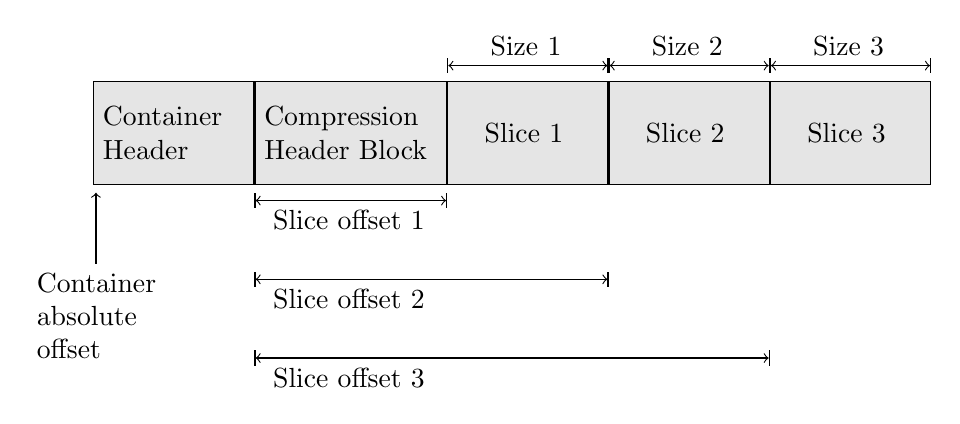
\begin{tikzpicture}[
  boxed/.style={rectangle, draw=black, fill=black!10, minimum height=1.3cm, text width=1.8cm},
]
\node(A) [boxed]{Container Header};
\node(B) [boxed,right,text width=2.2cm] at (A.east){Compression Header Block};
\node(C) [boxed,right] at (B.east){\quad Slice 1};
\node(D) [boxed,right] at (C.east){\quad Slice 2};
\node(E) [boxed,right] at (D.east){\quad Slice 3};

\draw[<-] (A.south west)+(1pt,-0.1cm) -- +(1pt,-1cm)
     node[below, text width=1.5cm]{Container absolute offset};


\draw[|<->|] ([yshift=-0.2cm]B.south west) node[below,xshift=1.2cm]{Slice offset 1}
    -- ([yshift=-0.2cm]B.south east);
\draw[|<->|] ([yshift=-1.2cm]B.south west) node[below,xshift=1.2cm]{Slice offset 2}
    -- ([yshift=-1.2cm]C.south east);
\draw[|<->|] ([yshift=-2.2cm]B.south west) node[below,xshift=1.2cm]{Slice offset 3}
    -- ([yshift=-2.2cm]D.south east);

\draw[|<->|] ([yshift=+0.2cm]C.north west) node[above,xshift=1cm]{Size 1} -- ([yshift=+0.2cm]C.north east);
\draw[|<->|] ([yshift=+0.2cm]D.north west) node[above,xshift=1cm]{Size 2} -- ([yshift=+0.2cm]D.north east);
\draw[|<->|] ([yshift=+0.2cm]E.north west) node[above,xshift=1cm]{Size 3} -- ([yshift=+0.2cm]E.north east);


\end{tikzpicture}
\end{center}

\subsubsection*{BAM index}

BAM indexes are supported by using 4-byte integer pointers called landmarks that 
are stored in container header. BAM index pointer is a 64-bit value with 48 bits 
reserved for the BAM block start position and 16 bits reserved for the in-block 
offset. When used to index CRAM files, the first 48 bits are used to store the 
CRAM container start position and the last 16 bits are used to store the index 
of the landmark in the landmark array stored in  container header. The landmark 
index can be used to access the appropriate slice. 

The above indexing scheme treats CRAM slices as individual records in BAM file. 
This allows to apply BAM indexing to CRAM files, however it introduces some overhead 
in seeking specific alignment start because all preceding records in the slice 
must be read and discarded.

\section{\textbf{Encodings}}
\label{sec:encodings}

% FIXME: we have a mishash of coding, encoding and codec.  We should
% go through the entire document and be consistent.

\subsection{\textbf{Introduction}}

The basic idea for codings is to efficiently represent some values in binary format. 
This can be achieved in a number of ways that most frequently involve some knowledge 
about the nature of the values being encoded, for example, distribution statistics. 
The methods for choosing the best encoding and determining its parameters are very 
diverse and are not part of the CRAM format specification, which only describes 
how the information needed to decode the values should be stored.

Note two of the encodings (Golomb and Golomb-Rice) are listed as deprecated.
These are still formally part of the CRAM specification, but have not been used by the primary implementations and may not be well supported.
Therefore their use is permitted, but not recommended.

\subsubsection*{Offset}

Many of the codings listed below encode positive integer numbers. An integer offset 
value is used to allow any integer numbers and not just positive ones to be encoded. 
It can also be used for monotonically decreasing distributions with the maximum 
not equal to zero. For example, given offset is 10 and the value to be encoded 
is 1, the actually encoded value would be offset+value=11. Then when decoding, 
the offset would be subtracted from the decoded value. 

\subsection{EXTERNAL: codec ID 1}

Can encode types \textit{Byte}, \textit{Integer}.

The EXTERNAL coding is simply storage of data verbatim to an external block with a given ID.
If the type is \textit{Byte} the data is stored as-is, otherwise for \textit{Integer} type the data is stored in ITF8.

\subsubsection*{Parameters}

CRAM format defines the following parameters of EXTERNAL coding: 

\begin{tabular}{|>{\raggedright}p{100pt}|>{\raggedright}p{100pt}|>{\raggedright}p{230pt}|}
\hline
\textbf{Data type} & \textbf{Name} & \textbf{Comment}
\tabularnewline
\hline
itf8 & external id & id of an external block containing the byte stream\tabularnewline
\hline
\end{tabular}

\subsection{Huffman coding: codec ID 3}

Can encode types \textit{Byte}, \textit{Integer}.

Huffman coding replaces symbols (values to encode) by binary codewords, with common symbols having shorter codewords such that the total message of binary codewords is shorter than using uniform binary codeword lengths.
The general process consists of the following steps.

\begin{itemize}
\item Obtain symbol code lengths.
\begin{itemize}
\item If encoding:\\
- Compute symbol frequencies.\\
- Compute code lengths from frequencies.
\item If decoding:\\
- Read code lengths from codec parameters.
\end{itemize}

\item Compute canonical Huffman codewords from code lengths\footnote{\url{https://en.wikipedia.org/wiki/Canonical_Huffman_code}}.

\item Encode or decode bits as per the symbol to codeword table.
Codewords have the ``prefix property'' that no codeword is a prefix of another codeword, enabling unambiguous decode bit by bit.
\end{itemize}

The use of canonical Huffman codes means that we only need to store the code lengths and use the same algorithm in both encoder and decoder to generate the codewords.
This is achieved by ensuring our symbol alphabet has a natural sort order and codewords are assigned in numerical order.

\textbf{Important note: for alphabets with only one value, the codeword will be zero bits long.}
This makes the Huffman codec an efficient mechanism for specifying constant values.

\subsubsection*{Canonical code computation}

\begin{enumerate}
\item Sort the alphabet ascending using bit-lengths and then using numerical order 
of the values.

\item The first symbol in the list gets assigned a codeword which is the same length 
as the symbol's original codeword but all zeros. This will often be a single zero 
('0').

\item Each subsequent symbol is assigned the next binary number in sequence, ensuring
that following codes are always higher in value.

\item When you reach a longer codeword, then after incrementing, append zeros until 
the length of the new codeword is equal to the length of the old codeword.
\end{enumerate}

\subsubsection*{Examples}

\begin{tabular}{|>{\raggedright}p{105pt}|>{\raggedright}p{105pt}|>{\raggedright}p{105pt}|}
\hline
\textbf{Symbol} & \textbf{Code length} & \textbf{Codeword}\tabularnewline
\hline
A & 1 & 0\tabularnewline
\hline
B & 3 & 100\tabularnewline
C & 3 & 101\tabularnewline
D & 3 & 110\tabularnewline
\hline
E & 4 & 1110\tabularnewline
F & 4 & 1111\tabularnewline
\hline
\end{tabular}

\subsubsection*{Parameters}

\begin{tabular}{|>{\raggedright}p{100pt}|>{\raggedright}p{100pt}|>{\raggedright}p{230pt}|}
\hline
\textbf{Data type} & \textbf{Name} & \textbf{Comment}
\tabularnewline
\hline
itf8[ ] & alphabet & list of all encoded symbols (values)\tabularnewline
\hline
itf8[ ] & bit-lengths & array of bit-lengths for each symbol in the alphabet\tabularnewline
\hline
\end{tabular}

\subsection{Byte array coding}

Often there is a need to encode an array of bytes where the length is not predetermined.
For example the read identifiers differ per alignment record, possibly with different lengths, and this length must be stored somewhere.
There are two choices available: storing the length explicitly (BYTE\_ARRAY\_LEN) or continuing to read bytes until a termination value is seen (BYTE\_ARRAY\_STOP).

Note in contrast to this, quality values are known to be the same length as the sequence which is an already known quantity, so this does not need to be encoded using the byte array codecs.

\subsubsection*{BYTE\_ARRAY\_LEN: codec ID 4}

Can encode types \textit{Byte[ ]}.

Byte arrays are captured length-first, meaning that the length of every array element is written using an additional encoding.
For example this could be a HUFFMAN encoding or another EXTERNAL block.
The length is decoded first followed by the data, followed by the next length and data, and so on.

This encoding can therefore be considered as a nested encoding, with each pair of nested encodings containing their own set of parameters.
The byte stream for parameters of the BYTE\_ARRAY\_LEN encoding is therefore the concatenation of the length and value encoding parameters as described in section~\ref{subsec:writing-bytes}.

The parameter for BYTE\_ARRAY\_LEN are listed below:

\begin{tabular}{|>{\raggedright}p{100pt}|>{\raggedright}p{100pt}|>{\raggedright}p{230pt}|}
\hline
\textbf{Data type} & \textbf{Name} & \textbf{Comment}
\tabularnewline
\hline
encoding\texttt{<}int\texttt{>} & lengths encoding & an encoding describing how 
the arrays lengths are captured\tabularnewline
\hline
encoding\texttt{<}byte\texttt{>} & values encoding & an encoding describing how 
the values are captured\tabularnewline
\hline
\end{tabular}

For example, the bytes specifying a BYTE\_ARRAY\_LEN encoding, including the codec and parameters, for a 16-bit X0 auxiliary tag (``X0C'') may use HUFFMAN encoding to specify the length (always 2 bytes) and an EXTERNAL encoding to store the value to an external block with ID 200.

\begin{tabular}{lll}
\hline
\textbf{Bytes} & & \textbf{Meaning}\\
\hline
\texttt{0x04}         & & BYTE\_ARRAY\_LEN codec ID                                    \\
\texttt{0x0a}         & & 10 remaining bytes of BYTE\_ARRAY\_LEN parameters            \\
\\
\texttt{0x03}         & & HUFFMAN codec ID, for aux tag lengths                        \\
\texttt{0x04}         & & 4 more bytes of HUFFMAN parameters                           \\
\texttt{0x01}         & & Alphabet array size = 1                                      \\
\texttt{0x02}         & & alphabet symbol; (length = 2)                                \\
\texttt{0x01}         & & Codeword array size = 1                                      \\
\texttt{0x00}         & & Code length = 0 (zero bits needed as alphabet is size 1)     \\
\\
\texttt{0x01}         & & EXTERNAL codec ID, for aux tag values                        \\
\texttt{0x02}         & & 2 more bytes of EXTERNAL parameters                          \\
\texttt{0x80 0xc8}    & & ITF8 encoding for block ID 200                               \\
\hline
\end{tabular}



\subsubsection*{BYTE\_ARRAY\_STOP: codec ID 5}

Can encode types \textit{Byte[ ]}.

Byte arrays are captured as a sequence of bytes terminated by a special stop byte.
The data returned does not include the stop byte itself.
In contrast to BYTE\_ARRAY\_LEN the value is always encoded with EXTERNAL so the parameter is an external id instead of another encoding.

\begin{tabular}{|>{\raggedright}p{100pt}|>{\raggedright}p{100pt}|>{\raggedright}p{230pt}|}
\hline
\textbf{Data type} & \textbf{Name} & \textbf{Comment}
\tabularnewline
\hline
byte & stop byte & a special byte treated as a delimiter\tabularnewline
\hline
itf8 & external id & id of an external block containing the byte stream\tabularnewline
\hline
\end{tabular}

\subsection{Beta coding: codec ID 6}

Can encode types \textit{Integer}.

\subsubsection*{Definition}

Beta coding is a most common way to represent numbers in \emph{binary notation} and is sometimes referred to as binary coding.
The decoder reads the specified fixed number of bits (most significant first) and subtracts the offset value to get the decoded integer.

\subsubsection*{Parameters}

CRAM format defines the following parameters of beta coding: 

\begin{tabular}{|>{\raggedright}p{144pt}|>{\raggedright}p{144pt}|>{\raggedright}p{144pt}|}
\hline
\textbf{Data type} & \textbf{Name} & \textbf{Comment}\tabularnewline
\hline
itf8 & offset & offset is subtracted from each value during decode\tabularnewline
\hline
itf8 & length & the number of bits used\tabularnewline
\hline
\end{tabular}

\subsubsection*{Examples}

If we have integer values in the range 10 to 15 inclusive, the largest value would traditionally need 4 bits, but with an offset of -10 we can hold values 0 to 5, using a fixed size of 3 bits.
Using fixed Offset and Length coming from the beta parameters, we decode these values as:

\begin{tabular}{|>{\raggedright}p{105pt}|>{\raggedright}p{105pt}|>{\raggedright}p{105pt}|>{\raggedright}p{105pt}|}
\hline
Offset & Length & \textbf{Bits} & \textbf{Value}\tabularnewline
\hline
-10 & 3 & 000 & 10\tabularnewline
\hline
-10 & 3 & 001 & 11\tabularnewline
\hline
-10 & 3 & 010 & 12\tabularnewline
\hline
-10 & 3 & 011 & 13\tabularnewline
\hline
-10 & 3 & 100 & 14\tabularnewline
\hline
-10 & 3 & 101 & 15\tabularnewline
\hline
\end{tabular}

\subsection{Subexponential coding: codec ID 7}

Can encode types \textit{Integer}.

\subsubsection*{Definition}

Subexponential coding\footnote{Fast progressive lossless image compression, Paul G. Howard and Jeffrey Scott Vitter, 1994. \url{http://www.ittc.ku.edu/~jsv/Papers/HoV94.progressive_FELICS.pdf}} is parametrized by a non-negative integer $k$.
For values $n < 2^{k+1}$ subexponential coding produces codewords identical to Rice coding \footnote{\url{https://en.wikipedia.org/wiki/Golomb_coding\#Rice_coding}}.  For larger values it grows logarithmically with $n$.

\subsubsection*{Encoding}

\begin{enumerate}
\item Add $\mathit{offset}$ to $n$.

\item Determine $u$ and $b$ values from $n$
\begin{align*}
b =
\begin{cases}
  \ k                        & \text{ if $n < 2^k$} \\
  \ \lfloor log_{2}n \rfloor & \text{ if $n \ge 2^k$}
\end{cases}
&\
&u =
\begin{cases}
  \ 0     & \text{ if $n < 2^k$} \\
  \ b-k+1 & \text{ if $n \ge 2^k$}
\end{cases}
\end{align*}

\item Write $u$ in unary form; $u$ 1 bits followed by a single 0 bit.

\item Write the bottom $b$-bits of $n$ in binary form.
\end{enumerate}

\subsubsection*{Decoding}

\begin{enumerate}
\item Read $u$ in unary form, counting the number of leading 1s (prefix) in the codeword (discard the trailing 0 bit).

\item Determine $n$ via:
\begin{enumerate}
\item if $u = 0$ then read $n$ as a $k$-bit binary number.
\item if $u \ge 1$ then read $x$ as a $(u + k - 1)$-bit binary. Let $n = 2^{u+k-1} + x$.
\end{enumerate}

\item Subtract $\mathit{offset}$ from $n$.
\end{enumerate}

\subsubsection*{Examples}

\begin{tabular}{|>{\raggedright}p{105pt}|>{\raggedright}p{105pt}|>{\raggedright}p{105pt}|>{\raggedright}p{105pt}|}
\hline
\textbf{Number} & \textbf{Codeword, k=0} & \textbf{Codeword, k=1} & \textbf{Codeword, 
k=2}\tabularnewline
\hline
0 & 0 & 00 & 000\tabularnewline
\hline
1 & 10 & 01 & 001\tabularnewline
\hline
2 & 1100 & 100 & 010\tabularnewline
\hline
3 & 1101 & 101 & 011\tabularnewline
\hline
4 & 111000 & 11000 & 1000\tabularnewline
\hline
5 & 111001 & 11001 & 1001\tabularnewline
\hline
6 & 111010 & 11010 & 1010\tabularnewline
\hline
7 & 111011 & 11011 & 1011\tabularnewline
\hline
8 & 11110000 & 1110000 & 110000\tabularnewline
\hline
9 & 11110001 & 1110001 & 110001\tabularnewline
\hline
10 & 11110010 & 1110010 & 110010\tabularnewline
\hline
\end{tabular}

\subsubsection*{Parameters}

\begin{tabular}{|>{\raggedright}p{100pt}|>{\raggedright}p{100pt}|>{\raggedright}p{230pt}|}
\hline
\textbf{Data type} & \textbf{Name} & \textbf{Comment}
\tabularnewline
\hline
itf8 & offset & offset is subtracted from each value during decode\tabularnewline
\hline
itf8 & k & the order of the subexponential coding\tabularnewline
\hline
\end{tabular}

\subsection{Gamma coding: codec ID 9}

Can encode types \textit{Integer}.

\subsubsection*{Definition}

\emph{Elias gamma code} is a prefix encoding of positive integers. This is a combination 
of unary coding and beta coding. The first is used to capture the number of bits 
required for beta coding to capture the value. 

\subsubsection*{Encoding}

\begin{enumerate}
\item Write it in binary.

\item Subtract $1$ from the number of bits written in step 1 and prepend that many zeros.

\item An equivalent way to express the same process:

\item Separate the integer into the highest power of $2$ it contains ($2N$) and the remaining 
$N$ binary digits of the integer.

\item Encode $N$ in unary; that is, as $N$ zeroes followed by a one.

\item Append the remaining $N$ binary digits to this representation of $N$.
\end{enumerate}

\subsubsection*{Decoding}

\begin{enumerate}
\item Read and count 0s from the stream until you reach the first 1. Call this count 
of zeroes $N$.

\item Considering the one that was reached to be the first digit of the integer, with 
a value of $2N$, read the remaining $N$ digits of the integer.
\end{enumerate}

\subsubsection*{Examples}

\begin{tabular}{|>{\raggedright}p{76pt}|>{\raggedright}p{107pt}|}
\hline
\textbf{Value} & \textbf{Codeword}\tabularnewline
\hline
1 & 1\tabularnewline
\hline
2 & 010\tabularnewline
\hline
3 & 011\tabularnewline
\hline
4 & 00100\tabularnewline
\hline
\end{tabular}

\subsubsection*{Parameters}

\begin{tabular}{|>{\raggedright}p{144pt}|>{\raggedright}p{144pt}|>{\raggedright}p{144pt}|}
\hline
\textbf{Data type} & \textbf{Name} & \textbf{Comment}\tabularnewline
\hline
itf8 & offset & offset to subtract from each value after decode\tabularnewline
\hline
\end{tabular}

\subsection{DEPRECATED: Golomb coding: codec ID 2}

Can encode types \textit{Integer}.

Note this codec has not been used in any known CRAM implementation since before CRAM v1.0.
Nor is it implemented in some of the major software.
Therefore its use is not recommended.

\subsubsection*{Definition}

\emph{Golomb encoding} is a prefix encoding optimal for representation of random 
positive numbers following geometric distribution. 

\subsubsection*{Encoding}

\begin{enumerate}
\item Fix the parameter $M$ to an integer value.

\item For $N$, the number to be encoded, find

\begin{enumerate}
\item quotient $q = \lfloor N/M \rfloor$

\item remainder $r = N \bmod M$
\end{enumerate}

\item Generate Codeword

\begin{enumerate}
\item The Code format : \texttt{<}Quotient Code\texttt{>}\texttt{<}Remainder Code\texttt{>}, 
where

\item Quotient Code (in unary coding)

\begin{enumerate}
\item Write a $q$-length string of 1 bits

\item Write a 0 bit
\end{enumerate}

\item Remainder Code (in truncated binary encoding)

Set $b=\lceil log_{2}(M) \rceil$

\begin{enumerate}
\item If $r < 2^{b}-M$ code $r$ as plain binary using $b-1$ bits.

\item If $r \ge 2^{b}-M$ code the number $r+2^{b}-M$ in plain binary representation 
using $b$ bits.
\end{enumerate}
\end{enumerate}
\end{enumerate}

\subsubsection*{Decoding}

\begin{enumerate}
\item Read $q$ via unary coding: count the number of 1 bits and consume the following 0 bits.
\item Set $b=\lceil log_{2}(M) \rceil$
\item Read $r$ via $b-1$ bits of binary coding
\item If $r \ge 2^{b}-M$
\begin{enumerate}
\item Read 1 single bit, $x$.
\item Set $r = r*2 + x - (2^{b}-M)$
\end{enumerate}
\item Value is $q*M + r - \mathit{offset}$
\end{enumerate}

\subsubsection*{Examples}

\begin{tabular}{|>{\raggedright}p{76pt}|>{\raggedright}p{107pt}|}
\hline
\textbf{Number} & \textbf{Codeword, M=10, (thus b=4)}\tabularnewline
\hline
0 & 0000\tabularnewline
\hline
4 & 0100\tabularnewline
\hline
10 & 10000\tabularnewline
\hline
26 & 1101100\tabularnewline
\hline
42 & 11110010\tabularnewline
\hline
\end{tabular}

\subsubsection*{Parameters}

Golomb coding takes the following parameters: 

\begin{tabular}{|>{\raggedright}p{144pt}|>{\raggedright}p{144pt}|>{\raggedright}p{144pt}|}
\hline
\textbf{Data type} & \textbf{Name} & \textbf{Comment}\tabularnewline
\hline
itf8 & offset & offset is added to each value\tabularnewline
\hline
itf8 & M & the golomb parameter (number of bins)\tabularnewline
\hline
\end{tabular}

\subsection{DEPRECATED: Golomb-Rice coding: codec ID 8}

Can encode types \textit{Integer}.

Note this codec has not been used in any known CRAM implementation since before CRAM v1.0.
Nor is it implemented in some of the major software.
Therefore its use is not recommended.

Golomb-Rice coding is a special case of Golomb coding when the M parameter is a power of 2.
The reason for this coding is that the division operations in Golomb coding can be replaced with bit shift operators as well as avoiding the extra $r < 2^{b}-M$ check.

\section{\textbf{External compression methods}}

External encoding operates on bytes only. Therefore any data series must be translated into bytes before sending data into an external block.
The following methods are defined.
Exact definitions of these methods are in their respective internet links or the ancillary \textit{CRAMcodecs} document found along side this specification.

Integer values are written as ITF8, which then can be translated into an array 
of bytes. 

Strings, like read name, are translated into bytes according to UTF8 rules. In 
most cases these should coincide with ASCII, making the translation trivial.

Each method has an associated numeric code which is defined in Section~\ref{sec:block-struct}.

\subsection{\textbf{Gzip}}

The Gzip specification is defined in RFC 1952.
Gzip in turn is an encapsulation on the Deflate algorithm defined in RFC 1951.

\subsection{\textbf{Bzip2}}

First available in CRAM v2.0.

Bzip2 is a compression method utilising the Burrows Wheeler Transform, Move To Front transform, Run Length Encoding and a Huffman entropy encoder. 
It is often superior to Gzip for textual data.

An informal format specification exists:\\
\url{https://github.com/dsnet/compress/blob/master/doc/bzip2-format.pdf}

\subsection{\textbf{LZMA}}

First available in CRAM v3.0.

LZMA is the Lempel-Ziv Markov chain algorithm.
CRAM uses the xz Stream format to encapsulate this algorithm, as defined in \url{https://tukaani.org/xz/xz-file-format.txt}.

\subsection{\textbf{rANS4x8 codec}}

First available in CRAM v3.0.

rANS is the range-coder variant of the Asymmetric Numerical
System\footnote{J. Duda, \textit{Asymmetric numeral systems: entropy
    coding combining speed of Huffman coding with compression rate of
    arithmetic coding}, \url{http://arxiv.org/abs/1311.2540}}.

``4x8'' refers to 4-way interleaving with 8-bit renormalisation.\newline
This variant of rANS first appeared in CRAM v3.0.

Details of this algorithm have been moved to the \textit{CRAMcodecs} document.

\subsection{\textbf{rANS4x16 codec}}

First available in CRAM v3.1.

``4x16'' refers to 4-way interleaving with 16-bit renormalisation.\newline
This variant of rANS first appeared in CRAM v3.1.

Details of this algorithm are listed in the \textit{CRAMcodecs} document.

\subsection{\textbf{adaptive arithemtic coding}}

First available in CRAM v3.1.

An entropy encoder that is slower but slightly more concise than
rANS.  It achieves this by adapting the probabilities as it compresses
and decompresses instead of using a fixed table.

Details of this algorithm are listed in the \textit{CRAMcodecs} document.

\subsection{\textbf{fqzcomp codec}}

First available in CRAM v3.1.

This is a method dedicated to compression of quality values.

Details of this algorithm are listed in the \textit{CRAMcodecs} document.

\subsection{\textbf{name tokeniser}}

First available in CRAM v3.1.

This is a method dedicated to compression of read names.

Details of this algorithm are listed in the \textit{CRAMcodecs} document.

\section{\textbf{Appendix}}
\subsection{\textbf{Choosing the container size}}

CRAM format does not constrain the size of the containers. However, the following 
should be considered when deciding the container size:

$\bullet$ Data can be compressed better by using larger containers

$\bullet$ Random access performance is better for smaller containers 

$\bullet$ Streaming is more convenient for small containers

$\bullet$ Applications typically buffer containers into memory

We recommend 1 megabyte containers. They are small enough to provide good random access
and streaming performance while being large enough to provide good compression. 
1\MB\ containers are also small enough to fit into the L2 cache of most modern CPUs.

Some simplified examples are provided below to fit data into 1\MB\ containers.

\textbf{Unmapped short reads with bases, read names, recalibrated and original 
quality scores}

We have 10,000 unmapped short reads (100bp) with read names, recalibrated and original 
quality scores. We estimate 0.4 bits/base (read names) + 0.4 bits/base (bases) 
+ 3 bits/base (recalibrated quality scores) + 3 bits/base (original quality scores) 
$\approx$ 7 bits/base. Space estimate is $10\,000 \times 100 \times 7 \bits
\approx 0.9 \MB$. Data could be stored in a single container.

\textbf{Unmapped long reads with bases, read names and quality scores}

We have 10,000 unmapped long reads (10kb) with read names and quality scores. We 
estimate: 0.4 bits/base (bases) + 3 bits/base (original quality scores) $\approx$
3.5 bits/base. Space estimate is $10\,000 \times 10\,000 \times 3.5 \bits
\approx 42 \MB$. Data could be stored in $42 \times 1\MB$ containers.

\textbf{Mapped short reads with bases, pairing and mapping information}

We have 250,000 mapped short reads (100bp) with bases, pairing and mapping information. 
We estimate the compression to be 0.2 bits/base. Space estimate is $250\,000 \times 100
\times 0.2 \bits \approx 0.6 \MB$. Data could be stored in a single
container.

\textbf{Embedded reference sequences}

We have a reference sequence (10Mb). We estimate the compression to be 2 bits/base. 
Space estimate is $10\,000\,000 \times 2 \bits \approx 2.4 \MB$. Data
could be written into three containers: $1\MB + 1\MB + 0.4\MB$.

\newpage

\subsection{CRAM History}

\subsubsection*{Pre-CRAM: 2010}

The primary concepts and ideas of CRAM stem from work at the European
Bioinformatics Institute in 2010 and 2011, published in:

\begin{quote}\small
Markus Hsi-Yang Fritz,
Rasko Leinonen, Guy Cochrane, and Ewan Birney,
\textbf{Efficient storage of high throughput DNA sequencing data using reference-based compression},
{\sl Genome Res.}~2011~21: 734--740;
\href{http://dx.doi.org/doi:10.1101/gr.114819.110}{doi:10.1101/gr.114819.110};
{\sc pmid:}21245279.
\end{quote}

\subsubsection*{CRAM 0.x: 2011}

Vadim Zalunin implemented the ideas in the paper, now named CRAM, in
the Java CRAMtools package.  This included versions from 0.3 to 0.86\footnote{\url{https://github.com/vadimzalunin/crammer/releases}}.

\subsubsection*{CRAM 1.0: 2012}

The first official launch of the CRAM specification, in the Java
CRAMtools package\footnote{\url{https://github.com/enasequence/cramtools}}

This was publicised at \url{https://github.com/enasequence/cramtools}.

\subsubsection*{CRAM 2.0: 2013}

Reimplementing CRAM in C
\footnote{Staden IO\_Lib 1.13.0 and later HTSlib 0.2.0} exposed a number of issues with the
1.0 specification and disparities between the specification text and
the Java implementation.  CRAM 2.0 unified implementation with
specification.

Other changes included:

\begin{itemize}
\item Support for multiple references per container, to permit storage
of highly fragmented assemblies.

\item Soft-clips and inserted bases moved to their own separate
data-series instead of sharing one.

\item Slice headers contain meta-data tracking the number of records
and bases.

\item Corrected the BF (bam flag) data series to match the BAM
specification.

\item Improved encoding of auxiliary tags.
\end{itemize}

\subsubsection*{CRAM 2.1: 2014}

This is the first version to appear in HTSJDK (version 1.127), ported
from the Java CRAMtools package.

\begin{itemize}
\item EOF blocks are added in order to spot truncated files.
\end{itemize}

\subsubsection*{CRAM 3.0: 2014}

Primarily this is an optimisation of size and speed.

\begin{itemize}
\item Inclusion of LZMA compression library.
\item Inclusion of the custom rANS Order-0 and Order-1 entropy encoders.
\item Checksums added to all file format structures to ensure data integrity.
\end{itemize}

\subsubsection*{CRAM 3.1: 2023}

Note: the formal draft appeared in 2019, and was initially
demonstrated in 2016.

This adds new EXTERNAL compression methods, described in the separate
CRAMcodecs document, and expands the list of permitted ``methods'' in
the CRAM Block structure.

The aim of the new compression methods is improved compression, both
performance with the newer SIMD rANS implementation and file size with
custom name tokeniser and quality codec.

The format is otherwise identical to 3.0.

\newpage

\subsection{\textbf{Contributors and Acknowledgements}}

\begin{itemize}
\item
Markus Fritz, Rasko Leinonen, Guy Cochrane and Ewan Birney (EBI):
Initial ideas behind CRAM.

\item Vadim Zalunin (EBI):
Initial JAVA implementation of CRAM and previous maintainer of CRAM specification.

\item James Bonfield (Sanger Institute):
Initial C implementation of CRAM and current maintainer of CRAM
specification.

\item Joel Thibault (Broad Institute):
previous maintainer of CRAM specification.

\item Chris Norman (Broad Institute):
previous maintainer of CRAM specification and worked on
the HTSJDK implementation.

\item Robert Buels (UC Berkeley): First JavaScript implementation of CRAM

\item Michael Macias (St Jude Children's Research Hospital): First Rust implementation of CRAM

\item Other specification contributors include: John Marshall, Rishi Nag,
Kenta Sato, Artem Tarasov and Jason Travis.

\item Plus a big thank you to everyone who has raised GitHub issues
and/or helped us improve the specification in other ways.
\end{itemize}

\end{document}

\title{CRAM format specification (version 3.1)}
\author{samtools-devel@lists.sourceforge.net}
\date{\headdate}
\maketitle


\begin{quote}\small
The master version of this document can be found at
\url{https://github.com/samtools/hts-specs}.\\
This printing is version~\commitdesc\ from that repository,
last modified on the date shown above.
\end{quote}

\begin{center}
\textit{license: Apache 2.0}
\end{center}
\vspace*{1em}

\section{\textbf{Overview}}

This specification describes the CRAM 3.0 and 3.1 formats.

CRAM has the following major objectives:

\begin{enumerate}
\item Significantly better lossless compression than BAM

\item Full compatibility with BAM

\item Effortless transition to CRAM from using BAM files

\item Support for controlled loss of BAM data
\end{enumerate}

The first three objectives allow users to take immediate advantage of the CRAM 
format while offering a smooth transition path from using BAM files. The fourth 
objective supports the exploration of different lossy compression strategies and 
provides a framework in which to effect these choices. Please note that the CRAM 
format does not impose any rules about what data should or should not be preserved. 
Instead, CRAM supports a wide range of lossless and lossy data preservation strategies 
enabling users to choose which data should be preserved.

Data in CRAM is stored either as CRAM records or using one of the general purpose 
compressors (gzip, bzip2). CRAM records are compressed using a number of different 
encoding strategies. For example, bases are reference compressed by encoding base
differences rather than storing the bases themselves.\footnote{Markus Hsi-Yang Fritz,
Rasko Leinonen, Guy Cochrane, and Ewan Birney,
\textbf{Efficient storage of high throughput DNA sequencing data using reference-based compression},
{\sl Genome Res.}~2011~21: 734--740;
\href{http://dx.doi.org/doi:10.1101/gr.114819.110}{doi:10.1101/gr.114819.110};
{\sc pmid:}21245279.}

\section{\textbf{Data types}}

CRAM specification uses logical data types and storage data types; logical data 
types are written as words (e.g. int) while physical data types are written using 
single letters (e.g. i). The difference between the two is that storage data types 
define how logical data types are stored in CRAM. Data in CRAM is stored either 
as bits or bytes. Writing values as bits and bytes is described in detail 
below.

\subsection{\textbf{Logical data types}}

\begin{description}
\item[Byte]\ \newline
Signed byte (8 bits).

\item[Integer]\ \newline
Signed 32-bit integer. 

\item[Long]\ \newline
Signed 64-bit integer. 

\item[Array]\ \newline
An array of any logical data type: array\texttt{<}type\texttt{>}
\end{description}

% \begin{tabular}{ll}
% \textbf{Byte}    & Signed byte (8 bits).  \\
% \\
% \textbf{Integer} & Signed 32-bit integer. \\
% \\
% \textbf{Long}    & Signed 64-bit integer. \\
% \\
% \textbf{Array}   & An array of any logical data type: \texttt{<}type\texttt{>}[ ] \\
% \end{tabular}

\subsection{\textbf{Writing bits to a bit stream}}

A bit stream consists of a sequence of 1s and 0s. The bits are written most significant 
bit first where new bits are stacked to the right and full bytes on the left are 
written out. In a bit stream the last byte will be incomplete if less than 8 bits 
have been written to it. In this case the bits in the last byte are shifted to 
the left.

\subsubsection*{Example of writing to bit stream}

Let's consider the following example. The table below shows a sequence of write 
operations: 

\begin{tabular}{|l|l|l|l|l|}
\hline
\textbf{Operation order} & \textbf{Buffer state before} & \textbf{Written bits} & \textbf{Buffer state after} & \textbf{Issued bytes}\tabularnewline
\hline
1 & 0x0 & 1 & 0x1 & -\tabularnewline
\hline
2 & 0x1 & 0 & 0x2 & -\tabularnewline
\hline
3 & 0x2 & 11 & 0xB & -\tabularnewline
\hline
4 & 0xB & 0000 0111 & 0x7 & 0xB0\tabularnewline
\hline
\end{tabular}

After flushing the above bit stream the following bytes are written: 0xB0 0x70. 
Please note that the last byte was 0x7 before shifting to the left and became 0x70 
after that:

\texttt{> echo "obase=16; ibase=2; 00000111" \textbar{} bc\\
7\\
\\
> echo "obase=16; ibase=2; 01110000" \textbar{} bc\\
70}

And the whole bit sequence: 

\texttt{> echo "obase=2; ibase=16; B070" \textbar{} bc\\
1011000001110000}

When reading the bits from the bit sequence it must be known that only 12 bits 
are meaningful and the bit stream should not be read after that. 

\subsubsection*{Note on writing to bit stream}

When writing to a bit stream both the value and the number of bits in the value 
must be known. This is because programming languages normally operate with bytes 
(8 bits) and to specify which bits are to be written requires a bit-holder, for 
example an integer, and the number of bits in it. Equally, when reading a value 
from a bit stream the number of bits must be known in advance. In case of prefix 
codes (e.g. Huffman) all possible bit combinations are either known in advance 
or it is possible to calculate how many bits will follow based on the first few 
bits. Alternatively, two codes can be combined, where the first contains the number 
of bits to read. 

\subsection{\textbf{Writing bytes to a byte stream}}
\label{subsec:writing-bytes}

The interpretation of byte stream is straightforward. CRAM uses \emph{little endianness}
for bytes when applicable and defines the following storage data types:

\begin{description}

\item[Boolean (bool)]\ \newline
Boolean is written as 1-byte with 0x0 being `false' and 0x1 being `true'.

\item[Integer (int32)]\ \newline
Signed 32-bit integer, written as 4 bytes in little-endian byte order.

\item[Long (int64)]\ \newline
Signed 64-bit integer, written as 8 bytes in little-endian byte order.

\item[ITF-8 integer (itf8)]\ \newline
This is an alternative way to write an integer value. The idea is similar to UTF-8 
encoding and therefore this encoding is called ITF-8 (Integer Transformation Format 
- 8 bit). 

The most significant bits of the first byte have special meaning and are called 
`prefix'. These are 0 to 4 true bits followed by a 0. The number of 1's denote 
the number of bytes to follow. To accommodate 32 bits such representation requires 
5 bytes with only 4 lower bits used in the last byte 5.

\item[LTF-8 long (ltf8)]\ \newline
See ITF-8 for more details. The only difference between ITF-8 and LTF-8 is the 
number of bytes used to encode a single value. To do so 64 bits are required and 
this can be done with 9 byte at most with the first byte consisting of just 1s 
or 0xFF value. 

\item[{Array (array\texttt{<}type\texttt{>})}]\ \newline
A variable sized array with an explicitly written dimension.
Array length is written first as integer (itf8), followed by the elements of the array.

Implicit or fixed-size arrays are also used, written as \textit{type}\texttt{[ ]} or \textit{type}\texttt{[4]} (for example).
These have no explicit dimension included in the file format and instead rely on the specification itself to document the array size.


\item[{Encoding}]\ \newline
Encoding is a data type that specifies how data series have been compressed. Encodings 
are defined as encoding\texttt{<}type\texttt{>} where the type is a logical data 
type as opposed to a storage data type.

An encoding is written as follows. The first integer (itf8) denotes the codec id 
and the second integer (itf8) the number of bytes in the following encoding-specific 
values. 

Subexponential encoding example: 

\begin{tabular}{|l|l|l|}
\hline
\textbf{Value} & \textbf{Type} & \textbf{Name}\tabularnewline
\hline
0x7 & itf8 & codec id\tabularnewline
\hline
0x2 & itf8 & number of bytes to follow\tabularnewline
\hline
0x0 & itf8 & offset\tabularnewline
\hline
0x1 & itf8 & K parameter\tabularnewline
\hline
\end{tabular}

The first byte ``0x7'' is the codec id. 

The next byte ``0x2'' denotes the length of the bytes to follow (2). 

The subexponential encoding has 2 parameters: integer (itf8) offset and integer (itf8) K.

offset = 0x0 = 0

K = 0x1 = 1


\item[{Map}]\ \newline
A map is a collection of keys and associated values. A map with N keys is written 
as follows: 

\begin{tabular}{|l|l|l|l|l|l|l|l|}
\hline
size in bytes & N & key 1 & value 1 & key ... & value ... & key N & value N\tabularnewline
\hline
\end{tabular}

Both the size in bytes and the number of keys are written as integer (itf8). Keys 
and values are written according to their data types and are specific to each map.

\item[String]\ \newline
A string is represented as byte arrays using UTF-8 format. Read names, reference 
sequence names and tag values with type `Z' are stored as UTF-8.

\end{description}


\section{\textbf{Encodings }}

Encoding is a data structure that captures information about compression details 
of a data series that are required to uncompress it. This could be a set of constants 
required to initialize a specific decompression algorithm or statistical properties 
of a data series or, in case of data series being stored in an external block, 
the block content id. 

Encoding notation is defined as the keyword `encoding' followed by its data type 
in angular brackets, for example `encoding\texttt{<}byte\texttt{>}' stands for 
an encoding that operates on a data series of data type `byte'. 

Encodings may have parameters of different data types, for example the EXTERNAL 
encoding has only one parameter, integer id of the external block. The following 
encodings are defined: 

\begin{tabular}{|l|l|>{\raggedright}p{155pt}|>{\raggedright}p{160pt}|}
\hline
\textbf{Codec} & \textbf{ID} & \textbf{Parameters} & \textbf{Comment}\tabularnewline
\hline
NULL & 0 & none & series not preserved\tabularnewline
\hline
EXTERNAL & 1 & int block content id & the block content identifier used to associate 
external data blocks with data series\tabularnewline
\hline
Deprecated (GOLOMB) & 2 & int offset, int M & Golomb coding\tabularnewline
\hline
HUFFMAN & 3 & array\texttt{<}int\texttt{>}, array\texttt{<}int\texttt{>} & coding with int/byte values\tabularnewline
\hline
BYTE\_ARRAY\_LEN & 4 & encoding\texttt{<}int\texttt{>} array length, encoding\texttt{<}byte\texttt{>} 
bytes & coding of byte arrays with array length\tabularnewline
\hline
BYTE\_ARRAY\_STOP & 5 & byte stop, int external block\linebreak{}
content id & coding of byte arrays with a stop value \tabularnewline
\hline
BETA & 6 & int offset, int number of bits & binary coding\tabularnewline
\hline
SUBEXP & 7 & int offset, int K & subexponential coding\tabularnewline
\hline
Deprecated (GOLOMB\_RICE) & 8 & int offset, int log$_{\text{2}}$m & Golomb-Rice coding\tabularnewline
\hline
GAMMA & 9 & int offset & Elias gamma coding\tabularnewline
\hline
\end{tabular}

See section~\ref{sec:encodings} for more detailed descriptions of all the above coding algorithms and their parameters.

\section{\textbf{Checksums}}
The checksumming is used to ensure data integrity. The following checksumming algorithms are used in CRAM.
\subsection{\textbf{CRC32}}
This is a cyclic redundancy checksum 32-bit long with the polynomial 0x04C11DB7. Please refer to \href{http://www.itu.int/rec/recommendation.asp?type=folders&lang=e&parent=T-REC-V.42}{ITU-T V.42} for more details. The value of the CRC32 hash function is written as an integer.
\subsection{\textbf{CRC32 sum}}
CRC32 sum is a combination of CRC32 values by summing up all individual CRC32 values modulo 2\textsuperscript{32}. 

\section{\textbf{File structure}}

The overall CRAM file structure is described in this section. Please refer to other 
sections of this document for more detailed information. 

A CRAM file consists of a fixed length file definition, followed by a CRAM header container,
then zero or more data containers, and finally a special end-of-file container.

\begin{center}
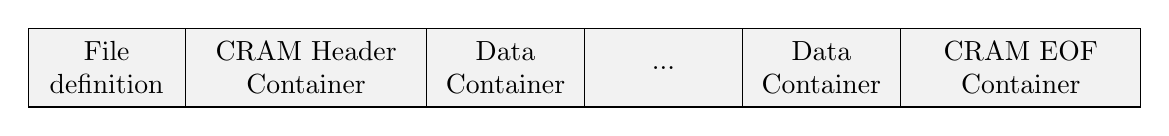
\begin{tikzpicture}[
  every node/.style={scale=1.0},
  boxes/.style={rectangle split,rectangle split parts=#1,draw,rectangle split horizontal,text width=5em,align=center,minimum height=1cm,fill=black!5,on grid},
  notes/.style={text width=20em,align=center,minimum height=1cm,on grid},
]
\node (file) [boxes=6] {
\nodepart{one}File definition
\nodepart[text width=8em]{two}CRAM Header Container
\nodepart{three}Data Container
\nodepart{four}...
\nodepart{five}Data Container
\nodepart[text width=8em]{six}CRAM EOF Container
};
\end{tikzpicture}

Figure 1: A CRAM file consists of a file definition, followed by a header container, then other containers.
\end{center}

Containers consist of one or more blocks. The first container, called the CRAM header container,
is used to store a textual header as described in the SAM specification (see the section 7.1).

\begin{center}
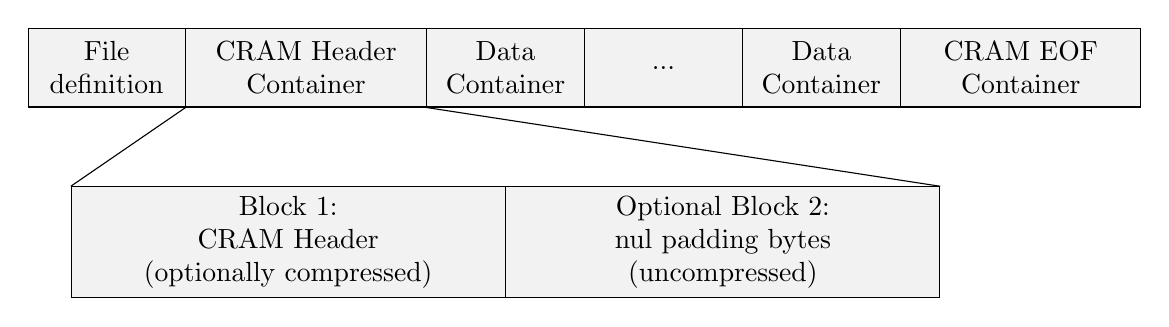
\begin{tikzpicture}[
  every node/.style={scale=1.0},
  boxes/.style={rectangle split,rectangle split parts=#1,draw,rectangle split horizontal,text width=5em,align=center,minimum height=1cm,fill=black!5,on grid},
  notes/.style={text width=20em,align=center,minimum height=1cm,on grid},
]
\node (file) [boxes=6] {
\nodepart{one}File definition
\nodepart[text width=8em]{two}CRAM Header Container
\nodepart{three}Data Container
\nodepart{four}...
\nodepart{five}Data Container
\nodepart[text width=8em]{six}CRAM EOF Container
};

\node (header) [boxes=2,below=1 of file.three south, text width=15em] {
\nodepart{one}Block 1:\break
CRAM Header\break
(optionally compressed)
\nodepart{two}Optional Block 2:\break
nul padding bytes\break
(uncompressed)
};
\draw (file.one split south) to (header.north west);
\draw (file.two split south) to (header.north east);
\end{tikzpicture}

Figure 2: The the first container holds the CRAM header text.
\end{center}

Each container starts with a container header structure followed by
one or more blocks.
The first block in each container is the compression header block
giving details of how to decode data in subsequent blocks.
Each block starts with a block header structure followed by the block
data.

\begin{center}
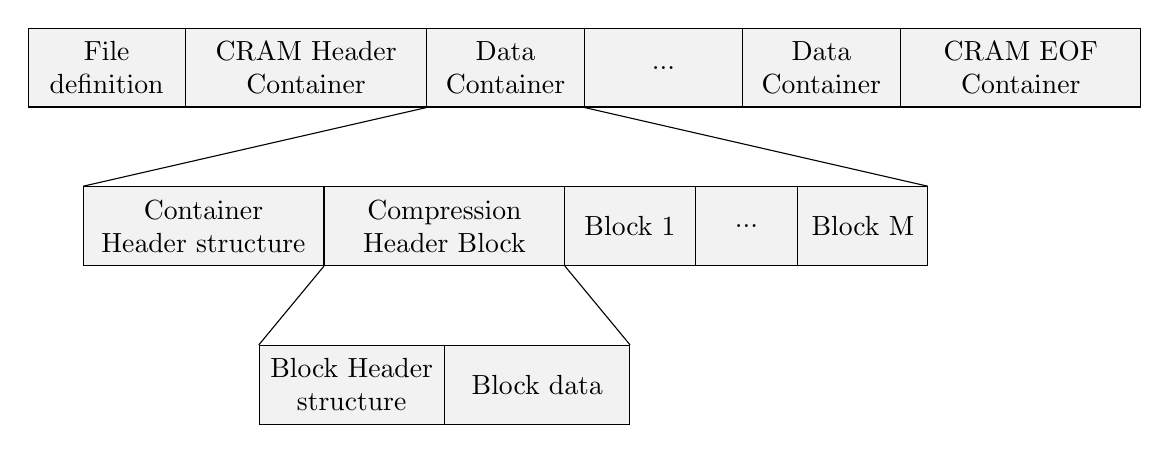
\begin{tikzpicture}[
  every node/.style={scale=1.0},
  boxes/.style={rectangle split,rectangle split parts=#1,draw,rectangle split horizontal,text width=5em,align=center,minimum height=1cm,fill=black!5,on grid},
  notes/.style={text width=20em,align=center,minimum height=1cm,on grid},
]
\node (file) [boxes=6] {
\nodepart{one}File definition
\nodepart[text width=8em]{two}CRAM Header Container
\nodepart{three}Data Container
\nodepart{four}...
\nodepart{five}Data Container
\nodepart[text width=8em]{six}CRAM EOF Container
};

\node (container) [boxes=5,below=1 of file.three south,text width=8em] {
\nodepart{one}Container Header structure
\nodepart{two}Compression Header Block
\nodepart[text width=4em]{three}Block 1
\nodepart[text width=3em]{four}...
\nodepart[text width=4em]{five}Block M
};
\draw (file.two split south) to (container.north west);
\draw (file.three split south) to (container.north east);

\node (blocks) [boxes=2,below=1 of container.two south,text width=6em] {
\nodepart{one}Block Header structure
\nodepart{two}Block data
};
\draw (container.one split south) to (blocks.north west);
\draw (container.two split south) to (blocks.north east);
\end{tikzpicture}

Figure 3: Containers as a series of blocks
\end{center}

The blocks after the compression header are organised logically into slices. One 
slice may contain, for example, a contiguous region of alignment data. Slices begin 
with a slice header block and are followed by one or more data blocks.
It is these data blocks which hold the primary bulk of CRAM data.
The data blocks are further subdivided into a core data block and one or more external data blocks.

\begin{center}
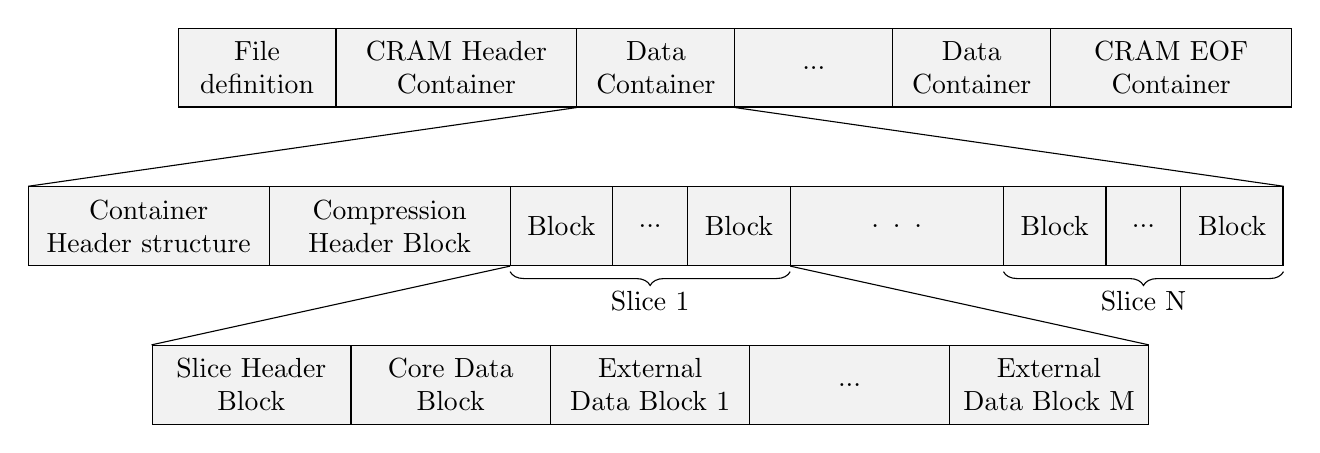
\begin{tikzpicture}[
  every node/.style={scale=1.0},
  boxes/.style={rectangle split,rectangle split parts=#1,draw,rectangle split horizontal,text width=5em,align=center,minimum height=1cm,fill=black!5,on grid},
  notes/.style={text width=20em,align=center,minimum height=1cm,on grid},
]
\node (file) [boxes=6] {
\nodepart{one}File definition
\nodepart[text width=8em]{two}CRAM Header Container
\nodepart{three}Data Container
\nodepart{four}...
\nodepart{five}Data Container
\nodepart[text width=8em]{six}CRAM EOF Container
};

\node (container) [boxes=9,below=1 of file.three south,text width=8em] {
\nodepart{one}Container Header structure
\nodepart{two}Compression Header Block
\nodepart[text width=3em]{three}Block
\nodepart[text width=2em]{four}...
\nodepart[text width=3em]{five}Block
\nodepart[text width=7em]{six}. . .
\nodepart[text width=3em]{seven}Block
\nodepart[text width=2em]{eight}...
\nodepart[text width=3em]{nine}Block
};
\draw (file.two split south) to (container.north west);
\draw (file.three split south) to (container.north east);

\draw[decoration={brace,mirror,amplitude=5pt,raise=2pt},decorate]
  (container.two split south) to (container.five split south);
\node [below=0.2 of container.four south] {Slice 1};

\draw[decoration={brace,mirror,amplitude=5pt,raise=2pt},decorate]
  (container.six split south) to (container.south east);
\node [below=0.2 of container.eight south] {Slice N};

\node (slice) [boxes=5,below=1 of container.four south, text width=6.5em] {
\nodepart{one}Slice Header Block
\nodepart{two}Core Data Block
\nodepart{three}External Data Block 1
\nodepart{four}...
\nodepart{five}External Data Block M
};
\draw (container.two split south) to (slice.north west);
\draw (container.five split south) to (slice.north east);
\end{tikzpicture}

Figure 4: Slices formed from a series of concatenated blocks
\end{center}

\section{\textbf{File definition}}

Each CRAM file starts with a fixed length (26 bytes) definition with the following 
fields:

\begin{tabular}{|l|l|l|}
\hline
\textbf{Data type} & \textbf{Name} & \textbf{Value}\tabularnewline
\hline
byte[4] & format magic number & CRAM (0x43 0x52 0x41 0x4d)\tabularnewline
\hline
unsigned byte & major format number & 3 (0x3)\tabularnewline
\hline
unsigned byte & minor format number & 1 (0x1)\tabularnewline
\hline
byte[20] & file id & CRAM file identifier (e.g. file name or SHA1 checksum)\tabularnewline
\hline
\end{tabular}

Valid CRAM \textit{major}.\textit{minor} version numbers are as follows:

\begin{itemize}
\item[\textit{1.0}]
The original public CRAM release.

\item[\textit{2.0}]
The first CRAM release implemented in both Java and C; tidied up
implementation vs specification differences in \textit{1.0}.

\item[\textit{2.1}]
Gained end of file markers; compatible with \textit{2.0}.

\item[\textit{3.0}]
Additional compression methods; header and data checksums;
improvements for unsorted data.

\item[\textit{3.1}]
Additional EXTERNAL compression codecs only.
\end {itemize}

CRAM 3.0 and 3.1 differ only in the list of compression
methods available, so tools that output CRAM 3 without using any 3.1
codecs should write the header to indicate 3.0 in order to permit
maximum compatibility.

\section{\textbf{Container header structure}}
\label{sec:container}

The file definition is followed by one or more containers with the following header 
structure where the container content is stored in the `blocks' field:

\begin{tabular}{|l|>{\raggedright}p{120pt}|>{\raggedright}p{260pt}|}
\hline
\textbf{Data type} & \textbf{Name} & \textbf{Value}
\tabularnewline
\hline
int32 & length & the sum of the lengths of all blocks in this container (headers and data); 
equal to the total byte length of the container minus the byte length of this header structure\tabularnewline
\hline
itf8 & reference sequence id & reference sequence identifier  or\linebreak{}
-1 for unmapped reads\linebreak{}
-2 for multiple reference sequences.\linebreak{}
All slices in this container must have a reference sequence id matching this value.\tabularnewline
\hline
itf8 & starting position on the reference & the alignment start position\tabularnewline
\hline
itf8 & alignment span & the length of the alignment\tabularnewline
\hline
itf8 & number of records & number of records in the container\tabularnewline
\hline
ltf8 & record counter & 1-based sequential index of records in the file/stream.\tabularnewline
\hline
ltf8 & bases & number of read bases\tabularnewline
\hline
itf8 & number of blocks & the total number of blocks in this container\tabularnewline
\hline
array\texttt{<}itf8\texttt{>} & landmarks & the locations of slices in this container as byte offsets from the end of
this container header, used for random access indexing.
For sequence data containers, the landmark count must equal the slice count.\linebreak{}
Since the block before the first slice is the compression header,
landmarks[0] is equal to the byte length of the compression header.\tabularnewline
\hline
int & crc32 & CRC32 hash of the all the preceding bytes in the container.\tabularnewline
\hline
byte[ ] & blocks & The blocks contained within the container.\tabularnewline
\hline
\end{tabular}

In the initial CRAM header container, the reference sequence id,
starting position on the reference, and alignment span fields must be
ignored when reading. The landmarks array is optional for the CRAM
header, but if it exists it should point to block offsets instead of
slices, with the first block containing the textual header.

In data containers specifying unmapped reads or multiple reference
sequences (i.e. reference sequence id $< 0$), the starting position on
the reference and alignment span fields must be ignored when
reading. When writing, it is recommended to set each of these ignored
fields to the value 0.


\subsection{\textbf{CRAM header container}}
\label{subsec:cram-header-container}

The first container in a CRAM file contains a textual header in one or more blocks.  See section~\ref{subsec:header-block} for more details on the layout of data within these blocks and constraints applied to the contents of the SAM header.

The landmarks field of the container header structure may be used to
indicate the offsets of the blocks used in the header container.
These may optionally be omitted by specifying an array size of zero.

\section{\textbf{Block structure}}
\label{sec:block-struct}

Containers consist of one or more blocks. Block compression is applied independently 
and in addition to any encodings used to compress data within the block. The block 
have the following header structure with the data stored in the `block data' field:

\begin{tabular}{|l|>{\raggedright}p{120pt}|>{\raggedright}p{260pt}|}
\hline
\textbf{Data type} & \textbf{Name} & \textbf{Value}
\tabularnewline
\hline
byte & method & the block compression method (and first CRAM version): \linebreak{}
0: raw (none)*\linebreak{}
1: gzip\linebreak{}
2: bzip2 (v2.0)\linebreak{}
3: lzma (v3.0)\linebreak{}
4: rans4x8 (v3.0)\linebreak{}
5: rans4x16 (v3.1)\linebreak{}
6: adaptive arithmetic coder (v3.1)\linebreak{}
7: fqzcomp (v3.1)\linebreak{}
8: name tokeniser (v3.1)
\tabularnewline
\hline
byte & block content type id & the block content type identifier\tabularnewline
\hline
itf8 & block content id & the block content identifier used to associate external 
data blocks with data series\tabularnewline
\hline
itf8 & size in bytes* & size of the block data after applying block compression\tabularnewline
\hline
itf8 & raw size in bytes* & size of the block data before applying block compression\tabularnewline
\hline
byte[ ] & block data & the data stored in the block:\linebreak{}
$\bullet$ bit stream of CRAM records (core data block)\linebreak{}
$\bullet$ byte stream (external data block)\linebreak{}
$\bullet$ additional fields ( header blocks)\tabularnewline
\hline
byte[4] & CRC32 & CRC32 hash value for all preceding bytes in the block\tabularnewline
\hline
\end{tabular}

* Note on raw method: both compressed and raw sizes must be set to the same value.

Empty blocks may occur in the files.
Blocks with a raw (uncompressed) size of zero are treated as empty,
irrespective of their ``method'' byte.  This is equivalent to
interpreting them as having method zero (raw) and compressed size of
zero.

\subsection{\textbf{Block content types}}

CRAM has the following block content types:

\begin{threeparttable}[t]
\begin{tabular}{|>{\raggedright}p{143pt}|>{\raggedright}p{45pt}|>{\raggedright}p{116pt}|>{\raggedright}p{114pt}|}
\hline
\textbf{Block content type} & \textbf{Block content type id} & \textbf{Name} & \textbf{Contents}\tabularnewline
\hline
FILE\_HEADER & 0 & CRAM header block & CRAM header\tabularnewline
\hline
COMPRESSION\_HEADER & 1 & Compression header block & See specific section\tabularnewline
\hline
SLICE\_HEADER\tnote{a} & 2 & Slice header block & See specific section\tabularnewline
\hline
 & 3 &  & reserved\tabularnewline
\hline
EXTERNAL\_DATA & 4 & external data block & data produced by external encodings\tabularnewline
\hline
CORE\_DATA & 5 & core data block & bit stream of all encodings except for external encodings\tabularnewline
\hline
\end{tabular}
\begin{tablenotes}
\item[a] Formerly MAPPED\_SLICE\_HEADER.  Now used by all slice headers regardless of mapping status.
\end{tablenotes}
\end{threeparttable}

\subsection{\textbf{Block content id}}

Block content id is used to distinguish between external blocks in the same slice. 
Each external encoding has an id parameter which must be one of the external block 
content ids. For external blocks the content id is a positive integer. For all 
other blocks content id should be 0. Consequently, all external encodings must 
not use content id less than 1. 

\subsubsection*{Data blocks}

Data is stored in data blocks. There are two types of data blocks: core data blocks 
and external data blocks.The difference between core and external data blocks is 
that core data blocks consist of data series that are compressed using bit encodings 
while the external data blocks are byte compressed. One core data block and any 
number of external data blocks are associated with each slice.

Writing to and reading from core and external data blocks is organised through 
CRAM records. Each data series is associated with an encoding. In case of external 
encodings the block content id is used to identify the block where the data series 
is stored. Please note that external blocks can have multiple data series associated 
with them; in this case the values from these data series will be interleaved. 


\subsection{\textbf{CRAM header block(s)}}
\label{subsec:header-block}

The SAM header is stored in the first block of the CRAM header container (see section~\ref{subsec:cram-header-container}).
This block may be uncompressed or gzip compressed only.
This block is followed by zero or more uncompressed expansion blocks.
If present, these permit in-place editing of the CRAM header, allowing it to grow or shrink with a compensatory size change applied to the subsequence expansion block, avoiding the need to rewrite the remainder of the file.
The contents of any expansion blocks should be zero bytes (nul characters).

The format of the initial SAM header block is a 32-bit little-endian integer holding the length of the text of the SAM header, minus nul-termination bytes, followed by the text itself.
Although 32-bit, the maximum permitted value is $2^{31}$, and all lengths must be positive.

The following constraints apply to the SAM header text: 

\begin{itemize}
\item The SQ:MD5 checksum is required unless the reference sequence has been embedded 
into the file.
\end{itemize}

\subsection{\textbf{Compression header block}}
\label{subsec:compression-header}

The compression header block consists of 3 parts: preservation map, data series 
encoding map and tag encoding map.

\subsubsection*{Preservation map}

The preservation map contains information about which data was preserved in the 
CRAM file. It is stored as a map with byte[2] keys:

\begin{tabular}{|l|l|>{\raggedright}p{100pt}|>{\raggedright}p{220pt}|}
\hline
\textbf{Key} & \textbf{Value data type} & \textbf{Name} & \textbf{Value}\tabularnewline
\hline
RN & bool & read names included & true if read names are preserved for all reads\tabularnewline
\hline
AP & bool & AP data series delta & true if AP data series is delta, false otherwise\tabularnewline
\hline
RR & bool & reference required & true if reference sequence is required to restore 
the data completely\tabularnewline
\hline
SM & byte[5] & substitution matrix & substitution matrix\tabularnewline
\hline
TD & array\texttt{<}byte\texttt{>} & tag ids dictionary & a list of lists of tag ids, see tag encoding section\tabularnewline
\hline
\end{tabular}

The boolean values are optional, defaulting to true when absent, although it is recommended to explicitly set them.  SM and TD are mandatory.

\subsubsection*{Data series encodings}

Each data series has an encoding. These encoding are stored in a map with byte[2] 
keys and are decoded in approximately this order\footnote{The precise order is defined in section~\ref{sec:record}.}:

\begin{threeparttable}[t]
\begin{tabular}{|l|l|>{\raggedright}p{100pt}|>{\raggedright}p{220pt}|}
\hline
\textbf{Key} & \textbf{Value data type} & \textbf{Name} & \textbf{Value}\tabularnewline
\hline
BF & encoding\texttt{<}int\texttt{>} & BAM bit flags & see separate section\tabularnewline
\hline
CF & encoding\texttt{<}int\texttt{>} & CRAM bit flags & see specific section\tabularnewline
\hline
RI & encoding\texttt{<}int\texttt{>} & reference id & record reference id from
the SAM file header\tabularnewline
\hline
RL & encoding\texttt{<}int\texttt{>} & read lengths & read lengths\tabularnewline
\hline
AP & encoding\texttt{<}int\texttt{>} & in-seq positions & if \textbf{AP-Delta} = true: 0-based alignment start
delta from the AP value in the previous record.
Note this delta may be negative, for example when switching references in a multi-reference slice.
When the record is the first in the slice, the previous position used is the slice alignment-start field (hence the first delta should be zero for single-reference slices, or the AP value itself for multi-reference slices).  \linebreak{}
if \textbf{AP-Delta} = false: encodes the alignment start position directly\tabularnewline
\hline
RG & encoding\texttt{<}int\texttt{>} & read groups & read groups. Special value 
`-1' stands for no group.\tabularnewline
\hline
RN\tnote{a} & encoding\texttt{<}byte[ ]\texttt{>} & read names & read names\tabularnewline
\hline
MF & encoding\texttt{<}int\texttt{>} & next mate bit flags & see specific section\tabularnewline
\hline
NS & encoding\texttt{<}int\texttt{>} & next fragment reference sequence id & reference 
sequence ids for the next fragment \tabularnewline
\hline
NP & encoding\texttt{<}int\texttt{>} & next mate alignment start & alignment positions 
for the next fragment\tabularnewline
\hline
TS & encoding\texttt{<}int\texttt{>} & template size & template sizes\tabularnewline
\hline
NF & encoding\texttt{<}int\texttt{>} & distance to next fragment & number of records
to skip to the next fragment\tnote{b}\tabularnewline
\hline
TL\tnote{c} & encoding\texttt{<}int\texttt{>} & tag ids  & list of tag ids, see tag encoding
section\tabularnewline
\hline
FN & encoding\texttt{<}int\texttt{>} & number of read features & number of read
features in each record\tabularnewline
\hline
FC & encoding\texttt{<}byte\texttt{>} & read features codes & see separate section\tabularnewline
\hline
FP & encoding\texttt{<}int\texttt{>} & in-read positions & positions of the read
features\tabularnewline
\hline
DL & encoding\texttt{<}int\texttt{>} & deletion lengths & base-pair deletion lengths\tabularnewline
\hline
BB & encoding\texttt{<}byte[ ]\texttt{>} & stretches of bases & bases\tabularnewline
\hline
QQ & encoding\texttt{<}byte[ ]\texttt{>} & stretches of quality scores & quality scores\tabularnewline
\hline
BS & encoding\texttt{<}byte\texttt{>} & base substitution codes & base substitution
codes\tabularnewline
\hline
IN & encoding\texttt{<}byte[ ]\texttt{>} & insertion & inserted bases\tabularnewline
\hline
RS & encoding\texttt{<}int\texttt{>} & reference skip length & number of skipped 
bases for the `N' read feature\tabularnewline
\hline
PD & encoding\texttt{<}int\texttt{>} & padding & number of padded bases\tabularnewline
\hline
HC & encoding\texttt{<}int\texttt{>} & hard clip & number of hard clipped bases\tabularnewline
\hline
SC & encoding\texttt{<}byte[ ]\texttt{>} & soft clip & soft clipped bases\tabularnewline
\hline
MQ & encoding\texttt{<}int\texttt{>} & mapping qualities & mapping quality scores\tabularnewline
\hline
BA & encoding\texttt{<}byte\texttt{>} & bases & bases\tabularnewline
\hline
QS & encoding\texttt{<}byte\texttt{>} & quality scores & quality scores\tabularnewline
\hline
TC\tnote{d} & N/A & legacy field & to be ignored\tabularnewline
\hline
TN\tnote{d} & N/A & legacy field & to be ignored\tabularnewline
\end{tabular}

\begin{tablenotes}
\item[a] Note RN this is decoded after MF if the record is detached from the mate and we are attempting to auto-generate read names.
\item[b] The count is reset for each slice so NF can only refer to a record later within this slice.
\item[c] TL is followed by decoding the tag values themselves, in order of appearance in the tag dictionary.
\item[d] TC and TN are legacy data series from CRAM 1.0.
They have no function in CRAM 3.0 and should not be present.
However some implementations do output them and decoders must silently skip these fields.
It is illegal for TC and TN to contain any data values, although there
may be empty blocks associated with them.
\end{tablenotes}
\end{threeparttable}

\subsubsection*{Tag encodings}
\label{subsubsec:tags}

The tag dictionary (TD) describes the unique combinations of tag id / type that occur on each alignment record.
For example if we search the id / types present in each record and find only two combinations -- X1:i BC:Z SA:Z: and X1:i: BC:Z -- then we have two dictionary entries in the TD map.

Let $L_{i}=\{T_{i0}, T_{i1}, \ldots, T_{ix}\}$ be a list of all tag ids for a record $R_{i}$, where $i$ is the sequential record index and $T_{ij}$ denotes $j$-th tag id in the record.
The list of unique $L_{i}$ is stored as the TD value in the preservation map.
Maintaining the order is not a requirement for encoders (hence ``combinations''), but it is permissible and thus different permutations, each encoded with their own elements in TD, should be supported by the decoder.
Each $L_{i}$ element in TD is assigned a sequential integer number starting with 0.
These integer numbers are referred to by the TL data series.
Using TD, an integer from the TL data series can be mapped back into a list of tag ids.
Thus per alignment record we only need to store tag values and not their ids and types.

The TD is written as a byte array consisting of $L_{i}$ values separated with \textbackslash{}0.
Each $L_{i}$ value is written as a concatenation of 3 byte $T_{ij}$ elements: tag id followed by BAM tag type code (one of A, c, C, s, S, i, I, f, F, Z, H or B, as described in the SAM specification).
For example the TD for tag lists X1:i BC:Z SA:Z and X1:i BC:Z may be encoded as X1CBCZSAZ\textbackslash{}0X1CBCZ\textbackslash{}0, with X1C indicating a 1 byte unsigned value for tag X1.

\subsubsection*{Tag values}

The encodings used for different tags are stored in a map.
The key is 3 bytes formed from the BAM tag id and type code, matching the TD dictionary described above.
Unlike the Data Series Encoding Map, the key is stored in the map as an ITF8 encoded integer, constructed using $(char1<<16) + (char2<<8) + type$.
For example, the 3-byte representation of OQ:Z is \{0x4F, 0x51, 0x5A\} and these bytes are interpreted as the integer key 0x004F515A, leading to an ITF8 byte stream \{0xE0, 0x4F, 0x51, 0x5A\}.

\begin{tabular}{|l|l|l|>{\raggedright}p{160pt}|}
\hline
\textbf{Key} & \textbf{Value data type} & \textbf{Name} & \textbf{Value}
\tabularnewline
\hline
TAG ID 1:TAG TYPE 1 & encoding\texttt{<}byte[ ]\texttt{>} & read tag 1 & tag values
(names and types are available in the data series code)\tabularnewline
\hline
... &  & ... & ...\tabularnewline
\hline
TAG ID N:TAG TYPE N & encoding\texttt{<}byte[ ]\texttt{>} & read tag N & ...\tabularnewline
\hline
\end{tabular}

Note that tag values are encoded as array of bytes. The routines to convert tag 
values into byte array and back are the same as in BAM with the exception of value 
type being captured in the tag key rather in the value.
Hence consuming 1 byte for types `C' and `c', 2 bytes for types `S' and `s', 4 bytes for types `I', `i' and `f', and a variable number of bytes for types `H', `Z' and `B'.

\subsection{\textbf{Slice header block}}

The slice header block is never compressed (block method=raw). For reference mapped 
reads the slice header also defines the reference sequence context of the data 
blocks associated with the slice. Mapped reads can be stored along with
\textbf{placed unmapped}\footnote{Unmapped reads can be \textit{placed} or \textit{unplaced}.
By placed unmapped read we mean a read that is unmapped according to bit 0x4 of the
BF (BAM bit flags) data series, but has position fields filled in, thus "placing"  it on a reference sequence. In contrast,
unplaced unmapped reads have have a reference sequence ID of -1 and alignment position of 0.}
reads on the same reference within the same slice.

Slices with the Multiple Reference flag (-2) set as the sequence ID in the header may contain reads
mapped to multiple external references, including unmapped\footnotemark[\value{footnote}] reads (placed on these references or unplaced),
but multiple embedded references cannot be combined in this way.  When multiple references are
used, the RI data series will be used to determine the reference sequence ID for each record.  This
data series is not present when only a single reference is used within a slice.

The Unmapped (-1) sequence ID in the header is for slices containing only unplaced
unmapped\footnotemark[\value{footnote}] reads.

A slice containing data that does not use the external reference in
any sequence may set the reference MD5 sum to zero.  This can happen
because the data is unmapped or the sequence has been stored verbatim
instead of via reference-differencing.  This latter scenario is
recommended for unsorted or non-coordinate-sorted data.

The slice header block contains the following fields.

\begin{tabular}{|l|l|>{\raggedright}p{200pt}|}
\hline
\textbf{Data type} & \textbf{Name} & \textbf{Value}\tabularnewline
\hline
itf8 & reference sequence id & reference sequence identifier or\linebreak{}
-1 for unmapped reads\linebreak{}
-2 for multiple reference sequences.\linebreak{}
This value must match that of its enclosing container.\tabularnewline
\hline
itf8 & alignment start & the alignment start position\tabularnewline
\hline
itf8 & alignment span & the length of the alignment\tabularnewline
\hline
itf8 & number of records & the number of records in the slice\tabularnewline
\hline
ltf8 & record counter & 1-based sequential index of records in the file/stream\tabularnewline
\hline
itf8 & number of blocks & the number of blocks in the slice\tabularnewline
\hline
itf8[ ] & block content ids & block content ids of the blocks in the slice\tabularnewline
\hline
itf8 & embedded reference bases block content id & block content id for the embedded 
reference sequence bases or -1 for none\tabularnewline
\hline
byte[16] & reference md5 & MD5 checksum of the reference bases within the slice 
boundaries.  If this slice has reference sequence id of -1 (unmapped) or -2 (multi-ref)
the MD5 should be 16 bytes of \textbackslash{}0. For embedded references, the MD5
can either be all-zeros or the MD5 of the embedded sequence.\tabularnewline
\hline
byte[ ] & optional tags & a series of tag,type,value tuples encoded as
per BAM auxiliary fields.\tabularnewline
\hline
\end{tabular}

The alignment start and alignment span values should only be utilised
during decoding if the slice has mapped data aligned to a single
reference (reference sequence id $>= 0$).  For multi-reference slices
or those with unmapped data, it is recommended to fill these fields
with value 0.

The optional tags are encoded in the same manner as BAM tags.  I.e. a
series of binary encoded tags concatenated together where each tag
consists of a 2 byte key (matching [A-Za-z][A-Za-z0-9]) followed by a
1 byte type ([AfZHcCsSiIB]) followed by a string of bytes in a format
defined by the type.

Tags starting in a capital letter are reserved while lowercase ones or
those starting with X, Y or Z are user definable.  Any tag not
understood by a decoder should be skipped over without producing an
error.

At present no tags are defined.

% Details omitted until we fully work through all the corner cases,
% such as seq/qual of *.
%
% Reserved tags are defined as follows:
% 
% \begin{tabular}{|l|l|>{\raggedright}p{325pt}|}
% \hline
% \textbf{Tag type} & \textbf{BAM format} & \textbf{Meaning}\tabularnewline
% \hline
% BD & i & Sum over all reads of the CRC32 hash of sequence base.  This
% may be used to validate round-trips in and out of CRAM.
% calls\tabularnewline
% \hline
% SD & i & Sum over all reads of the CRC32 hash of quality scores. (If
% the quality string is ``*'' in SAM then the hash is of the BAM encoded
% version - a string of bytes with value 255.)\tabularnewline
% \hline
% \end{tabular}


\subsection{\textbf{Core data block}}

A core data block is a bit stream (most significant bit first) consisting of data from one 
or more CRAM records. Please note that one byte could hold more then one CRAM record 
as a minimal CRAM record could be just a few bits long. The core data block has 
the following fields:

\begin{tabular}{|l|>{\raggedright}p{120pt}|>{\raggedright}p{260pt}|}
\hline
\textbf{Data type} & \textbf{Name} & \textbf{Value}
\tabularnewline
\hline
bit[ ] & CRAM record 1 & The first CRAM record\tabularnewline
\hline
... & ... & ...\tabularnewline
\hline
bit[ ] & CRAM record N & The Nth CRAM record \tabularnewline
\hline
\end{tabular}

\subsection{\textbf{External data blocks}}

The relationship between the core data block and external data blocks is shown in the following 
picture: 

\begin{center}
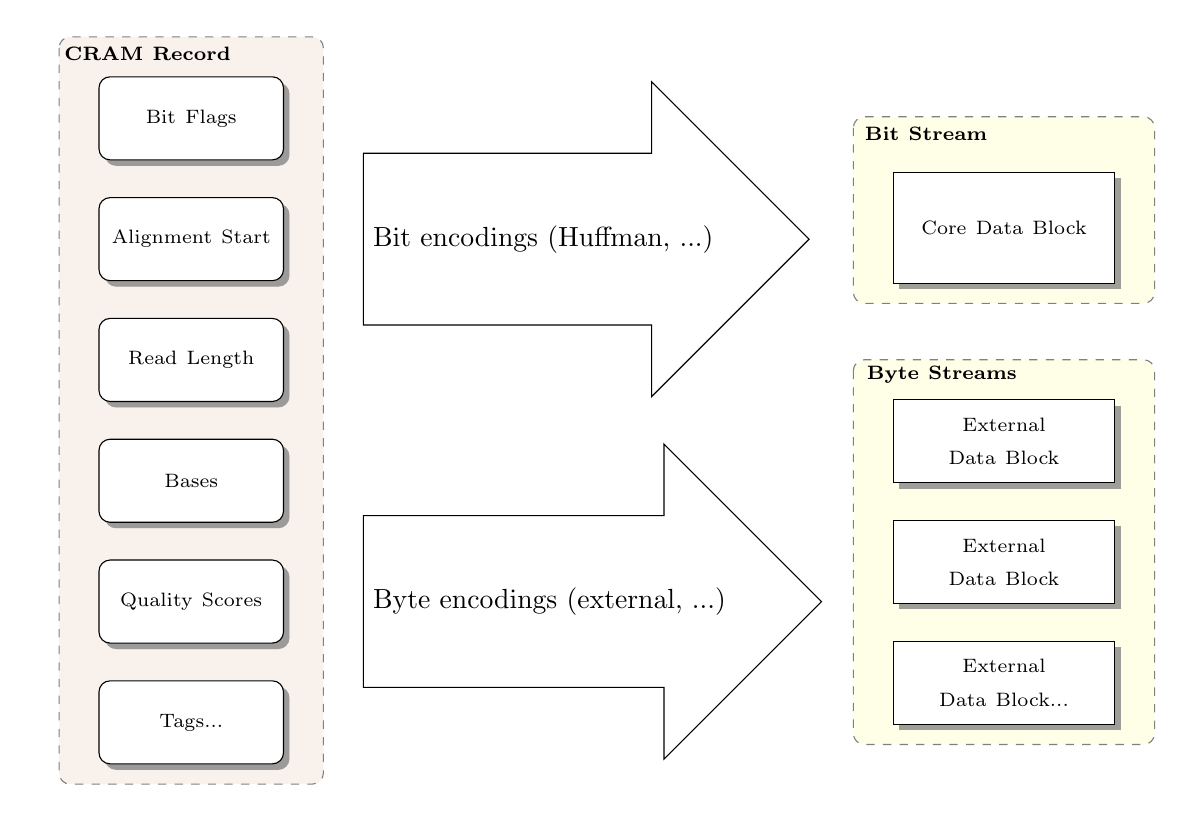
\begin{tikzpicture}

\usetikzlibrary{shapes, shadows, positioning, arrows,  decorations.markings}

\pgfdeclarelayer{background}
\pgfsetlayers{background,main}

\tikzstyle{dsbox} = [blockbox, text width=6em, minimum width=6em, minimum height=3em, rounded corners, drop shadow]
\tikzstyle{blockbox}=[draw, fill=white, text width=4.0em, text centered, minimum height=1.0em, drop shadow]
\tikzstyle{encodedblocklarge} = [blockbox, text width=6em, minimum width=8em, minimum height=4em, drop shadow]
\tikzstyle{encodedblock} = [blockbox, text width=6em, minimum width=8em, minimum height=3em, drop shadow]

\tikzstyle{texto} = [above, text width=8em, text centered]

\newcommand{\cramRecord}[6]{%
\begin{pgfonlayer}{background}
    \path (#1.west |- #1.north) + (-0.5, 0.5) node (a1) {};
    \path (#1.east |- #6.south) + (+0.5,-0.25) node (a2) {};
    \path[fill=brown!10,rounded corners, draw=black!50, dashed]
      (a1) rectangle (a2);
    \path (a1.east |- a1.south) + (1.0,-0.3) node[texto]
      {\scriptsize\textbf{CRAM Record}};
\end{pgfonlayer}}

\newcommand{\dsbox}[2]{node (p#1) [dsbox]
{\scriptsize{#2}}}
\newcommand{\encodedblock}[2]{node (p#1) [encodedblock]
	{\scriptsize{#2}}}
\newcommand{\encodedblocklarge}[2]{node (p#1) [encodedblocklarge]
   {\scriptsize{#2}}}

\path +(-2.5,-1.5) \dsbox{1}{Bit Flags};
\path (p1.south)+(0.0,-1.0) \dsbox{2}{Alignment Start};
\path (p2.south)+(0.0,-1.0) \dsbox{3}{Read Length};
\path (p3.south)+(0.0,-1.0) \dsbox{4}{Bases};
\path (p4.south)+(0.0,-1.0) \dsbox{5}{Quality Scores};
\path (p5.south)+(0.0,-1.0) \dsbox{6}{Tags...};

\cramRecord{p1}{p2}{p3}{p4}{p5}{p6}

\newcommand{\blockStreams}[4]{%
\begin{pgfonlayer}{background}
    \path (#1.west |- #1.north)+(-0.5, .7) node (a1) {};
    \path (#1.east |- #1.south)+(+0.5, -0.25) node (a2) {};
    \path (#2.west |- #2.north)+(-0.5, 0.5) node (a3) {};
    \path (#4.east |- #4.south)+(+0.5, -0.25) node (a4) {};
    \path[fill=yellow!10, rounded corners, draw=black!50, dashed]
      (a1) rectangle (a2);
    \path (a1.east |- a1.south)+(0.8,-0.3) node[texto]
      {\scriptsize\textbf{Bit Stream}};
    \path[fill=yellow!10, rounded corners, draw=black!50, dashed]
      (a3) rectangle (a4);
    \path (a3.east |- a3.south)+(1.0,-0.3) node[texto]{\scriptsize\textbf{Byte Streams}};
\end{pgfonlayer}}

\path (a1.south) + (12.0, -2.3) \encodedblocklarge {7} {Core Data Block};
\path (p7.south) + (0.0, -2.0) \encodedblock {8} {External Data Block};
\path (p8.south) + (0.0, -1.0) \encodedblock {9} {External Data Block}; 
\path (p9.south) + (0.0, -1.0) \encodedblock {10}{External Data Block...};

\blockStreams {p7} {p8} {p9} {p10}

\node[minimum size=4cm, right = of p2, single arrow, draw, single arrow head indent=0ex, black] {Bit encodings (Huffman, ...) };

\node[minimum size=4cm, right = of p5, single arrow, draw, single arrow head indent=0ex, black] {Byte encodings (external, ...) };

\end{tikzpicture}

Figure 5: The relationship between core and external encodings, and core and external data blocks.

\end{center}

The picture shows how a CRAM record (on the left) is distributed between the core 
data block and one or more external data blocks, via core or external encodings. The specific 
encodings presented are only examples for purposes of illustration. The main point is 
to distinguish between core bit encodings whose output is always stored in a core data 
block, and external byte encodings whose output is always stored in external data 
blocks.

\section{\textbf{End of file container}}

A special container is used to mark the end of a file or stream. It is required in version 3 or later. The idea is to provide an easy and a quick way to detect that a CRAM file or stream is complete. The marker is basically an empty container with ref seq id set to -1 (unaligned) and alignment 
start set to 4542278.

Here is a complete content of the EOF container explained in detail:

\begin{tabular}{|l|l|>{\raggedright}p{150pt}|>{\raggedright}p{180pt}|}
\hline
\textbf{hex bytes} & \textbf{data type} & \textbf{decimal value} & \textbf{field 
name}\tabularnewline
\hline
\multicolumn{4}{|l|}{\textit{Container header}}\tabularnewline
\hline
0f 00 00 00 & integer & 15 & size of blocks data\tabularnewline
\hline
ff ff ff ff 0f & itf8 & -1 & ref seq id\tabularnewline
\hline
e0 45 4f 46 & itf8 & 4542278 & alignment start\tabularnewline
\hline
00 & itf8 & 0 & alignment span\tabularnewline
\hline
00 & itf8 & 0 & number of records\tabularnewline
\hline
00 & itf8 & 0 & global record counter\tabularnewline
\hline
00 & itf8 & 0 & bases\tabularnewline
\hline
01 & itf8 & 1 & block count\tabularnewline
\hline
00 & array & 0 & landmarks\tabularnewline
\hline
05 bd d9 4f & integer & 1339669765 & container header CRC32\tabularnewline
\hline
\multicolumn{4}{|l|}{\textit{Compression header block}}\tabularnewline
\hline
00 & byte & 0 (RAW) & compression method\tabularnewline
\hline
01 & byte & 1 (COMPRESSION\_HEADER) & block content type\tabularnewline
\hline
00 & itf8 & 0 & block content id\tabularnewline
\hline
06 & itf8 & 6 & compressed size\tabularnewline
\hline
06 & itf8 & 6 & uncompressed size\tabularnewline
\hline
\multicolumn{4}{|l|}{\textit{Compression header}}\tabularnewline
\hline
01 & itf8 & 1 & preservation map byte size\tabularnewline
\hline
00 & itf8 & 0 & preservation map size\tabularnewline
\hline
01 & itf8 & 1 & encoding map byte size\tabularnewline
\hline
00 & itf8 & 0 & encoding map size\tabularnewline
\hline
01 & itf8 & 1 & tag encoding byte size\tabularnewline
\hline
00 & itf8 & 0 & tag encoding map size\tabularnewline
\hline
ee 63 01 4b & integer & 1258382318 & block CRC32\tabularnewline
\hline
\end{tabular}

When compiled together the EOF marker is 38 bytes long and in hex representation 
is:

0f 00 00 00 ff ff ff ff 0f e0 45 4f 46 00 00 00 00 01 00 05 bd d9 4f 00 01 00 06 06 01 00 01 00 01 00 ee 63 01 4b

\section{\textbf{Record structure}}
\label{sec:record}

CRAM record is based on the SAM record but has additional features allowing for 
more efficient data storage.  In contrast to BAM record CRAM record uses bits as 
well as bytes for data storage. This way, for example, various coding techniques 
which output variable length binary codes can be used directly in CRAM. On the 
other hand, data series that do not require binary coding can be stored separately 
in external blocks with some other compression applied to them independently.

As CRAM data series may be interleaved within the same blocks\footnote{Interleaving can sometimes provide better compression, however it also adds dependency between types of data meaning it is not possible to selectively decode one data series if it co-locates with another data series in the same block.} understanding the order in which CRAM data series must be decoded is vital.

The overall flowchart is below, with more detailed description in the subsequent sections.

\algnewcommand\algorithmicto{\text{ \textbf{to} }}

\subsection{\textbf{CRAM record}}

Both mapped and unmapped reads start with the following fields. Please note that 
the data series type refers to the logical data type and the data series name corresponds 
to the data series encoding map.

\begin{tabular}{|>{\raggedright}p{70pt}|>{\raggedright}p{75pt}|>{\raggedright}p{90pt}|>{\raggedright}p{171pt}|}
\hline
\textbf{Data series type} & \textbf{Data series name} & \textbf{Field} & \textbf{Description}\tabularnewline
\hline
int & BF & BAM bit flags & see BAM bit flags below\tabularnewline
\hline
int & CF & CRAM bit flags & see CRAM bit flags below\tabularnewline
\hline
- & - & Positional data & See section \ref{subsec:positions}\tabularnewline
\hline
- & - & Read names & See section \ref{subsec:names}\tabularnewline
\hline
- & - & Mate records & See section \ref{subsec:mate}\tabularnewline
\hline
- & - & Auxiliary tags & See section \ref{subsec:tags}\tabularnewline
\hline
- & - & Sequences & See sections \ref{subsec:mapped} and \ref{subsec:unmapped}\tabularnewline
\hline
\end{tabular}

\subsubsection*{\textbf{BAM bit flags (BF data series)}}

The following flags are duplicated from the SAM and BAM specification, with identical meaning.
Note however some of these flags can be derived during decode, so may be omitted in the CRAM file and the bits computed based on both reads of a pair-end library residing within the same slice.

\begin{threeparttable}[t]
\begin{tabular}{|>{\raggedright}p{144pt}|>{\raggedright}p{144pt}|>{\raggedright}p{144pt}|}
\hline
\textbf{Bit flag} & \textbf{Comment} & \textbf{Description}\tabularnewline
\hline
0x1 &  & template having multiple segments in sequencing\tabularnewline
\hline
0x2 &  & each segment properly aligned according to the aligner\tabularnewline
\hline
0x4 &  & segment unmapped\tnote{a}\tabularnewline
\hline
0x8 & calculated\tnote{b}\ \ or stored in the mate's info & next segment in template unmapped\tabularnewline
\hline
0x10 &  & SEQ being reverse complemented\tabularnewline
\hline
0x20 & calculated\tnote{b}\ \ or stored in the mate's info & SEQ of the next segment in the
template being reverse complemented\tabularnewline
\hline
0x40 &  & the first segment in the template\tnote{c}\tabularnewline
\hline
0x80 &  & the last segment in the template\tnote{c}\tabularnewline
\hline
0x100 &  & secondary alignment\tabularnewline
\hline
0x200 &  & not passing quality controls\tabularnewline
\hline
0x400 &  & PCT or optical duplicate\tabularnewline
\hline
0x800 &  & Supplementary alignment\tabularnewline
\hline
\end{tabular}
\begin{tablenotes}
\item[a] Bit 0x4 is the only reliable place to tell whether the read is unmapped.  If 0x4 is set, no assumptions may be made about bits 0x2, 0x100 and 0x800.
\item[b] For segments within the same slice.
\item[c] Bits 0x40 and 0x80 reflect the read ordering within each template inherent in the sequencing technology used, which may be independent from the actual mapping orientation.
If 0x40 and 0x80 are both set, the read is part of a linear template (one where the template sequence is expected to be in a linear order), but it is neither the first nor the last read.
If both 0x40 and 0x80 are unset, the index of the read in the template is unknown.
This may happen for a non-linear template (such as one constructed by stitching together other templates) or when this information is lost during data processing.
\end{tablenotes}
\end{threeparttable}

\subsubsection*{\textbf{CRAM bit flags (CF data series)}}

The CRAM bit flags (also known as compression bit flags) expressed as an integer represent the CF data series. 
The following compression flags are defined for each CRAM read record:

\begin{tabular}{|>{\raggedright}p{39pt}|>{\raggedright}p{150pt}|>{\raggedright}p{242pt}|}
\hline
\textbf{Bit flag} & \textbf{Name} & \textbf{Description}\tabularnewline
\hline
0x1 & quality scores stored as array & quality scores can be stored as read features
or as an array similar to read bases.\tabularnewline
\hline
0x2 & detached & mate information is stored verbatim (e.g. because the pair spans multiple slices or the fields differ to the CRAM computed method)\tabularnewline
\hline
0x4 & has mate downstream & tells if the next segment should be expected further
in the stream\tabularnewline
\hline
0x8 & decode sequence as ``*'' & informs the decoder that the sequence
is unknown and that any encoded reference differences are present only to
recreate the CIGAR string.\tabularnewline
\hline
\end{tabular}


The following pseudocode describes the general process of decoding an entire CRAM record.
The sequence data itself is in one of two encoding formats depending on whether the record is aligned (mapped).

\subsubsection*{\textbf{Decode pseudocode}}
\newlength{\maxwidth}
\newcommand{\algalign}[2] % #1 = text to left, #2 = text to right
{\makebox[\maxwidth][l]{$#1{}$}${}#2$}

\begin{algorithmic}[1]
\Procedure{DecodeRecord}{}
\settowidth{\maxwidth}{CRAM\_flags\quad}
\State \algalign{BAM\_flags}{\gets}  \Call{ReadItem}{BF, Integer}
\State \algalign{CRAM\_flags}{\gets} \Call{ReadItem}{CF, Integer}
\State \Call{DecodePositions}{}\Comment{See section \ref{subsec:positions}}
\State \Call{DecodeNames}{}\Comment{See section \ref{subsec:names}}
\State \Call{DecodeMateData}{}\Comment{See section \ref{subsec:mate}}
\State \Call{DecodeTagData}{}\Comment{See section \ref{subsec:tags}}
\Statex

\If{$(BF$ AND $4) \ne 0$}\Comment{Unmapped flag}
  \State \Call{DecodeMappedRead}{}\Comment{See section \ref{subsec:mapped}}
\Else
  \State \Call{DecodeUnmappedRead}{}\Comment{See section \ref{subsec:unmapped}}
\EndIf
\EndProcedure
\end{algorithmic}

\subsection{\textbf{CRAM positional data}}
\label{subsec:positions}

Following the bit-wise BAM and CRAM flags, CRAM encodes positional related data including reference, alignment positions and length, and read-group.
Positional data is stored for both mapped and unmapped sequences, as unmapped data may still be ``placed'' at a specific location in the genome (without being aligned).
Typically this is done to keep a sequence pair (paired-end or mate-pair sequencing libraries) together when one of the pair aligns and the other does not.

For reads stored in a position-sorted slice, the AP-delta flag in the compression header preservation map should be set and the AP data series will be delta encoded, using the slice alignment-start value as the first position to delta against.
Note for multi-reference slices this may mean that the AP series includes negative values, such as when moving from an alignment to the end of one reference sequence to the start of the next or to unmapped unplaced data.  When the AP-delta flag is not set the AP data series is stored as a normal integer value.

\begin{tabular}{|>{\raggedright}p{70pt}|>{\raggedright}p{75pt}|>{\raggedright}p{90pt}|>{\raggedright}p{171pt}|}
\hline
\textbf{Data series type} & \textbf{Data series name} & \textbf{Field} & \textbf{Description}\tabularnewline
\hline
int & RI & ref id & reference sequence id (only present in multiref slices)\tabularnewline
\hline
int & RL & read length & the length of the read\tabularnewline
\hline
int & AP & alignment start & the alignment start position\tabularnewline
\hline
int & RG & read group & the read group identifier expressed as the N\textsuperscript{th} record in the header, starting from 0 with -1 for no group\tabularnewline
\hline
\end{tabular}

\vskip 20pt
\begin{algorithmic}[1]
\Procedure{DecodePositions}{}
\If{$slice\_header.reference\_sequence\_id = -2$}
  \State $reference\_id\gets$ \Call{ReadItem}{RI, Integer}
\Else
  \State $reference\_id\gets slice\_header.reference\_sequence\_id$
\EndIf
\State $read\_length \gets$ \Call{ReadItem}{RL, Integer}
\If{$container\_pmap.AP\_delta \ne 0$}
    \If{$first\_record\_in\_slice$}
        \State $last\_position\gets$ $slice\_header.alignment\_start$
    \EndIf
    \State $alignment\_position \gets$ \Call{ReadItem}{AP, Integer} + $last\_position$
    \State $last\_position \gets alignment\_position$
\Else
    \State $alignment\_position \gets$ \Call{ReadItem}{AP, Integer}
\EndIf
\State $read\_group \gets$ \Call{ReadItem}{RG, Integer}
\EndProcedure
\end{algorithmic}

\subsection{Read names (RN data series)}
\label{subsec:names}

Read names can be preserved in the CRAM format, but this is optional and is governed by the \texttt{RN} preservation map key in the container compression header. See section \ref{subsec:compression-header}.
When read names are not preserved the CRAM decoder should generate names, typically based on the file name and a numeric ID of the read using the record counter field of the slice header block.
Note read names may still be preserved even when the \texttt{RN} compression header key indicates otherwise, such as where a read is part of a read-pair and the pair spans multiple slices.
In this situation the record will be marked as detached (see the CF data series) and the mate data below (section \ref{subsec:mate}) will contain the read name.

\begin{tabular}{|>{\raggedright}p{70pt}|>{\raggedright}p{75pt}|>{\raggedright}p{90pt}|>{\raggedright}p{171pt}|}
\hline
\textbf{Data series type} & \textbf{Data series name} & \textbf{Field} & \textbf{Description}\tabularnewline
\hline
byte[ ] & RN & read names & read names\tabularnewline
\hline
\end{tabular}

\vskip 20pt
\begin{algorithmic}[1]
\Procedure{DecodeNames}{}
\If{$container\_pmap.read\_names\_included = 1$}
  \State $read\_name \gets$ \Call{ReadItem}{RN, Byte[]}
\Else
  \State $read\_name \gets$ \Call{GenerateName}{}
\EndIf
\Statex
\EndProcedure
\end{algorithmic}

\subsection{\textbf{Mate records}}
\label{subsec:mate}

There are two ways in which mate information can be preserved in CRAM.
If the next fragment is not in the same slice we store verbatim copies of the insert size, mate reference chromosome and positions, and mate flags (mapped status, orientation) for both records.
In this case both records are labelled as ``detached'' in the CF data series using bit 2.

If this and the next fragment are within the same slice, we can derive much of this information by comparing the two records.
The upstream record has CF bit 4 (mate downstream) flag set and stores the number of records to skip (in the NF data series) between this record and the record for the next fragment on this template, with zero meaning the next fragment is also the next record.
The downstream record has neither CF bits 2 (detached) or 4 (mate downstream) set nor does it use the NF data series (unless it also has an additional ``next fragment'' to refer to).

It is not mandatory to use this deduplication approach and optionally CRAM write implementations may wish to label data as detached even when all records for the template reside in the same slice.
One reason to do this may be to preserve inconsistent data so that it round-trips through the CRAM format with full fidelity

\begin{tabular}{|>{\raggedright}p{68pt}|>{\raggedright}p{115pt}|>{\raggedright}p{228pt}|}
\hline
\textbf{Data series type} & \textbf{Data series name} & \textbf{Description}\tabularnewline
\hline
int & NF & the number of records to skip to the next fragment\tabularnewline
\hline
\end{tabular}

In the above case, the NS (mate reference name), NP (mate position) and TS (template size) fields for both records should be derived once the mate has also been decoded.
Mate reference name and position are obvious and simply copied from the mate.
The template size is computed using the method described in the SAM specification; the inclusive distance from the leftmost to rightmost mapped bases with the sign being positive for the leftmost record and negative for the rightmost record.

If the next fragment is not found within this slice then the following structure is included into the CRAM record.
Note there are cases where read-pairs within the same slice may be marked as detached and use this structure, such as to store mate-pair information that does not match the algorithm used by CRAM for computing the mate data on-the-fly.

\begin{tabular}{|>{\raggedright}p{66pt}|>{\raggedright}p{117pt}|>{\raggedright}p{228pt}|}
\hline
\textbf{Data series type} & \textbf{Data series name} & \textbf{Description}\tabularnewline
\hline
int & MF & next mate bit flags, see table below\tabularnewline
\hline
byte[ ] & RN & the read name (if and only if not known already)\tabularnewline
\hline
int & NS & mate reference sequence identifier \tabularnewline
\hline
int & NP & mate alignment start position \tabularnewline
\hline
int & TS & the size of the template (insert size)\tabularnewline
\hline
\end{tabular}

\subsubsection*{Next mate bit flags (MF data series)}

The next mate bit flags expressed as an integer represent the MF data series.
These represent the missing bits we excluded from the BF data series (when compared to the full SAM/BAM flags).
The following bit flags are defined:

\begin{tabular}{|>{\raggedright}p{47pt}|>{\raggedright}p{134pt}|>{\raggedright}p{250pt}|}
\hline
\textbf{Bit flag} & \textbf{Name} & \textbf{Description}\tabularnewline
\hline
0x1 & mate negative strand bit & the bit is set if the mate is on the negative
strand\tabularnewline
\hline
0x2 & mate unmapped bit & the bit is set if the mate is unmapped\tabularnewline
\hline
\end{tabular}


\subsubsection*{\textbf{Decode mate pseudocode}}

In the following pseudocode we are assuming the current record is $this$ and its mate is $next\_frag$.

\begin{algorithmic}[1]
\Procedure{DecodeMateData}{}
\If{$CF$ AND $2$}\Comment{Detached from mate}
  \State $mate\_flags\gets $ \Call{ReadItem}{MF,Integer}
  \If{$mate\_flags$ AND 1}
    \State $bam\_flags\gets bam\_flags$\ OR\ 0x20\Comment{Mate is reverse-complemented}
  \EndIf
  \If{$mate\_flags$ AND 2}
    \State $bam\_flags\gets bam\_flags$\ OR\ 0x08\Comment{Mate is unmapped}
  \EndIf
  \If{$container\_pmap.read\_names\_included \ne 1$}
    \State $read\_name \gets$ \Call{ReadItem}{RN, Byte[]}
  \EndIf
\settowidth{\maxwidth}{mate\_position\ }
\State \algalign{mate\_ref\_id}{\gets}  \Call{ReadItem}{NS, Integer}
\State \algalign{mate\_position}{\gets} \Call{ReadItem}{NP, Integer}
\State \algalign{template\_size}{\gets} \Call{ReadItem}{TS, Integer}
\ElsIf{$CF$ AND $4$}\Comment{Mate is downstream}
  \If{$next\_frag.bam\_flags$ AND 0x10}
    \State $this.bam\_flags \gets this.bam\_flags$\ OR\ 0x20\Comment{next segment reverse complemented}
  \EndIf
  \If{$next\_frag.bam\_flags$ AND 0x04}
    \State $this.bam\_flags \gets this.bam\_flags$\ OR\ 0x08\Comment{next segment unmapped}
  \EndIf
  \State $next\_frag\gets$ \Call{ReadItem}{NF,Integer}
  \State $next\_record\gets this\_record + next\_frag + 1$
  \State Resolve $mate\_ref\_id$ for $this\_record$ and $next\_record$ once both have been decoded
  \State Resolve $mate\_position$ for $this\_record$ and $next\_record$ once both have been decoded
  \State Find leftmost and rightmost mapped coordinate in records $this\_record$ and $next\_record$.
  \State For leftmost of $this\_record$ and $next\_record$: $template\_size\gets rightmost-leftmost+1$
  \State For rightmost of $this\_record$ and $next\_record$: $template\_size\gets -(rightmost-leftmost+1)$
\EndIf
\EndProcedure
\end{algorithmic}

Note as with the SAM specification a template may be permitted to have more than two alignment records.
In this case the ``mate'' for each record is considered to be the next record, with the mate for the last record being the first to form a circular list.
The above algorithm is a simplification that does not deal with this scenario.
The full method needs to observe when record $this+NF$ is also labelled as having an additional mate downstream.
One recommended approach is to resolve the mate information in a second pass, once the entire slice has been decoded.
The final segment in the mate chain needs to set $bam\_flags$ fields 0x20 and 0x08 accordingly based on the first segment.
This is also not listed in the above algorithm, for brevity.

\subsection{Auxiliary tags}
\label{subsec:tags}

Tags are encoded using a tag line (TL data series) integer into the tag dictionary (TD field in the compression header preservation map, see section \ref{subsec:compression-header}).
See section \ref{subsubsec:tags} for a more detailed description of this process.

\begin{tabular}{|>{\raggedright}p{70pt}|>{\raggedright}p{75pt}|>{\raggedright}p{90pt}|>{\raggedright}p{200pt}|}
\hline
\textbf{Data series type} & \textbf{Data series name} & \textbf{Field} & \textbf{Description}\tabularnewline
\hline
int & TL & tag line & an index into the tag dictionary (TD)\tabularnewline
\hline
* & ??? & tag name/type & 3 character key (2 tag identifier and 1 tag type), as specified by the tag dictionary\tabularnewline
\hline
\end{tabular}

\vskip 20pt
\begin{algorithmic}[1]
\Procedure{DecodeTagData}{}
\State $tag\_line\gets$ \Call{ReadItem}{TL,Integer}
\ForAll {$ele \in container\_pmap.tag\_dict(tag\_line)$}
  \State $name\gets$ first two characters of $ele$
  \State $tag(type)\gets$ last character of $ele$
  \State $tag(name)\gets$ \Call{ReadItem}{$ele$, Byte[]}
\EndFor
\EndProcedure
\end{algorithmic}

In the above procedure, $name$ is a two letter tag name and $type$ is one of the permitted types documented in the SAM/BAM specification.
Type is \texttt{c} (signed 8-bit integer), \texttt{C} (unsigned 8-bit integer), \texttt{s} (signed 16-bit integer), \texttt{S} (unsigned 16-bit integer), \texttt{i} (signed 32-bit integer), \texttt{I} (unsigned 32-bit integer), \texttt{f} (32-bit float), \texttt{Z} (nul-terminated string), \texttt{H} (nul-terminated string of hex digits) and \texttt{B} (binary data in array format with the first byte being one of c,C,s,S,i,I,f using the meaning above, a 32-bit integer for the number of array elements, followed by array data encoded using the specified format).  All integers are little endian encoded.

For example a SAM tag \texttt{MQ:i} has name \texttt{MQ} and type \texttt{i} and will be decoded using one of MQc, MQC, MQs, MQS, MQi and MQI data series depending on size and sign of the integer value.

Note some auxiliary tags can be created automatically during decode so can optionally be removed by the encoder.
However if the decoder finds a tag stored verbatim it should use this in preference to automatically computing the value.

The RG (read group) auxiliary tag should be created if the read group (RG data series) value is not $-1$.

The MD and NM auxiliary tags store the differences (an edit string) between the sequence and the reference along with the number of mismatches.
These may optionally be created on-the-fly during reference-based sequence reconstruction and should match the description provided in the SAMtags document.
An encoder may decide to store these verbatim when no reference is used or where the automatically constructed values differ to the input data.

Note there is no mechanism to describe which records have MD/NM present and which do not.
If this is deemed important, the only recourse is to store all MD and NM verbatim and to request that the decoding software does not automatically generate its own for records that have no stored MD and NM tags.

\subsection{\textbf{Mapped reads}}
\label{subsec:mapped}

\subsubsection*{\textbf{Read feature records}}
\label{subsec:features}

Read features are used to store read details that are expressed using read coordinates 
(e.g. base differences respective to the reference sequence). The read feature 
records start with the number of read features followed by the read features themselves.
Finally the single mapping quality and per-base quality scores are stored.

\begin{threeparttable}[t]
\begin{tabular}{|>{\raggedright}p{88pt}|>{\raggedright}p{83pt}|>{\raggedright}p{85pt}|>{\raggedright}p{180pt}|}
\hline
\textbf{Data series type} & \textbf{Data series name} & \textbf{Field} & \textbf{Description}\tabularnewline
\hline
int & FN & number of read features & the number of read features\tabularnewline
\hline
int & FP & in-read-position\tnote{a} & position of the read feature\tabularnewline 
\hline
byte & FC & read feature code\tnote{a} & See feature codes below\tabularnewline
\hline
* & * & read feature data\tnote{a} & See feature codes below\tabularnewline
\hline
int & MQ & mapping qualities & mapping quality score\tabularnewline
\hline
byte[read length] & QS & quality scores & the base qualities, if preserved\tabularnewline
\hline
\end{tabular}
\begin{tablenotes}
\item[a] Repeated FN times, once for each read feature.
\end{tablenotes}
\end{threeparttable}

\subsubsection*{Read feature codes}

Each feature code has its own associated data series containing further information specific to that feature.
The following codes are used to distinguish variations in read coordinates:

\begin{tabular}{|>{\raggedright}p{91pt}|>{\raggedright}p{45pt}|>{\raggedright}p{72pt}|>{\raggedright}p{66pt}|>{\raggedright}p{132pt}|}
\hline
\textbf{Feature code} & \textbf{Id} & \textbf{Data series type} & \textbf{Data 
series name} & \textbf{Description}\tabularnewline
\hline
Bases & b (0x62) & byte[ ] & BB & a stretch of bases\tabularnewline
\hline
Scores & q (0x71) & byte[ ] & QQ & a stretch of scores\tabularnewline
\hline
% Neither C nor Java implementations generator nor can decode the 'A'
% feature code, but if they did they'd be BB/QQ and not BA/QS.  Best
% to omit it from published spec for now?
%
% Bases and scores & A (0x41) & byte[ ],byte[ ] & BB,QQ & A a stretch of bases and
% quality scores score\tabularnewline
% \hline
Read base & B (0x42) & byte,byte & BA,QS & A base and associated quality score\tabularnewline
\hline
Substitution & X (0x58) & byte & BS & base substitution codes, SAM operators X, 
M and =\tabularnewline
\hline
Insertion & I (0x49) & byte[ ] & IN & inserted bases, SAM operator I\tabularnewline
\hline
Deletion & D (0x44) & int & DL & number of deleted bases, SAM operator D\tabularnewline
\hline
Insert base & i (0x69) & byte & BA & single inserted base, SAM operator I\tabularnewline
\hline
Quality score & Q (0x51) & byte & QS & single quality score\tabularnewline
\hline
Reference skip & N (0x4E) & int & RS & number of skipped bases, SAM operator N\tabularnewline
\hline
Soft clip & S (0x53) & byte[ ] & SC & soft clipped bases, SAM operator S\tabularnewline
\hline
Padding & P (0x50) & int & PD & number of padded bases, SAM operator P\tabularnewline
\hline
Hard clip & H (0x48) & int & HC & number of hard clipped bases, SAM operator H\tabularnewline
\hline
\end{tabular}

\subsubsection*{Base substitution codes (BS data series)}

A base substitution is defined as a change from one nucleotide base (reference base) to
another (read base), including N as an unknown or missing base. There are 5 possible reference
bases (ACGTN), with 4 possible substitutions for each base, and 20 substitutions in total.
The codes for all possible substitutions are stored in a substitution matrix. To restore a
base, one would use the reference base and the substitution code, resolving the base via lookup
in the substitution matrix.

\subsubsection*{Substitution Matrix Format}

Each of the 4 possible substitutions for a given reference base is assigned a 2-bit integer
code (see below) with a value ranging from 0 to 3 inclusive. The 4 2-bit codes are packed
into a single byte, high 2-bits first, for each base ACGTN (minus the reference base itself).
The entire substitution matrix is written as 5 such bytes, one for each reference base, also
in the order ACGTN.

\subsubsection*{Substitution Code Assignment}

To assign the susbtitution code for a given reference base/read base, the substitutions for
each reference base may optionally be sorted by their frequencies, in descending order, with
same-frequency ties broken using the fixed order ACGTN. Although sorting by substitution
frequency is not required by the CRAM format, assigning substitution codes based on frequency
maximizes compression by ensuring that the most frequent substitutions use the shortest possible
codes.

For example, let us assume the following substitution frequencies for base A: 

AC: 15\%

AG: 25\%

AT: 55\%

AN: 5\%

Then the substitution codes are: 

AC: 2

AG: 1

AT: 0

AN: 3

The first byte of the substitution matrix entry for reference base A is written as a single byte,
with the codes in the order CGTN: 10 01 00 11 = 147 decimal, or 0x93 in this case. This will then
be followed by 4 more bytes representing substitutions for reference bases C, G, T and N.

\subsubsection*{Decode mapped read pseudocode}

\begin{algorithmic}[1]
\Procedure{DecodeMappedRead}{}
  \State $feature\_number\gets$ \Call{ReadItem}{FN, Integer} 
  \For{$i\gets 1 \algorithmicto feature\_number$}
    \State \Call{DecodeFeature}{}
  \EndFor
  \State $mapping\_quality\gets$ \Call{ReadItem}{MQ, Integer} 
  \If{$CF$ AND $1$}\Comment{Quality stored as an array}
    \For{$i\gets 1 \algorithmicto read\_length$}
      \State $quality\_score\gets$ \Call{ReadItem}{QS, Integer} 
    \EndFor
  \EndIf
\EndProcedure
\Statex
\Procedure{DecodeFeature}{}
    \settowidth{\maxwidth}{feature\_position\ }
    \State \algalign{feature\_code}{\gets}       \Call{ReadItem}{FC, Integer} 
    \State \algalign{feature\_position}{\gets}   \Call{ReadItem}{FP, Integer} 
    \settowidth{\maxwidth}{substitution\_code\ }
    \If{$feature\_code = $`B'}
      \State \algalign{base}{\gets}              \Call{ReadItem}{BA, Byte}
      \State \algalign{quality\_score}{\gets}    \Call{ReadItem}{QS, Byte}
    \ElsIf{$feature\_code = $`X'}
      \State \algalign{substitution\_code}{\gets} \Call{ReadItem}{BS, Byte}
    \ElsIf{$feature\_code = $`I'}
      \State \algalign{inserted\_bases}{\gets}   \Call{ReadItem}{IN, Byte[]}
    \ElsIf{$feature\_code = $`S'}
      \State \algalign{softclip\_bases}{\gets}   \Call{ReadItem}{SC, Byte[]}
    \ElsIf{$feature\_code = $`H'}
      \State \algalign{hardclip\_length}{\gets}  \Call{ReadItem}{HC, Integer}
    \ElsIf{$feature\_code = $`P'}
      \State \algalign{pad\_length}{\gets}       \Call{ReadItem}{PD, Integer}
    \ElsIf{$feature\_code = $`D'}
      \State \algalign{deletion\_length}{\gets}  \Call{ReadItem}{DL, Integer}
    \ElsIf{$feature\_code = $`N'}
      \State \algalign{ref\_skip\_length}{\gets} \Call{ReadItem}{RS, Integer}
    \ElsIf{$feature\_code = $`i'}
      \State \algalign{base}{\gets}              \Call{ReadItem}{BA, Byte}
    \ElsIf{$feature\_code = $`b'}
      \State \algalign{bases}{\gets}             \Call{ReadItem}{BB, Byte[]}
    \ElsIf{$feature\_code = $`q'}
      \State \algalign{quality\_scores}{\gets}   \Call{ReadItem}{QQ, Byte[]}
    \ElsIf{$feature\_code = $`Q'}
      \State \algalign{quality\_score}{\gets}    \Call{ReadItem}{QS, Byte}
    \EndIf
\EndProcedure
\end{algorithmic}

\subsection{\textbf{Unmapped reads}}
\label{subsec:unmapped}

The CRAM record structure for unmapped reads has the following additional fields:

\begin{tabular}{|>{\raggedright}p{88pt}|>{\raggedright}p{83pt}|>{\raggedright}p{85pt}|>{\raggedright}p{180pt}|}
\hline
\textbf{Data series type} & \textbf{Data series name} & \textbf{Field} & \textbf{Description}\tabularnewline
\hline
byte[read length] & BA & bases & the read bases\tabularnewline
\hline
byte[read length] & QS & quality scores & the base qualities, if preserved\tabularnewline
\hline
\end{tabular}

\vskip20pt
\begin{algorithmic}[1]
\Procedure{DecodeUnmappedRead}{}
  \For{$i\gets 1 \algorithmicto read\_length$}
    \State $base\gets$ \Call{ReadItem}{BA, Byte}
  \EndFor
  \If{$CF$ AND $1$}\Comment{Quality stored as an array}
    \For{$i\gets 1 \algorithmicto read\_length$}
      \State $quality\_score\gets$ \Call{ReadItem}{QS, Byte}
    \EndFor
  \EndIf
\EndProcedure
\end{algorithmic}

\section{\textbf{Reference sequences}}

CRAM format is natively based upon usage of reference sequences even though in 
some cases they are not required. In contrast to BAM format CRAM format has strict 
rules about reference sequences. 

\begin{enumerate}
\item M5 (sequence MD5 checksum) field of @SQ sequence record in the BAM header is 
required and UR (URI for the sequence fasta optionally gzipped file) field is strongly 
advised. The rule for calculating MD5 is to remove any non-base symbols (like \textbackslash{}n, 
sequence name or length and spaces) and upper case the rest. Here are some examples: 

\texttt{> samtools faidx human\_g1k\_v37.fasta 1 \textbar{} grep -v '\textasciicircum{}>' \textbar{} tr -d '\textbackslash{}n' \textbar{} tr a-z A-Z \textbar{} md5sum -\\
1b22b98cdeb4a9304cb5d48026a85128  -}

\texttt{> samtools faidx human\_g1k\_v37.fasta 1:10-20 \textbar{}grep -v '\textasciicircum{}\texttt{>}' \textbar{}tr -d '\textbackslash{}n' \textbar{}tr a-z A-Z \textbar{}md5sum -\\
0f2a4865e3952676ffad2c3671f14057  -}

Please note that the latter calculates the checksum for 11 bases from position 
10 (inclusive) to 20 (inclusive) and the bases are counted 1-based, so the first 
base position is 1. 

\item All CRAM reader implementations are expected to check for reference MD5 checksums 
and report any missing or mismatching entries. Consequently, all writer implementations 
are expected to ensure that all checksums are injected or checked during compression 
time. 

\item In some cases reads may be mapped beyond the reference sequence. All out of 
range reference bases are all assumed to be `N'. 

\item MD5 checksum bytes in slice header should be ignored for unmapped or multiref 
slices. 
\end{enumerate}

\section{\textbf{Indexing}}

\subsubsection*{General notes}

Indexing is only valid on coordinate (reference ID and then leftmost position) sorted files.

Please note that CRAM indexing is external to the file format itself and may change 
independently of the file format specification in the future. For example, a new 
type of index file may appear.

Individual records are not indexed in CRAM files, slices should be used instead 
as a unit of random access. Another important difference between CRAM and BAM indexing 
is that CRAM container header and compression header block (first block in container) 
must always be read before decoding a slice. Therefore two read operations are 
required for random access in CRAM.

Indexing a CRAM file is deemed to be a lightweight operation because it usually does not require any CRAM records to be read.
Indexing information can be obtained from container headers, namely sequence id, alignment start and span, container start byte offset and slice byte offset inside the container (landmarks).
The exception to this is with multi-reference containers, where the ``RI'' data series must be read.

\subsubsection*{CRAM index}

A CRAM index is a gzipped tab delimited file containing the following columns:

\begin{enumerate}
\item Reference sequence id

\item Alignment start (ignored on read for unmapped slices, set to 0 on write)

\item Alignment span (ignored on read for unmapped slices, set to 0 on write)

\item Absolute byte offset of Container header in the file.

\item Relative byte offset of the Slice header block, from the end of
the container header.  This is the same as the ``landmark'' field
in the container header.

\item Slice size in bytes (including slice header and all blocks).
\end{enumerate}

Each line represents a slice in the CRAM file.
Please note that all slices must be listed in the index file.

Multi-reference slices may need to have multiple lines for the same slice; one for each reference contained within that slice.
In this case the index reference sequence ID will be the actual reference ID (from the ``RI'' data series) and not -2.

Slices containing solely unmapped unplaced data (reference ID -1) still require values for all columns, although the alignment start and span will be ignored.
It is recommended that they are both set to zero.

To illustrate this the absolute and relative offsets used in a three slice container are shown in the diagram below.

\begin{center}
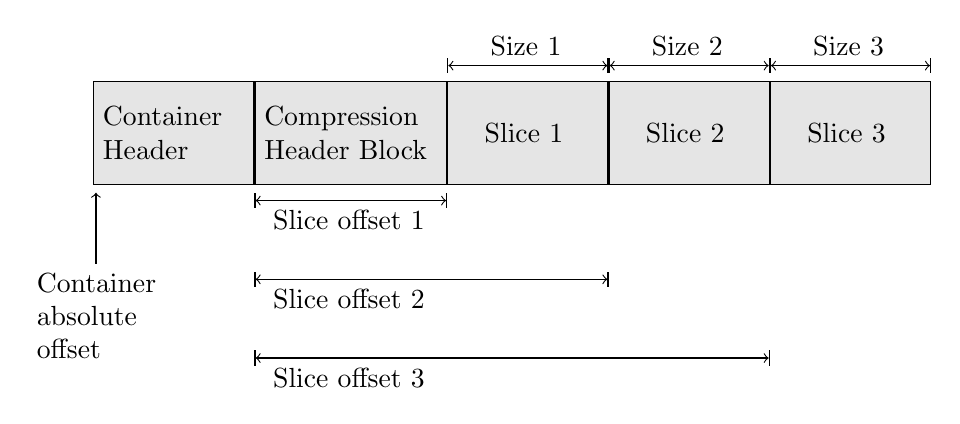
\begin{tikzpicture}[
  boxed/.style={rectangle, draw=black, fill=black!10, minimum height=1.3cm, text width=1.8cm},
]
\node(A) [boxed]{Container Header};
\node(B) [boxed,right,text width=2.2cm] at (A.east){Compression Header Block};
\node(C) [boxed,right] at (B.east){\quad Slice 1};
\node(D) [boxed,right] at (C.east){\quad Slice 2};
\node(E) [boxed,right] at (D.east){\quad Slice 3};

\draw[<-] (A.south west)+(1pt,-0.1cm) -- +(1pt,-1cm)
     node[below, text width=1.5cm]{Container absolute offset};


\draw[|<->|] ([yshift=-0.2cm]B.south west) node[below,xshift=1.2cm]{Slice offset 1}
    -- ([yshift=-0.2cm]B.south east);
\draw[|<->|] ([yshift=-1.2cm]B.south west) node[below,xshift=1.2cm]{Slice offset 2}
    -- ([yshift=-1.2cm]C.south east);
\draw[|<->|] ([yshift=-2.2cm]B.south west) node[below,xshift=1.2cm]{Slice offset 3}
    -- ([yshift=-2.2cm]D.south east);

\draw[|<->|] ([yshift=+0.2cm]C.north west) node[above,xshift=1cm]{Size 1} -- ([yshift=+0.2cm]C.north east);
\draw[|<->|] ([yshift=+0.2cm]D.north west) node[above,xshift=1cm]{Size 2} -- ([yshift=+0.2cm]D.north east);
\draw[|<->|] ([yshift=+0.2cm]E.north west) node[above,xshift=1cm]{Size 3} -- ([yshift=+0.2cm]E.north east);


\end{tikzpicture}
\end{center}

\subsubsection*{BAM index}

BAM indexes are supported by using 4-byte integer pointers called landmarks that 
are stored in container header. BAM index pointer is a 64-bit value with 48 bits 
reserved for the BAM block start position and 16 bits reserved for the in-block 
offset. When used to index CRAM files, the first 48 bits are used to store the 
CRAM container start position and the last 16 bits are used to store the index 
of the landmark in the landmark array stored in  container header. The landmark 
index can be used to access the appropriate slice. 

The above indexing scheme treats CRAM slices as individual records in BAM file. 
This allows to apply BAM indexing to CRAM files, however it introduces some overhead 
in seeking specific alignment start because all preceding records in the slice 
must be read and discarded.

\section{\textbf{Encodings}}
\label{sec:encodings}

% FIXME: we have a mishash of coding, encoding and codec.  We should
% go through the entire document and be consistent.

\subsection{\textbf{Introduction}}

The basic idea for codings is to efficiently represent some values in binary format. 
This can be achieved in a number of ways that most frequently involve some knowledge 
about the nature of the values being encoded, for example, distribution statistics. 
The methods for choosing the best encoding and determining its parameters are very 
diverse and are not part of the CRAM format specification, which only describes 
how the information needed to decode the values should be stored.

Note two of the encodings (Golomb and Golomb-Rice) are listed as deprecated.
These are still formally part of the CRAM specification, but have not been used by the primary implementations and may not be well supported.
Therefore their use is permitted, but not recommended.

\subsubsection*{Offset}

Many of the codings listed below encode positive integer numbers. An integer offset 
value is used to allow any integer numbers and not just positive ones to be encoded. 
It can also be used for monotonically decreasing distributions with the maximum 
not equal to zero. For example, given offset is 10 and the value to be encoded 
is 1, the actually encoded value would be offset+value=11. Then when decoding, 
the offset would be subtracted from the decoded value. 

\subsection{EXTERNAL: codec ID 1}

Can encode types \textit{Byte}, \textit{Integer}.

The EXTERNAL coding is simply storage of data verbatim to an external block with a given ID.
If the type is \textit{Byte} the data is stored as-is, otherwise for \textit{Integer} type the data is stored in ITF8.

\subsubsection*{Parameters}

CRAM format defines the following parameters of EXTERNAL coding: 

\begin{tabular}{|>{\raggedright}p{100pt}|>{\raggedright}p{100pt}|>{\raggedright}p{230pt}|}
\hline
\textbf{Data type} & \textbf{Name} & \textbf{Comment}
\tabularnewline
\hline
itf8 & external id & id of an external block containing the byte stream\tabularnewline
\hline
\end{tabular}

\subsection{Huffman coding: codec ID 3}

Can encode types \textit{Byte}, \textit{Integer}.

Huffman coding replaces symbols (values to encode) by binary codewords, with common symbols having shorter codewords such that the total message of binary codewords is shorter than using uniform binary codeword lengths.
The general process consists of the following steps.

\begin{itemize}
\item Obtain symbol code lengths.
\begin{itemize}
\item If encoding:\\
- Compute symbol frequencies.\\
- Compute code lengths from frequencies.
\item If decoding:\\
- Read code lengths from codec parameters.
\end{itemize}

\item Compute canonical Huffman codewords from code lengths\footnote{\url{https://en.wikipedia.org/wiki/Canonical_Huffman_code}}.

\item Encode or decode bits as per the symbol to codeword table.
Codewords have the ``prefix property'' that no codeword is a prefix of another codeword, enabling unambiguous decode bit by bit.
\end{itemize}

The use of canonical Huffman codes means that we only need to store the code lengths and use the same algorithm in both encoder and decoder to generate the codewords.
This is achieved by ensuring our symbol alphabet has a natural sort order and codewords are assigned in numerical order.

\textbf{Important note: for alphabets with only one value, the codeword will be zero bits long.}
This makes the Huffman codec an efficient mechanism for specifying constant values.

\subsubsection*{Canonical code computation}

\begin{enumerate}
\item Sort the alphabet ascending using bit-lengths and then using numerical order 
of the values.

\item The first symbol in the list gets assigned a codeword which is the same length 
as the symbol's original codeword but all zeros. This will often be a single zero 
('0').

\item Each subsequent symbol is assigned the next binary number in sequence, ensuring
that following codes are always higher in value.

\item When you reach a longer codeword, then after incrementing, append zeros until 
the length of the new codeword is equal to the length of the old codeword.
\end{enumerate}

\subsubsection*{Examples}

\begin{tabular}{|>{\raggedright}p{105pt}|>{\raggedright}p{105pt}|>{\raggedright}p{105pt}|}
\hline
\textbf{Symbol} & \textbf{Code length} & \textbf{Codeword}\tabularnewline
\hline
A & 1 & 0\tabularnewline
\hline
B & 3 & 100\tabularnewline
C & 3 & 101\tabularnewline
D & 3 & 110\tabularnewline
\hline
E & 4 & 1110\tabularnewline
F & 4 & 1111\tabularnewline
\hline
\end{tabular}

\subsubsection*{Parameters}

\begin{tabular}{|>{\raggedright}p{100pt}|>{\raggedright}p{100pt}|>{\raggedright}p{230pt}|}
\hline
\textbf{Data type} & \textbf{Name} & \textbf{Comment}
\tabularnewline
\hline
itf8[ ] & alphabet & list of all encoded symbols (values)\tabularnewline
\hline
itf8[ ] & bit-lengths & array of bit-lengths for each symbol in the alphabet\tabularnewline
\hline
\end{tabular}

\subsection{Byte array coding}

Often there is a need to encode an array of bytes where the length is not predetermined.
For example the read identifiers differ per alignment record, possibly with different lengths, and this length must be stored somewhere.
There are two choices available: storing the length explicitly (BYTE\_ARRAY\_LEN) or continuing to read bytes until a termination value is seen (BYTE\_ARRAY\_STOP).

Note in contrast to this, quality values are known to be the same length as the sequence which is an already known quantity, so this does not need to be encoded using the byte array codecs.

\subsubsection*{BYTE\_ARRAY\_LEN: codec ID 4}

Can encode types \textit{Byte[ ]}.

Byte arrays are captured length-first, meaning that the length of every array element is written using an additional encoding.
For example this could be a HUFFMAN encoding or another EXTERNAL block.
The length is decoded first followed by the data, followed by the next length and data, and so on.

This encoding can therefore be considered as a nested encoding, with each pair of nested encodings containing their own set of parameters.
The byte stream for parameters of the BYTE\_ARRAY\_LEN encoding is therefore the concatenation of the length and value encoding parameters as described in section~\ref{subsec:writing-bytes}.

The parameter for BYTE\_ARRAY\_LEN are listed below:

\begin{tabular}{|>{\raggedright}p{100pt}|>{\raggedright}p{100pt}|>{\raggedright}p{230pt}|}
\hline
\textbf{Data type} & \textbf{Name} & \textbf{Comment}
\tabularnewline
\hline
encoding\texttt{<}int\texttt{>} & lengths encoding & an encoding describing how 
the arrays lengths are captured\tabularnewline
\hline
encoding\texttt{<}byte\texttt{>} & values encoding & an encoding describing how 
the values are captured\tabularnewline
\hline
\end{tabular}

For example, the bytes specifying a BYTE\_ARRAY\_LEN encoding, including the codec and parameters, for a 16-bit X0 auxiliary tag (``X0C'') may use HUFFMAN encoding to specify the length (always 2 bytes) and an EXTERNAL encoding to store the value to an external block with ID 200.

\begin{tabular}{lll}
\hline
\textbf{Bytes} & & \textbf{Meaning}\\
\hline
\texttt{0x04}         & & BYTE\_ARRAY\_LEN codec ID                                    \\
\texttt{0x0a}         & & 10 remaining bytes of BYTE\_ARRAY\_LEN parameters            \\
\\
\texttt{0x03}         & & HUFFMAN codec ID, for aux tag lengths                        \\
\texttt{0x04}         & & 4 more bytes of HUFFMAN parameters                           \\
\texttt{0x01}         & & Alphabet array size = 1                                      \\
\texttt{0x02}         & & alphabet symbol; (length = 2)                                \\
\texttt{0x01}         & & Codeword array size = 1                                      \\
\texttt{0x00}         & & Code length = 0 (zero bits needed as alphabet is size 1)     \\
\\
\texttt{0x01}         & & EXTERNAL codec ID, for aux tag values                        \\
\texttt{0x02}         & & 2 more bytes of EXTERNAL parameters                          \\
\texttt{0x80 0xc8}    & & ITF8 encoding for block ID 200                               \\
\hline
\end{tabular}



\subsubsection*{BYTE\_ARRAY\_STOP: codec ID 5}

Can encode types \textit{Byte[ ]}.

Byte arrays are captured as a sequence of bytes terminated by a special stop byte.
The data returned does not include the stop byte itself.
In contrast to BYTE\_ARRAY\_LEN the value is always encoded with EXTERNAL so the parameter is an external id instead of another encoding.

\begin{tabular}{|>{\raggedright}p{100pt}|>{\raggedright}p{100pt}|>{\raggedright}p{230pt}|}
\hline
\textbf{Data type} & \textbf{Name} & \textbf{Comment}
\tabularnewline
\hline
byte & stop byte & a special byte treated as a delimiter\tabularnewline
\hline
itf8 & external id & id of an external block containing the byte stream\tabularnewline
\hline
\end{tabular}

\subsection{Beta coding: codec ID 6}

Can encode types \textit{Integer}.

\subsubsection*{Definition}

Beta coding is a most common way to represent numbers in \emph{binary notation} and is sometimes referred to as binary coding.
The decoder reads the specified fixed number of bits (most significant first) and subtracts the offset value to get the decoded integer.

\subsubsection*{Parameters}

CRAM format defines the following parameters of beta coding: 

\begin{tabular}{|>{\raggedright}p{144pt}|>{\raggedright}p{144pt}|>{\raggedright}p{144pt}|}
\hline
\textbf{Data type} & \textbf{Name} & \textbf{Comment}\tabularnewline
\hline
itf8 & offset & offset is subtracted from each value during decode\tabularnewline
\hline
itf8 & length & the number of bits used\tabularnewline
\hline
\end{tabular}

\subsubsection*{Examples}

If we have integer values in the range 10 to 15 inclusive, the largest value would traditionally need 4 bits, but with an offset of -10 we can hold values 0 to 5, using a fixed size of 3 bits.
Using fixed Offset and Length coming from the beta parameters, we decode these values as:

\begin{tabular}{|>{\raggedright}p{105pt}|>{\raggedright}p{105pt}|>{\raggedright}p{105pt}|>{\raggedright}p{105pt}|}
\hline
Offset & Length & \textbf{Bits} & \textbf{Value}\tabularnewline
\hline
-10 & 3 & 000 & 10\tabularnewline
\hline
-10 & 3 & 001 & 11\tabularnewline
\hline
-10 & 3 & 010 & 12\tabularnewline
\hline
-10 & 3 & 011 & 13\tabularnewline
\hline
-10 & 3 & 100 & 14\tabularnewline
\hline
-10 & 3 & 101 & 15\tabularnewline
\hline
\end{tabular}

\subsection{Subexponential coding: codec ID 7}

Can encode types \textit{Integer}.

\subsubsection*{Definition}

Subexponential coding\footnote{Fast progressive lossless image compression, Paul G. Howard and Jeffrey Scott Vitter, 1994. \url{http://www.ittc.ku.edu/~jsv/Papers/HoV94.progressive_FELICS.pdf}} is parametrized by a non-negative integer $k$.
For values $n < 2^{k+1}$ subexponential coding produces codewords identical to Rice coding \footnote{\url{https://en.wikipedia.org/wiki/Golomb_coding\#Rice_coding}}.  For larger values it grows logarithmically with $n$.

\subsubsection*{Encoding}

\begin{enumerate}
\item Add $\mathit{offset}$ to $n$.

\item Determine $u$ and $b$ values from $n$
\begin{align*}
b =
\begin{cases}
  \ k                        & \text{ if $n < 2^k$} \\
  \ \lfloor log_{2}n \rfloor & \text{ if $n \ge 2^k$}
\end{cases}
&\
&u =
\begin{cases}
  \ 0     & \text{ if $n < 2^k$} \\
  \ b-k+1 & \text{ if $n \ge 2^k$}
\end{cases}
\end{align*}

\item Write $u$ in unary form; $u$ 1 bits followed by a single 0 bit.

\item Write the bottom $b$-bits of $n$ in binary form.
\end{enumerate}

\subsubsection*{Decoding}

\begin{enumerate}
\item Read $u$ in unary form, counting the number of leading 1s (prefix) in the codeword (discard the trailing 0 bit).

\item Determine $n$ via:
\begin{enumerate}
\item if $u = 0$ then read $n$ as a $k$-bit binary number.
\item if $u \ge 1$ then read $x$ as a $(u + k - 1)$-bit binary. Let $n = 2^{u+k-1} + x$.
\end{enumerate}

\item Subtract $\mathit{offset}$ from $n$.
\end{enumerate}

\subsubsection*{Examples}

\begin{tabular}{|>{\raggedright}p{105pt}|>{\raggedright}p{105pt}|>{\raggedright}p{105pt}|>{\raggedright}p{105pt}|}
\hline
\textbf{Number} & \textbf{Codeword, k=0} & \textbf{Codeword, k=1} & \textbf{Codeword, 
k=2}\tabularnewline
\hline
0 & 0 & 00 & 000\tabularnewline
\hline
1 & 10 & 01 & 001\tabularnewline
\hline
2 & 1100 & 100 & 010\tabularnewline
\hline
3 & 1101 & 101 & 011\tabularnewline
\hline
4 & 111000 & 11000 & 1000\tabularnewline
\hline
5 & 111001 & 11001 & 1001\tabularnewline
\hline
6 & 111010 & 11010 & 1010\tabularnewline
\hline
7 & 111011 & 11011 & 1011\tabularnewline
\hline
8 & 11110000 & 1110000 & 110000\tabularnewline
\hline
9 & 11110001 & 1110001 & 110001\tabularnewline
\hline
10 & 11110010 & 1110010 & 110010\tabularnewline
\hline
\end{tabular}

\subsubsection*{Parameters}

\begin{tabular}{|>{\raggedright}p{100pt}|>{\raggedright}p{100pt}|>{\raggedright}p{230pt}|}
\hline
\textbf{Data type} & \textbf{Name} & \textbf{Comment}
\tabularnewline
\hline
itf8 & offset & offset is subtracted from each value during decode\tabularnewline
\hline
itf8 & k & the order of the subexponential coding\tabularnewline
\hline
\end{tabular}

\subsection{Gamma coding: codec ID 9}

Can encode types \textit{Integer}.

\subsubsection*{Definition}

\emph{Elias gamma code} is a prefix encoding of positive integers. This is a combination 
of unary coding and beta coding. The first is used to capture the number of bits 
required for beta coding to capture the value. 

\subsubsection*{Encoding}

\begin{enumerate}
\item Write it in binary.

\item Subtract $1$ from the number of bits written in step 1 and prepend that many zeros.

\item An equivalent way to express the same process:

\item Separate the integer into the highest power of $2$ it contains ($2N$) and the remaining 
$N$ binary digits of the integer.

\item Encode $N$ in unary; that is, as $N$ zeroes followed by a one.

\item Append the remaining $N$ binary digits to this representation of $N$.
\end{enumerate}

\subsubsection*{Decoding}

\begin{enumerate}
\item Read and count 0s from the stream until you reach the first 1. Call this count 
of zeroes $N$.

\item Considering the one that was reached to be the first digit of the integer, with 
a value of $2N$, read the remaining $N$ digits of the integer.
\end{enumerate}

\subsubsection*{Examples}

\begin{tabular}{|>{\raggedright}p{76pt}|>{\raggedright}p{107pt}|}
\hline
\textbf{Value} & \textbf{Codeword}\tabularnewline
\hline
1 & 1\tabularnewline
\hline
2 & 010\tabularnewline
\hline
3 & 011\tabularnewline
\hline
4 & 00100\tabularnewline
\hline
\end{tabular}

\subsubsection*{Parameters}

\begin{tabular}{|>{\raggedright}p{144pt}|>{\raggedright}p{144pt}|>{\raggedright}p{144pt}|}
\hline
\textbf{Data type} & \textbf{Name} & \textbf{Comment}\tabularnewline
\hline
itf8 & offset & offset to subtract from each value after decode\tabularnewline
\hline
\end{tabular}

\subsection{DEPRECATED: Golomb coding: codec ID 2}

Can encode types \textit{Integer}.

Note this codec has not been used in any known CRAM implementation since before CRAM v1.0.
Nor is it implemented in some of the major software.
Therefore its use is not recommended.

\subsubsection*{Definition}

\emph{Golomb encoding} is a prefix encoding optimal for representation of random 
positive numbers following geometric distribution. 

\subsubsection*{Encoding}

\begin{enumerate}
\item Fix the parameter $M$ to an integer value.

\item For $N$, the number to be encoded, find

\begin{enumerate}
\item quotient $q = \lfloor N/M \rfloor$

\item remainder $r = N \bmod M$
\end{enumerate}

\item Generate Codeword

\begin{enumerate}
\item The Code format : \texttt{<}Quotient Code\texttt{>}\texttt{<}Remainder Code\texttt{>}, 
where

\item Quotient Code (in unary coding)

\begin{enumerate}
\item Write a $q$-length string of 1 bits

\item Write a 0 bit
\end{enumerate}

\item Remainder Code (in truncated binary encoding)

Set $b=\lceil log_{2}(M) \rceil$

\begin{enumerate}
\item If $r < 2^{b}-M$ code $r$ as plain binary using $b-1$ bits.

\item If $r \ge 2^{b}-M$ code the number $r+2^{b}-M$ in plain binary representation 
using $b$ bits.
\end{enumerate}
\end{enumerate}
\end{enumerate}

\subsubsection*{Decoding}

\begin{enumerate}
\item Read $q$ via unary coding: count the number of 1 bits and consume the following 0 bits.
\item Set $b=\lceil log_{2}(M) \rceil$
\item Read $r$ via $b-1$ bits of binary coding
\item If $r \ge 2^{b}-M$
\begin{enumerate}
\item Read 1 single bit, $x$.
\item Set $r = r*2 + x - (2^{b}-M)$
\end{enumerate}
\item Value is $q*M + r - \mathit{offset}$
\end{enumerate}

\subsubsection*{Examples}

\begin{tabular}{|>{\raggedright}p{76pt}|>{\raggedright}p{107pt}|}
\hline
\textbf{Number} & \textbf{Codeword, M=10, (thus b=4)}\tabularnewline
\hline
0 & 0000\tabularnewline
\hline
4 & 0100\tabularnewline
\hline
10 & 10000\tabularnewline
\hline
26 & 1101100\tabularnewline
\hline
42 & 11110010\tabularnewline
\hline
\end{tabular}

\subsubsection*{Parameters}

Golomb coding takes the following parameters: 

\begin{tabular}{|>{\raggedright}p{144pt}|>{\raggedright}p{144pt}|>{\raggedright}p{144pt}|}
\hline
\textbf{Data type} & \textbf{Name} & \textbf{Comment}\tabularnewline
\hline
itf8 & offset & offset is added to each value\tabularnewline
\hline
itf8 & M & the golomb parameter (number of bins)\tabularnewline
\hline
\end{tabular}

\subsection{DEPRECATED: Golomb-Rice coding: codec ID 8}

Can encode types \textit{Integer}.

Note this codec has not been used in any known CRAM implementation since before CRAM v1.0.
Nor is it implemented in some of the major software.
Therefore its use is not recommended.

Golomb-Rice coding is a special case of Golomb coding when the M parameter is a power of 2.
The reason for this coding is that the division operations in Golomb coding can be replaced with bit shift operators as well as avoiding the extra $r < 2^{b}-M$ check.

\section{\textbf{External compression methods}}

External encoding operates on bytes only. Therefore any data series must be translated into bytes before sending data into an external block.
The following methods are defined.
Exact definitions of these methods are in their respective internet links or the ancillary \textit{CRAMcodecs} document found along side this specification.

Integer values are written as ITF8, which then can be translated into an array 
of bytes. 

Strings, like read name, are translated into bytes according to UTF8 rules. In 
most cases these should coincide with ASCII, making the translation trivial.

Each method has an associated numeric code which is defined in Section~\ref{sec:block-struct}.

\subsection{\textbf{Gzip}}

The Gzip specification is defined in RFC 1952.
Gzip in turn is an encapsulation on the Deflate algorithm defined in RFC 1951.

\subsection{\textbf{Bzip2}}

First available in CRAM v2.0.

Bzip2 is a compression method utilising the Burrows Wheeler Transform, Move To Front transform, Run Length Encoding and a Huffman entropy encoder. 
It is often superior to Gzip for textual data.

An informal format specification exists:\\
\url{https://github.com/dsnet/compress/blob/master/doc/bzip2-format.pdf}

\subsection{\textbf{LZMA}}

First available in CRAM v3.0.

LZMA is the Lempel-Ziv Markov chain algorithm.
CRAM uses the xz Stream format to encapsulate this algorithm, as defined in \url{https://tukaani.org/xz/xz-file-format.txt}.

\subsection{\textbf{rANS4x8 codec}}

First available in CRAM v3.0.

rANS is the range-coder variant of the Asymmetric Numerical
System\footnote{J. Duda, \textit{Asymmetric numeral systems: entropy
    coding combining speed of Huffman coding with compression rate of
    arithmetic coding}, \url{http://arxiv.org/abs/1311.2540}}.

``4x8'' refers to 4-way interleaving with 8-bit renormalisation.\newline
This variant of rANS first appeared in CRAM v3.0.

Details of this algorithm have been moved to the \textit{CRAMcodecs} document.

\subsection{\textbf{rANS4x16 codec}}

First available in CRAM v3.1.

``4x16'' refers to 4-way interleaving with 16-bit renormalisation.\newline
This variant of rANS first appeared in CRAM v3.1.

Details of this algorithm are listed in the \textit{CRAMcodecs} document.

\subsection{\textbf{adaptive arithemtic coding}}

First available in CRAM v3.1.

An entropy encoder that is slower but slightly more concise than
rANS.  It achieves this by adapting the probabilities as it compresses
and decompresses instead of using a fixed table.

Details of this algorithm are listed in the \textit{CRAMcodecs} document.

\subsection{\textbf{fqzcomp codec}}

First available in CRAM v3.1.

This is a method dedicated to compression of quality values.

Details of this algorithm are listed in the \textit{CRAMcodecs} document.

\subsection{\textbf{name tokeniser}}

First available in CRAM v3.1.

This is a method dedicated to compression of read names.

Details of this algorithm are listed in the \textit{CRAMcodecs} document.

\section{\textbf{Appendix}}
\subsection{\textbf{Choosing the container size}}

CRAM format does not constrain the size of the containers. However, the following 
should be considered when deciding the container size:

$\bullet$ Data can be compressed better by using larger containers

$\bullet$ Random access performance is better for smaller containers 

$\bullet$ Streaming is more convenient for small containers

$\bullet$ Applications typically buffer containers into memory

We recommend 1 megabyte containers. They are small enough to provide good random access
and streaming performance while being large enough to provide good compression. 
1\MB\ containers are also small enough to fit into the L2 cache of most modern CPUs.

Some simplified examples are provided below to fit data into 1\MB\ containers.

\textbf{Unmapped short reads with bases, read names, recalibrated and original 
quality scores}

We have 10,000 unmapped short reads (100bp) with read names, recalibrated and original 
quality scores. We estimate 0.4 bits/base (read names) + 0.4 bits/base (bases) 
+ 3 bits/base (recalibrated quality scores) + 3 bits/base (original quality scores) 
$\approx$ 7 bits/base. Space estimate is $10\,000 \times 100 \times 7 \bits
\approx 0.9 \MB$. Data could be stored in a single container.

\textbf{Unmapped long reads with bases, read names and quality scores}

We have 10,000 unmapped long reads (10kb) with read names and quality scores. We 
estimate: 0.4 bits/base (bases) + 3 bits/base (original quality scores) $\approx$
3.5 bits/base. Space estimate is $10\,000 \times 10\,000 \times 3.5 \bits
\approx 42 \MB$. Data could be stored in $42 \times 1\MB$ containers.

\textbf{Mapped short reads with bases, pairing and mapping information}

We have 250,000 mapped short reads (100bp) with bases, pairing and mapping information. 
We estimate the compression to be 0.2 bits/base. Space estimate is $250\,000 \times 100
\times 0.2 \bits \approx 0.6 \MB$. Data could be stored in a single
container.

\textbf{Embedded reference sequences}

We have a reference sequence (10Mb). We estimate the compression to be 2 bits/base. 
Space estimate is $10\,000\,000 \times 2 \bits \approx 2.4 \MB$. Data
could be written into three containers: $1\MB + 1\MB + 0.4\MB$.

\newpage

\subsection{CRAM History}

\subsubsection*{Pre-CRAM: 2010}

The primary concepts and ideas of CRAM stem from work at the European
Bioinformatics Institute in 2010 and 2011, published in:

\begin{quote}\small
Markus Hsi-Yang Fritz,
Rasko Leinonen, Guy Cochrane, and Ewan Birney,
\textbf{Efficient storage of high throughput DNA sequencing data using reference-based compression},
{\sl Genome Res.}~2011~21: 734--740;
\href{http://dx.doi.org/doi:10.1101/gr.114819.110}{doi:10.1101/gr.114819.110};
{\sc pmid:}21245279.
\end{quote}

\subsubsection*{CRAM 0.x: 2011}

Vadim Zalunin implemented the ideas in the paper, now named CRAM, in
the Java CRAMtools package.  This included versions from 0.3 to 0.86\footnote{\url{https://github.com/vadimzalunin/crammer/releases}}.

\subsubsection*{CRAM 1.0: 2012}

The first official launch of the CRAM specification, in the Java
CRAMtools package\footnote{\url{https://github.com/enasequence/cramtools}}

This was publicised at \url{https://github.com/enasequence/cramtools}.

\subsubsection*{CRAM 2.0: 2013}

Reimplementing CRAM in C
\footnote{Staden IO\_Lib 1.13.0 and later HTSlib 0.2.0} exposed a number of issues with the
1.0 specification and disparities between the specification text and
the Java implementation.  CRAM 2.0 unified implementation with
specification.

Other changes included:

\begin{itemize}
\item Support for multiple references per container, to permit storage
of highly fragmented assemblies.

\item Soft-clips and inserted bases moved to their own separate
data-series instead of sharing one.

\item Slice headers contain meta-data tracking the number of records
and bases.

\item Corrected the BF (bam flag) data series to match the BAM
specification.

\item Improved encoding of auxiliary tags.
\end{itemize}

\subsubsection*{CRAM 2.1: 2014}

This is the first version to appear in HTSJDK (version 1.127), ported
from the Java CRAMtools package.

\begin{itemize}
\item EOF blocks are added in order to spot truncated files.
\end{itemize}

\subsubsection*{CRAM 3.0: 2014}

Primarily this is an optimisation of size and speed.

\begin{itemize}
\item Inclusion of LZMA compression library.
\item Inclusion of the custom rANS Order-0 and Order-1 entropy encoders.
\item Checksums added to all file format structures to ensure data integrity.
\end{itemize}

\subsubsection*{CRAM 3.1: 2023}

Note: the formal draft appeared in 2019, and was initially
demonstrated in 2016.

This adds new EXTERNAL compression methods, described in the separate
CRAMcodecs document, and expands the list of permitted ``methods'' in
the CRAM Block structure.

The aim of the new compression methods is improved compression, both
performance with the newer SIMD rANS implementation and file size with
custom name tokeniser and quality codec.

The format is otherwise identical to 3.0.

\newpage

\subsection{\textbf{Contributors and Acknowledgements}}

\begin{itemize}
\item
Markus Fritz, Rasko Leinonen, Guy Cochrane and Ewan Birney (EBI):
Initial ideas behind CRAM.

\item Vadim Zalunin (EBI):
Initial JAVA implementation of CRAM and previous maintainer of CRAM specification.

\item James Bonfield (Sanger Institute):
Initial C implementation of CRAM and current maintainer of CRAM
specification.

\item Joel Thibault (Broad Institute):
previous maintainer of CRAM specification.

\item Chris Norman (Broad Institute):
previous maintainer of CRAM specification and worked on
the HTSJDK implementation.

\item Robert Buels (UC Berkeley): First JavaScript implementation of CRAM

\item Michael Macias (St Jude Children's Research Hospital): First Rust implementation of CRAM

\item Other specification contributors include: John Marshall, Rishi Nag,
Kenta Sato, Artem Tarasov and Jason Travis.

\item Plus a big thank you to everyone who has raised GitHub issues
and/or helped us improve the specification in other ways.
\end{itemize}

\end{document}

\title{CRAM format specification (version 3.1)}
\author{samtools-devel@lists.sourceforge.net}
\date{\headdate}
\maketitle


\begin{quote}\small
The master version of this document can be found at
\url{https://github.com/samtools/hts-specs}.\\
This printing is version~\commitdesc\ from that repository,
last modified on the date shown above.
\end{quote}

\begin{center}
\textit{license: Apache 2.0}
\end{center}
\vspace*{1em}

\section{\textbf{Overview}}

This specification describes the CRAM 3.0 and 3.1 formats.

CRAM has the following major objectives:

\begin{enumerate}
\item Significantly better lossless compression than BAM

\item Full compatibility with BAM

\item Effortless transition to CRAM from using BAM files

\item Support for controlled loss of BAM data
\end{enumerate}

The first three objectives allow users to take immediate advantage of the CRAM 
format while offering a smooth transition path from using BAM files. The fourth 
objective supports the exploration of different lossy compression strategies and 
provides a framework in which to effect these choices. Please note that the CRAM 
format does not impose any rules about what data should or should not be preserved. 
Instead, CRAM supports a wide range of lossless and lossy data preservation strategies 
enabling users to choose which data should be preserved.

Data in CRAM is stored either as CRAM records or using one of the general purpose 
compressors (gzip, bzip2). CRAM records are compressed using a number of different 
encoding strategies. For example, bases are reference compressed by encoding base
differences rather than storing the bases themselves.\footnote{Markus Hsi-Yang Fritz,
Rasko Leinonen, Guy Cochrane, and Ewan Birney,
\textbf{Efficient storage of high throughput DNA sequencing data using reference-based compression},
{\sl Genome Res.}~2011~21: 734--740;
\href{http://dx.doi.org/doi:10.1101/gr.114819.110}{doi:10.1101/gr.114819.110};
{\sc pmid:}21245279.}

\section{\textbf{Data types}}

CRAM specification uses logical data types and storage data types; logical data 
types are written as words (e.g. int) while physical data types are written using 
single letters (e.g. i). The difference between the two is that storage data types 
define how logical data types are stored in CRAM. Data in CRAM is stored either 
as bits or bytes. Writing values as bits and bytes is described in detail 
below.

\subsection{\textbf{Logical data types}}

\begin{description}
\item[Byte]\ \newline
Signed byte (8 bits).

\item[Integer]\ \newline
Signed 32-bit integer. 

\item[Long]\ \newline
Signed 64-bit integer. 

\item[Array]\ \newline
An array of any logical data type: array\texttt{<}type\texttt{>}
\end{description}

% \begin{tabular}{ll}
% \textbf{Byte}    & Signed byte (8 bits).  \\
% \\
% \textbf{Integer} & Signed 32-bit integer. \\
% \\
% \textbf{Long}    & Signed 64-bit integer. \\
% \\
% \textbf{Array}   & An array of any logical data type: \texttt{<}type\texttt{>}[ ] \\
% \end{tabular}

\subsection{\textbf{Writing bits to a bit stream}}

A bit stream consists of a sequence of 1s and 0s. The bits are written most significant 
bit first where new bits are stacked to the right and full bytes on the left are 
written out. In a bit stream the last byte will be incomplete if less than 8 bits 
have been written to it. In this case the bits in the last byte are shifted to 
the left.

\subsubsection*{Example of writing to bit stream}

Let's consider the following example. The table below shows a sequence of write 
operations: 

\begin{tabular}{|l|l|l|l|l|}
\hline
\textbf{Operation order} & \textbf{Buffer state before} & \textbf{Written bits} & \textbf{Buffer state after} & \textbf{Issued bytes}\tabularnewline
\hline
1 & 0x0 & 1 & 0x1 & -\tabularnewline
\hline
2 & 0x1 & 0 & 0x2 & -\tabularnewline
\hline
3 & 0x2 & 11 & 0xB & -\tabularnewline
\hline
4 & 0xB & 0000 0111 & 0x7 & 0xB0\tabularnewline
\hline
\end{tabular}

After flushing the above bit stream the following bytes are written: 0xB0 0x70. 
Please note that the last byte was 0x7 before shifting to the left and became 0x70 
after that:

\texttt{> echo "obase=16; ibase=2; 00000111" \textbar{} bc\\
7\\
\\
> echo "obase=16; ibase=2; 01110000" \textbar{} bc\\
70}

And the whole bit sequence: 

\texttt{> echo "obase=2; ibase=16; B070" \textbar{} bc\\
1011000001110000}

When reading the bits from the bit sequence it must be known that only 12 bits 
are meaningful and the bit stream should not be read after that. 

\subsubsection*{Note on writing to bit stream}

When writing to a bit stream both the value and the number of bits in the value 
must be known. This is because programming languages normally operate with bytes 
(8 bits) and to specify which bits are to be written requires a bit-holder, for 
example an integer, and the number of bits in it. Equally, when reading a value 
from a bit stream the number of bits must be known in advance. In case of prefix 
codes (e.g. Huffman) all possible bit combinations are either known in advance 
or it is possible to calculate how many bits will follow based on the first few 
bits. Alternatively, two codes can be combined, where the first contains the number 
of bits to read. 

\subsection{\textbf{Writing bytes to a byte stream}}
\label{subsec:writing-bytes}

The interpretation of byte stream is straightforward. CRAM uses \emph{little endianness}
for bytes when applicable and defines the following storage data types:

\begin{description}

\item[Boolean (bool)]\ \newline
Boolean is written as 1-byte with 0x0 being `false' and 0x1 being `true'.

\item[Integer (int32)]\ \newline
Signed 32-bit integer, written as 4 bytes in little-endian byte order.

\item[Long (int64)]\ \newline
Signed 64-bit integer, written as 8 bytes in little-endian byte order.

\item[ITF-8 integer (itf8)]\ \newline
This is an alternative way to write an integer value. The idea is similar to UTF-8 
encoding and therefore this encoding is called ITF-8 (Integer Transformation Format 
- 8 bit). 

The most significant bits of the first byte have special meaning and are called 
`prefix'. These are 0 to 4 true bits followed by a 0. The number of 1's denote 
the number of bytes to follow. To accommodate 32 bits such representation requires 
5 bytes with only 4 lower bits used in the last byte 5.

\item[LTF-8 long (ltf8)]\ \newline
See ITF-8 for more details. The only difference between ITF-8 and LTF-8 is the 
number of bytes used to encode a single value. To do so 64 bits are required and 
this can be done with 9 byte at most with the first byte consisting of just 1s 
or 0xFF value. 

\item[{Array (array\texttt{<}type\texttt{>})}]\ \newline
A variable sized array with an explicitly written dimension.
Array length is written first as integer (itf8), followed by the elements of the array.

Implicit or fixed-size arrays are also used, written as \textit{type}\texttt{[ ]} or \textit{type}\texttt{[4]} (for example).
These have no explicit dimension included in the file format and instead rely on the specification itself to document the array size.


\item[{Encoding}]\ \newline
Encoding is a data type that specifies how data series have been compressed. Encodings 
are defined as encoding\texttt{<}type\texttt{>} where the type is a logical data 
type as opposed to a storage data type.

An encoding is written as follows. The first integer (itf8) denotes the codec id 
and the second integer (itf8) the number of bytes in the following encoding-specific 
values. 

Subexponential encoding example: 

\begin{tabular}{|l|l|l|}
\hline
\textbf{Value} & \textbf{Type} & \textbf{Name}\tabularnewline
\hline
0x7 & itf8 & codec id\tabularnewline
\hline
0x2 & itf8 & number of bytes to follow\tabularnewline
\hline
0x0 & itf8 & offset\tabularnewline
\hline
0x1 & itf8 & K parameter\tabularnewline
\hline
\end{tabular}

The first byte ``0x7'' is the codec id. 

The next byte ``0x2'' denotes the length of the bytes to follow (2). 

The subexponential encoding has 2 parameters: integer (itf8) offset and integer (itf8) K.

offset = 0x0 = 0

K = 0x1 = 1


\item[{Map}]\ \newline
A map is a collection of keys and associated values. A map with N keys is written 
as follows: 

\begin{tabular}{|l|l|l|l|l|l|l|l|}
\hline
size in bytes & N & key 1 & value 1 & key ... & value ... & key N & value N\tabularnewline
\hline
\end{tabular}

Both the size in bytes and the number of keys are written as integer (itf8). Keys 
and values are written according to their data types and are specific to each map.

\item[String]\ \newline
A string is represented as byte arrays using UTF-8 format. Read names, reference 
sequence names and tag values with type `Z' are stored as UTF-8.

\end{description}


\section{\textbf{Encodings }}

Encoding is a data structure that captures information about compression details 
of a data series that are required to uncompress it. This could be a set of constants 
required to initialize a specific decompression algorithm or statistical properties 
of a data series or, in case of data series being stored in an external block, 
the block content id. 

Encoding notation is defined as the keyword `encoding' followed by its data type 
in angular brackets, for example `encoding\texttt{<}byte\texttt{>}' stands for 
an encoding that operates on a data series of data type `byte'. 

Encodings may have parameters of different data types, for example the EXTERNAL 
encoding has only one parameter, integer id of the external block. The following 
encodings are defined: 

\begin{tabular}{|l|l|>{\raggedright}p{155pt}|>{\raggedright}p{160pt}|}
\hline
\textbf{Codec} & \textbf{ID} & \textbf{Parameters} & \textbf{Comment}\tabularnewline
\hline
NULL & 0 & none & series not preserved\tabularnewline
\hline
EXTERNAL & 1 & int block content id & the block content identifier used to associate 
external data blocks with data series\tabularnewline
\hline
Deprecated (GOLOMB) & 2 & int offset, int M & Golomb coding\tabularnewline
\hline
HUFFMAN & 3 & array\texttt{<}int\texttt{>}, array\texttt{<}int\texttt{>} & coding with int/byte values\tabularnewline
\hline
BYTE\_ARRAY\_LEN & 4 & encoding\texttt{<}int\texttt{>} array length, encoding\texttt{<}byte\texttt{>} 
bytes & coding of byte arrays with array length\tabularnewline
\hline
BYTE\_ARRAY\_STOP & 5 & byte stop, int external block\linebreak{}
content id & coding of byte arrays with a stop value \tabularnewline
\hline
BETA & 6 & int offset, int number of bits & binary coding\tabularnewline
\hline
SUBEXP & 7 & int offset, int K & subexponential coding\tabularnewline
\hline
Deprecated (GOLOMB\_RICE) & 8 & int offset, int log$_{\text{2}}$m & Golomb-Rice coding\tabularnewline
\hline
GAMMA & 9 & int offset & Elias gamma coding\tabularnewline
\hline
\end{tabular}

See section~\ref{sec:encodings} for more detailed descriptions of all the above coding algorithms and their parameters.

\section{\textbf{Checksums}}
The checksumming is used to ensure data integrity. The following checksumming algorithms are used in CRAM.
\subsection{\textbf{CRC32}}
This is a cyclic redundancy checksum 32-bit long with the polynomial 0x04C11DB7. Please refer to \href{http://www.itu.int/rec/recommendation.asp?type=folders&lang=e&parent=T-REC-V.42}{ITU-T V.42} for more details. The value of the CRC32 hash function is written as an integer.
\subsection{\textbf{CRC32 sum}}
CRC32 sum is a combination of CRC32 values by summing up all individual CRC32 values modulo 2\textsuperscript{32}. 

\section{\textbf{File structure}}

The overall CRAM file structure is described in this section. Please refer to other 
sections of this document for more detailed information. 

A CRAM file consists of a fixed length file definition, followed by a CRAM header container,
then zero or more data containers, and finally a special end-of-file container.

\begin{center}
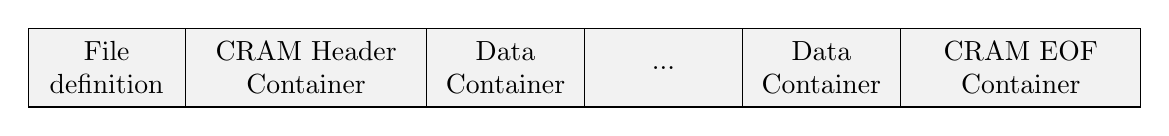
\begin{tikzpicture}[
  every node/.style={scale=1.0},
  boxes/.style={rectangle split,rectangle split parts=#1,draw,rectangle split horizontal,text width=5em,align=center,minimum height=1cm,fill=black!5,on grid},
  notes/.style={text width=20em,align=center,minimum height=1cm,on grid},
]
\node (file) [boxes=6] {
\nodepart{one}File definition
\nodepart[text width=8em]{two}CRAM Header Container
\nodepart{three}Data Container
\nodepart{four}...
\nodepart{five}Data Container
\nodepart[text width=8em]{six}CRAM EOF Container
};
\end{tikzpicture}

Figure 1: A CRAM file consists of a file definition, followed by a header container, then other containers.
\end{center}

Containers consist of one or more blocks. The first container, called the CRAM header container,
is used to store a textual header as described in the SAM specification (see the section 7.1).

\begin{center}
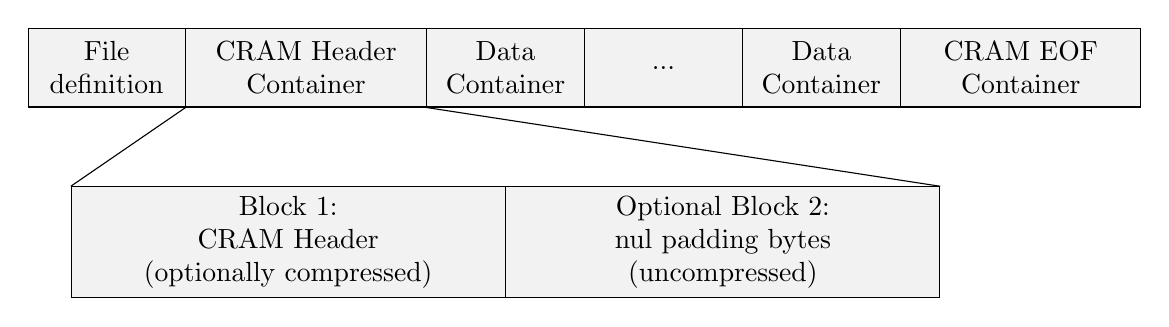
\begin{tikzpicture}[
  every node/.style={scale=1.0},
  boxes/.style={rectangle split,rectangle split parts=#1,draw,rectangle split horizontal,text width=5em,align=center,minimum height=1cm,fill=black!5,on grid},
  notes/.style={text width=20em,align=center,minimum height=1cm,on grid},
]
\node (file) [boxes=6] {
\nodepart{one}File definition
\nodepart[text width=8em]{two}CRAM Header Container
\nodepart{three}Data Container
\nodepart{four}...
\nodepart{five}Data Container
\nodepart[text width=8em]{six}CRAM EOF Container
};

\node (header) [boxes=2,below=1 of file.three south, text width=15em] {
\nodepart{one}Block 1:\break
CRAM Header\break
(optionally compressed)
\nodepart{two}Optional Block 2:\break
nul padding bytes\break
(uncompressed)
};
\draw (file.one split south) to (header.north west);
\draw (file.two split south) to (header.north east);
\end{tikzpicture}

Figure 2: The the first container holds the CRAM header text.
\end{center}

Each container starts with a container header structure followed by
one or more blocks.
The first block in each container is the compression header block
giving details of how to decode data in subsequent blocks.
Each block starts with a block header structure followed by the block
data.

\begin{center}
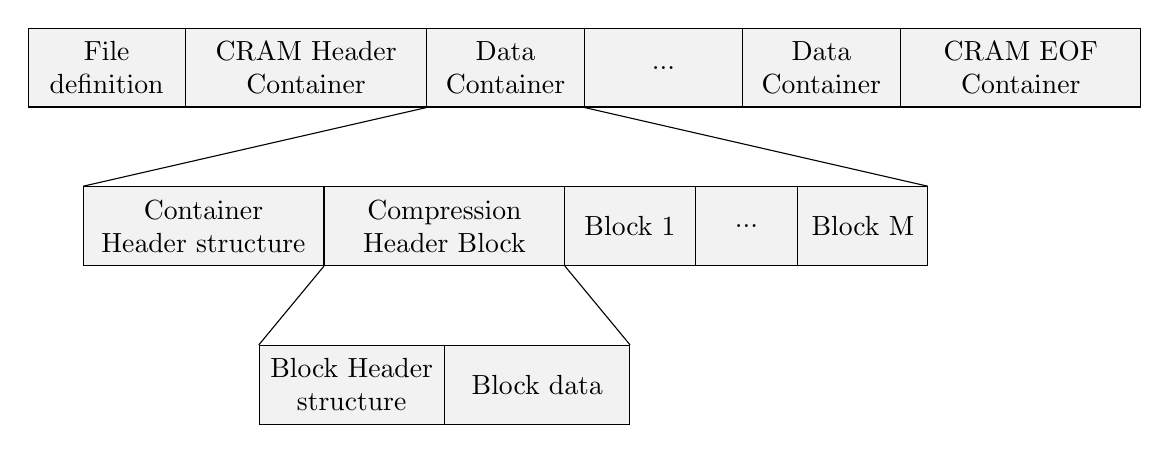
\begin{tikzpicture}[
  every node/.style={scale=1.0},
  boxes/.style={rectangle split,rectangle split parts=#1,draw,rectangle split horizontal,text width=5em,align=center,minimum height=1cm,fill=black!5,on grid},
  notes/.style={text width=20em,align=center,minimum height=1cm,on grid},
]
\node (file) [boxes=6] {
\nodepart{one}File definition
\nodepart[text width=8em]{two}CRAM Header Container
\nodepart{three}Data Container
\nodepart{four}...
\nodepart{five}Data Container
\nodepart[text width=8em]{six}CRAM EOF Container
};

\node (container) [boxes=5,below=1 of file.three south,text width=8em] {
\nodepart{one}Container Header structure
\nodepart{two}Compression Header Block
\nodepart[text width=4em]{three}Block 1
\nodepart[text width=3em]{four}...
\nodepart[text width=4em]{five}Block M
};
\draw (file.two split south) to (container.north west);
\draw (file.three split south) to (container.north east);

\node (blocks) [boxes=2,below=1 of container.two south,text width=6em] {
\nodepart{one}Block Header structure
\nodepart{two}Block data
};
\draw (container.one split south) to (blocks.north west);
\draw (container.two split south) to (blocks.north east);
\end{tikzpicture}

Figure 3: Containers as a series of blocks
\end{center}

The blocks after the compression header are organised logically into slices. One 
slice may contain, for example, a contiguous region of alignment data. Slices begin 
with a slice header block and are followed by one or more data blocks.
It is these data blocks which hold the primary bulk of CRAM data.
The data blocks are further subdivided into a core data block and one or more external data blocks.

\begin{center}
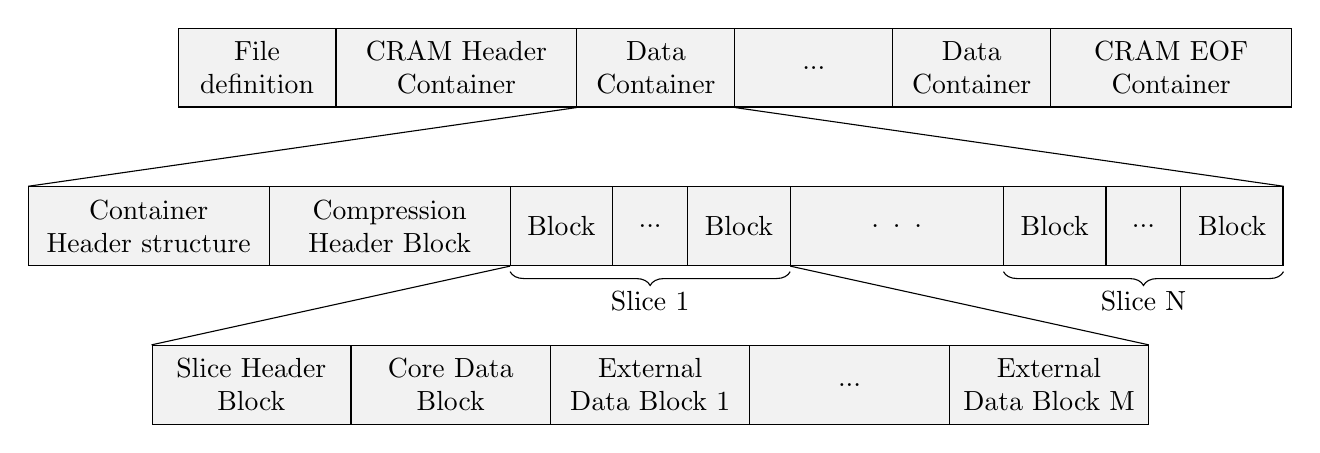
\begin{tikzpicture}[
  every node/.style={scale=1.0},
  boxes/.style={rectangle split,rectangle split parts=#1,draw,rectangle split horizontal,text width=5em,align=center,minimum height=1cm,fill=black!5,on grid},
  notes/.style={text width=20em,align=center,minimum height=1cm,on grid},
]
\node (file) [boxes=6] {
\nodepart{one}File definition
\nodepart[text width=8em]{two}CRAM Header Container
\nodepart{three}Data Container
\nodepart{four}...
\nodepart{five}Data Container
\nodepart[text width=8em]{six}CRAM EOF Container
};

\node (container) [boxes=9,below=1 of file.three south,text width=8em] {
\nodepart{one}Container Header structure
\nodepart{two}Compression Header Block
\nodepart[text width=3em]{three}Block
\nodepart[text width=2em]{four}...
\nodepart[text width=3em]{five}Block
\nodepart[text width=7em]{six}. . .
\nodepart[text width=3em]{seven}Block
\nodepart[text width=2em]{eight}...
\nodepart[text width=3em]{nine}Block
};
\draw (file.two split south) to (container.north west);
\draw (file.three split south) to (container.north east);

\draw[decoration={brace,mirror,amplitude=5pt,raise=2pt},decorate]
  (container.two split south) to (container.five split south);
\node [below=0.2 of container.four south] {Slice 1};

\draw[decoration={brace,mirror,amplitude=5pt,raise=2pt},decorate]
  (container.six split south) to (container.south east);
\node [below=0.2 of container.eight south] {Slice N};

\node (slice) [boxes=5,below=1 of container.four south, text width=6.5em] {
\nodepart{one}Slice Header Block
\nodepart{two}Core Data Block
\nodepart{three}External Data Block 1
\nodepart{four}...
\nodepart{five}External Data Block M
};
\draw (container.two split south) to (slice.north west);
\draw (container.five split south) to (slice.north east);
\end{tikzpicture}

Figure 4: Slices formed from a series of concatenated blocks
\end{center}

\section{\textbf{File definition}}

Each CRAM file starts with a fixed length (26 bytes) definition with the following 
fields:

\begin{tabular}{|l|l|l|}
\hline
\textbf{Data type} & \textbf{Name} & \textbf{Value}\tabularnewline
\hline
byte[4] & format magic number & CRAM (0x43 0x52 0x41 0x4d)\tabularnewline
\hline
unsigned byte & major format number & 3 (0x3)\tabularnewline
\hline
unsigned byte & minor format number & 1 (0x1)\tabularnewline
\hline
byte[20] & file id & CRAM file identifier (e.g. file name or SHA1 checksum)\tabularnewline
\hline
\end{tabular}

Valid CRAM \textit{major}.\textit{minor} version numbers are as follows:

\begin{itemize}
\item[\textit{1.0}]
The original public CRAM release.

\item[\textit{2.0}]
The first CRAM release implemented in both Java and C; tidied up
implementation vs specification differences in \textit{1.0}.

\item[\textit{2.1}]
Gained end of file markers; compatible with \textit{2.0}.

\item[\textit{3.0}]
Additional compression methods; header and data checksums;
improvements for unsorted data.

\item[\textit{3.1}]
Additional EXTERNAL compression codecs only.
\end {itemize}

CRAM 3.0 and 3.1 differ only in the list of compression
methods available, so tools that output CRAM 3 without using any 3.1
codecs should write the header to indicate 3.0 in order to permit
maximum compatibility.

\section{\textbf{Container header structure}}
\label{sec:container}

The file definition is followed by one or more containers with the following header 
structure where the container content is stored in the `blocks' field:

\begin{tabular}{|l|>{\raggedright}p{120pt}|>{\raggedright}p{260pt}|}
\hline
\textbf{Data type} & \textbf{Name} & \textbf{Value}
\tabularnewline
\hline
int32 & length & the sum of the lengths of all blocks in this container (headers and data); 
equal to the total byte length of the container minus the byte length of this header structure\tabularnewline
\hline
itf8 & reference sequence id & reference sequence identifier  or\linebreak{}
-1 for unmapped reads\linebreak{}
-2 for multiple reference sequences.\linebreak{}
All slices in this container must have a reference sequence id matching this value.\tabularnewline
\hline
itf8 & starting position on the reference & the alignment start position\tabularnewline
\hline
itf8 & alignment span & the length of the alignment\tabularnewline
\hline
itf8 & number of records & number of records in the container\tabularnewline
\hline
ltf8 & record counter & 1-based sequential index of records in the file/stream.\tabularnewline
\hline
ltf8 & bases & number of read bases\tabularnewline
\hline
itf8 & number of blocks & the total number of blocks in this container\tabularnewline
\hline
array\texttt{<}itf8\texttt{>} & landmarks & the locations of slices in this container as byte offsets from the end of
this container header, used for random access indexing.
For sequence data containers, the landmark count must equal the slice count.\linebreak{}
Since the block before the first slice is the compression header,
landmarks[0] is equal to the byte length of the compression header.\tabularnewline
\hline
int & crc32 & CRC32 hash of the all the preceding bytes in the container.\tabularnewline
\hline
byte[ ] & blocks & The blocks contained within the container.\tabularnewline
\hline
\end{tabular}

In the initial CRAM header container, the reference sequence id,
starting position on the reference, and alignment span fields must be
ignored when reading. The landmarks array is optional for the CRAM
header, but if it exists it should point to block offsets instead of
slices, with the first block containing the textual header.

In data containers specifying unmapped reads or multiple reference
sequences (i.e. reference sequence id $< 0$), the starting position on
the reference and alignment span fields must be ignored when
reading. When writing, it is recommended to set each of these ignored
fields to the value 0.


\subsection{\textbf{CRAM header container}}
\label{subsec:cram-header-container}

The first container in a CRAM file contains a textual header in one or more blocks.  See section~\ref{subsec:header-block} for more details on the layout of data within these blocks and constraints applied to the contents of the SAM header.

The landmarks field of the container header structure may be used to
indicate the offsets of the blocks used in the header container.
These may optionally be omitted by specifying an array size of zero.

\section{\textbf{Block structure}}
\label{sec:block-struct}

Containers consist of one or more blocks. Block compression is applied independently 
and in addition to any encodings used to compress data within the block. The block 
have the following header structure with the data stored in the `block data' field:

\begin{tabular}{|l|>{\raggedright}p{120pt}|>{\raggedright}p{260pt}|}
\hline
\textbf{Data type} & \textbf{Name} & \textbf{Value}
\tabularnewline
\hline
byte & method & the block compression method (and first CRAM version): \linebreak{}
0: raw (none)*\linebreak{}
1: gzip\linebreak{}
2: bzip2 (v2.0)\linebreak{}
3: lzma (v3.0)\linebreak{}
4: rans4x8 (v3.0)\linebreak{}
5: rans4x16 (v3.1)\linebreak{}
6: adaptive arithmetic coder (v3.1)\linebreak{}
7: fqzcomp (v3.1)\linebreak{}
8: name tokeniser (v3.1)
\tabularnewline
\hline
byte & block content type id & the block content type identifier\tabularnewline
\hline
itf8 & block content id & the block content identifier used to associate external 
data blocks with data series\tabularnewline
\hline
itf8 & size in bytes* & size of the block data after applying block compression\tabularnewline
\hline
itf8 & raw size in bytes* & size of the block data before applying block compression\tabularnewline
\hline
byte[ ] & block data & the data stored in the block:\linebreak{}
$\bullet$ bit stream of CRAM records (core data block)\linebreak{}
$\bullet$ byte stream (external data block)\linebreak{}
$\bullet$ additional fields ( header blocks)\tabularnewline
\hline
byte[4] & CRC32 & CRC32 hash value for all preceding bytes in the block\tabularnewline
\hline
\end{tabular}

* Note on raw method: both compressed and raw sizes must be set to the same value.

Empty blocks may occur in the files.
Blocks with a raw (uncompressed) size of zero are treated as empty,
irrespective of their ``method'' byte.  This is equivalent to
interpreting them as having method zero (raw) and compressed size of
zero.

\subsection{\textbf{Block content types}}

CRAM has the following block content types:

\begin{threeparttable}[t]
\begin{tabular}{|>{\raggedright}p{143pt}|>{\raggedright}p{45pt}|>{\raggedright}p{116pt}|>{\raggedright}p{114pt}|}
\hline
\textbf{Block content type} & \textbf{Block content type id} & \textbf{Name} & \textbf{Contents}\tabularnewline
\hline
FILE\_HEADER & 0 & CRAM header block & CRAM header\tabularnewline
\hline
COMPRESSION\_HEADER & 1 & Compression header block & See specific section\tabularnewline
\hline
SLICE\_HEADER\tnote{a} & 2 & Slice header block & See specific section\tabularnewline
\hline
 & 3 &  & reserved\tabularnewline
\hline
EXTERNAL\_DATA & 4 & external data block & data produced by external encodings\tabularnewline
\hline
CORE\_DATA & 5 & core data block & bit stream of all encodings except for external encodings\tabularnewline
\hline
\end{tabular}
\begin{tablenotes}
\item[a] Formerly MAPPED\_SLICE\_HEADER.  Now used by all slice headers regardless of mapping status.
\end{tablenotes}
\end{threeparttable}

\subsection{\textbf{Block content id}}

Block content id is used to distinguish between external blocks in the same slice. 
Each external encoding has an id parameter which must be one of the external block 
content ids. For external blocks the content id is a positive integer. For all 
other blocks content id should be 0. Consequently, all external encodings must 
not use content id less than 1. 

\subsubsection*{Data blocks}

Data is stored in data blocks. There are two types of data blocks: core data blocks 
and external data blocks.The difference between core and external data blocks is 
that core data blocks consist of data series that are compressed using bit encodings 
while the external data blocks are byte compressed. One core data block and any 
number of external data blocks are associated with each slice.

Writing to and reading from core and external data blocks is organised through 
CRAM records. Each data series is associated with an encoding. In case of external 
encodings the block content id is used to identify the block where the data series 
is stored. Please note that external blocks can have multiple data series associated 
with them; in this case the values from these data series will be interleaved. 


\subsection{\textbf{CRAM header block(s)}}
\label{subsec:header-block}

The SAM header is stored in the first block of the CRAM header container (see section~\ref{subsec:cram-header-container}).
This block may be uncompressed or gzip compressed only.
This block is followed by zero or more uncompressed expansion blocks.
If present, these permit in-place editing of the CRAM header, allowing it to grow or shrink with a compensatory size change applied to the subsequence expansion block, avoiding the need to rewrite the remainder of the file.
The contents of any expansion blocks should be zero bytes (nul characters).

The format of the initial SAM header block is a 32-bit little-endian integer holding the length of the text of the SAM header, minus nul-termination bytes, followed by the text itself.
Although 32-bit, the maximum permitted value is $2^{31}$, and all lengths must be positive.

The following constraints apply to the SAM header text: 

\begin{itemize}
\item The SQ:MD5 checksum is required unless the reference sequence has been embedded 
into the file.
\end{itemize}

\subsection{\textbf{Compression header block}}
\label{subsec:compression-header}

The compression header block consists of 3 parts: preservation map, data series 
encoding map and tag encoding map.

\subsubsection*{Preservation map}

The preservation map contains information about which data was preserved in the 
CRAM file. It is stored as a map with byte[2] keys:

\begin{tabular}{|l|l|>{\raggedright}p{100pt}|>{\raggedright}p{220pt}|}
\hline
\textbf{Key} & \textbf{Value data type} & \textbf{Name} & \textbf{Value}\tabularnewline
\hline
RN & bool & read names included & true if read names are preserved for all reads\tabularnewline
\hline
AP & bool & AP data series delta & true if AP data series is delta, false otherwise\tabularnewline
\hline
RR & bool & reference required & true if reference sequence is required to restore 
the data completely\tabularnewline
\hline
SM & byte[5] & substitution matrix & substitution matrix\tabularnewline
\hline
TD & array\texttt{<}byte\texttt{>} & tag ids dictionary & a list of lists of tag ids, see tag encoding section\tabularnewline
\hline
\end{tabular}

The boolean values are optional, defaulting to true when absent, although it is recommended to explicitly set them.  SM and TD are mandatory.

\subsubsection*{Data series encodings}

Each data series has an encoding. These encoding are stored in a map with byte[2] 
keys and are decoded in approximately this order\footnote{The precise order is defined in section~\ref{sec:record}.}:

\begin{threeparttable}[t]
\begin{tabular}{|l|l|>{\raggedright}p{100pt}|>{\raggedright}p{220pt}|}
\hline
\textbf{Key} & \textbf{Value data type} & \textbf{Name} & \textbf{Value}\tabularnewline
\hline
BF & encoding\texttt{<}int\texttt{>} & BAM bit flags & see separate section\tabularnewline
\hline
CF & encoding\texttt{<}int\texttt{>} & CRAM bit flags & see specific section\tabularnewline
\hline
RI & encoding\texttt{<}int\texttt{>} & reference id & record reference id from
the SAM file header\tabularnewline
\hline
RL & encoding\texttt{<}int\texttt{>} & read lengths & read lengths\tabularnewline
\hline
AP & encoding\texttt{<}int\texttt{>} & in-seq positions & if \textbf{AP-Delta} = true: 0-based alignment start
delta from the AP value in the previous record.
Note this delta may be negative, for example when switching references in a multi-reference slice.
When the record is the first in the slice, the previous position used is the slice alignment-start field (hence the first delta should be zero for single-reference slices, or the AP value itself for multi-reference slices).  \linebreak{}
if \textbf{AP-Delta} = false: encodes the alignment start position directly\tabularnewline
\hline
RG & encoding\texttt{<}int\texttt{>} & read groups & read groups. Special value 
`-1' stands for no group.\tabularnewline
\hline
RN\tnote{a} & encoding\texttt{<}byte[ ]\texttt{>} & read names & read names\tabularnewline
\hline
MF & encoding\texttt{<}int\texttt{>} & next mate bit flags & see specific section\tabularnewline
\hline
NS & encoding\texttt{<}int\texttt{>} & next fragment reference sequence id & reference 
sequence ids for the next fragment \tabularnewline
\hline
NP & encoding\texttt{<}int\texttt{>} & next mate alignment start & alignment positions 
for the next fragment\tabularnewline
\hline
TS & encoding\texttt{<}int\texttt{>} & template size & template sizes\tabularnewline
\hline
NF & encoding\texttt{<}int\texttt{>} & distance to next fragment & number of records
to skip to the next fragment\tnote{b}\tabularnewline
\hline
TL\tnote{c} & encoding\texttt{<}int\texttt{>} & tag ids  & list of tag ids, see tag encoding
section\tabularnewline
\hline
FN & encoding\texttt{<}int\texttt{>} & number of read features & number of read
features in each record\tabularnewline
\hline
FC & encoding\texttt{<}byte\texttt{>} & read features codes & see separate section\tabularnewline
\hline
FP & encoding\texttt{<}int\texttt{>} & in-read positions & positions of the read
features\tabularnewline
\hline
DL & encoding\texttt{<}int\texttt{>} & deletion lengths & base-pair deletion lengths\tabularnewline
\hline
BB & encoding\texttt{<}byte[ ]\texttt{>} & stretches of bases & bases\tabularnewline
\hline
QQ & encoding\texttt{<}byte[ ]\texttt{>} & stretches of quality scores & quality scores\tabularnewline
\hline
BS & encoding\texttt{<}byte\texttt{>} & base substitution codes & base substitution
codes\tabularnewline
\hline
IN & encoding\texttt{<}byte[ ]\texttt{>} & insertion & inserted bases\tabularnewline
\hline
RS & encoding\texttt{<}int\texttt{>} & reference skip length & number of skipped 
bases for the `N' read feature\tabularnewline
\hline
PD & encoding\texttt{<}int\texttt{>} & padding & number of padded bases\tabularnewline
\hline
HC & encoding\texttt{<}int\texttt{>} & hard clip & number of hard clipped bases\tabularnewline
\hline
SC & encoding\texttt{<}byte[ ]\texttt{>} & soft clip & soft clipped bases\tabularnewline
\hline
MQ & encoding\texttt{<}int\texttt{>} & mapping qualities & mapping quality scores\tabularnewline
\hline
BA & encoding\texttt{<}byte\texttt{>} & bases & bases\tabularnewline
\hline
QS & encoding\texttt{<}byte\texttt{>} & quality scores & quality scores\tabularnewline
\hline
TC\tnote{d} & N/A & legacy field & to be ignored\tabularnewline
\hline
TN\tnote{d} & N/A & legacy field & to be ignored\tabularnewline
\end{tabular}

\begin{tablenotes}
\item[a] Note RN this is decoded after MF if the record is detached from the mate and we are attempting to auto-generate read names.
\item[b] The count is reset for each slice so NF can only refer to a record later within this slice.
\item[c] TL is followed by decoding the tag values themselves, in order of appearance in the tag dictionary.
\item[d] TC and TN are legacy data series from CRAM 1.0.
They have no function in CRAM 3.0 and should not be present.
However some implementations do output them and decoders must silently skip these fields.
It is illegal for TC and TN to contain any data values, although there
may be empty blocks associated with them.
\end{tablenotes}
\end{threeparttable}

\subsubsection*{Tag encodings}
\label{subsubsec:tags}

The tag dictionary (TD) describes the unique combinations of tag id / type that occur on each alignment record.
For example if we search the id / types present in each record and find only two combinations -- X1:i BC:Z SA:Z: and X1:i: BC:Z -- then we have two dictionary entries in the TD map.

Let $L_{i}=\{T_{i0}, T_{i1}, \ldots, T_{ix}\}$ be a list of all tag ids for a record $R_{i}$, where $i$ is the sequential record index and $T_{ij}$ denotes $j$-th tag id in the record.
The list of unique $L_{i}$ is stored as the TD value in the preservation map.
Maintaining the order is not a requirement for encoders (hence ``combinations''), but it is permissible and thus different permutations, each encoded with their own elements in TD, should be supported by the decoder.
Each $L_{i}$ element in TD is assigned a sequential integer number starting with 0.
These integer numbers are referred to by the TL data series.
Using TD, an integer from the TL data series can be mapped back into a list of tag ids.
Thus per alignment record we only need to store tag values and not their ids and types.

The TD is written as a byte array consisting of $L_{i}$ values separated with \textbackslash{}0.
Each $L_{i}$ value is written as a concatenation of 3 byte $T_{ij}$ elements: tag id followed by BAM tag type code (one of A, c, C, s, S, i, I, f, F, Z, H or B, as described in the SAM specification).
For example the TD for tag lists X1:i BC:Z SA:Z and X1:i BC:Z may be encoded as X1CBCZSAZ\textbackslash{}0X1CBCZ\textbackslash{}0, with X1C indicating a 1 byte unsigned value for tag X1.

\subsubsection*{Tag values}

The encodings used for different tags are stored in a map.
The key is 3 bytes formed from the BAM tag id and type code, matching the TD dictionary described above.
Unlike the Data Series Encoding Map, the key is stored in the map as an ITF8 encoded integer, constructed using $(char1<<16) + (char2<<8) + type$.
For example, the 3-byte representation of OQ:Z is \{0x4F, 0x51, 0x5A\} and these bytes are interpreted as the integer key 0x004F515A, leading to an ITF8 byte stream \{0xE0, 0x4F, 0x51, 0x5A\}.

\begin{tabular}{|l|l|l|>{\raggedright}p{160pt}|}
\hline
\textbf{Key} & \textbf{Value data type} & \textbf{Name} & \textbf{Value}
\tabularnewline
\hline
TAG ID 1:TAG TYPE 1 & encoding\texttt{<}byte[ ]\texttt{>} & read tag 1 & tag values
(names and types are available in the data series code)\tabularnewline
\hline
... &  & ... & ...\tabularnewline
\hline
TAG ID N:TAG TYPE N & encoding\texttt{<}byte[ ]\texttt{>} & read tag N & ...\tabularnewline
\hline
\end{tabular}

Note that tag values are encoded as array of bytes. The routines to convert tag 
values into byte array and back are the same as in BAM with the exception of value 
type being captured in the tag key rather in the value.
Hence consuming 1 byte for types `C' and `c', 2 bytes for types `S' and `s', 4 bytes for types `I', `i' and `f', and a variable number of bytes for types `H', `Z' and `B'.

\subsection{\textbf{Slice header block}}

The slice header block is never compressed (block method=raw). For reference mapped 
reads the slice header also defines the reference sequence context of the data 
blocks associated with the slice. Mapped reads can be stored along with
\textbf{placed unmapped}\footnote{Unmapped reads can be \textit{placed} or \textit{unplaced}.
By placed unmapped read we mean a read that is unmapped according to bit 0x4 of the
BF (BAM bit flags) data series, but has position fields filled in, thus "placing"  it on a reference sequence. In contrast,
unplaced unmapped reads have have a reference sequence ID of -1 and alignment position of 0.}
reads on the same reference within the same slice.

Slices with the Multiple Reference flag (-2) set as the sequence ID in the header may contain reads
mapped to multiple external references, including unmapped\footnotemark[\value{footnote}] reads (placed on these references or unplaced),
but multiple embedded references cannot be combined in this way.  When multiple references are
used, the RI data series will be used to determine the reference sequence ID for each record.  This
data series is not present when only a single reference is used within a slice.

The Unmapped (-1) sequence ID in the header is for slices containing only unplaced
unmapped\footnotemark[\value{footnote}] reads.

A slice containing data that does not use the external reference in
any sequence may set the reference MD5 sum to zero.  This can happen
because the data is unmapped or the sequence has been stored verbatim
instead of via reference-differencing.  This latter scenario is
recommended for unsorted or non-coordinate-sorted data.

The slice header block contains the following fields.

\begin{tabular}{|l|l|>{\raggedright}p{200pt}|}
\hline
\textbf{Data type} & \textbf{Name} & \textbf{Value}\tabularnewline
\hline
itf8 & reference sequence id & reference sequence identifier or\linebreak{}
-1 for unmapped reads\linebreak{}
-2 for multiple reference sequences.\linebreak{}
This value must match that of its enclosing container.\tabularnewline
\hline
itf8 & alignment start & the alignment start position\tabularnewline
\hline
itf8 & alignment span & the length of the alignment\tabularnewline
\hline
itf8 & number of records & the number of records in the slice\tabularnewline
\hline
ltf8 & record counter & 1-based sequential index of records in the file/stream\tabularnewline
\hline
itf8 & number of blocks & the number of blocks in the slice\tabularnewline
\hline
itf8[ ] & block content ids & block content ids of the blocks in the slice\tabularnewline
\hline
itf8 & embedded reference bases block content id & block content id for the embedded 
reference sequence bases or -1 for none\tabularnewline
\hline
byte[16] & reference md5 & MD5 checksum of the reference bases within the slice 
boundaries.  If this slice has reference sequence id of -1 (unmapped) or -2 (multi-ref)
the MD5 should be 16 bytes of \textbackslash{}0. For embedded references, the MD5
can either be all-zeros or the MD5 of the embedded sequence.\tabularnewline
\hline
byte[ ] & optional tags & a series of tag,type,value tuples encoded as
per BAM auxiliary fields.\tabularnewline
\hline
\end{tabular}

The alignment start and alignment span values should only be utilised
during decoding if the slice has mapped data aligned to a single
reference (reference sequence id $>= 0$).  For multi-reference slices
or those with unmapped data, it is recommended to fill these fields
with value 0.

The optional tags are encoded in the same manner as BAM tags.  I.e. a
series of binary encoded tags concatenated together where each tag
consists of a 2 byte key (matching [A-Za-z][A-Za-z0-9]) followed by a
1 byte type ([AfZHcCsSiIB]) followed by a string of bytes in a format
defined by the type.

Tags starting in a capital letter are reserved while lowercase ones or
those starting with X, Y or Z are user definable.  Any tag not
understood by a decoder should be skipped over without producing an
error.

At present no tags are defined.

% Details omitted until we fully work through all the corner cases,
% such as seq/qual of *.
%
% Reserved tags are defined as follows:
% 
% \begin{tabular}{|l|l|>{\raggedright}p{325pt}|}
% \hline
% \textbf{Tag type} & \textbf{BAM format} & \textbf{Meaning}\tabularnewline
% \hline
% BD & i & Sum over all reads of the CRC32 hash of sequence base.  This
% may be used to validate round-trips in and out of CRAM.
% calls\tabularnewline
% \hline
% SD & i & Sum over all reads of the CRC32 hash of quality scores. (If
% the quality string is ``*'' in SAM then the hash is of the BAM encoded
% version - a string of bytes with value 255.)\tabularnewline
% \hline
% \end{tabular}


\subsection{\textbf{Core data block}}

A core data block is a bit stream (most significant bit first) consisting of data from one 
or more CRAM records. Please note that one byte could hold more then one CRAM record 
as a minimal CRAM record could be just a few bits long. The core data block has 
the following fields:

\begin{tabular}{|l|>{\raggedright}p{120pt}|>{\raggedright}p{260pt}|}
\hline
\textbf{Data type} & \textbf{Name} & \textbf{Value}
\tabularnewline
\hline
bit[ ] & CRAM record 1 & The first CRAM record\tabularnewline
\hline
... & ... & ...\tabularnewline
\hline
bit[ ] & CRAM record N & The Nth CRAM record \tabularnewline
\hline
\end{tabular}

\subsection{\textbf{External data blocks}}

The relationship between the core data block and external data blocks is shown in the following 
picture: 

\begin{center}
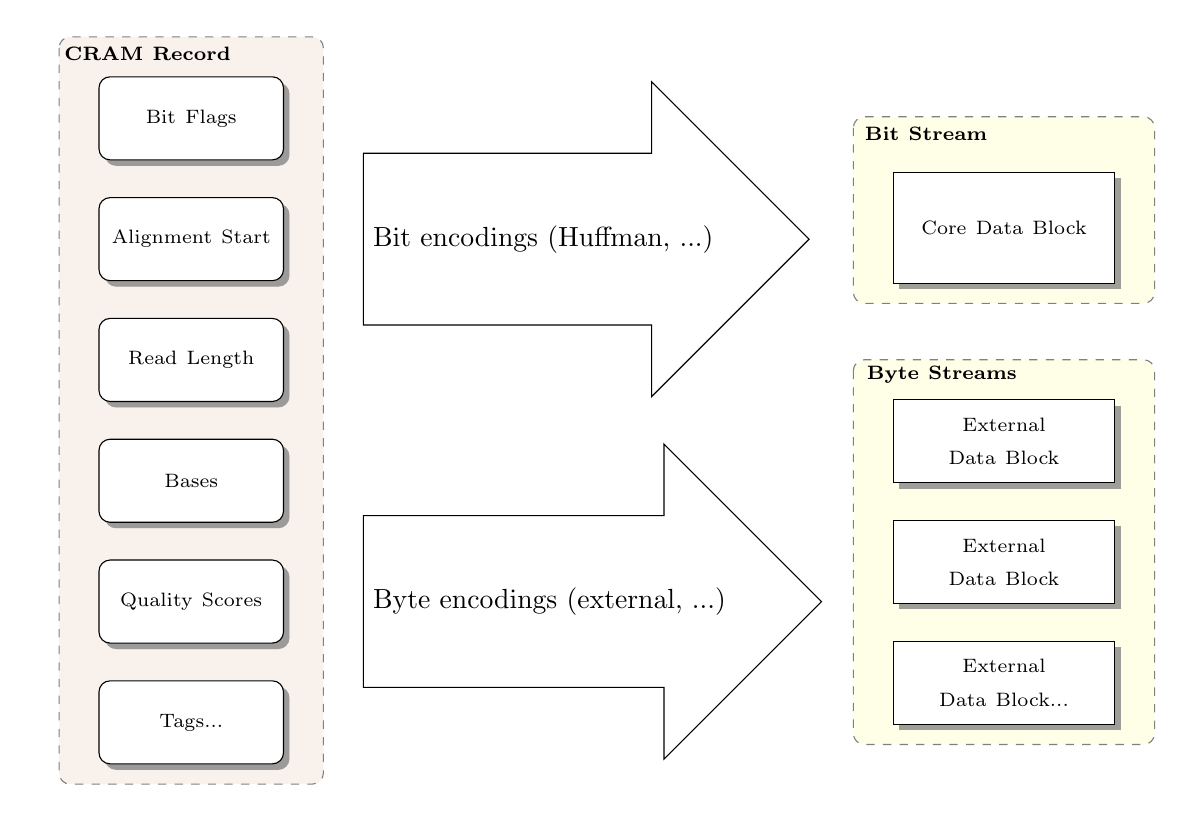
\begin{tikzpicture}

\usetikzlibrary{shapes, shadows, positioning, arrows,  decorations.markings}

\pgfdeclarelayer{background}
\pgfsetlayers{background,main}

\tikzstyle{dsbox} = [blockbox, text width=6em, minimum width=6em, minimum height=3em, rounded corners, drop shadow]
\tikzstyle{blockbox}=[draw, fill=white, text width=4.0em, text centered, minimum height=1.0em, drop shadow]
\tikzstyle{encodedblocklarge} = [blockbox, text width=6em, minimum width=8em, minimum height=4em, drop shadow]
\tikzstyle{encodedblock} = [blockbox, text width=6em, minimum width=8em, minimum height=3em, drop shadow]

\tikzstyle{texto} = [above, text width=8em, text centered]

\newcommand{\cramRecord}[6]{%
\begin{pgfonlayer}{background}
    \path (#1.west |- #1.north) + (-0.5, 0.5) node (a1) {};
    \path (#1.east |- #6.south) + (+0.5,-0.25) node (a2) {};
    \path[fill=brown!10,rounded corners, draw=black!50, dashed]
      (a1) rectangle (a2);
    \path (a1.east |- a1.south) + (1.0,-0.3) node[texto]
      {\scriptsize\textbf{CRAM Record}};
\end{pgfonlayer}}

\newcommand{\dsbox}[2]{node (p#1) [dsbox]
{\scriptsize{#2}}}
\newcommand{\encodedblock}[2]{node (p#1) [encodedblock]
	{\scriptsize{#2}}}
\newcommand{\encodedblocklarge}[2]{node (p#1) [encodedblocklarge]
   {\scriptsize{#2}}}

\path +(-2.5,-1.5) \dsbox{1}{Bit Flags};
\path (p1.south)+(0.0,-1.0) \dsbox{2}{Alignment Start};
\path (p2.south)+(0.0,-1.0) \dsbox{3}{Read Length};
\path (p3.south)+(0.0,-1.0) \dsbox{4}{Bases};
\path (p4.south)+(0.0,-1.0) \dsbox{5}{Quality Scores};
\path (p5.south)+(0.0,-1.0) \dsbox{6}{Tags...};

\cramRecord{p1}{p2}{p3}{p4}{p5}{p6}

\newcommand{\blockStreams}[4]{%
\begin{pgfonlayer}{background}
    \path (#1.west |- #1.north)+(-0.5, .7) node (a1) {};
    \path (#1.east |- #1.south)+(+0.5, -0.25) node (a2) {};
    \path (#2.west |- #2.north)+(-0.5, 0.5) node (a3) {};
    \path (#4.east |- #4.south)+(+0.5, -0.25) node (a4) {};
    \path[fill=yellow!10, rounded corners, draw=black!50, dashed]
      (a1) rectangle (a2);
    \path (a1.east |- a1.south)+(0.8,-0.3) node[texto]
      {\scriptsize\textbf{Bit Stream}};
    \path[fill=yellow!10, rounded corners, draw=black!50, dashed]
      (a3) rectangle (a4);
    \path (a3.east |- a3.south)+(1.0,-0.3) node[texto]{\scriptsize\textbf{Byte Streams}};
\end{pgfonlayer}}

\path (a1.south) + (12.0, -2.3) \encodedblocklarge {7} {Core Data Block};
\path (p7.south) + (0.0, -2.0) \encodedblock {8} {External Data Block};
\path (p8.south) + (0.0, -1.0) \encodedblock {9} {External Data Block}; 
\path (p9.south) + (0.0, -1.0) \encodedblock {10}{External Data Block...};

\blockStreams {p7} {p8} {p9} {p10}

\node[minimum size=4cm, right = of p2, single arrow, draw, single arrow head indent=0ex, black] {Bit encodings (Huffman, ...) };

\node[minimum size=4cm, right = of p5, single arrow, draw, single arrow head indent=0ex, black] {Byte encodings (external, ...) };

\end{tikzpicture}

Figure 5: The relationship between core and external encodings, and core and external data blocks.

\end{center}

The picture shows how a CRAM record (on the left) is distributed between the core 
data block and one or more external data blocks, via core or external encodings. The specific 
encodings presented are only examples for purposes of illustration. The main point is 
to distinguish between core bit encodings whose output is always stored in a core data 
block, and external byte encodings whose output is always stored in external data 
blocks.

\section{\textbf{End of file container}}

A special container is used to mark the end of a file or stream. It is required in version 3 or later. The idea is to provide an easy and a quick way to detect that a CRAM file or stream is complete. The marker is basically an empty container with ref seq id set to -1 (unaligned) and alignment 
start set to 4542278.

Here is a complete content of the EOF container explained in detail:

\begin{tabular}{|l|l|>{\raggedright}p{150pt}|>{\raggedright}p{180pt}|}
\hline
\textbf{hex bytes} & \textbf{data type} & \textbf{decimal value} & \textbf{field 
name}\tabularnewline
\hline
\multicolumn{4}{|l|}{\textit{Container header}}\tabularnewline
\hline
0f 00 00 00 & integer & 15 & size of blocks data\tabularnewline
\hline
ff ff ff ff 0f & itf8 & -1 & ref seq id\tabularnewline
\hline
e0 45 4f 46 & itf8 & 4542278 & alignment start\tabularnewline
\hline
00 & itf8 & 0 & alignment span\tabularnewline
\hline
00 & itf8 & 0 & number of records\tabularnewline
\hline
00 & itf8 & 0 & global record counter\tabularnewline
\hline
00 & itf8 & 0 & bases\tabularnewline
\hline
01 & itf8 & 1 & block count\tabularnewline
\hline
00 & array & 0 & landmarks\tabularnewline
\hline
05 bd d9 4f & integer & 1339669765 & container header CRC32\tabularnewline
\hline
\multicolumn{4}{|l|}{\textit{Compression header block}}\tabularnewline
\hline
00 & byte & 0 (RAW) & compression method\tabularnewline
\hline
01 & byte & 1 (COMPRESSION\_HEADER) & block content type\tabularnewline
\hline
00 & itf8 & 0 & block content id\tabularnewline
\hline
06 & itf8 & 6 & compressed size\tabularnewline
\hline
06 & itf8 & 6 & uncompressed size\tabularnewline
\hline
\multicolumn{4}{|l|}{\textit{Compression header}}\tabularnewline
\hline
01 & itf8 & 1 & preservation map byte size\tabularnewline
\hline
00 & itf8 & 0 & preservation map size\tabularnewline
\hline
01 & itf8 & 1 & encoding map byte size\tabularnewline
\hline
00 & itf8 & 0 & encoding map size\tabularnewline
\hline
01 & itf8 & 1 & tag encoding byte size\tabularnewline
\hline
00 & itf8 & 0 & tag encoding map size\tabularnewline
\hline
ee 63 01 4b & integer & 1258382318 & block CRC32\tabularnewline
\hline
\end{tabular}

When compiled together the EOF marker is 38 bytes long and in hex representation 
is:

0f 00 00 00 ff ff ff ff 0f e0 45 4f 46 00 00 00 00 01 00 05 bd d9 4f 00 01 00 06 06 01 00 01 00 01 00 ee 63 01 4b

\section{\textbf{Record structure}}
\label{sec:record}

CRAM record is based on the SAM record but has additional features allowing for 
more efficient data storage.  In contrast to BAM record CRAM record uses bits as 
well as bytes for data storage. This way, for example, various coding techniques 
which output variable length binary codes can be used directly in CRAM. On the 
other hand, data series that do not require binary coding can be stored separately 
in external blocks with some other compression applied to them independently.

As CRAM data series may be interleaved within the same blocks\footnote{Interleaving can sometimes provide better compression, however it also adds dependency between types of data meaning it is not possible to selectively decode one data series if it co-locates with another data series in the same block.} understanding the order in which CRAM data series must be decoded is vital.

The overall flowchart is below, with more detailed description in the subsequent sections.

\algnewcommand\algorithmicto{\text{ \textbf{to} }}

\subsection{\textbf{CRAM record}}

Both mapped and unmapped reads start with the following fields. Please note that 
the data series type refers to the logical data type and the data series name corresponds 
to the data series encoding map.

\begin{tabular}{|>{\raggedright}p{70pt}|>{\raggedright}p{75pt}|>{\raggedright}p{90pt}|>{\raggedright}p{171pt}|}
\hline
\textbf{Data series type} & \textbf{Data series name} & \textbf{Field} & \textbf{Description}\tabularnewline
\hline
int & BF & BAM bit flags & see BAM bit flags below\tabularnewline
\hline
int & CF & CRAM bit flags & see CRAM bit flags below\tabularnewline
\hline
- & - & Positional data & See section \ref{subsec:positions}\tabularnewline
\hline
- & - & Read names & See section \ref{subsec:names}\tabularnewline
\hline
- & - & Mate records & See section \ref{subsec:mate}\tabularnewline
\hline
- & - & Auxiliary tags & See section \ref{subsec:tags}\tabularnewline
\hline
- & - & Sequences & See sections \ref{subsec:mapped} and \ref{subsec:unmapped}\tabularnewline
\hline
\end{tabular}

\subsubsection*{\textbf{BAM bit flags (BF data series)}}

The following flags are duplicated from the SAM and BAM specification, with identical meaning.
Note however some of these flags can be derived during decode, so may be omitted in the CRAM file and the bits computed based on both reads of a pair-end library residing within the same slice.

\begin{threeparttable}[t]
\begin{tabular}{|>{\raggedright}p{144pt}|>{\raggedright}p{144pt}|>{\raggedright}p{144pt}|}
\hline
\textbf{Bit flag} & \textbf{Comment} & \textbf{Description}\tabularnewline
\hline
0x1 &  & template having multiple segments in sequencing\tabularnewline
\hline
0x2 &  & each segment properly aligned according to the aligner\tabularnewline
\hline
0x4 &  & segment unmapped\tnote{a}\tabularnewline
\hline
0x8 & calculated\tnote{b}\ \ or stored in the mate's info & next segment in template unmapped\tabularnewline
\hline
0x10 &  & SEQ being reverse complemented\tabularnewline
\hline
0x20 & calculated\tnote{b}\ \ or stored in the mate's info & SEQ of the next segment in the
template being reverse complemented\tabularnewline
\hline
0x40 &  & the first segment in the template\tnote{c}\tabularnewline
\hline
0x80 &  & the last segment in the template\tnote{c}\tabularnewline
\hline
0x100 &  & secondary alignment\tabularnewline
\hline
0x200 &  & not passing quality controls\tabularnewline
\hline
0x400 &  & PCT or optical duplicate\tabularnewline
\hline
0x800 &  & Supplementary alignment\tabularnewline
\hline
\end{tabular}
\begin{tablenotes}
\item[a] Bit 0x4 is the only reliable place to tell whether the read is unmapped.  If 0x4 is set, no assumptions may be made about bits 0x2, 0x100 and 0x800.
\item[b] For segments within the same slice.
\item[c] Bits 0x40 and 0x80 reflect the read ordering within each template inherent in the sequencing technology used, which may be independent from the actual mapping orientation.
If 0x40 and 0x80 are both set, the read is part of a linear template (one where the template sequence is expected to be in a linear order), but it is neither the first nor the last read.
If both 0x40 and 0x80 are unset, the index of the read in the template is unknown.
This may happen for a non-linear template (such as one constructed by stitching together other templates) or when this information is lost during data processing.
\end{tablenotes}
\end{threeparttable}

\subsubsection*{\textbf{CRAM bit flags (CF data series)}}

The CRAM bit flags (also known as compression bit flags) expressed as an integer represent the CF data series. 
The following compression flags are defined for each CRAM read record:

\begin{tabular}{|>{\raggedright}p{39pt}|>{\raggedright}p{150pt}|>{\raggedright}p{242pt}|}
\hline
\textbf{Bit flag} & \textbf{Name} & \textbf{Description}\tabularnewline
\hline
0x1 & quality scores stored as array & quality scores can be stored as read features
or as an array similar to read bases.\tabularnewline
\hline
0x2 & detached & mate information is stored verbatim (e.g. because the pair spans multiple slices or the fields differ to the CRAM computed method)\tabularnewline
\hline
0x4 & has mate downstream & tells if the next segment should be expected further
in the stream\tabularnewline
\hline
0x8 & decode sequence as ``*'' & informs the decoder that the sequence
is unknown and that any encoded reference differences are present only to
recreate the CIGAR string.\tabularnewline
\hline
\end{tabular}


The following pseudocode describes the general process of decoding an entire CRAM record.
The sequence data itself is in one of two encoding formats depending on whether the record is aligned (mapped).

\subsubsection*{\textbf{Decode pseudocode}}
\newlength{\maxwidth}
\newcommand{\algalign}[2] % #1 = text to left, #2 = text to right
{\makebox[\maxwidth][l]{$#1{}$}${}#2$}

\begin{algorithmic}[1]
\Procedure{DecodeRecord}{}
\settowidth{\maxwidth}{CRAM\_flags\quad}
\State \algalign{BAM\_flags}{\gets}  \Call{ReadItem}{BF, Integer}
\State \algalign{CRAM\_flags}{\gets} \Call{ReadItem}{CF, Integer}
\State \Call{DecodePositions}{}\Comment{See section \ref{subsec:positions}}
\State \Call{DecodeNames}{}\Comment{See section \ref{subsec:names}}
\State \Call{DecodeMateData}{}\Comment{See section \ref{subsec:mate}}
\State \Call{DecodeTagData}{}\Comment{See section \ref{subsec:tags}}
\Statex

\If{$(BF$ AND $4) \ne 0$}\Comment{Unmapped flag}
  \State \Call{DecodeMappedRead}{}\Comment{See section \ref{subsec:mapped}}
\Else
  \State \Call{DecodeUnmappedRead}{}\Comment{See section \ref{subsec:unmapped}}
\EndIf
\EndProcedure
\end{algorithmic}

\subsection{\textbf{CRAM positional data}}
\label{subsec:positions}

Following the bit-wise BAM and CRAM flags, CRAM encodes positional related data including reference, alignment positions and length, and read-group.
Positional data is stored for both mapped and unmapped sequences, as unmapped data may still be ``placed'' at a specific location in the genome (without being aligned).
Typically this is done to keep a sequence pair (paired-end or mate-pair sequencing libraries) together when one of the pair aligns and the other does not.

For reads stored in a position-sorted slice, the AP-delta flag in the compression header preservation map should be set and the AP data series will be delta encoded, using the slice alignment-start value as the first position to delta against.
Note for multi-reference slices this may mean that the AP series includes negative values, such as when moving from an alignment to the end of one reference sequence to the start of the next or to unmapped unplaced data.  When the AP-delta flag is not set the AP data series is stored as a normal integer value.

\begin{tabular}{|>{\raggedright}p{70pt}|>{\raggedright}p{75pt}|>{\raggedright}p{90pt}|>{\raggedright}p{171pt}|}
\hline
\textbf{Data series type} & \textbf{Data series name} & \textbf{Field} & \textbf{Description}\tabularnewline
\hline
int & RI & ref id & reference sequence id (only present in multiref slices)\tabularnewline
\hline
int & RL & read length & the length of the read\tabularnewline
\hline
int & AP & alignment start & the alignment start position\tabularnewline
\hline
int & RG & read group & the read group identifier expressed as the N\textsuperscript{th} record in the header, starting from 0 with -1 for no group\tabularnewline
\hline
\end{tabular}

\vskip 20pt
\begin{algorithmic}[1]
\Procedure{DecodePositions}{}
\If{$slice\_header.reference\_sequence\_id = -2$}
  \State $reference\_id\gets$ \Call{ReadItem}{RI, Integer}
\Else
  \State $reference\_id\gets slice\_header.reference\_sequence\_id$
\EndIf
\State $read\_length \gets$ \Call{ReadItem}{RL, Integer}
\If{$container\_pmap.AP\_delta \ne 0$}
    \If{$first\_record\_in\_slice$}
        \State $last\_position\gets$ $slice\_header.alignment\_start$
    \EndIf
    \State $alignment\_position \gets$ \Call{ReadItem}{AP, Integer} + $last\_position$
    \State $last\_position \gets alignment\_position$
\Else
    \State $alignment\_position \gets$ \Call{ReadItem}{AP, Integer}
\EndIf
\State $read\_group \gets$ \Call{ReadItem}{RG, Integer}
\EndProcedure
\end{algorithmic}

\subsection{Read names (RN data series)}
\label{subsec:names}

Read names can be preserved in the CRAM format, but this is optional and is governed by the \texttt{RN} preservation map key in the container compression header. See section \ref{subsec:compression-header}.
When read names are not preserved the CRAM decoder should generate names, typically based on the file name and a numeric ID of the read using the record counter field of the slice header block.
Note read names may still be preserved even when the \texttt{RN} compression header key indicates otherwise, such as where a read is part of a read-pair and the pair spans multiple slices.
In this situation the record will be marked as detached (see the CF data series) and the mate data below (section \ref{subsec:mate}) will contain the read name.

\begin{tabular}{|>{\raggedright}p{70pt}|>{\raggedright}p{75pt}|>{\raggedright}p{90pt}|>{\raggedright}p{171pt}|}
\hline
\textbf{Data series type} & \textbf{Data series name} & \textbf{Field} & \textbf{Description}\tabularnewline
\hline
byte[ ] & RN & read names & read names\tabularnewline
\hline
\end{tabular}

\vskip 20pt
\begin{algorithmic}[1]
\Procedure{DecodeNames}{}
\If{$container\_pmap.read\_names\_included = 1$}
  \State $read\_name \gets$ \Call{ReadItem}{RN, Byte[]}
\Else
  \State $read\_name \gets$ \Call{GenerateName}{}
\EndIf
\Statex
\EndProcedure
\end{algorithmic}

\subsection{\textbf{Mate records}}
\label{subsec:mate}

There are two ways in which mate information can be preserved in CRAM.
If the next fragment is not in the same slice we store verbatim copies of the insert size, mate reference chromosome and positions, and mate flags (mapped status, orientation) for both records.
In this case both records are labelled as ``detached'' in the CF data series using bit 2.

If this and the next fragment are within the same slice, we can derive much of this information by comparing the two records.
The upstream record has CF bit 4 (mate downstream) flag set and stores the number of records to skip (in the NF data series) between this record and the record for the next fragment on this template, with zero meaning the next fragment is also the next record.
The downstream record has neither CF bits 2 (detached) or 4 (mate downstream) set nor does it use the NF data series (unless it also has an additional ``next fragment'' to refer to).

It is not mandatory to use this deduplication approach and optionally CRAM write implementations may wish to label data as detached even when all records for the template reside in the same slice.
One reason to do this may be to preserve inconsistent data so that it round-trips through the CRAM format with full fidelity

\begin{tabular}{|>{\raggedright}p{68pt}|>{\raggedright}p{115pt}|>{\raggedright}p{228pt}|}
\hline
\textbf{Data series type} & \textbf{Data series name} & \textbf{Description}\tabularnewline
\hline
int & NF & the number of records to skip to the next fragment\tabularnewline
\hline
\end{tabular}

In the above case, the NS (mate reference name), NP (mate position) and TS (template size) fields for both records should be derived once the mate has also been decoded.
Mate reference name and position are obvious and simply copied from the mate.
The template size is computed using the method described in the SAM specification; the inclusive distance from the leftmost to rightmost mapped bases with the sign being positive for the leftmost record and negative for the rightmost record.

If the next fragment is not found within this slice then the following structure is included into the CRAM record.
Note there are cases where read-pairs within the same slice may be marked as detached and use this structure, such as to store mate-pair information that does not match the algorithm used by CRAM for computing the mate data on-the-fly.

\begin{tabular}{|>{\raggedright}p{66pt}|>{\raggedright}p{117pt}|>{\raggedright}p{228pt}|}
\hline
\textbf{Data series type} & \textbf{Data series name} & \textbf{Description}\tabularnewline
\hline
int & MF & next mate bit flags, see table below\tabularnewline
\hline
byte[ ] & RN & the read name (if and only if not known already)\tabularnewline
\hline
int & NS & mate reference sequence identifier \tabularnewline
\hline
int & NP & mate alignment start position \tabularnewline
\hline
int & TS & the size of the template (insert size)\tabularnewline
\hline
\end{tabular}

\subsubsection*{Next mate bit flags (MF data series)}

The next mate bit flags expressed as an integer represent the MF data series.
These represent the missing bits we excluded from the BF data series (when compared to the full SAM/BAM flags).
The following bit flags are defined:

\begin{tabular}{|>{\raggedright}p{47pt}|>{\raggedright}p{134pt}|>{\raggedright}p{250pt}|}
\hline
\textbf{Bit flag} & \textbf{Name} & \textbf{Description}\tabularnewline
\hline
0x1 & mate negative strand bit & the bit is set if the mate is on the negative
strand\tabularnewline
\hline
0x2 & mate unmapped bit & the bit is set if the mate is unmapped\tabularnewline
\hline
\end{tabular}


\subsubsection*{\textbf{Decode mate pseudocode}}

In the following pseudocode we are assuming the current record is $this$ and its mate is $next\_frag$.

\begin{algorithmic}[1]
\Procedure{DecodeMateData}{}
\If{$CF$ AND $2$}\Comment{Detached from mate}
  \State $mate\_flags\gets $ \Call{ReadItem}{MF,Integer}
  \If{$mate\_flags$ AND 1}
    \State $bam\_flags\gets bam\_flags$\ OR\ 0x20\Comment{Mate is reverse-complemented}
  \EndIf
  \If{$mate\_flags$ AND 2}
    \State $bam\_flags\gets bam\_flags$\ OR\ 0x08\Comment{Mate is unmapped}
  \EndIf
  \If{$container\_pmap.read\_names\_included \ne 1$}
    \State $read\_name \gets$ \Call{ReadItem}{RN, Byte[]}
  \EndIf
\settowidth{\maxwidth}{mate\_position\ }
\State \algalign{mate\_ref\_id}{\gets}  \Call{ReadItem}{NS, Integer}
\State \algalign{mate\_position}{\gets} \Call{ReadItem}{NP, Integer}
\State \algalign{template\_size}{\gets} \Call{ReadItem}{TS, Integer}
\ElsIf{$CF$ AND $4$}\Comment{Mate is downstream}
  \If{$next\_frag.bam\_flags$ AND 0x10}
    \State $this.bam\_flags \gets this.bam\_flags$\ OR\ 0x20\Comment{next segment reverse complemented}
  \EndIf
  \If{$next\_frag.bam\_flags$ AND 0x04}
    \State $this.bam\_flags \gets this.bam\_flags$\ OR\ 0x08\Comment{next segment unmapped}
  \EndIf
  \State $next\_frag\gets$ \Call{ReadItem}{NF,Integer}
  \State $next\_record\gets this\_record + next\_frag + 1$
  \State Resolve $mate\_ref\_id$ for $this\_record$ and $next\_record$ once both have been decoded
  \State Resolve $mate\_position$ for $this\_record$ and $next\_record$ once both have been decoded
  \State Find leftmost and rightmost mapped coordinate in records $this\_record$ and $next\_record$.
  \State For leftmost of $this\_record$ and $next\_record$: $template\_size\gets rightmost-leftmost+1$
  \State For rightmost of $this\_record$ and $next\_record$: $template\_size\gets -(rightmost-leftmost+1)$
\EndIf
\EndProcedure
\end{algorithmic}

Note as with the SAM specification a template may be permitted to have more than two alignment records.
In this case the ``mate'' for each record is considered to be the next record, with the mate for the last record being the first to form a circular list.
The above algorithm is a simplification that does not deal with this scenario.
The full method needs to observe when record $this+NF$ is also labelled as having an additional mate downstream.
One recommended approach is to resolve the mate information in a second pass, once the entire slice has been decoded.
The final segment in the mate chain needs to set $bam\_flags$ fields 0x20 and 0x08 accordingly based on the first segment.
This is also not listed in the above algorithm, for brevity.

\subsection{Auxiliary tags}
\label{subsec:tags}

Tags are encoded using a tag line (TL data series) integer into the tag dictionary (TD field in the compression header preservation map, see section \ref{subsec:compression-header}).
See section \ref{subsubsec:tags} for a more detailed description of this process.

\begin{tabular}{|>{\raggedright}p{70pt}|>{\raggedright}p{75pt}|>{\raggedright}p{90pt}|>{\raggedright}p{200pt}|}
\hline
\textbf{Data series type} & \textbf{Data series name} & \textbf{Field} & \textbf{Description}\tabularnewline
\hline
int & TL & tag line & an index into the tag dictionary (TD)\tabularnewline
\hline
* & ??? & tag name/type & 3 character key (2 tag identifier and 1 tag type), as specified by the tag dictionary\tabularnewline
\hline
\end{tabular}

\vskip 20pt
\begin{algorithmic}[1]
\Procedure{DecodeTagData}{}
\State $tag\_line\gets$ \Call{ReadItem}{TL,Integer}
\ForAll {$ele \in container\_pmap.tag\_dict(tag\_line)$}
  \State $name\gets$ first two characters of $ele$
  \State $tag(type)\gets$ last character of $ele$
  \State $tag(name)\gets$ \Call{ReadItem}{$ele$, Byte[]}
\EndFor
\EndProcedure
\end{algorithmic}

In the above procedure, $name$ is a two letter tag name and $type$ is one of the permitted types documented in the SAM/BAM specification.
Type is \texttt{c} (signed 8-bit integer), \texttt{C} (unsigned 8-bit integer), \texttt{s} (signed 16-bit integer), \texttt{S} (unsigned 16-bit integer), \texttt{i} (signed 32-bit integer), \texttt{I} (unsigned 32-bit integer), \texttt{f} (32-bit float), \texttt{Z} (nul-terminated string), \texttt{H} (nul-terminated string of hex digits) and \texttt{B} (binary data in array format with the first byte being one of c,C,s,S,i,I,f using the meaning above, a 32-bit integer for the number of array elements, followed by array data encoded using the specified format).  All integers are little endian encoded.

For example a SAM tag \texttt{MQ:i} has name \texttt{MQ} and type \texttt{i} and will be decoded using one of MQc, MQC, MQs, MQS, MQi and MQI data series depending on size and sign of the integer value.

Note some auxiliary tags can be created automatically during decode so can optionally be removed by the encoder.
However if the decoder finds a tag stored verbatim it should use this in preference to automatically computing the value.

The RG (read group) auxiliary tag should be created if the read group (RG data series) value is not $-1$.

The MD and NM auxiliary tags store the differences (an edit string) between the sequence and the reference along with the number of mismatches.
These may optionally be created on-the-fly during reference-based sequence reconstruction and should match the description provided in the SAMtags document.
An encoder may decide to store these verbatim when no reference is used or where the automatically constructed values differ to the input data.

Note there is no mechanism to describe which records have MD/NM present and which do not.
If this is deemed important, the only recourse is to store all MD and NM verbatim and to request that the decoding software does not automatically generate its own for records that have no stored MD and NM tags.

\subsection{\textbf{Mapped reads}}
\label{subsec:mapped}

\subsubsection*{\textbf{Read feature records}}
\label{subsec:features}

Read features are used to store read details that are expressed using read coordinates 
(e.g. base differences respective to the reference sequence). The read feature 
records start with the number of read features followed by the read features themselves.
Finally the single mapping quality and per-base quality scores are stored.

\begin{threeparttable}[t]
\begin{tabular}{|>{\raggedright}p{88pt}|>{\raggedright}p{83pt}|>{\raggedright}p{85pt}|>{\raggedright}p{180pt}|}
\hline
\textbf{Data series type} & \textbf{Data series name} & \textbf{Field} & \textbf{Description}\tabularnewline
\hline
int & FN & number of read features & the number of read features\tabularnewline
\hline
int & FP & in-read-position\tnote{a} & position of the read feature\tabularnewline 
\hline
byte & FC & read feature code\tnote{a} & See feature codes below\tabularnewline
\hline
* & * & read feature data\tnote{a} & See feature codes below\tabularnewline
\hline
int & MQ & mapping qualities & mapping quality score\tabularnewline
\hline
byte[read length] & QS & quality scores & the base qualities, if preserved\tabularnewline
\hline
\end{tabular}
\begin{tablenotes}
\item[a] Repeated FN times, once for each read feature.
\end{tablenotes}
\end{threeparttable}

\subsubsection*{Read feature codes}

Each feature code has its own associated data series containing further information specific to that feature.
The following codes are used to distinguish variations in read coordinates:

\begin{tabular}{|>{\raggedright}p{91pt}|>{\raggedright}p{45pt}|>{\raggedright}p{72pt}|>{\raggedright}p{66pt}|>{\raggedright}p{132pt}|}
\hline
\textbf{Feature code} & \textbf{Id} & \textbf{Data series type} & \textbf{Data 
series name} & \textbf{Description}\tabularnewline
\hline
Bases & b (0x62) & byte[ ] & BB & a stretch of bases\tabularnewline
\hline
Scores & q (0x71) & byte[ ] & QQ & a stretch of scores\tabularnewline
\hline
% Neither C nor Java implementations generator nor can decode the 'A'
% feature code, but if they did they'd be BB/QQ and not BA/QS.  Best
% to omit it from published spec for now?
%
% Bases and scores & A (0x41) & byte[ ],byte[ ] & BB,QQ & A a stretch of bases and
% quality scores score\tabularnewline
% \hline
Read base & B (0x42) & byte,byte & BA,QS & A base and associated quality score\tabularnewline
\hline
Substitution & X (0x58) & byte & BS & base substitution codes, SAM operators X, 
M and =\tabularnewline
\hline
Insertion & I (0x49) & byte[ ] & IN & inserted bases, SAM operator I\tabularnewline
\hline
Deletion & D (0x44) & int & DL & number of deleted bases, SAM operator D\tabularnewline
\hline
Insert base & i (0x69) & byte & BA & single inserted base, SAM operator I\tabularnewline
\hline
Quality score & Q (0x51) & byte & QS & single quality score\tabularnewline
\hline
Reference skip & N (0x4E) & int & RS & number of skipped bases, SAM operator N\tabularnewline
\hline
Soft clip & S (0x53) & byte[ ] & SC & soft clipped bases, SAM operator S\tabularnewline
\hline
Padding & P (0x50) & int & PD & number of padded bases, SAM operator P\tabularnewline
\hline
Hard clip & H (0x48) & int & HC & number of hard clipped bases, SAM operator H\tabularnewline
\hline
\end{tabular}

\subsubsection*{Base substitution codes (BS data series)}

A base substitution is defined as a change from one nucleotide base (reference base) to
another (read base), including N as an unknown or missing base. There are 5 possible reference
bases (ACGTN), with 4 possible substitutions for each base, and 20 substitutions in total.
The codes for all possible substitutions are stored in a substitution matrix. To restore a
base, one would use the reference base and the substitution code, resolving the base via lookup
in the substitution matrix.

\subsubsection*{Substitution Matrix Format}

Each of the 4 possible substitutions for a given reference base is assigned a 2-bit integer
code (see below) with a value ranging from 0 to 3 inclusive. The 4 2-bit codes are packed
into a single byte, high 2-bits first, for each base ACGTN (minus the reference base itself).
The entire substitution matrix is written as 5 such bytes, one for each reference base, also
in the order ACGTN.

\subsubsection*{Substitution Code Assignment}

To assign the susbtitution code for a given reference base/read base, the substitutions for
each reference base may optionally be sorted by their frequencies, in descending order, with
same-frequency ties broken using the fixed order ACGTN. Although sorting by substitution
frequency is not required by the CRAM format, assigning substitution codes based on frequency
maximizes compression by ensuring that the most frequent substitutions use the shortest possible
codes.

For example, let us assume the following substitution frequencies for base A: 

AC: 15\%

AG: 25\%

AT: 55\%

AN: 5\%

Then the substitution codes are: 

AC: 2

AG: 1

AT: 0

AN: 3

The first byte of the substitution matrix entry for reference base A is written as a single byte,
with the codes in the order CGTN: 10 01 00 11 = 147 decimal, or 0x93 in this case. This will then
be followed by 4 more bytes representing substitutions for reference bases C, G, T and N.

\subsubsection*{Decode mapped read pseudocode}

\begin{algorithmic}[1]
\Procedure{DecodeMappedRead}{}
  \State $feature\_number\gets$ \Call{ReadItem}{FN, Integer} 
  \For{$i\gets 1 \algorithmicto feature\_number$}
    \State \Call{DecodeFeature}{}
  \EndFor
  \State $mapping\_quality\gets$ \Call{ReadItem}{MQ, Integer} 
  \If{$CF$ AND $1$}\Comment{Quality stored as an array}
    \For{$i\gets 1 \algorithmicto read\_length$}
      \State $quality\_score\gets$ \Call{ReadItem}{QS, Integer} 
    \EndFor
  \EndIf
\EndProcedure
\Statex
\Procedure{DecodeFeature}{}
    \settowidth{\maxwidth}{feature\_position\ }
    \State \algalign{feature\_code}{\gets}       \Call{ReadItem}{FC, Integer} 
    \State \algalign{feature\_position}{\gets}   \Call{ReadItem}{FP, Integer} 
    \settowidth{\maxwidth}{substitution\_code\ }
    \If{$feature\_code = $`B'}
      \State \algalign{base}{\gets}              \Call{ReadItem}{BA, Byte}
      \State \algalign{quality\_score}{\gets}    \Call{ReadItem}{QS, Byte}
    \ElsIf{$feature\_code = $`X'}
      \State \algalign{substitution\_code}{\gets} \Call{ReadItem}{BS, Byte}
    \ElsIf{$feature\_code = $`I'}
      \State \algalign{inserted\_bases}{\gets}   \Call{ReadItem}{IN, Byte[]}
    \ElsIf{$feature\_code = $`S'}
      \State \algalign{softclip\_bases}{\gets}   \Call{ReadItem}{SC, Byte[]}
    \ElsIf{$feature\_code = $`H'}
      \State \algalign{hardclip\_length}{\gets}  \Call{ReadItem}{HC, Integer}
    \ElsIf{$feature\_code = $`P'}
      \State \algalign{pad\_length}{\gets}       \Call{ReadItem}{PD, Integer}
    \ElsIf{$feature\_code = $`D'}
      \State \algalign{deletion\_length}{\gets}  \Call{ReadItem}{DL, Integer}
    \ElsIf{$feature\_code = $`N'}
      \State \algalign{ref\_skip\_length}{\gets} \Call{ReadItem}{RS, Integer}
    \ElsIf{$feature\_code = $`i'}
      \State \algalign{base}{\gets}              \Call{ReadItem}{BA, Byte}
    \ElsIf{$feature\_code = $`b'}
      \State \algalign{bases}{\gets}             \Call{ReadItem}{BB, Byte[]}
    \ElsIf{$feature\_code = $`q'}
      \State \algalign{quality\_scores}{\gets}   \Call{ReadItem}{QQ, Byte[]}
    \ElsIf{$feature\_code = $`Q'}
      \State \algalign{quality\_score}{\gets}    \Call{ReadItem}{QS, Byte}
    \EndIf
\EndProcedure
\end{algorithmic}

\subsection{\textbf{Unmapped reads}}
\label{subsec:unmapped}

The CRAM record structure for unmapped reads has the following additional fields:

\begin{tabular}{|>{\raggedright}p{88pt}|>{\raggedright}p{83pt}|>{\raggedright}p{85pt}|>{\raggedright}p{180pt}|}
\hline
\textbf{Data series type} & \textbf{Data series name} & \textbf{Field} & \textbf{Description}\tabularnewline
\hline
byte[read length] & BA & bases & the read bases\tabularnewline
\hline
byte[read length] & QS & quality scores & the base qualities, if preserved\tabularnewline
\hline
\end{tabular}

\vskip20pt
\begin{algorithmic}[1]
\Procedure{DecodeUnmappedRead}{}
  \For{$i\gets 1 \algorithmicto read\_length$}
    \State $base\gets$ \Call{ReadItem}{BA, Byte}
  \EndFor
  \If{$CF$ AND $1$}\Comment{Quality stored as an array}
    \For{$i\gets 1 \algorithmicto read\_length$}
      \State $quality\_score\gets$ \Call{ReadItem}{QS, Byte}
    \EndFor
  \EndIf
\EndProcedure
\end{algorithmic}

\section{\textbf{Reference sequences}}

CRAM format is natively based upon usage of reference sequences even though in 
some cases they are not required. In contrast to BAM format CRAM format has strict 
rules about reference sequences. 

\begin{enumerate}
\item M5 (sequence MD5 checksum) field of @SQ sequence record in the BAM header is 
required and UR (URI for the sequence fasta optionally gzipped file) field is strongly 
advised. The rule for calculating MD5 is to remove any non-base symbols (like \textbackslash{}n, 
sequence name or length and spaces) and upper case the rest. Here are some examples: 

\texttt{> samtools faidx human\_g1k\_v37.fasta 1 \textbar{} grep -v '\textasciicircum{}>' \textbar{} tr -d '\textbackslash{}n' \textbar{} tr a-z A-Z \textbar{} md5sum -\\
1b22b98cdeb4a9304cb5d48026a85128  -}

\texttt{> samtools faidx human\_g1k\_v37.fasta 1:10-20 \textbar{}grep -v '\textasciicircum{}\texttt{>}' \textbar{}tr -d '\textbackslash{}n' \textbar{}tr a-z A-Z \textbar{}md5sum -\\
0f2a4865e3952676ffad2c3671f14057  -}

Please note that the latter calculates the checksum for 11 bases from position 
10 (inclusive) to 20 (inclusive) and the bases are counted 1-based, so the first 
base position is 1. 

\item All CRAM reader implementations are expected to check for reference MD5 checksums 
and report any missing or mismatching entries. Consequently, all writer implementations 
are expected to ensure that all checksums are injected or checked during compression 
time. 

\item In some cases reads may be mapped beyond the reference sequence. All out of 
range reference bases are all assumed to be `N'. 

\item MD5 checksum bytes in slice header should be ignored for unmapped or multiref 
slices. 
\end{enumerate}

\section{\textbf{Indexing}}

\subsubsection*{General notes}

Indexing is only valid on coordinate (reference ID and then leftmost position) sorted files.

Please note that CRAM indexing is external to the file format itself and may change 
independently of the file format specification in the future. For example, a new 
type of index file may appear.

Individual records are not indexed in CRAM files, slices should be used instead 
as a unit of random access. Another important difference between CRAM and BAM indexing 
is that CRAM container header and compression header block (first block in container) 
must always be read before decoding a slice. Therefore two read operations are 
required for random access in CRAM.

Indexing a CRAM file is deemed to be a lightweight operation because it usually does not require any CRAM records to be read.
Indexing information can be obtained from container headers, namely sequence id, alignment start and span, container start byte offset and slice byte offset inside the container (landmarks).
The exception to this is with multi-reference containers, where the ``RI'' data series must be read.

\subsubsection*{CRAM index}

A CRAM index is a gzipped tab delimited file containing the following columns:

\begin{enumerate}
\item Reference sequence id

\item Alignment start (ignored on read for unmapped slices, set to 0 on write)

\item Alignment span (ignored on read for unmapped slices, set to 0 on write)

\item Absolute byte offset of Container header in the file.

\item Relative byte offset of the Slice header block, from the end of
the container header.  This is the same as the ``landmark'' field
in the container header.

\item Slice size in bytes (including slice header and all blocks).
\end{enumerate}

Each line represents a slice in the CRAM file.
Please note that all slices must be listed in the index file.

Multi-reference slices may need to have multiple lines for the same slice; one for each reference contained within that slice.
In this case the index reference sequence ID will be the actual reference ID (from the ``RI'' data series) and not -2.

Slices containing solely unmapped unplaced data (reference ID -1) still require values for all columns, although the alignment start and span will be ignored.
It is recommended that they are both set to zero.

To illustrate this the absolute and relative offsets used in a three slice container are shown in the diagram below.

\begin{center}
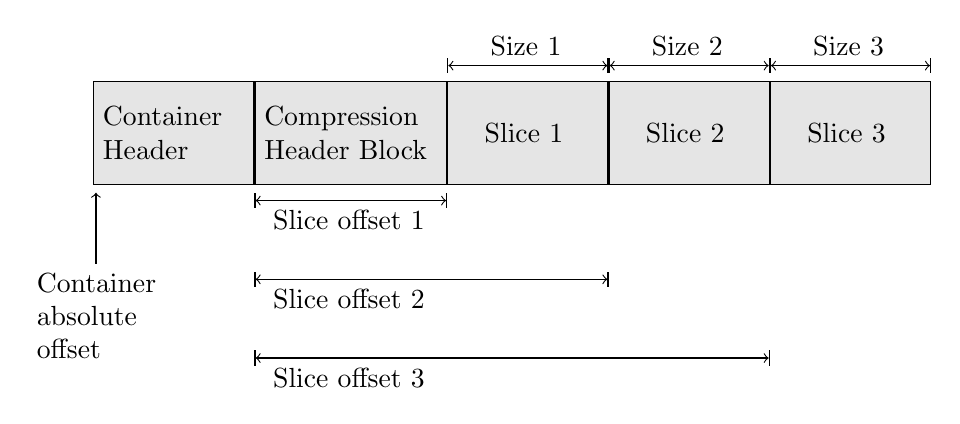
\begin{tikzpicture}[
  boxed/.style={rectangle, draw=black, fill=black!10, minimum height=1.3cm, text width=1.8cm},
]
\node(A) [boxed]{Container Header};
\node(B) [boxed,right,text width=2.2cm] at (A.east){Compression Header Block};
\node(C) [boxed,right] at (B.east){\quad Slice 1};
\node(D) [boxed,right] at (C.east){\quad Slice 2};
\node(E) [boxed,right] at (D.east){\quad Slice 3};

\draw[<-] (A.south west)+(1pt,-0.1cm) -- +(1pt,-1cm)
     node[below, text width=1.5cm]{Container absolute offset};


\draw[|<->|] ([yshift=-0.2cm]B.south west) node[below,xshift=1.2cm]{Slice offset 1}
    -- ([yshift=-0.2cm]B.south east);
\draw[|<->|] ([yshift=-1.2cm]B.south west) node[below,xshift=1.2cm]{Slice offset 2}
    -- ([yshift=-1.2cm]C.south east);
\draw[|<->|] ([yshift=-2.2cm]B.south west) node[below,xshift=1.2cm]{Slice offset 3}
    -- ([yshift=-2.2cm]D.south east);

\draw[|<->|] ([yshift=+0.2cm]C.north west) node[above,xshift=1cm]{Size 1} -- ([yshift=+0.2cm]C.north east);
\draw[|<->|] ([yshift=+0.2cm]D.north west) node[above,xshift=1cm]{Size 2} -- ([yshift=+0.2cm]D.north east);
\draw[|<->|] ([yshift=+0.2cm]E.north west) node[above,xshift=1cm]{Size 3} -- ([yshift=+0.2cm]E.north east);


\end{tikzpicture}
\end{center}

\subsubsection*{BAM index}

BAM indexes are supported by using 4-byte integer pointers called landmarks that 
are stored in container header. BAM index pointer is a 64-bit value with 48 bits 
reserved for the BAM block start position and 16 bits reserved for the in-block 
offset. When used to index CRAM files, the first 48 bits are used to store the 
CRAM container start position and the last 16 bits are used to store the index 
of the landmark in the landmark array stored in  container header. The landmark 
index can be used to access the appropriate slice. 

The above indexing scheme treats CRAM slices as individual records in BAM file. 
This allows to apply BAM indexing to CRAM files, however it introduces some overhead 
in seeking specific alignment start because all preceding records in the slice 
must be read and discarded.

\section{\textbf{Encodings}}
\label{sec:encodings}

% FIXME: we have a mishash of coding, encoding and codec.  We should
% go through the entire document and be consistent.

\subsection{\textbf{Introduction}}

The basic idea for codings is to efficiently represent some values in binary format. 
This can be achieved in a number of ways that most frequently involve some knowledge 
about the nature of the values being encoded, for example, distribution statistics. 
The methods for choosing the best encoding and determining its parameters are very 
diverse and are not part of the CRAM format specification, which only describes 
how the information needed to decode the values should be stored.

Note two of the encodings (Golomb and Golomb-Rice) are listed as deprecated.
These are still formally part of the CRAM specification, but have not been used by the primary implementations and may not be well supported.
Therefore their use is permitted, but not recommended.

\subsubsection*{Offset}

Many of the codings listed below encode positive integer numbers. An integer offset 
value is used to allow any integer numbers and not just positive ones to be encoded. 
It can also be used for monotonically decreasing distributions with the maximum 
not equal to zero. For example, given offset is 10 and the value to be encoded 
is 1, the actually encoded value would be offset+value=11. Then when decoding, 
the offset would be subtracted from the decoded value. 

\subsection{EXTERNAL: codec ID 1}

Can encode types \textit{Byte}, \textit{Integer}.

The EXTERNAL coding is simply storage of data verbatim to an external block with a given ID.
If the type is \textit{Byte} the data is stored as-is, otherwise for \textit{Integer} type the data is stored in ITF8.

\subsubsection*{Parameters}

CRAM format defines the following parameters of EXTERNAL coding: 

\begin{tabular}{|>{\raggedright}p{100pt}|>{\raggedright}p{100pt}|>{\raggedright}p{230pt}|}
\hline
\textbf{Data type} & \textbf{Name} & \textbf{Comment}
\tabularnewline
\hline
itf8 & external id & id of an external block containing the byte stream\tabularnewline
\hline
\end{tabular}

\subsection{Huffman coding: codec ID 3}

Can encode types \textit{Byte}, \textit{Integer}.

Huffman coding replaces symbols (values to encode) by binary codewords, with common symbols having shorter codewords such that the total message of binary codewords is shorter than using uniform binary codeword lengths.
The general process consists of the following steps.

\begin{itemize}
\item Obtain symbol code lengths.
\begin{itemize}
\item If encoding:\\
- Compute symbol frequencies.\\
- Compute code lengths from frequencies.
\item If decoding:\\
- Read code lengths from codec parameters.
\end{itemize}

\item Compute canonical Huffman codewords from code lengths\footnote{\url{https://en.wikipedia.org/wiki/Canonical_Huffman_code}}.

\item Encode or decode bits as per the symbol to codeword table.
Codewords have the ``prefix property'' that no codeword is a prefix of another codeword, enabling unambiguous decode bit by bit.
\end{itemize}

The use of canonical Huffman codes means that we only need to store the code lengths and use the same algorithm in both encoder and decoder to generate the codewords.
This is achieved by ensuring our symbol alphabet has a natural sort order and codewords are assigned in numerical order.

\textbf{Important note: for alphabets with only one value, the codeword will be zero bits long.}
This makes the Huffman codec an efficient mechanism for specifying constant values.

\subsubsection*{Canonical code computation}

\begin{enumerate}
\item Sort the alphabet ascending using bit-lengths and then using numerical order 
of the values.

\item The first symbol in the list gets assigned a codeword which is the same length 
as the symbol's original codeword but all zeros. This will often be a single zero 
('0').

\item Each subsequent symbol is assigned the next binary number in sequence, ensuring
that following codes are always higher in value.

\item When you reach a longer codeword, then after incrementing, append zeros until 
the length of the new codeword is equal to the length of the old codeword.
\end{enumerate}

\subsubsection*{Examples}

\begin{tabular}{|>{\raggedright}p{105pt}|>{\raggedright}p{105pt}|>{\raggedright}p{105pt}|}
\hline
\textbf{Symbol} & \textbf{Code length} & \textbf{Codeword}\tabularnewline
\hline
A & 1 & 0\tabularnewline
\hline
B & 3 & 100\tabularnewline
C & 3 & 101\tabularnewline
D & 3 & 110\tabularnewline
\hline
E & 4 & 1110\tabularnewline
F & 4 & 1111\tabularnewline
\hline
\end{tabular}

\subsubsection*{Parameters}

\begin{tabular}{|>{\raggedright}p{100pt}|>{\raggedright}p{100pt}|>{\raggedright}p{230pt}|}
\hline
\textbf{Data type} & \textbf{Name} & \textbf{Comment}
\tabularnewline
\hline
itf8[ ] & alphabet & list of all encoded symbols (values)\tabularnewline
\hline
itf8[ ] & bit-lengths & array of bit-lengths for each symbol in the alphabet\tabularnewline
\hline
\end{tabular}

\subsection{Byte array coding}

Often there is a need to encode an array of bytes where the length is not predetermined.
For example the read identifiers differ per alignment record, possibly with different lengths, and this length must be stored somewhere.
There are two choices available: storing the length explicitly (BYTE\_ARRAY\_LEN) or continuing to read bytes until a termination value is seen (BYTE\_ARRAY\_STOP).

Note in contrast to this, quality values are known to be the same length as the sequence which is an already known quantity, so this does not need to be encoded using the byte array codecs.

\subsubsection*{BYTE\_ARRAY\_LEN: codec ID 4}

Can encode types \textit{Byte[ ]}.

Byte arrays are captured length-first, meaning that the length of every array element is written using an additional encoding.
For example this could be a HUFFMAN encoding or another EXTERNAL block.
The length is decoded first followed by the data, followed by the next length and data, and so on.

This encoding can therefore be considered as a nested encoding, with each pair of nested encodings containing their own set of parameters.
The byte stream for parameters of the BYTE\_ARRAY\_LEN encoding is therefore the concatenation of the length and value encoding parameters as described in section~\ref{subsec:writing-bytes}.

The parameter for BYTE\_ARRAY\_LEN are listed below:

\begin{tabular}{|>{\raggedright}p{100pt}|>{\raggedright}p{100pt}|>{\raggedright}p{230pt}|}
\hline
\textbf{Data type} & \textbf{Name} & \textbf{Comment}
\tabularnewline
\hline
encoding\texttt{<}int\texttt{>} & lengths encoding & an encoding describing how 
the arrays lengths are captured\tabularnewline
\hline
encoding\texttt{<}byte\texttt{>} & values encoding & an encoding describing how 
the values are captured\tabularnewline
\hline
\end{tabular}

For example, the bytes specifying a BYTE\_ARRAY\_LEN encoding, including the codec and parameters, for a 16-bit X0 auxiliary tag (``X0C'') may use HUFFMAN encoding to specify the length (always 2 bytes) and an EXTERNAL encoding to store the value to an external block with ID 200.

\begin{tabular}{lll}
\hline
\textbf{Bytes} & & \textbf{Meaning}\\
\hline
\texttt{0x04}         & & BYTE\_ARRAY\_LEN codec ID                                    \\
\texttt{0x0a}         & & 10 remaining bytes of BYTE\_ARRAY\_LEN parameters            \\
\\
\texttt{0x03}         & & HUFFMAN codec ID, for aux tag lengths                        \\
\texttt{0x04}         & & 4 more bytes of HUFFMAN parameters                           \\
\texttt{0x01}         & & Alphabet array size = 1                                      \\
\texttt{0x02}         & & alphabet symbol; (length = 2)                                \\
\texttt{0x01}         & & Codeword array size = 1                                      \\
\texttt{0x00}         & & Code length = 0 (zero bits needed as alphabet is size 1)     \\
\\
\texttt{0x01}         & & EXTERNAL codec ID, for aux tag values                        \\
\texttt{0x02}         & & 2 more bytes of EXTERNAL parameters                          \\
\texttt{0x80 0xc8}    & & ITF8 encoding for block ID 200                               \\
\hline
\end{tabular}



\subsubsection*{BYTE\_ARRAY\_STOP: codec ID 5}

Can encode types \textit{Byte[ ]}.

Byte arrays are captured as a sequence of bytes terminated by a special stop byte.
The data returned does not include the stop byte itself.
In contrast to BYTE\_ARRAY\_LEN the value is always encoded with EXTERNAL so the parameter is an external id instead of another encoding.

\begin{tabular}{|>{\raggedright}p{100pt}|>{\raggedright}p{100pt}|>{\raggedright}p{230pt}|}
\hline
\textbf{Data type} & \textbf{Name} & \textbf{Comment}
\tabularnewline
\hline
byte & stop byte & a special byte treated as a delimiter\tabularnewline
\hline
itf8 & external id & id of an external block containing the byte stream\tabularnewline
\hline
\end{tabular}

\subsection{Beta coding: codec ID 6}

Can encode types \textit{Integer}.

\subsubsection*{Definition}

Beta coding is a most common way to represent numbers in \emph{binary notation} and is sometimes referred to as binary coding.
The decoder reads the specified fixed number of bits (most significant first) and subtracts the offset value to get the decoded integer.

\subsubsection*{Parameters}

CRAM format defines the following parameters of beta coding: 

\begin{tabular}{|>{\raggedright}p{144pt}|>{\raggedright}p{144pt}|>{\raggedright}p{144pt}|}
\hline
\textbf{Data type} & \textbf{Name} & \textbf{Comment}\tabularnewline
\hline
itf8 & offset & offset is subtracted from each value during decode\tabularnewline
\hline
itf8 & length & the number of bits used\tabularnewline
\hline
\end{tabular}

\subsubsection*{Examples}

If we have integer values in the range 10 to 15 inclusive, the largest value would traditionally need 4 bits, but with an offset of -10 we can hold values 0 to 5, using a fixed size of 3 bits.
Using fixed Offset and Length coming from the beta parameters, we decode these values as:

\begin{tabular}{|>{\raggedright}p{105pt}|>{\raggedright}p{105pt}|>{\raggedright}p{105pt}|>{\raggedright}p{105pt}|}
\hline
Offset & Length & \textbf{Bits} & \textbf{Value}\tabularnewline
\hline
-10 & 3 & 000 & 10\tabularnewline
\hline
-10 & 3 & 001 & 11\tabularnewline
\hline
-10 & 3 & 010 & 12\tabularnewline
\hline
-10 & 3 & 011 & 13\tabularnewline
\hline
-10 & 3 & 100 & 14\tabularnewline
\hline
-10 & 3 & 101 & 15\tabularnewline
\hline
\end{tabular}

\subsection{Subexponential coding: codec ID 7}

Can encode types \textit{Integer}.

\subsubsection*{Definition}

Subexponential coding\footnote{Fast progressive lossless image compression, Paul G. Howard and Jeffrey Scott Vitter, 1994. \url{http://www.ittc.ku.edu/~jsv/Papers/HoV94.progressive_FELICS.pdf}} is parametrized by a non-negative integer $k$.
For values $n < 2^{k+1}$ subexponential coding produces codewords identical to Rice coding \footnote{\url{https://en.wikipedia.org/wiki/Golomb_coding\#Rice_coding}}.  For larger values it grows logarithmically with $n$.

\subsubsection*{Encoding}

\begin{enumerate}
\item Add $\mathit{offset}$ to $n$.

\item Determine $u$ and $b$ values from $n$
\begin{align*}
b =
\begin{cases}
  \ k                        & \text{ if $n < 2^k$} \\
  \ \lfloor log_{2}n \rfloor & \text{ if $n \ge 2^k$}
\end{cases}
&\
&u =
\begin{cases}
  \ 0     & \text{ if $n < 2^k$} \\
  \ b-k+1 & \text{ if $n \ge 2^k$}
\end{cases}
\end{align*}

\item Write $u$ in unary form; $u$ 1 bits followed by a single 0 bit.

\item Write the bottom $b$-bits of $n$ in binary form.
\end{enumerate}

\subsubsection*{Decoding}

\begin{enumerate}
\item Read $u$ in unary form, counting the number of leading 1s (prefix) in the codeword (discard the trailing 0 bit).

\item Determine $n$ via:
\begin{enumerate}
\item if $u = 0$ then read $n$ as a $k$-bit binary number.
\item if $u \ge 1$ then read $x$ as a $(u + k - 1)$-bit binary. Let $n = 2^{u+k-1} + x$.
\end{enumerate}

\item Subtract $\mathit{offset}$ from $n$.
\end{enumerate}

\subsubsection*{Examples}

\begin{tabular}{|>{\raggedright}p{105pt}|>{\raggedright}p{105pt}|>{\raggedright}p{105pt}|>{\raggedright}p{105pt}|}
\hline
\textbf{Number} & \textbf{Codeword, k=0} & \textbf{Codeword, k=1} & \textbf{Codeword, 
k=2}\tabularnewline
\hline
0 & 0 & 00 & 000\tabularnewline
\hline
1 & 10 & 01 & 001\tabularnewline
\hline
2 & 1100 & 100 & 010\tabularnewline
\hline
3 & 1101 & 101 & 011\tabularnewline
\hline
4 & 111000 & 11000 & 1000\tabularnewline
\hline
5 & 111001 & 11001 & 1001\tabularnewline
\hline
6 & 111010 & 11010 & 1010\tabularnewline
\hline
7 & 111011 & 11011 & 1011\tabularnewline
\hline
8 & 11110000 & 1110000 & 110000\tabularnewline
\hline
9 & 11110001 & 1110001 & 110001\tabularnewline
\hline
10 & 11110010 & 1110010 & 110010\tabularnewline
\hline
\end{tabular}

\subsubsection*{Parameters}

\begin{tabular}{|>{\raggedright}p{100pt}|>{\raggedright}p{100pt}|>{\raggedright}p{230pt}|}
\hline
\textbf{Data type} & \textbf{Name} & \textbf{Comment}
\tabularnewline
\hline
itf8 & offset & offset is subtracted from each value during decode\tabularnewline
\hline
itf8 & k & the order of the subexponential coding\tabularnewline
\hline
\end{tabular}

\subsection{Gamma coding: codec ID 9}

Can encode types \textit{Integer}.

\subsubsection*{Definition}

\emph{Elias gamma code} is a prefix encoding of positive integers. This is a combination 
of unary coding and beta coding. The first is used to capture the number of bits 
required for beta coding to capture the value. 

\subsubsection*{Encoding}

\begin{enumerate}
\item Write it in binary.

\item Subtract $1$ from the number of bits written in step 1 and prepend that many zeros.

\item An equivalent way to express the same process:

\item Separate the integer into the highest power of $2$ it contains ($2N$) and the remaining 
$N$ binary digits of the integer.

\item Encode $N$ in unary; that is, as $N$ zeroes followed by a one.

\item Append the remaining $N$ binary digits to this representation of $N$.
\end{enumerate}

\subsubsection*{Decoding}

\begin{enumerate}
\item Read and count 0s from the stream until you reach the first 1. Call this count 
of zeroes $N$.

\item Considering the one that was reached to be the first digit of the integer, with 
a value of $2N$, read the remaining $N$ digits of the integer.
\end{enumerate}

\subsubsection*{Examples}

\begin{tabular}{|>{\raggedright}p{76pt}|>{\raggedright}p{107pt}|}
\hline
\textbf{Value} & \textbf{Codeword}\tabularnewline
\hline
1 & 1\tabularnewline
\hline
2 & 010\tabularnewline
\hline
3 & 011\tabularnewline
\hline
4 & 00100\tabularnewline
\hline
\end{tabular}

\subsubsection*{Parameters}

\begin{tabular}{|>{\raggedright}p{144pt}|>{\raggedright}p{144pt}|>{\raggedright}p{144pt}|}
\hline
\textbf{Data type} & \textbf{Name} & \textbf{Comment}\tabularnewline
\hline
itf8 & offset & offset to subtract from each value after decode\tabularnewline
\hline
\end{tabular}

\subsection{DEPRECATED: Golomb coding: codec ID 2}

Can encode types \textit{Integer}.

Note this codec has not been used in any known CRAM implementation since before CRAM v1.0.
Nor is it implemented in some of the major software.
Therefore its use is not recommended.

\subsubsection*{Definition}

\emph{Golomb encoding} is a prefix encoding optimal for representation of random 
positive numbers following geometric distribution. 

\subsubsection*{Encoding}

\begin{enumerate}
\item Fix the parameter $M$ to an integer value.

\item For $N$, the number to be encoded, find

\begin{enumerate}
\item quotient $q = \lfloor N/M \rfloor$

\item remainder $r = N \bmod M$
\end{enumerate}

\item Generate Codeword

\begin{enumerate}
\item The Code format : \texttt{<}Quotient Code\texttt{>}\texttt{<}Remainder Code\texttt{>}, 
where

\item Quotient Code (in unary coding)

\begin{enumerate}
\item Write a $q$-length string of 1 bits

\item Write a 0 bit
\end{enumerate}

\item Remainder Code (in truncated binary encoding)

Set $b=\lceil log_{2}(M) \rceil$

\begin{enumerate}
\item If $r < 2^{b}-M$ code $r$ as plain binary using $b-1$ bits.

\item If $r \ge 2^{b}-M$ code the number $r+2^{b}-M$ in plain binary representation 
using $b$ bits.
\end{enumerate}
\end{enumerate}
\end{enumerate}

\subsubsection*{Decoding}

\begin{enumerate}
\item Read $q$ via unary coding: count the number of 1 bits and consume the following 0 bits.
\item Set $b=\lceil log_{2}(M) \rceil$
\item Read $r$ via $b-1$ bits of binary coding
\item If $r \ge 2^{b}-M$
\begin{enumerate}
\item Read 1 single bit, $x$.
\item Set $r = r*2 + x - (2^{b}-M)$
\end{enumerate}
\item Value is $q*M + r - \mathit{offset}$
\end{enumerate}

\subsubsection*{Examples}

\begin{tabular}{|>{\raggedright}p{76pt}|>{\raggedright}p{107pt}|}
\hline
\textbf{Number} & \textbf{Codeword, M=10, (thus b=4)}\tabularnewline
\hline
0 & 0000\tabularnewline
\hline
4 & 0100\tabularnewline
\hline
10 & 10000\tabularnewline
\hline
26 & 1101100\tabularnewline
\hline
42 & 11110010\tabularnewline
\hline
\end{tabular}

\subsubsection*{Parameters}

Golomb coding takes the following parameters: 

\begin{tabular}{|>{\raggedright}p{144pt}|>{\raggedright}p{144pt}|>{\raggedright}p{144pt}|}
\hline
\textbf{Data type} & \textbf{Name} & \textbf{Comment}\tabularnewline
\hline
itf8 & offset & offset is added to each value\tabularnewline
\hline
itf8 & M & the golomb parameter (number of bins)\tabularnewline
\hline
\end{tabular}

\subsection{DEPRECATED: Golomb-Rice coding: codec ID 8}

Can encode types \textit{Integer}.

Note this codec has not been used in any known CRAM implementation since before CRAM v1.0.
Nor is it implemented in some of the major software.
Therefore its use is not recommended.

Golomb-Rice coding is a special case of Golomb coding when the M parameter is a power of 2.
The reason for this coding is that the division operations in Golomb coding can be replaced with bit shift operators as well as avoiding the extra $r < 2^{b}-M$ check.

\section{\textbf{External compression methods}}

External encoding operates on bytes only. Therefore any data series must be translated into bytes before sending data into an external block.
The following methods are defined.
Exact definitions of these methods are in their respective internet links or the ancillary \textit{CRAMcodecs} document found along side this specification.

Integer values are written as ITF8, which then can be translated into an array 
of bytes. 

Strings, like read name, are translated into bytes according to UTF8 rules. In 
most cases these should coincide with ASCII, making the translation trivial.

Each method has an associated numeric code which is defined in Section~\ref{sec:block-struct}.

\subsection{\textbf{Gzip}}

The Gzip specification is defined in RFC 1952.
Gzip in turn is an encapsulation on the Deflate algorithm defined in RFC 1951.

\subsection{\textbf{Bzip2}}

First available in CRAM v2.0.

Bzip2 is a compression method utilising the Burrows Wheeler Transform, Move To Front transform, Run Length Encoding and a Huffman entropy encoder. 
It is often superior to Gzip for textual data.

An informal format specification exists:\\
\url{https://github.com/dsnet/compress/blob/master/doc/bzip2-format.pdf}

\subsection{\textbf{LZMA}}

First available in CRAM v3.0.

LZMA is the Lempel-Ziv Markov chain algorithm.
CRAM uses the xz Stream format to encapsulate this algorithm, as defined in \url{https://tukaani.org/xz/xz-file-format.txt}.

\subsection{\textbf{rANS4x8 codec}}

First available in CRAM v3.0.

rANS is the range-coder variant of the Asymmetric Numerical
System\footnote{J. Duda, \textit{Asymmetric numeral systems: entropy
    coding combining speed of Huffman coding with compression rate of
    arithmetic coding}, \url{http://arxiv.org/abs/1311.2540}}.

``4x8'' refers to 4-way interleaving with 8-bit renormalisation.\newline
This variant of rANS first appeared in CRAM v3.0.

Details of this algorithm have been moved to the \textit{CRAMcodecs} document.

\subsection{\textbf{rANS4x16 codec}}

First available in CRAM v3.1.

``4x16'' refers to 4-way interleaving with 16-bit renormalisation.\newline
This variant of rANS first appeared in CRAM v3.1.

Details of this algorithm are listed in the \textit{CRAMcodecs} document.

\subsection{\textbf{adaptive arithemtic coding}}

First available in CRAM v3.1.

An entropy encoder that is slower but slightly more concise than
rANS.  It achieves this by adapting the probabilities as it compresses
and decompresses instead of using a fixed table.

Details of this algorithm are listed in the \textit{CRAMcodecs} document.

\subsection{\textbf{fqzcomp codec}}

First available in CRAM v3.1.

This is a method dedicated to compression of quality values.

Details of this algorithm are listed in the \textit{CRAMcodecs} document.

\subsection{\textbf{name tokeniser}}

First available in CRAM v3.1.

This is a method dedicated to compression of read names.

Details of this algorithm are listed in the \textit{CRAMcodecs} document.

\section{\textbf{Appendix}}
\subsection{\textbf{Choosing the container size}}

CRAM format does not constrain the size of the containers. However, the following 
should be considered when deciding the container size:

$\bullet$ Data can be compressed better by using larger containers

$\bullet$ Random access performance is better for smaller containers 

$\bullet$ Streaming is more convenient for small containers

$\bullet$ Applications typically buffer containers into memory

We recommend 1 megabyte containers. They are small enough to provide good random access
and streaming performance while being large enough to provide good compression. 
1\MB\ containers are also small enough to fit into the L2 cache of most modern CPUs.

Some simplified examples are provided below to fit data into 1\MB\ containers.

\textbf{Unmapped short reads with bases, read names, recalibrated and original 
quality scores}

We have 10,000 unmapped short reads (100bp) with read names, recalibrated and original 
quality scores. We estimate 0.4 bits/base (read names) + 0.4 bits/base (bases) 
+ 3 bits/base (recalibrated quality scores) + 3 bits/base (original quality scores) 
$\approx$ 7 bits/base. Space estimate is $10\,000 \times 100 \times 7 \bits
\approx 0.9 \MB$. Data could be stored in a single container.

\textbf{Unmapped long reads with bases, read names and quality scores}

We have 10,000 unmapped long reads (10kb) with read names and quality scores. We 
estimate: 0.4 bits/base (bases) + 3 bits/base (original quality scores) $\approx$
3.5 bits/base. Space estimate is $10\,000 \times 10\,000 \times 3.5 \bits
\approx 42 \MB$. Data could be stored in $42 \times 1\MB$ containers.

\textbf{Mapped short reads with bases, pairing and mapping information}

We have 250,000 mapped short reads (100bp) with bases, pairing and mapping information. 
We estimate the compression to be 0.2 bits/base. Space estimate is $250\,000 \times 100
\times 0.2 \bits \approx 0.6 \MB$. Data could be stored in a single
container.

\textbf{Embedded reference sequences}

We have a reference sequence (10Mb). We estimate the compression to be 2 bits/base. 
Space estimate is $10\,000\,000 \times 2 \bits \approx 2.4 \MB$. Data
could be written into three containers: $1\MB + 1\MB + 0.4\MB$.

\newpage

\subsection{CRAM History}

\subsubsection*{Pre-CRAM: 2010}

The primary concepts and ideas of CRAM stem from work at the European
Bioinformatics Institute in 2010 and 2011, published in:

\begin{quote}\small
Markus Hsi-Yang Fritz,
Rasko Leinonen, Guy Cochrane, and Ewan Birney,
\textbf{Efficient storage of high throughput DNA sequencing data using reference-based compression},
{\sl Genome Res.}~2011~21: 734--740;
\href{http://dx.doi.org/doi:10.1101/gr.114819.110}{doi:10.1101/gr.114819.110};
{\sc pmid:}21245279.
\end{quote}

\subsubsection*{CRAM 0.x: 2011}

Vadim Zalunin implemented the ideas in the paper, now named CRAM, in
the Java CRAMtools package.  This included versions from 0.3 to 0.86\footnote{\url{https://github.com/vadimzalunin/crammer/releases}}.

\subsubsection*{CRAM 1.0: 2012}

The first official launch of the CRAM specification, in the Java
CRAMtools package\footnote{\url{https://github.com/enasequence/cramtools}}

This was publicised at \url{https://github.com/enasequence/cramtools}.

\subsubsection*{CRAM 2.0: 2013}

Reimplementing CRAM in C
\footnote{Staden IO\_Lib 1.13.0 and later HTSlib 0.2.0} exposed a number of issues with the
1.0 specification and disparities between the specification text and
the Java implementation.  CRAM 2.0 unified implementation with
specification.

Other changes included:

\begin{itemize}
\item Support for multiple references per container, to permit storage
of highly fragmented assemblies.

\item Soft-clips and inserted bases moved to their own separate
data-series instead of sharing one.

\item Slice headers contain meta-data tracking the number of records
and bases.

\item Corrected the BF (bam flag) data series to match the BAM
specification.

\item Improved encoding of auxiliary tags.
\end{itemize}

\subsubsection*{CRAM 2.1: 2014}

This is the first version to appear in HTSJDK (version 1.127), ported
from the Java CRAMtools package.

\begin{itemize}
\item EOF blocks are added in order to spot truncated files.
\end{itemize}

\subsubsection*{CRAM 3.0: 2014}

Primarily this is an optimisation of size and speed.

\begin{itemize}
\item Inclusion of LZMA compression library.
\item Inclusion of the custom rANS Order-0 and Order-1 entropy encoders.
\item Checksums added to all file format structures to ensure data integrity.
\end{itemize}

\subsubsection*{CRAM 3.1: 2023}

Note: the formal draft appeared in 2019, and was initially
demonstrated in 2016.

This adds new EXTERNAL compression methods, described in the separate
CRAMcodecs document, and expands the list of permitted ``methods'' in
the CRAM Block structure.

The aim of the new compression methods is improved compression, both
performance with the newer SIMD rANS implementation and file size with
custom name tokeniser and quality codec.

The format is otherwise identical to 3.0.

\newpage

\subsection{\textbf{Contributors and Acknowledgements}}

\begin{itemize}
\item
Markus Fritz, Rasko Leinonen, Guy Cochrane and Ewan Birney (EBI):
Initial ideas behind CRAM.

\item Vadim Zalunin (EBI):
Initial JAVA implementation of CRAM and previous maintainer of CRAM specification.

\item James Bonfield (Sanger Institute):
Initial C implementation of CRAM and current maintainer of CRAM
specification.

\item Joel Thibault (Broad Institute):
previous maintainer of CRAM specification.

\item Chris Norman (Broad Institute):
previous maintainer of CRAM specification and worked on
the HTSJDK implementation.

\item Robert Buels (UC Berkeley): First JavaScript implementation of CRAM

\item Michael Macias (St Jude Children's Research Hospital): First Rust implementation of CRAM

\item Other specification contributors include: John Marshall, Rishi Nag,
Kenta Sato, Artem Tarasov and Jason Travis.

\item Plus a big thank you to everyone who has raised GitHub issues
and/or helped us improve the specification in other ways.
\end{itemize}

\end{document}

\title{CRAM format specification (version 3.1)}
\author{samtools-devel@lists.sourceforge.net}
\date{\headdate}
\maketitle


\begin{quote}\small
The master version of this document can be found at
\url{https://github.com/samtools/hts-specs}.\\
This printing is version~\commitdesc\ from that repository,
last modified on the date shown above.
\end{quote}

\begin{center}
\textit{license: Apache 2.0}
\end{center}
\vspace*{1em}

\section{\textbf{Overview}}

This specification describes the CRAM 3.0 and 3.1 formats.

CRAM has the following major objectives:

\begin{enumerate}
\item Significantly better lossless compression than BAM

\item Full compatibility with BAM

\item Effortless transition to CRAM from using BAM files

\item Support for controlled loss of BAM data
\end{enumerate}

The first three objectives allow users to take immediate advantage of the CRAM 
format while offering a smooth transition path from using BAM files. The fourth 
objective supports the exploration of different lossy compression strategies and 
provides a framework in which to effect these choices. Please note that the CRAM 
format does not impose any rules about what data should or should not be preserved. 
Instead, CRAM supports a wide range of lossless and lossy data preservation strategies 
enabling users to choose which data should be preserved.

Data in CRAM is stored either as CRAM records or using one of the general purpose 
compressors (gzip, bzip2). CRAM records are compressed using a number of different 
encoding strategies. For example, bases are reference compressed by encoding base
differences rather than storing the bases themselves.\footnote{Markus Hsi-Yang Fritz,
Rasko Leinonen, Guy Cochrane, and Ewan Birney,
\textbf{Efficient storage of high throughput DNA sequencing data using reference-based compression},
{\sl Genome Res.}~2011~21: 734--740;
\href{http://dx.doi.org/doi:10.1101/gr.114819.110}{doi:10.1101/gr.114819.110};
{\sc pmid:}21245279.}

\section{\textbf{Data types}}

CRAM specification uses logical data types and storage data types; logical data 
types are written as words (e.g. int) while physical data types are written using 
single letters (e.g. i). The difference between the two is that storage data types 
define how logical data types are stored in CRAM. Data in CRAM is stored either 
as bits or bytes. Writing values as bits and bytes is described in detail 
below.

\subsection{\textbf{Logical data types}}

\begin{description}
\item[Byte]\ \newline
Signed byte (8 bits).

\item[Integer]\ \newline
Signed 32-bit integer. 

\item[Long]\ \newline
Signed 64-bit integer. 

\item[Array]\ \newline
An array of any logical data type: array\texttt{<}type\texttt{>}
\end{description}

% \begin{tabular}{ll}
% \textbf{Byte}    & Signed byte (8 bits).  \\
% \\
% \textbf{Integer} & Signed 32-bit integer. \\
% \\
% \textbf{Long}    & Signed 64-bit integer. \\
% \\
% \textbf{Array}   & An array of any logical data type: \texttt{<}type\texttt{>}[ ] \\
% \end{tabular}

\subsection{\textbf{Writing bits to a bit stream}}

A bit stream consists of a sequence of 1s and 0s. The bits are written most significant 
bit first where new bits are stacked to the right and full bytes on the left are 
written out. In a bit stream the last byte will be incomplete if less than 8 bits 
have been written to it. In this case the bits in the last byte are shifted to 
the left.

\subsubsection*{Example of writing to bit stream}

Let's consider the following example. The table below shows a sequence of write 
operations: 

\begin{tabular}{|l|l|l|l|l|}
\hline
\textbf{Operation order} & \textbf{Buffer state before} & \textbf{Written bits} & \textbf{Buffer state after} & \textbf{Issued bytes}\tabularnewline
\hline
1 & 0x0 & 1 & 0x1 & -\tabularnewline
\hline
2 & 0x1 & 0 & 0x2 & -\tabularnewline
\hline
3 & 0x2 & 11 & 0xB & -\tabularnewline
\hline
4 & 0xB & 0000 0111 & 0x7 & 0xB0\tabularnewline
\hline
\end{tabular}

After flushing the above bit stream the following bytes are written: 0xB0 0x70. 
Please note that the last byte was 0x7 before shifting to the left and became 0x70 
after that:

\texttt{> echo "obase=16; ibase=2; 00000111" \textbar{} bc\\
7\\
\\
> echo "obase=16; ibase=2; 01110000" \textbar{} bc\\
70}

And the whole bit sequence: 

\texttt{> echo "obase=2; ibase=16; B070" \textbar{} bc\\
1011000001110000}

When reading the bits from the bit sequence it must be known that only 12 bits 
are meaningful and the bit stream should not be read after that. 

\subsubsection*{Note on writing to bit stream}

When writing to a bit stream both the value and the number of bits in the value 
must be known. This is because programming languages normally operate with bytes 
(8 bits) and to specify which bits are to be written requires a bit-holder, for 
example an integer, and the number of bits in it. Equally, when reading a value 
from a bit stream the number of bits must be known in advance. In case of prefix 
codes (e.g. Huffman) all possible bit combinations are either known in advance 
or it is possible to calculate how many bits will follow based on the first few 
bits. Alternatively, two codes can be combined, where the first contains the number 
of bits to read. 

\subsection{\textbf{Writing bytes to a byte stream}}
\label{subsec:writing-bytes}

The interpretation of byte stream is straightforward. CRAM uses \emph{little endianness}
for bytes when applicable and defines the following storage data types:

\begin{description}

\item[Boolean (bool)]\ \newline
Boolean is written as 1-byte with 0x0 being `false' and 0x1 being `true'.

\item[Integer (int32)]\ \newline
Signed 32-bit integer, written as 4 bytes in little-endian byte order.

\item[Long (int64)]\ \newline
Signed 64-bit integer, written as 8 bytes in little-endian byte order.

\item[ITF-8 integer (itf8)]\ \newline
This is an alternative way to write an integer value. The idea is similar to UTF-8 
encoding and therefore this encoding is called ITF-8 (Integer Transformation Format 
- 8 bit). 

The most significant bits of the first byte have special meaning and are called 
`prefix'. These are 0 to 4 true bits followed by a 0. The number of 1's denote 
the number of bytes to follow. To accommodate 32 bits such representation requires 
5 bytes with only 4 lower bits used in the last byte 5.

\item[LTF-8 long (ltf8)]\ \newline
See ITF-8 for more details. The only difference between ITF-8 and LTF-8 is the 
number of bytes used to encode a single value. To do so 64 bits are required and 
this can be done with 9 byte at most with the first byte consisting of just 1s 
or 0xFF value. 

\item[{Array (array\texttt{<}type\texttt{>})}]\ \newline
A variable sized array with an explicitly written dimension.
Array length is written first as integer (itf8), followed by the elements of the array.

Implicit or fixed-size arrays are also used, written as \textit{type}\texttt{[ ]} or \textit{type}\texttt{[4]} (for example).
These have no explicit dimension included in the file format and instead rely on the specification itself to document the array size.


\item[{Encoding}]\ \newline
Encoding is a data type that specifies how data series have been compressed. Encodings 
are defined as encoding\texttt{<}type\texttt{>} where the type is a logical data 
type as opposed to a storage data type.

An encoding is written as follows. The first integer (itf8) denotes the codec id 
and the second integer (itf8) the number of bytes in the following encoding-specific 
values. 

Subexponential encoding example: 

\begin{tabular}{|l|l|l|}
\hline
\textbf{Value} & \textbf{Type} & \textbf{Name}\tabularnewline
\hline
0x7 & itf8 & codec id\tabularnewline
\hline
0x2 & itf8 & number of bytes to follow\tabularnewline
\hline
0x0 & itf8 & offset\tabularnewline
\hline
0x1 & itf8 & K parameter\tabularnewline
\hline
\end{tabular}

The first byte ``0x7'' is the codec id. 

The next byte ``0x2'' denotes the length of the bytes to follow (2). 

The subexponential encoding has 2 parameters: integer (itf8) offset and integer (itf8) K.

offset = 0x0 = 0

K = 0x1 = 1


\item[{Map}]\ \newline
A map is a collection of keys and associated values. A map with N keys is written 
as follows: 

\begin{tabular}{|l|l|l|l|l|l|l|l|}
\hline
size in bytes & N & key 1 & value 1 & key ... & value ... & key N & value N\tabularnewline
\hline
\end{tabular}

Both the size in bytes and the number of keys are written as integer (itf8). Keys 
and values are written according to their data types and are specific to each map.

\item[String]\ \newline
A string is represented as byte arrays using UTF-8 format. Read names, reference 
sequence names and tag values with type `Z' are stored as UTF-8.

\end{description}


\section{\textbf{Encodings }}

Encoding is a data structure that captures information about compression details 
of a data series that are required to uncompress it. This could be a set of constants 
required to initialize a specific decompression algorithm or statistical properties 
of a data series or, in case of data series being stored in an external block, 
the block content id. 

Encoding notation is defined as the keyword `encoding' followed by its data type 
in angular brackets, for example `encoding\texttt{<}byte\texttt{>}' stands for 
an encoding that operates on a data series of data type `byte'. 

Encodings may have parameters of different data types, for example the EXTERNAL 
encoding has only one parameter, integer id of the external block. The following 
encodings are defined: 

\begin{tabular}{|l|l|>{\raggedright}p{155pt}|>{\raggedright}p{160pt}|}
\hline
\textbf{Codec} & \textbf{ID} & \textbf{Parameters} & \textbf{Comment}\tabularnewline
\hline
NULL & 0 & none & series not preserved\tabularnewline
\hline
EXTERNAL & 1 & int block content id & the block content identifier used to associate 
external data blocks with data series\tabularnewline
\hline
Deprecated (GOLOMB) & 2 & int offset, int M & Golomb coding\tabularnewline
\hline
HUFFMAN & 3 & array\texttt{<}int\texttt{>}, array\texttt{<}int\texttt{>} & coding with int/byte values\tabularnewline
\hline
BYTE\_ARRAY\_LEN & 4 & encoding\texttt{<}int\texttt{>} array length, encoding\texttt{<}byte\texttt{>} 
bytes & coding of byte arrays with array length\tabularnewline
\hline
BYTE\_ARRAY\_STOP & 5 & byte stop, int external block\linebreak{}
content id & coding of byte arrays with a stop value \tabularnewline
\hline
BETA & 6 & int offset, int number of bits & binary coding\tabularnewline
\hline
SUBEXP & 7 & int offset, int K & subexponential coding\tabularnewline
\hline
Deprecated (GOLOMB\_RICE) & 8 & int offset, int log$_{\text{2}}$m & Golomb-Rice coding\tabularnewline
\hline
GAMMA & 9 & int offset & Elias gamma coding\tabularnewline
\hline
\end{tabular}

See section~\ref{sec:encodings} for more detailed descriptions of all the above coding algorithms and their parameters.

\section{\textbf{Checksums}}
The checksumming is used to ensure data integrity. The following checksumming algorithms are used in CRAM.
\subsection{\textbf{CRC32}}
This is a cyclic redundancy checksum 32-bit long with the polynomial 0x04C11DB7. Please refer to \href{http://www.itu.int/rec/recommendation.asp?type=folders&lang=e&parent=T-REC-V.42}{ITU-T V.42} for more details. The value of the CRC32 hash function is written as an integer.
\subsection{\textbf{CRC32 sum}}
CRC32 sum is a combination of CRC32 values by summing up all individual CRC32 values modulo 2\textsuperscript{32}. 

\section{\textbf{File structure}}

The overall CRAM file structure is described in this section. Please refer to other 
sections of this document for more detailed information. 

A CRAM file consists of a fixed length file definition, followed by a CRAM header container,
then zero or more data containers, and finally a special end-of-file container.

\begin{center}
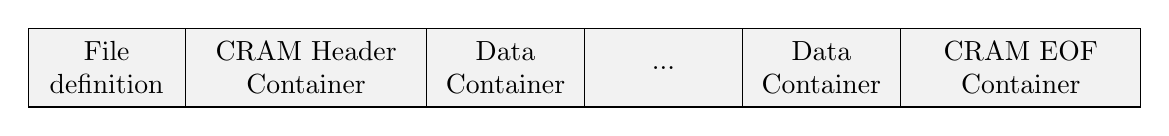
\begin{tikzpicture}[
  every node/.style={scale=1.0},
  boxes/.style={rectangle split,rectangle split parts=#1,draw,rectangle split horizontal,text width=5em,align=center,minimum height=1cm,fill=black!5,on grid},
  notes/.style={text width=20em,align=center,minimum height=1cm,on grid},
]
\node (file) [boxes=6] {
\nodepart{one}File definition
\nodepart[text width=8em]{two}CRAM Header Container
\nodepart{three}Data Container
\nodepart{four}...
\nodepart{five}Data Container
\nodepart[text width=8em]{six}CRAM EOF Container
};
\end{tikzpicture}

Figure 1: A CRAM file consists of a file definition, followed by a header container, then other containers.
\end{center}

Containers consist of one or more blocks. The first container, called the CRAM header container,
is used to store a textual header as described in the SAM specification (see the section 7.1).

\begin{center}
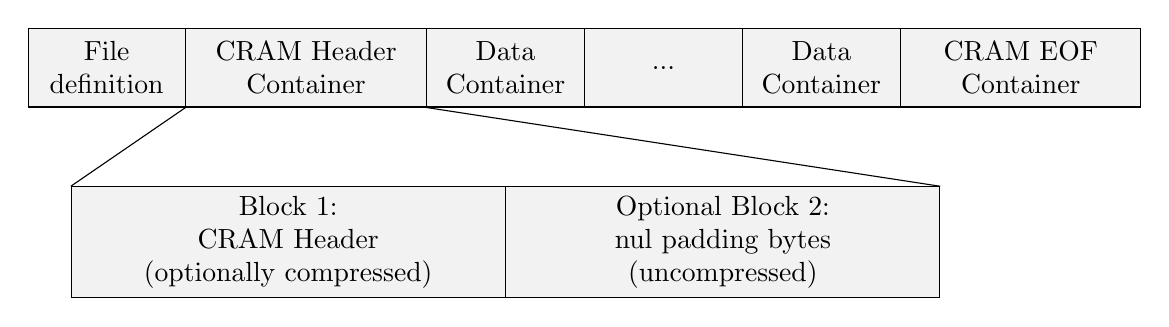
\begin{tikzpicture}[
  every node/.style={scale=1.0},
  boxes/.style={rectangle split,rectangle split parts=#1,draw,rectangle split horizontal,text width=5em,align=center,minimum height=1cm,fill=black!5,on grid},
  notes/.style={text width=20em,align=center,minimum height=1cm,on grid},
]
\node (file) [boxes=6] {
\nodepart{one}File definition
\nodepart[text width=8em]{two}CRAM Header Container
\nodepart{three}Data Container
\nodepart{four}...
\nodepart{five}Data Container
\nodepart[text width=8em]{six}CRAM EOF Container
};

\node (header) [boxes=2,below=1 of file.three south, text width=15em] {
\nodepart{one}Block 1:\break
CRAM Header\break
(optionally compressed)
\nodepart{two}Optional Block 2:\break
nul padding bytes\break
(uncompressed)
};
\draw (file.one split south) to (header.north west);
\draw (file.two split south) to (header.north east);
\end{tikzpicture}

Figure 2: The the first container holds the CRAM header text.
\end{center}

Each container starts with a container header structure followed by
one or more blocks.
The first block in each container is the compression header block
giving details of how to decode data in subsequent blocks.
Each block starts with a block header structure followed by the block
data.

\begin{center}
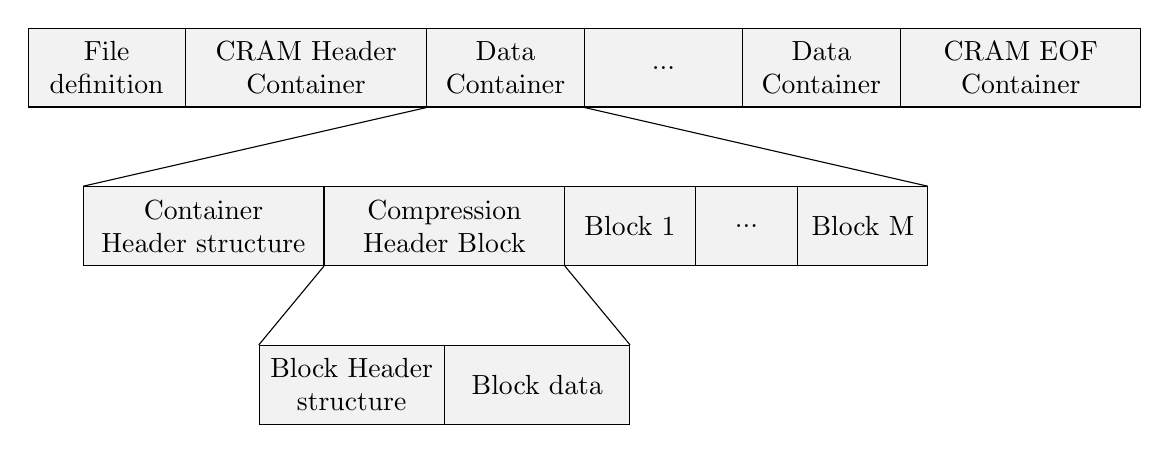
\begin{tikzpicture}[
  every node/.style={scale=1.0},
  boxes/.style={rectangle split,rectangle split parts=#1,draw,rectangle split horizontal,text width=5em,align=center,minimum height=1cm,fill=black!5,on grid},
  notes/.style={text width=20em,align=center,minimum height=1cm,on grid},
]
\node (file) [boxes=6] {
\nodepart{one}File definition
\nodepart[text width=8em]{two}CRAM Header Container
\nodepart{three}Data Container
\nodepart{four}...
\nodepart{five}Data Container
\nodepart[text width=8em]{six}CRAM EOF Container
};

\node (container) [boxes=5,below=1 of file.three south,text width=8em] {
\nodepart{one}Container Header structure
\nodepart{two}Compression Header Block
\nodepart[text width=4em]{three}Block 1
\nodepart[text width=3em]{four}...
\nodepart[text width=4em]{five}Block M
};
\draw (file.two split south) to (container.north west);
\draw (file.three split south) to (container.north east);

\node (blocks) [boxes=2,below=1 of container.two south,text width=6em] {
\nodepart{one}Block Header structure
\nodepart{two}Block data
};
\draw (container.one split south) to (blocks.north west);
\draw (container.two split south) to (blocks.north east);
\end{tikzpicture}

Figure 3: Containers as a series of blocks
\end{center}

The blocks after the compression header are organised logically into slices. One 
slice may contain, for example, a contiguous region of alignment data. Slices begin 
with a slice header block and are followed by one or more data blocks.
It is these data blocks which hold the primary bulk of CRAM data.
The data blocks are further subdivided into a core data block and one or more external data blocks.

\begin{center}
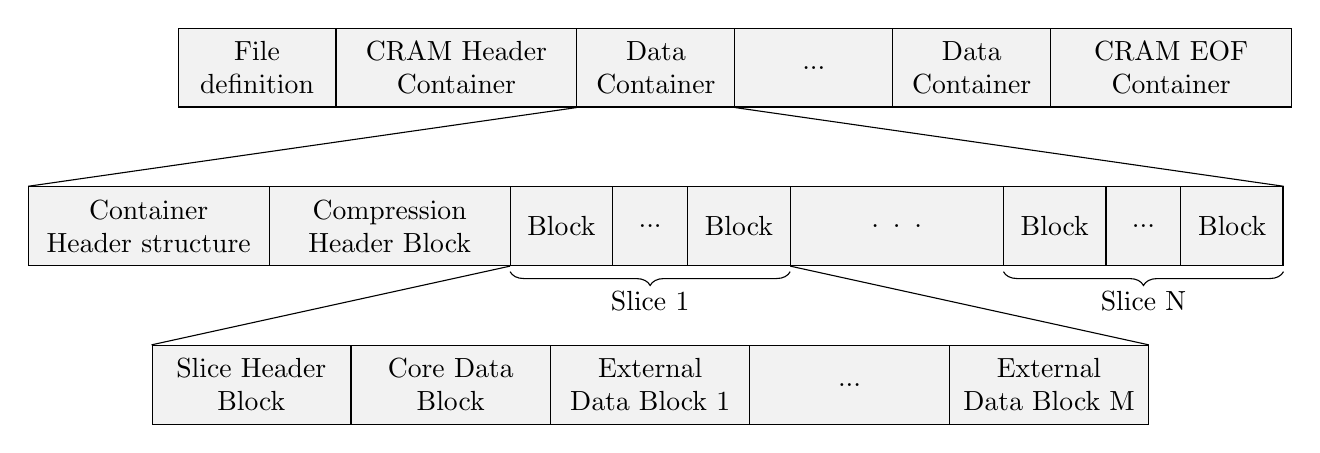
\begin{tikzpicture}[
  every node/.style={scale=1.0},
  boxes/.style={rectangle split,rectangle split parts=#1,draw,rectangle split horizontal,text width=5em,align=center,minimum height=1cm,fill=black!5,on grid},
  notes/.style={text width=20em,align=center,minimum height=1cm,on grid},
]
\node (file) [boxes=6] {
\nodepart{one}File definition
\nodepart[text width=8em]{two}CRAM Header Container
\nodepart{three}Data Container
\nodepart{four}...
\nodepart{five}Data Container
\nodepart[text width=8em]{six}CRAM EOF Container
};

\node (container) [boxes=9,below=1 of file.three south,text width=8em] {
\nodepart{one}Container Header structure
\nodepart{two}Compression Header Block
\nodepart[text width=3em]{three}Block
\nodepart[text width=2em]{four}...
\nodepart[text width=3em]{five}Block
\nodepart[text width=7em]{six}. . .
\nodepart[text width=3em]{seven}Block
\nodepart[text width=2em]{eight}...
\nodepart[text width=3em]{nine}Block
};
\draw (file.two split south) to (container.north west);
\draw (file.three split south) to (container.north east);

\draw[decoration={brace,mirror,amplitude=5pt,raise=2pt},decorate]
  (container.two split south) to (container.five split south);
\node [below=0.2 of container.four south] {Slice 1};

\draw[decoration={brace,mirror,amplitude=5pt,raise=2pt},decorate]
  (container.six split south) to (container.south east);
\node [below=0.2 of container.eight south] {Slice N};

\node (slice) [boxes=5,below=1 of container.four south, text width=6.5em] {
\nodepart{one}Slice Header Block
\nodepart{two}Core Data Block
\nodepart{three}External Data Block 1
\nodepart{four}...
\nodepart{five}External Data Block M
};
\draw (container.two split south) to (slice.north west);
\draw (container.five split south) to (slice.north east);
\end{tikzpicture}

Figure 4: Slices formed from a series of concatenated blocks
\end{center}

\section{\textbf{File definition}}

Each CRAM file starts with a fixed length (26 bytes) definition with the following 
fields:

\begin{tabular}{|l|l|l|}
\hline
\textbf{Data type} & \textbf{Name} & \textbf{Value}\tabularnewline
\hline
byte[4] & format magic number & CRAM (0x43 0x52 0x41 0x4d)\tabularnewline
\hline
unsigned byte & major format number & 3 (0x3)\tabularnewline
\hline
unsigned byte & minor format number & 1 (0x1)\tabularnewline
\hline
byte[20] & file id & CRAM file identifier (e.g. file name or SHA1 checksum)\tabularnewline
\hline
\end{tabular}

Valid CRAM \textit{major}.\textit{minor} version numbers are as follows:

\begin{itemize}
\item[\textit{1.0}]
The original public CRAM release.

\item[\textit{2.0}]
The first CRAM release implemented in both Java and C; tidied up
implementation vs specification differences in \textit{1.0}.

\item[\textit{2.1}]
Gained end of file markers; compatible with \textit{2.0}.

\item[\textit{3.0}]
Additional compression methods; header and data checksums;
improvements for unsorted data.

\item[\textit{3.1}]
Additional EXTERNAL compression codecs only.
\end {itemize}

CRAM 3.0 and 3.1 differ only in the list of compression
methods available, so tools that output CRAM 3 without using any 3.1
codecs should write the header to indicate 3.0 in order to permit
maximum compatibility.

\section{\textbf{Container header structure}}
\label{sec:container}

The file definition is followed by one or more containers with the following header 
structure where the container content is stored in the `blocks' field:

\begin{tabular}{|l|>{\raggedright}p{120pt}|>{\raggedright}p{260pt}|}
\hline
\textbf{Data type} & \textbf{Name} & \textbf{Value}
\tabularnewline
\hline
int32 & length & the sum of the lengths of all blocks in this container (headers and data); 
equal to the total byte length of the container minus the byte length of this header structure\tabularnewline
\hline
itf8 & reference sequence id & reference sequence identifier  or\linebreak{}
-1 for unmapped reads\linebreak{}
-2 for multiple reference sequences.\linebreak{}
All slices in this container must have a reference sequence id matching this value.\tabularnewline
\hline
itf8 & starting position on the reference & the alignment start position\tabularnewline
\hline
itf8 & alignment span & the length of the alignment\tabularnewline
\hline
itf8 & number of records & number of records in the container\tabularnewline
\hline
ltf8 & record counter & 1-based sequential index of records in the file/stream.\tabularnewline
\hline
ltf8 & bases & number of read bases\tabularnewline
\hline
itf8 & number of blocks & the total number of blocks in this container\tabularnewline
\hline
array\texttt{<}itf8\texttt{>} & landmarks & the locations of slices in this container as byte offsets from the end of
this container header, used for random access indexing.
For sequence data containers, the landmark count must equal the slice count.\linebreak{}
Since the block before the first slice is the compression header,
landmarks[0] is equal to the byte length of the compression header.\tabularnewline
\hline
int & crc32 & CRC32 hash of the all the preceding bytes in the container.\tabularnewline
\hline
byte[ ] & blocks & The blocks contained within the container.\tabularnewline
\hline
\end{tabular}

In the initial CRAM header container, the reference sequence id,
starting position on the reference, and alignment span fields must be
ignored when reading. The landmarks array is optional for the CRAM
header, but if it exists it should point to block offsets instead of
slices, with the first block containing the textual header.

In data containers specifying unmapped reads or multiple reference
sequences (i.e. reference sequence id $< 0$), the starting position on
the reference and alignment span fields must be ignored when
reading. When writing, it is recommended to set each of these ignored
fields to the value 0.


\subsection{\textbf{CRAM header container}}
\label{subsec:cram-header-container}

The first container in a CRAM file contains a textual header in one or more blocks.  See section~\ref{subsec:header-block} for more details on the layout of data within these blocks and constraints applied to the contents of the SAM header.

The landmarks field of the container header structure may be used to
indicate the offsets of the blocks used in the header container.
These may optionally be omitted by specifying an array size of zero.

\section{\textbf{Block structure}}
\label{sec:block-struct}

Containers consist of one or more blocks. Block compression is applied independently 
and in addition to any encodings used to compress data within the block. The block 
have the following header structure with the data stored in the `block data' field:

\begin{tabular}{|l|>{\raggedright}p{120pt}|>{\raggedright}p{260pt}|}
\hline
\textbf{Data type} & \textbf{Name} & \textbf{Value}
\tabularnewline
\hline
byte & method & the block compression method (and first CRAM version): \linebreak{}
0: raw (none)*\linebreak{}
1: gzip\linebreak{}
2: bzip2 (v2.0)\linebreak{}
3: lzma (v3.0)\linebreak{}
4: rans4x8 (v3.0)\linebreak{}
5: rans4x16 (v3.1)\linebreak{}
6: adaptive arithmetic coder (v3.1)\linebreak{}
7: fqzcomp (v3.1)\linebreak{}
8: name tokeniser (v3.1)
\tabularnewline
\hline
byte & block content type id & the block content type identifier\tabularnewline
\hline
itf8 & block content id & the block content identifier used to associate external 
data blocks with data series\tabularnewline
\hline
itf8 & size in bytes* & size of the block data after applying block compression\tabularnewline
\hline
itf8 & raw size in bytes* & size of the block data before applying block compression\tabularnewline
\hline
byte[ ] & block data & the data stored in the block:\linebreak{}
$\bullet$ bit stream of CRAM records (core data block)\linebreak{}
$\bullet$ byte stream (external data block)\linebreak{}
$\bullet$ additional fields ( header blocks)\tabularnewline
\hline
byte[4] & CRC32 & CRC32 hash value for all preceding bytes in the block\tabularnewline
\hline
\end{tabular}

* Note on raw method: both compressed and raw sizes must be set to the same value.

Empty blocks may occur in the files.
Blocks with a raw (uncompressed) size of zero are treated as empty,
irrespective of their ``method'' byte.  This is equivalent to
interpreting them as having method zero (raw) and compressed size of
zero.

\subsection{\textbf{Block content types}}

CRAM has the following block content types:

\begin{threeparttable}[t]
\begin{tabular}{|>{\raggedright}p{143pt}|>{\raggedright}p{45pt}|>{\raggedright}p{116pt}|>{\raggedright}p{114pt}|}
\hline
\textbf{Block content type} & \textbf{Block content type id} & \textbf{Name} & \textbf{Contents}\tabularnewline
\hline
FILE\_HEADER & 0 & CRAM header block & CRAM header\tabularnewline
\hline
COMPRESSION\_HEADER & 1 & Compression header block & See specific section\tabularnewline
\hline
SLICE\_HEADER\tnote{a} & 2 & Slice header block & See specific section\tabularnewline
\hline
 & 3 &  & reserved\tabularnewline
\hline
EXTERNAL\_DATA & 4 & external data block & data produced by external encodings\tabularnewline
\hline
CORE\_DATA & 5 & core data block & bit stream of all encodings except for external encodings\tabularnewline
\hline
\end{tabular}
\begin{tablenotes}
\item[a] Formerly MAPPED\_SLICE\_HEADER.  Now used by all slice headers regardless of mapping status.
\end{tablenotes}
\end{threeparttable}

\subsection{\textbf{Block content id}}

Block content id is used to distinguish between external blocks in the same slice. 
Each external encoding has an id parameter which must be one of the external block 
content ids. For external blocks the content id is a positive integer. For all 
other blocks content id should be 0. Consequently, all external encodings must 
not use content id less than 1. 

\subsubsection*{Data blocks}

Data is stored in data blocks. There are two types of data blocks: core data blocks 
and external data blocks.The difference between core and external data blocks is 
that core data blocks consist of data series that are compressed using bit encodings 
while the external data blocks are byte compressed. One core data block and any 
number of external data blocks are associated with each slice.

Writing to and reading from core and external data blocks is organised through 
CRAM records. Each data series is associated with an encoding. In case of external 
encodings the block content id is used to identify the block where the data series 
is stored. Please note that external blocks can have multiple data series associated 
with them; in this case the values from these data series will be interleaved. 


\subsection{\textbf{CRAM header block(s)}}
\label{subsec:header-block}

The SAM header is stored in the first block of the CRAM header container (see section~\ref{subsec:cram-header-container}).
This block may be uncompressed or gzip compressed only.
This block is followed by zero or more uncompressed expansion blocks.
If present, these permit in-place editing of the CRAM header, allowing it to grow or shrink with a compensatory size change applied to the subsequence expansion block, avoiding the need to rewrite the remainder of the file.
The contents of any expansion blocks should be zero bytes (nul characters).

The format of the initial SAM header block is a 32-bit little-endian integer holding the length of the text of the SAM header, minus nul-termination bytes, followed by the text itself.
Although 32-bit, the maximum permitted value is $2^{31}$, and all lengths must be positive.

The following constraints apply to the SAM header text: 

\begin{itemize}
\item The SQ:MD5 checksum is required unless the reference sequence has been embedded 
into the file.
\end{itemize}

\subsection{\textbf{Compression header block}}
\label{subsec:compression-header}

The compression header block consists of 3 parts: preservation map, data series 
encoding map and tag encoding map.

\subsubsection*{Preservation map}

The preservation map contains information about which data was preserved in the 
CRAM file. It is stored as a map with byte[2] keys:

\begin{tabular}{|l|l|>{\raggedright}p{100pt}|>{\raggedright}p{220pt}|}
\hline
\textbf{Key} & \textbf{Value data type} & \textbf{Name} & \textbf{Value}\tabularnewline
\hline
RN & bool & read names included & true if read names are preserved for all reads\tabularnewline
\hline
AP & bool & AP data series delta & true if AP data series is delta, false otherwise\tabularnewline
\hline
RR & bool & reference required & true if reference sequence is required to restore 
the data completely\tabularnewline
\hline
SM & byte[5] & substitution matrix & substitution matrix\tabularnewline
\hline
TD & array\texttt{<}byte\texttt{>} & tag ids dictionary & a list of lists of tag ids, see tag encoding section\tabularnewline
\hline
\end{tabular}

The boolean values are optional, defaulting to true when absent, although it is recommended to explicitly set them.  SM and TD are mandatory.

\subsubsection*{Data series encodings}

Each data series has an encoding. These encoding are stored in a map with byte[2] 
keys and are decoded in approximately this order\footnote{The precise order is defined in section~\ref{sec:record}.}:

\begin{threeparttable}[t]
\begin{tabular}{|l|l|>{\raggedright}p{100pt}|>{\raggedright}p{220pt}|}
\hline
\textbf{Key} & \textbf{Value data type} & \textbf{Name} & \textbf{Value}\tabularnewline
\hline
BF & encoding\texttt{<}int\texttt{>} & BAM bit flags & see separate section\tabularnewline
\hline
CF & encoding\texttt{<}int\texttt{>} & CRAM bit flags & see specific section\tabularnewline
\hline
RI & encoding\texttt{<}int\texttt{>} & reference id & record reference id from
the SAM file header\tabularnewline
\hline
RL & encoding\texttt{<}int\texttt{>} & read lengths & read lengths\tabularnewline
\hline
AP & encoding\texttt{<}int\texttt{>} & in-seq positions & if \textbf{AP-Delta} = true: 0-based alignment start
delta from the AP value in the previous record.
Note this delta may be negative, for example when switching references in a multi-reference slice.
When the record is the first in the slice, the previous position used is the slice alignment-start field (hence the first delta should be zero for single-reference slices, or the AP value itself for multi-reference slices).  \linebreak{}
if \textbf{AP-Delta} = false: encodes the alignment start position directly\tabularnewline
\hline
RG & encoding\texttt{<}int\texttt{>} & read groups & read groups. Special value 
`-1' stands for no group.\tabularnewline
\hline
RN\tnote{a} & encoding\texttt{<}byte[ ]\texttt{>} & read names & read names\tabularnewline
\hline
MF & encoding\texttt{<}int\texttt{>} & next mate bit flags & see specific section\tabularnewline
\hline
NS & encoding\texttt{<}int\texttt{>} & next fragment reference sequence id & reference 
sequence ids for the next fragment \tabularnewline
\hline
NP & encoding\texttt{<}int\texttt{>} & next mate alignment start & alignment positions 
for the next fragment\tabularnewline
\hline
TS & encoding\texttt{<}int\texttt{>} & template size & template sizes\tabularnewline
\hline
NF & encoding\texttt{<}int\texttt{>} & distance to next fragment & number of records
to skip to the next fragment\tnote{b}\tabularnewline
\hline
TL\tnote{c} & encoding\texttt{<}int\texttt{>} & tag ids  & list of tag ids, see tag encoding
section\tabularnewline
\hline
FN & encoding\texttt{<}int\texttt{>} & number of read features & number of read
features in each record\tabularnewline
\hline
FC & encoding\texttt{<}byte\texttt{>} & read features codes & see separate section\tabularnewline
\hline
FP & encoding\texttt{<}int\texttt{>} & in-read positions & positions of the read
features; a positive delta to the last position (starting with zero)\tabularnewline
\hline
DL & encoding\texttt{<}int\texttt{>} & deletion lengths & base-pair deletion lengths\tabularnewline
\hline
BB & encoding\texttt{<}byte[ ]\texttt{>} & stretches of bases & bases\tabularnewline
\hline
QQ & encoding\texttt{<}byte[ ]\texttt{>} & stretches of quality scores & quality scores\tabularnewline
\hline
BS & encoding\texttt{<}byte\texttt{>} & base substitution codes & base substitution
codes\tabularnewline
\hline
IN & encoding\texttt{<}byte[ ]\texttt{>} & insertion & inserted bases\tabularnewline
\hline
RS & encoding\texttt{<}int\texttt{>} & reference skip length & number of skipped 
bases for the `N' read feature\tabularnewline
\hline
PD & encoding\texttt{<}int\texttt{>} & padding & number of padded bases\tabularnewline
\hline
HC & encoding\texttt{<}int\texttt{>} & hard clip & number of hard clipped bases\tabularnewline
\hline
SC & encoding\texttt{<}byte[ ]\texttt{>} & soft clip & soft clipped bases\tabularnewline
\hline
MQ & encoding\texttt{<}int\texttt{>} & mapping qualities & mapping quality scores\tabularnewline
\hline
BA & encoding\texttt{<}byte\texttt{>} & bases & bases\tabularnewline
\hline
QS & encoding\texttt{<}byte\texttt{>} & quality scores & quality scores\tabularnewline
\hline
TC\tnote{d} & N/A & legacy field & to be ignored\tabularnewline
\hline
TN\tnote{d} & N/A & legacy field & to be ignored\tabularnewline
\end{tabular}

\begin{tablenotes}
\item[a] Note RN this is decoded after MF if the record is detached from the mate and we are attempting to auto-generate read names.
\item[b] The count is reset for each slice so NF can only refer to a record later within this slice.
\item[c] TL is followed by decoding the tag values themselves, in order of appearance in the tag dictionary.
\item[d] TC and TN are legacy data series from CRAM 1.0.
They have no function in CRAM 3.0 and should not be present.
However some implementations do output them and decoders must silently skip these fields.
It is illegal for TC and TN to contain any data values, although there
may be empty blocks associated with them.
\end{tablenotes}
\end{threeparttable}

\subsubsection*{Tag encodings}
\label{subsubsec:tags}

The tag dictionary (TD) describes the unique combinations of tag id / type that occur on each alignment record.
For example if we search the id / types present in each record and find only two combinations -- X1:i BC:Z SA:Z: and X1:i: BC:Z -- then we have two dictionary entries in the TD map.

Let $L_{i}=\{T_{i0}, T_{i1}, \ldots, T_{ix}\}$ be a list of all tag ids for a record $R_{i}$, where $i$ is the sequential record index and $T_{ij}$ denotes $j$-th tag id in the record.
The list of unique $L_{i}$ is stored as the TD value in the preservation map.
Maintaining the order is not a requirement for encoders (hence ``combinations''), but it is permissible and thus different permutations, each encoded with their own elements in TD, should be supported by the decoder.
Each $L_{i}$ element in TD is assigned a sequential integer number starting with 0.
These integer numbers are referred to by the TL data series.
Using TD, an integer from the TL data series can be mapped back into a list of tag ids.
Thus per alignment record we only need to store tag values and not their ids and types.

The TD is written as a byte array consisting of $L_{i}$ values separated with \textbackslash{}0.
Each $L_{i}$ value is written as a concatenation of 3 byte $T_{ij}$ elements: tag id followed by BAM tag type code (one of A, c, C, s, S, i, I, f, F, Z, H or B, as described in the SAM specification).
For example the TD for tag lists X1:i BC:Z SA:Z and X1:i BC:Z may be encoded as X1CBCZSAZ\textbackslash{}0X1CBCZ\textbackslash{}0, with X1C indicating a 1 byte unsigned value for tag X1.

\subsubsection*{Tag values}

The encodings used for different tags are stored in a map.
The key is 3 bytes formed from the BAM tag id and type code, matching the TD dictionary described above.
Unlike the Data Series Encoding Map, the key is stored in the map as an ITF8 encoded integer, constructed using $(char1<<16) + (char2<<8) + type$.
For example, the 3-byte representation of OQ:Z is \{0x4F, 0x51, 0x5A\} and these bytes are interpreted as the integer key 0x004F515A, leading to an ITF8 byte stream \{0xE0, 0x4F, 0x51, 0x5A\}.

\begin{tabular}{|l|l|l|>{\raggedright}p{160pt}|}
\hline
\textbf{Key} & \textbf{Value data type} & \textbf{Name} & \textbf{Value}
\tabularnewline
\hline
TAG ID 1:TAG TYPE 1 & encoding\texttt{<}byte[ ]\texttt{>} & read tag 1 & tag values
(names and types are available in the data series code)\tabularnewline
\hline
... &  & ... & ...\tabularnewline
\hline
TAG ID N:TAG TYPE N & encoding\texttt{<}byte[ ]\texttt{>} & read tag N & ...\tabularnewline
\hline
\end{tabular}

Note that tag values are encoded as array of bytes. The routines to convert tag 
values into byte array and back are the same as in BAM with the exception of value 
type being captured in the tag key rather in the value.
Hence consuming 1 byte for types `C' and `c', 2 bytes for types `S' and `s', 4 bytes for types `I', `i' and `f', and a variable number of bytes for types `H', `Z' and `B'.

\subsection{\textbf{Slice header block}}

The slice header block is never compressed (block method=raw). For reference mapped 
reads the slice header also defines the reference sequence context of the data 
blocks associated with the slice. Mapped reads can be stored along with
\textbf{placed unmapped}\footnote{Unmapped reads can be \textit{placed} or \textit{unplaced}.
By placed unmapped read we mean a read that is unmapped according to bit 0x4 of the
BF (BAM bit flags) data series, but has position fields filled in, thus "placing"  it on a reference sequence. In contrast,
unplaced unmapped reads have have a reference sequence ID of -1 and alignment position of 0.}
reads on the same reference within the same slice.

Slices with the Multiple Reference flag (-2) set as the sequence ID in the header may contain reads
mapped to multiple external references, including unmapped\footnotemark[\value{footnote}] reads (placed on these references or unplaced),
but multiple embedded references cannot be combined in this way.  When multiple references are
used, the RI data series will be used to determine the reference sequence ID for each record.  This
data series is not present when only a single reference is used within a slice.

The Unmapped (-1) sequence ID in the header is for slices containing only unplaced
unmapped\footnotemark[\value{footnote}] reads.

A slice containing data that does not use the external reference in
any sequence may set the reference MD5 sum to zero.  This can happen
because the data is unmapped or the sequence has been stored verbatim
instead of via reference-differencing.  This latter scenario is
recommended for unsorted or non-coordinate-sorted data.

The slice header block contains the following fields.

\begin{tabular}{|l|l|>{\raggedright}p{200pt}|}
\hline
\textbf{Data type} & \textbf{Name} & \textbf{Value}\tabularnewline
\hline
itf8 & reference sequence id & reference sequence identifier or\linebreak{}
-1 for unmapped reads\linebreak{}
-2 for multiple reference sequences.\linebreak{}
This value must match that of its enclosing container.\tabularnewline
\hline
itf8 & alignment start & the alignment start position\tabularnewline
\hline
itf8 & alignment span & the length of the alignment\tabularnewline
\hline
itf8 & number of records & the number of records in the slice\tabularnewline
\hline
ltf8 & record counter & 1-based sequential index of records in the file/stream\tabularnewline
\hline
itf8 & number of blocks & the number of blocks in the slice\tabularnewline
\hline
itf8[ ] & block content ids & block content ids of the blocks in the slice\tabularnewline
\hline
itf8 & embedded reference bases block content id & block content id for the embedded 
reference sequence bases or -1 for none\tabularnewline
\hline
byte[16] & reference md5 & MD5 checksum of the reference bases within the slice 
boundaries.  If this slice has reference sequence id of -1 (unmapped) or -2 (multi-ref)
the MD5 should be 16 bytes of \textbackslash{}0. For embedded references, the MD5
can either be all-zeros or the MD5 of the embedded sequence.\tabularnewline
\hline
byte[ ] & optional tags & a series of tag,type,value tuples encoded as
per BAM auxiliary fields.\tabularnewline
\hline
\end{tabular}

The alignment start and alignment span values should only be utilised
during decoding if the slice has mapped data aligned to a single
reference (reference sequence id $>= 0$).  For multi-reference slices
or those with unmapped data, it is recommended to fill these fields
with value 0.

MD5sums should not be validated if the stored checksum is all-zero.
Embedded references should follow the same capitalisation and
alphabetical rules as applied to external references prior to MD5sum
calculations. If an embedded reference is used, it is not a
requirement that it exactly matches the reference used for sequence
alignments.  For example, it may contain ``N'' bases where coverage is
absent or it could have different base calls for SNP variants.  Hence
when embedded sequences are used, the MD5sum refers to the checksum of
the embedded sequence and should not be validated against any external
reference files.

Note where an embedded reference differs to the original reference
used for alignment, the MD and NM tags may need to be stored verbatim
for records where the respective embedded and external reference
substrings differ.

The optional tags are encoded in the same manner as BAM tags.  I.e. a
series of binary encoded tags concatenated together where each tag
consists of a 2 byte key (matching [A-Za-z][A-Za-z0-9]) followed by a
1 byte type ([AfZHcCsSiIB]) followed by a string of bytes in a format
defined by the type.

Tags starting in a capital letter are reserved while lowercase ones or
those starting with X, Y or Z are user definable.  Any tag not
understood by a decoder should be skipped over without producing an
error.

At present no tags are defined.

% Details omitted until we fully work through all the corner cases,
% such as seq/qual of *.
%
% Reserved tags are defined as follows:
% 
% \begin{tabular}{|l|l|>{\raggedright}p{325pt}|}
% \hline
% \textbf{Tag type} & \textbf{BAM format} & \textbf{Meaning}\tabularnewline
% \hline
% BD & i & Sum over all reads of the CRC32 hash of sequence base.  This
% may be used to validate round-trips in and out of CRAM.
% calls\tabularnewline
% \hline
% SD & i & Sum over all reads of the CRC32 hash of quality scores. (If
% the quality string is ``*'' in SAM then the hash is of the BAM encoded
% version - a string of bytes with value 255.)\tabularnewline
% \hline
% \end{tabular}


\subsection{\textbf{Core data block}}

A core data block is a bit stream (most significant bit first) consisting of data from one 
or more CRAM records. Please note that one byte could hold more then one CRAM record 
as a minimal CRAM record could be just a few bits long. The core data block has 
the following fields:

\begin{tabular}{|l|>{\raggedright}p{120pt}|>{\raggedright}p{260pt}|}
\hline
\textbf{Data type} & \textbf{Name} & \textbf{Value}
\tabularnewline
\hline
bit[ ] & CRAM record 1 & The first CRAM record\tabularnewline
\hline
... & ... & ...\tabularnewline
\hline
bit[ ] & CRAM record N & The Nth CRAM record \tabularnewline
\hline
\end{tabular}

\subsection{\textbf{External data blocks}}

The relationship between the core data block and external data blocks is shown in the following 
picture: 

\begin{center}
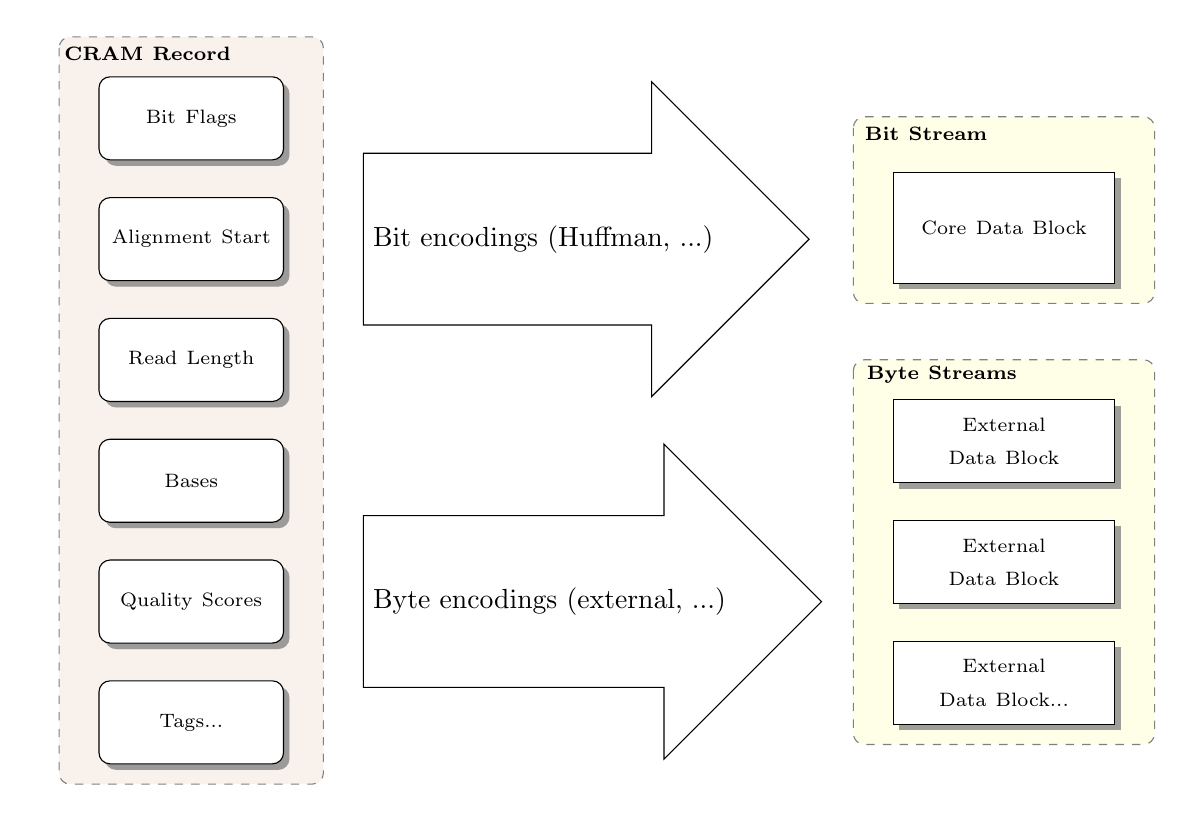
\begin{tikzpicture}

\usetikzlibrary{shapes, shadows, positioning, arrows,  decorations.markings}

\pgfdeclarelayer{background}
\pgfsetlayers{background,main}

\tikzstyle{dsbox} = [blockbox, text width=6em, minimum width=6em, minimum height=3em, rounded corners, drop shadow]
\tikzstyle{blockbox}=[draw, fill=white, text width=4.0em, text centered, minimum height=1.0em, drop shadow]
\tikzstyle{encodedblocklarge} = [blockbox, text width=6em, minimum width=8em, minimum height=4em, drop shadow]
\tikzstyle{encodedblock} = [blockbox, text width=6em, minimum width=8em, minimum height=3em, drop shadow]

\tikzstyle{texto} = [above, text width=8em, text centered]

\newcommand{\cramRecord}[6]{%
\begin{pgfonlayer}{background}
    \path (#1.west |- #1.north) + (-0.5, 0.5) node (a1) {};
    \path (#1.east |- #6.south) + (+0.5,-0.25) node (a2) {};
    \path[fill=brown!10,rounded corners, draw=black!50, dashed]
      (a1) rectangle (a2);
    \path (a1.east |- a1.south) + (1.0,-0.3) node[texto]
      {\scriptsize\textbf{CRAM Record}};
\end{pgfonlayer}}

\newcommand{\dsbox}[2]{node (p#1) [dsbox]
{\scriptsize{#2}}}
\newcommand{\encodedblock}[2]{node (p#1) [encodedblock]
	{\scriptsize{#2}}}
\newcommand{\encodedblocklarge}[2]{node (p#1) [encodedblocklarge]
   {\scriptsize{#2}}}

\path +(-2.5,-1.5) \dsbox{1}{Bit Flags};
\path (p1.south)+(0.0,-1.0) \dsbox{2}{Alignment Start};
\path (p2.south)+(0.0,-1.0) \dsbox{3}{Read Length};
\path (p3.south)+(0.0,-1.0) \dsbox{4}{Bases};
\path (p4.south)+(0.0,-1.0) \dsbox{5}{Quality Scores};
\path (p5.south)+(0.0,-1.0) \dsbox{6}{Tags...};

\cramRecord{p1}{p2}{p3}{p4}{p5}{p6}

\newcommand{\blockStreams}[4]{%
\begin{pgfonlayer}{background}
    \path (#1.west |- #1.north)+(-0.5, .7) node (a1) {};
    \path (#1.east |- #1.south)+(+0.5, -0.25) node (a2) {};
    \path (#2.west |- #2.north)+(-0.5, 0.5) node (a3) {};
    \path (#4.east |- #4.south)+(+0.5, -0.25) node (a4) {};
    \path[fill=yellow!10, rounded corners, draw=black!50, dashed]
      (a1) rectangle (a2);
    \path (a1.east |- a1.south)+(0.8,-0.3) node[texto]
      {\scriptsize\textbf{Bit Stream}};
    \path[fill=yellow!10, rounded corners, draw=black!50, dashed]
      (a3) rectangle (a4);
    \path (a3.east |- a3.south)+(1.0,-0.3) node[texto]{\scriptsize\textbf{Byte Streams}};
\end{pgfonlayer}}

\path (a1.south) + (12.0, -2.3) \encodedblocklarge {7} {Core Data Block};
\path (p7.south) + (0.0, -2.0) \encodedblock {8} {External Data Block};
\path (p8.south) + (0.0, -1.0) \encodedblock {9} {External Data Block}; 
\path (p9.south) + (0.0, -1.0) \encodedblock {10}{External Data Block...};

\blockStreams {p7} {p8} {p9} {p10}

\node[minimum size=4cm, right = of p2, single arrow, draw, single arrow head indent=0ex, black] {Bit encodings (Huffman, ...) };

\node[minimum size=4cm, right = of p5, single arrow, draw, single arrow head indent=0ex, black] {Byte encodings (external, ...) };

\end{tikzpicture}

Figure 5: The relationship between core and external encodings, and core and external data blocks.

\end{center}

The picture shows how a CRAM record (on the left) is distributed between the core 
data block and one or more external data blocks, via core or external encodings. The specific 
encodings presented are only examples for purposes of illustration. The main point is 
to distinguish between core bit encodings whose output is always stored in a core data 
block, and external byte encodings whose output is always stored in external data 
blocks.

\section{\textbf{End of file container}}

A special container is used to mark the end of a file or stream. It is required in version 3 or later. The idea is to provide an easy and a quick way to detect that a CRAM file or stream is complete. The marker is basically an empty container with ref seq id set to -1 (unaligned) and alignment 
start set to 4542278.

Here is a complete content of the EOF container explained in detail:

\begin{tabular}{|l|l|>{\raggedright}p{150pt}|>{\raggedright}p{180pt}|}
\hline
\textbf{hex bytes} & \textbf{data type} & \textbf{decimal value} & \textbf{field 
name}\tabularnewline
\hline
\multicolumn{4}{|l|}{\textit{Container header}}\tabularnewline
\hline
0f 00 00 00 & integer & 15 & size of blocks data\tabularnewline
\hline
ff ff ff ff 0f & itf8 & -1 & ref seq id\tabularnewline
\hline
e0 45 4f 46 & itf8 & 4542278 & alignment start\tabularnewline
\hline
00 & itf8 & 0 & alignment span\tabularnewline
\hline
00 & itf8 & 0 & number of records\tabularnewline
\hline
00 & itf8 & 0 & global record counter\tabularnewline
\hline
00 & itf8 & 0 & bases\tabularnewline
\hline
01 & itf8 & 1 & block count\tabularnewline
\hline
00 & array & 0 & landmarks\tabularnewline
\hline
05 bd d9 4f & integer & 1339669765 & container header CRC32\tabularnewline
\hline
\multicolumn{4}{|l|}{\textit{Compression header block}}\tabularnewline
\hline
00 & byte & 0 (RAW) & compression method\tabularnewline
\hline
01 & byte & 1 (COMPRESSION\_HEADER) & block content type\tabularnewline
\hline
00 & itf8 & 0 & block content id\tabularnewline
\hline
06 & itf8 & 6 & compressed size\tabularnewline
\hline
06 & itf8 & 6 & uncompressed size\tabularnewline
\hline
\multicolumn{4}{|l|}{\textit{Compression header}}\tabularnewline
\hline
01 & itf8 & 1 & preservation map byte size\tabularnewline
\hline
00 & itf8 & 0 & preservation map size\tabularnewline
\hline
01 & itf8 & 1 & encoding map byte size\tabularnewline
\hline
00 & itf8 & 0 & encoding map size\tabularnewline
\hline
01 & itf8 & 1 & tag encoding byte size\tabularnewline
\hline
00 & itf8 & 0 & tag encoding map size\tabularnewline
\hline
ee 63 01 4b & integer & 1258382318 & block CRC32\tabularnewline
\hline
\end{tabular}

When compiled together the EOF marker is 38 bytes long and in hex representation 
is:

0f 00 00 00 ff ff ff ff 0f e0 45 4f 46 00 00 00 00 01 00 05 bd d9 4f 00 01 00 06 06 01 00 01 00 01 00 ee 63 01 4b

\section{\textbf{Record structure}}
\label{sec:record}

CRAM record is based on the SAM record but has additional features allowing for 
more efficient data storage.  In contrast to BAM record CRAM record uses bits as 
well as bytes for data storage. This way, for example, various coding techniques 
which output variable length binary codes can be used directly in CRAM. On the 
other hand, data series that do not require binary coding can be stored separately 
in external blocks with some other compression applied to them independently.

As CRAM data series may be interleaved within the same blocks\footnote{Interleaving can sometimes provide better compression, however it also adds dependency between types of data meaning it is not possible to selectively decode one data series if it co-locates with another data series in the same block.} understanding the order in which CRAM data series must be decoded is vital.

The overall flowchart is below, with more detailed description in the subsequent sections.

\algnewcommand\algorithmicto{\text{ \textbf{to} }}

\subsection{\textbf{CRAM record}}

Both mapped and unmapped reads start with the following fields. Please note that 
the data series type refers to the logical data type and the data series name corresponds 
to the data series encoding map.

\begin{tabular}{|>{\raggedright}p{70pt}|>{\raggedright}p{75pt}|>{\raggedright}p{90pt}|>{\raggedright}p{171pt}|}
\hline
\textbf{Data series type} & \textbf{Data series name} & \textbf{Field} & \textbf{Description}\tabularnewline
\hline
int & BF & BAM bit flags & see BAM bit flags below\tabularnewline
\hline
int & CF & CRAM bit flags & see CRAM bit flags below\tabularnewline
\hline
- & - & Positional data & See section \ref{subsec:positions}\tabularnewline
\hline
- & - & Read names & See section \ref{subsec:names}\tabularnewline
\hline
- & - & Mate records & See section \ref{subsec:mate}\tabularnewline
\hline
- & - & Auxiliary tags & See section \ref{subsec:tags}\tabularnewline
\hline
- & - & Sequences & See sections \ref{subsec:mapped} and \ref{subsec:unmapped}\tabularnewline
\hline
\end{tabular}

\subsubsection*{\textbf{BAM bit flags (BF data series)}}

The following flags are duplicated from the SAM and BAM specification, with identical meaning.
Note however some of these flags can be derived during decode, so may be omitted in the CRAM file and the bits computed based on both reads of a pair-end library residing within the same slice.

\begin{threeparttable}[t]
\begin{tabular}{|>{\raggedright}p{144pt}|>{\raggedright}p{144pt}|>{\raggedright}p{144pt}|}
\hline
\textbf{Bit flag} & \textbf{Comment} & \textbf{Description}\tabularnewline
\hline
0x1 &  & template having multiple segments in sequencing\tabularnewline
\hline
0x2 &  & each segment properly aligned according to the aligner\tabularnewline
\hline
0x4 &  & segment unmapped\tnote{a}\tabularnewline
\hline
0x8 & calculated\tnote{b}\ \ or stored in the mate's info & next segment in template unmapped\tabularnewline
\hline
0x10 &  & SEQ being reverse complemented\tabularnewline
\hline
0x20 & calculated\tnote{b}\ \ or stored in the mate's info & SEQ of the next segment in the
template being reverse complemented\tabularnewline
\hline
0x40 &  & the first segment in the template\tnote{c}\tabularnewline
\hline
0x80 &  & the last segment in the template\tnote{c}\tabularnewline
\hline
0x100 &  & secondary alignment\tabularnewline
\hline
0x200 &  & not passing quality controls\tabularnewline
\hline
0x400 &  & PCT or optical duplicate\tabularnewline
\hline
0x800 &  & Supplementary alignment\tabularnewline
\hline
\end{tabular}
\begin{tablenotes}
\item[a] Bit 0x4 is the only reliable place to tell whether the read is unmapped.  If 0x4 is set, no assumptions may be made about bits 0x2, 0x100 and 0x800.
\item[b] For segments within the same slice.
\item[c] Bits 0x40 and 0x80 reflect the read ordering within each template inherent in the sequencing technology used, which may be independent from the actual mapping orientation.
If 0x40 and 0x80 are both set, the read is part of a linear template (one where the template sequence is expected to be in a linear order), but it is neither the first nor the last read.
If both 0x40 and 0x80 are unset, the index of the read in the template is unknown.
This may happen for a non-linear template (such as one constructed by stitching together other templates) or when this information is lost during data processing.
\end{tablenotes}
\end{threeparttable}

\subsubsection*{\textbf{CRAM bit flags (CF data series)}}

The CRAM bit flags (also known as compression bit flags) expressed as an integer represent the CF data series. 
The following compression flags are defined for each CRAM read record:

\begin{tabular}{|>{\raggedright}p{39pt}|>{\raggedright}p{150pt}|>{\raggedright}p{242pt}|}
\hline
\textbf{Bit flag} & \textbf{Name} & \textbf{Description}\tabularnewline
\hline
0x1 & quality scores stored as array & quality scores can be stored as read features
or as an array similar to read bases.\tabularnewline
\hline
0x2 & detached & mate information is stored verbatim (e.g. because the pair spans multiple slices or the fields differ to the CRAM computed method)\tabularnewline
\hline
0x4 & has mate downstream & tells if the next segment should be expected further
in the stream\tabularnewline
\hline
0x8 & decode sequence as ``*'' & informs the decoder that the sequence
is unknown and that any encoded reference differences are present only to
recreate the CIGAR string.\tabularnewline
\hline
\end{tabular}


The following pseudocode describes the general process of decoding an entire CRAM record.
The sequence data itself is in one of two encoding formats depending on whether the record is aligned (mapped).

\subsubsection*{\textbf{Decode pseudocode}}
\newlength{\maxwidth}
\newcommand{\algalign}[2] % #1 = text to left, #2 = text to right
{\makebox[\maxwidth][l]{$#1{}$}${}#2$}

\begin{algorithmic}[1]
\Procedure{DecodeRecord}{}
\settowidth{\maxwidth}{CRAM\_flags\quad}
\State \algalign{BAM\_flags}{\gets}  \Call{ReadItem}{BF, Integer}
\State \algalign{CRAM\_flags}{\gets} \Call{ReadItem}{CF, Integer}
\State \Call{DecodePositions}{}\Comment{See section \ref{subsec:positions}}
\State \Call{DecodeNames}{}\Comment{See section \ref{subsec:names}}
\State \Call{DecodeMateData}{}\Comment{See section \ref{subsec:mate}}
\State \Call{DecodeTagData}{}\Comment{See section \ref{subsec:tags}}
\Statex

\If{$(BF$ AND $4) \ne 0$}\Comment{Unmapped flag}
  \State \Call{DecodeMappedRead}{}\Comment{See section \ref{subsec:mapped}}
\Else
  \State \Call{DecodeUnmappedRead}{}\Comment{See section \ref{subsec:unmapped}}
\EndIf
\EndProcedure
\end{algorithmic}

This pseudocode is not meant to be a fully implementable programming
language, but to act as an algorithmic guide to the order and
structure of CRAM decoding.

The \textsc{ReadItem} function referred above takes two arguments; the
data series name and the data type used by the Encoding.  It will use
the codec specified in the Container Compression Header to retrieve
the next value from that data series.  Note there is only one
permitted data type per data series, so the second argument is
redundant and is included only as an aide-m\'emoire.

\subsection{\textbf{CRAM positional data}}
\label{subsec:positions}

Following the bit-wise BAM and CRAM flags, CRAM encodes positional related data including reference, alignment positions and length, and read-group.
Positional data is stored for both mapped and unmapped sequences, as unmapped data may still be ``placed'' at a specific location in the genome (without being aligned).
Typically this is done to keep a sequence pair (paired-end or mate-pair sequencing libraries) together when one of the pair aligns and the other does not.

For reads stored in a position-sorted slice, the AP-delta flag in the compression header preservation map should be set and the AP data series will be delta encoded, using the slice alignment-start value as the first position to delta against.
Note for multi-reference slices this may mean that the AP series includes negative values, such as when moving from an alignment to the end of one reference sequence to the start of the next or to unmapped unplaced data.  When the AP-delta flag is not set the AP data series is stored as a normal integer value.

\begin{tabular}{|>{\raggedright}p{70pt}|>{\raggedright}p{75pt}|>{\raggedright}p{90pt}|>{\raggedright}p{171pt}|}
\hline
\textbf{Data series type} & \textbf{Data series name} & \textbf{Field} & \textbf{Description}\tabularnewline
\hline
int & RI & ref id & reference sequence id (only present in multiref slices)\tabularnewline
\hline
int & RL & read length & the length of the read\tabularnewline
\hline
int & AP & alignment start & the alignment start position\tabularnewline
\hline
int & RG & read group & the read group identifier expressed as the N\textsuperscript{th} record in the header, starting from 0 with -1 for no group\tabularnewline
\hline
\end{tabular}

\vskip 20pt
\begin{algorithmic}[1]
\Procedure{DecodePositions}{}
\If{$slice\_header.reference\_sequence\_id = -2$}
  \State $reference\_id\gets$ \Call{ReadItem}{RI, Integer}
\Else
  \State $reference\_id\gets slice\_header.reference\_sequence\_id$
\EndIf
\State $read\_length \gets$ \Call{ReadItem}{RL, Integer}
\If{$container\_pmap.AP\_delta \ne 0$}
    \If{$first\_record\_in\_slice$}
        \State $last\_position\gets$ $slice\_header.alignment\_start$
    \EndIf
    \State $alignment\_position \gets$ \Call{ReadItem}{AP, Integer} + $last\_position$
    \State $last\_position \gets alignment\_position$
\Else
    \State $alignment\_position \gets$ \Call{ReadItem}{AP, Integer}
\EndIf
\State $read\_group \gets$ \Call{ReadItem}{RG, Integer}
\EndProcedure
\end{algorithmic}

\subsection{Read names (RN data series)}
\label{subsec:names}

Read names can be preserved in the CRAM format, but this is optional and is governed by the \texttt{RN} preservation map key in the container compression header. See section \ref{subsec:compression-header}.
When read names are not preserved the CRAM decoder should generate names, typically based on the file name and a numeric ID of the read using the record counter field of the slice header block.
Note read names may still be preserved even when the \texttt{RN} compression header key indicates otherwise, such as where a read is part of a read-pair and the pair spans multiple slices.
In this situation the record will be marked as detached (see the CF data series) and the mate data below (section \ref{subsec:mate}) will contain the read name.

\begin{tabular}{|>{\raggedright}p{70pt}|>{\raggedright}p{75pt}|>{\raggedright}p{90pt}|>{\raggedright}p{171pt}|}
\hline
\textbf{Data series type} & \textbf{Data series name} & \textbf{Field} & \textbf{Description}\tabularnewline
\hline
byte[ ] & RN & read names & read names\tabularnewline
\hline
\end{tabular}

\vskip 20pt
\begin{algorithmic}[1]
\Procedure{DecodeNames}{}
\If{$container\_pmap.read\_names\_included = 1$}
  \State $read\_name \gets$ \Call{ReadItem}{RN, Byte[]}
\Else
  \State $read\_name \gets$ \Call{GenerateName}{}
\EndIf
\Statex
\EndProcedure
\end{algorithmic}

\subsection{\textbf{Mate records}}
\label{subsec:mate}

There are two ways in which mate information can be preserved in CRAM.
If the next fragment is not in the same slice we store verbatim copies of the insert size, mate reference chromosome and positions, and mate flags (mapped status, orientation) for both records.
In this case both records are labelled as ``detached'' in the CF data series using bit 2.

If this and the next fragment are within the same slice, we can derive much of this information by comparing the two records.
The upstream record has CF bit 4 (mate downstream) flag set and stores the number of records to skip (in the NF data series) between this record and the record for the next fragment on this template, with zero meaning the next fragment is also the next record.
The downstream record has neither CF bits 2 (detached) or 4 (mate downstream) set nor does it use the NF data series (unless it also has an additional ``next fragment'' to refer to).

It is not mandatory to use this deduplication approach and optionally CRAM write implementations may wish to label data as detached even when all records for the template reside in the same slice.
One reason to do this may be to preserve inconsistent data so that it round-trips through the CRAM format with full fidelity

\begin{tabular}{|>{\raggedright}p{68pt}|>{\raggedright}p{115pt}|>{\raggedright}p{228pt}|}
\hline
\textbf{Data series type} & \textbf{Data series name} & \textbf{Description}\tabularnewline
\hline
int & NF & the number of records to skip to the next fragment\tabularnewline
\hline
\end{tabular}

In the above case, the NS (mate reference name), NP (mate position) and TS (template size) fields for both records should be derived once the mate has also been decoded.
Mate reference name and position are obvious and simply copied from the mate.
The template size is computed using the method described in the SAM specification; the inclusive distance from the leftmost to rightmost mapped bases with the sign being positive for the leftmost record and negative for the rightmost record.

If the next fragment is not found within this slice then the following structure is included into the CRAM record.
Note there are cases where read-pairs within the same slice may be marked as detached and use this structure, such as to store mate-pair information that does not match the algorithm used by CRAM for computing the mate data on-the-fly.

\begin{tabular}{|>{\raggedright}p{66pt}|>{\raggedright}p{117pt}|>{\raggedright}p{228pt}|}
\hline
\textbf{Data series type} & \textbf{Data series name} & \textbf{Description}\tabularnewline
\hline
int & MF & next mate bit flags, see table below\tabularnewline
\hline
byte[ ] & RN & the read name (if and only if not known already)\tabularnewline
\hline
int & NS & mate reference sequence identifier \tabularnewline
\hline
int & NP & mate alignment start position \tabularnewline
\hline
int & TS & the size of the template (insert size)\tabularnewline
\hline
\end{tabular}

\subsubsection*{Next mate bit flags (MF data series)}

The next mate bit flags expressed as an integer represent the MF data series.
These represent the missing bits we excluded from the BF data series (when compared to the full SAM/BAM flags).
The following bit flags are defined:

\begin{tabular}{|>{\raggedright}p{47pt}|>{\raggedright}p{134pt}|>{\raggedright}p{250pt}|}
\hline
\textbf{Bit flag} & \textbf{Name} & \textbf{Description}\tabularnewline
\hline
0x1 & mate negative strand bit & the bit is set if the mate is on the negative
strand\tabularnewline
\hline
0x2 & mate unmapped bit & the bit is set if the mate is unmapped\tabularnewline
\hline
\end{tabular}


\subsubsection*{\textbf{Decode mate pseudocode}}

In the following pseudocode we are assuming the current record is $this$ and its mate is $next\_frag$.

\begin{algorithmic}[1]
\Procedure{DecodeMateData}{}
\If{$CF$ AND $2$}\Comment{Detached from mate}
  \State $mate\_flags\gets $ \Call{ReadItem}{MF,Integer}
  \If{$mate\_flags$ AND 1}
    \State $bam\_flags\gets bam\_flags$\ OR\ 0x20\Comment{Mate is reverse-complemented}
  \EndIf
  \If{$mate\_flags$ AND 2}
    \State $bam\_flags\gets bam\_flags$\ OR\ 0x08\Comment{Mate is unmapped}
  \EndIf
  \If{$container\_pmap.read\_names\_included \ne 1$}
    \State $read\_name \gets$ \Call{ReadItem}{RN, Byte[]}
  \EndIf
\settowidth{\maxwidth}{mate\_position\ }
\State \algalign{mate\_ref\_id}{\gets}  \Call{ReadItem}{NS, Integer}
\State \algalign{mate\_position}{\gets} \Call{ReadItem}{NP, Integer}
\State \algalign{template\_size}{\gets} \Call{ReadItem}{TS, Integer}
\ElsIf{$CF$ AND $4$}\Comment{Mate is downstream}
  \If{$next\_frag.bam\_flags$ AND 0x10}
    \State $this.bam\_flags \gets this.bam\_flags$\ OR\ 0x20\Comment{next segment reverse complemented}
  \EndIf
  \If{$next\_frag.bam\_flags$ AND 0x04}
    \State $this.bam\_flags \gets this.bam\_flags$\ OR\ 0x08\Comment{next segment unmapped}
  \EndIf
  \State $next\_frag\gets$ \Call{ReadItem}{NF,Integer}
  \State $next\_record\gets this\_record + next\_frag + 1$
  \State Resolve $mate\_ref\_id$ for $this\_record$ and $next\_record$ once both have been decoded
  \State Resolve $mate\_position$ for $this\_record$ and $next\_record$ once both have been decoded
  \State Find leftmost and rightmost mapped coordinate in records $this\_record$ and $next\_record$.
  \State For leftmost of $this\_record$ and $next\_record$: $template\_size\gets rightmost-leftmost+1$
  \State For rightmost of $this\_record$ and $next\_record$: $template\_size\gets -(rightmost-leftmost+1)$
\EndIf
\EndProcedure
\end{algorithmic}

Note as with the SAM specification a template may be permitted to have more than two alignment records.
In this case the ``mate'' for each record is considered to be the next record, with the mate for the last record being the first to form a circular list.
The above algorithm is a simplification that does not deal with this scenario.
The full method needs to observe when record $this+NF$ is also labelled as having an additional mate downstream.
One recommended approach is to resolve the mate information in a second pass, once the entire slice has been decoded.
The final segment in the mate chain needs to set $bam\_flags$ fields 0x20 and 0x08 accordingly based on the first segment.
This is also not listed in the above algorithm, for brevity.

\subsection{Auxiliary tags}
\label{subsec:tags}

Tags are encoded using a tag line (TL data series) integer into the tag dictionary (TD field in the compression header preservation map, see section \ref{subsec:compression-header}).
See section \ref{subsubsec:tags} for a more detailed description of this process.

\begin{tabular}{|>{\raggedright}p{70pt}|>{\raggedright}p{75pt}|>{\raggedright}p{90pt}|>{\raggedright}p{200pt}|}
\hline
\textbf{Data series type} & \textbf{Data series name} & \textbf{Field} & \textbf{Description}\tabularnewline
\hline
int & TL & tag line & an index into the tag dictionary (TD)\tabularnewline
\hline
* & ??? & tag name/type & 3 character key (2 tag identifier and 1 tag type), as specified by the tag dictionary\tabularnewline
\hline
\end{tabular}

\vskip 20pt
\begin{algorithmic}[1]
\Procedure{DecodeTagData}{}
\State $tag\_line\gets$ \Call{ReadItem}{TL,Integer}
\ForAll {$ele \in container\_pmap.tag\_dict(tag\_line)$}
  \State $name\gets$ first two characters of $ele$
  \State $tag(type)\gets$ last character of $ele$
  \State $tag(name)\gets$ \Call{ReadItem}{$ele$, Byte[]}
\EndFor
\EndProcedure
\end{algorithmic}

In the above procedure, $name$ is a two letter tag name and $type$ is one of the permitted types documented in the SAM/BAM specification.
Type is \texttt{c} (signed 8-bit integer), \texttt{C} (unsigned 8-bit integer), \texttt{s} (signed 16-bit integer), \texttt{S} (unsigned 16-bit integer), \texttt{i} (signed 32-bit integer), \texttt{I} (unsigned 32-bit integer), \texttt{f} (32-bit float), \texttt{Z} (nul-terminated string), \texttt{H} (nul-terminated string of hex digits) and \texttt{B} (binary data in array format with the first byte being one of c,C,s,S,i,I,f using the meaning above, a 32-bit integer for the number of array elements, followed by array data encoded using the specified format).  All integers are little endian encoded.

For example a SAM tag \texttt{MQ:i} has name \texttt{MQ} and type \texttt{i} and will be decoded using one of MQc, MQC, MQs, MQS, MQi and MQI data series depending on size and sign of the integer value.

Note some auxiliary tags can be created automatically during decode so can optionally be removed by the encoder.
However if the decoder finds a tag stored verbatim it should use this in preference to automatically computing the value.

The RG (read group) auxiliary tag should be created if the read group (RG data series) value is not $-1$.

The MD and NM auxiliary tags store the differences (an edit string) between the sequence and the reference along with the number of mismatches.
These may optionally be created on-the-fly during reference-based sequence reconstruction and should match the description provided in the SAMtags document.
An encoder may decide to store these verbatim when no reference is used or where the automatically constructed values differ to the input data.

Note there is no mechanism to describe which records have MD/NM present and which do not.
If this is deemed important, the only recourse is to store all MD and NM verbatim and to request that the decoding software does not automatically generate its own for records that have no stored MD and NM tags.

\subsection{\textbf{Mapped reads}}
\label{subsec:mapped}

\subsubsection*{\textbf{Read feature records}}
\label{subsec:features}

Read features are used to store read details that are expressed using read coordinates 
(e.g. base differences respective to the reference sequence). The read feature 
records start with the number of read features followed by the read features themselves.
Each read feature has the position encoded as the distance since the
last feature position, or the absolute position (i.e. delta vs zero)
for the first feature.
Finally the single mapping quality and per-base quality scores are stored.

\begin{threeparttable}[t]
\begin{tabular}{|>{\raggedright}p{88pt}|>{\raggedright}p{83pt}|>{\raggedright}p{85pt}|>{\raggedright}p{180pt}|}
\hline
\textbf{Data series type} & \textbf{Data series name} & \textbf{Field} & \textbf{Description}\tabularnewline
\hline
int & FN & number of read features & the number of read features\tabularnewline
\hline
int & FP & in-read-position\tnote{a} & delta-position of the read feature\tabularnewline 
\hline
byte & FC & read feature code\tnote{a} & See feature codes below\tabularnewline
\hline
* & * & read feature data\tnote{a} & See feature codes below\tabularnewline
\hline
int & MQ & mapping qualities & mapping quality score\tabularnewline
\hline
byte[read length] & QS & quality scores & the base qualities, if preserved\tabularnewline
\hline
\end{tabular}
\begin{tablenotes}
\item[a] Repeated FN times, once for each read feature.
\end{tablenotes}
\end{threeparttable}

\subsubsection*{Read feature codes}

Each feature code has its own associated data series containing further information specific to that feature.
The following codes are used to distinguish variations in read coordinates:

\begin{tabular}{|>{\raggedright}p{91pt}|>{\raggedright}p{45pt}|>{\raggedright}p{72pt}|>{\raggedright}p{66pt}|>{\raggedright}p{132pt}|}
\hline
\textbf{Feature code} & \textbf{Id} & \textbf{Data series type} & \textbf{Data 
series name} & \textbf{Description}\tabularnewline
\hline
Bases & b (0x62) & byte[ ] & BB & a stretch of bases\tabularnewline
\hline
Scores & q (0x71) & byte[ ] & QQ & a stretch of scores\tabularnewline
\hline
% Neither C nor Java implementations generator nor can decode the 'A'
% feature code, but if they did they'd be BB/QQ and not BA/QS.  Best
% to omit it from published spec for now?
%
% Bases and scores & A (0x41) & byte[ ],byte[ ] & BB,QQ & A a stretch of bases and
% quality scores score\tabularnewline
% \hline
Read base & B (0x42) & byte,byte & BA,QS & A base and associated quality score\tabularnewline
\hline
Substitution & X (0x58) & byte & BS & base substitution codes, SAM operators X, 
M and =\tabularnewline
\hline
Insertion & I (0x49) & byte[ ] & IN & inserted bases, SAM operator I\tabularnewline
\hline
Deletion & D (0x44) & int & DL & number of deleted bases, SAM operator D\tabularnewline
\hline
Insert base & i (0x69) & byte & BA & single inserted base, SAM operator I\tabularnewline
\hline
Quality score & Q (0x51) & byte & QS & single quality score\tabularnewline
\hline
Reference skip & N (0x4E) & int & RS & number of skipped bases, SAM operator N\tabularnewline
\hline
Soft clip & S (0x53) & byte[ ] & SC & soft clipped bases, SAM operator S\tabularnewline
\hline
Padding & P (0x50) & int & PD & number of padded bases, SAM operator P\tabularnewline
\hline
Hard clip & H (0x48) & int & HC & number of hard clipped bases, SAM operator H\tabularnewline
\hline
\end{tabular}

Note for compatibility with BAM, all base comparisons should be done
in a case-insensitive manner, and all bases written to SC, IN and BA
data series should be in upper-case.

\subsubsection*{Base substitution codes (BS data series)}

A base substitution is defined as a change from one nucleotide base
(reference base) to another (read base), including N as an unknown or
missing base. There are 5 supported reference bases (ACGTN), with 4
possible substitutions for each base.  Any other base type, such as an
ambiguity code, must be written verbatim using the BA data series.

The codes for all possible substitutions are stored in a
two-dimensional substitution matrix, indexed by reference base
(A,C,G,T,N) and BS code (0--3), with each matrix element holding the
modified base.

\subsubsection*{Substitution Matrix Format}

There are 5 possible base types supported by the BS data series, A, C,
G, T and N.  Hence for any reference base there are 4 possible
substitutions.  Each of these substitution possibilities are numbered
0 to 3, in the order shown above (omitting the reference base type).
Therefore the full list of substitution codes for a specific reference
base is 4 2-bit numbers (0--3) in the order shown above, minus the
reference base itself.  These are packed into a single byte with the
high 2-bits first.

For example for reference base C we would record the BS numerical
values for substituting C with A, G, T and N respectively.  If we wish
A=1, G=0, T=2 and N=3 then we would store binary 01 00 10 11, or hex 0x4B.

The full substitution matrix is 5 bytes, each storing the 4 BS codes
for reference base A, C, G, T and N respectively.

A complete matrix that maps C/G together and A/T together may look like this:

\begin{tabular}{l|lllll}
& \multicolumn{4}{c}{\textbf{Seq. base}}\\
\textbf{Ref. base} & \textbf{A} & \textbf{C} & \textbf{G} & \textbf{T} & \textbf{N} \\
\hline
A & - & 1 & 2 & 0 & 3 \\
C & 1 & - & 0 & 2 & 3 \\
G & 2 & 0 & - & 1 & 3 \\
T & 0 & 2 & 1 & - & 3 \\
N & 0 & 1 & 2 & 3 & - \\
\end{tabular}

\vskip10pt
This would be encoded as

\begin{tabular}{llllll}
binary & \texttt{01 10 00 11}, & \texttt{01 00 10 11}, & \texttt{10 00 01 11},  & \texttt{00 10 01 11}, & \texttt{00 01 10 11}\\
or hex & \texttt{0x63}, & \texttt{0x4b},& \texttt{0x87}, & \texttt{0x27} &\texttt{0x1b}.\\
\end{tabular}

\vskip10pt

To decode, we would use the following lookup table, showing the same data as above with codes sorted into 0, 1, 2, 3 order.

\begin{tabular}{l|llll}
& \multicolumn{4}{c}{\textbf{BS Code}}\\
\textbf{Ref. base} & \textbf{0} & \textbf{1} & \textbf{2} & \textbf{3} \\
\hline
A & T & C & G & N\\
C & G & A & T & N\\
G & C & T & A & N\\
T & A & G & C & N\\
N & A & C & G & T
\end{tabular}


\subsubsection*{Substitution Code Assignment}

There is no strict requirement on using a specific substitution
matrix, nor that it be optimal.  However one strategy may be to ensure
the most common substitution is always given code 0, the next most
common is code 1, and so on.  This means the distribution of BS values
will be skewed towards lower values, which helps improve compression
over more uniformly distributed frequencies.

For example, let us assume the following substitution frequencies for base A: 

AC: 15\%\\
AG: 25\%\\
AT: 55\%\\
AN: 5\%

Then the substitution codes are T=0, G=1, C=2, N=3.

\subsubsection*{Decode mapped read pseudocode}

\begin{algorithmic}[1]
\Procedure{DecodeMappedRead}{}
  \State $feature\_number\gets$ \Call{ReadItem}{FN, Integer} 
  \State $last\_feature\_position\gets 0$
  \For{$i\gets 1 \algorithmicto feature\_number$}
    \State \Call{DecodeFeature}{}
  \EndFor
  \State $mapping\_quality\gets$ \Call{ReadItem}{MQ, Integer} 
  \If{$CF$ AND $1$}\Comment{Quality stored as an array}
    \For{$i\gets 1 \algorithmicto read\_length$}
      \State $quality\_score\gets$ \Call{ReadItem}{QS, Integer} 
    \EndFor
  \EndIf
\EndProcedure
\Statex
\Procedure{DecodeFeature}{}
    \settowidth{\maxwidth}{feature\_position\ }
    \State \algalign{feature\_code}{\gets}       \Call{ReadItem}{FC, Integer} 
    \State \algalign{feature\_position}{\gets}   \Call{ReadItem}{FP, Integer} $+\ last\_feature\_position$
    \State $last\_feature\_position\gets feature\_position$
    \settowidth{\maxwidth}{substitution\_code\ }
    \If{$feature\_code = $`B'}
      \State \algalign{base}{\gets}              \Call{ReadItem}{BA, Byte}
      \State \algalign{quality\_score}{\gets}    \Call{ReadItem}{QS, Byte}
    \ElsIf{$feature\_code = $`X'}
      \State \algalign{substitution\_code}{\gets} \Call{ReadItem}{BS, Byte}
    \ElsIf{$feature\_code = $`I'}
      \State \algalign{inserted\_bases}{\gets}   \Call{ReadItem}{IN, Byte[]}
    \ElsIf{$feature\_code = $`S'}
      \State \algalign{softclip\_bases}{\gets}   \Call{ReadItem}{SC, Byte[]}
    \ElsIf{$feature\_code = $`H'}
      \State \algalign{hardclip\_length}{\gets}  \Call{ReadItem}{HC, Integer}
    \ElsIf{$feature\_code = $`P'}
      \State \algalign{pad\_length}{\gets}       \Call{ReadItem}{PD, Integer}
    \ElsIf{$feature\_code = $`D'}
      \State \algalign{deletion\_length}{\gets}  \Call{ReadItem}{DL, Integer}
    \ElsIf{$feature\_code = $`N'}
      \State \algalign{ref\_skip\_length}{\gets} \Call{ReadItem}{RS, Integer}
    \ElsIf{$feature\_code = $`i'}
      \State \algalign{base}{\gets}              \Call{ReadItem}{BA, Byte}
    \ElsIf{$feature\_code = $`b'}
      \State \algalign{bases}{\gets}             \Call{ReadItem}{BB, Byte[]}
    \ElsIf{$feature\_code = $`q'}
      \State \algalign{quality\_scores}{\gets}   \Call{ReadItem}{QQ, Byte[]}
    \ElsIf{$feature\_code = $`Q'}
      \State \algalign{quality\_score}{\gets}    \Call{ReadItem}{QS, Byte}
    \EndIf
\EndProcedure
\end{algorithmic}

\subsection{\textbf{Unmapped reads}}
\label{subsec:unmapped}

The CRAM record structure for unmapped reads has the following additional fields:

\begin{tabular}{|>{\raggedright}p{88pt}|>{\raggedright}p{83pt}|>{\raggedright}p{85pt}|>{\raggedright}p{180pt}|}
\hline
\textbf{Data series type} & \textbf{Data series name} & \textbf{Field} & \textbf{Description}\tabularnewline
\hline
byte[read length] & BA & bases & the read bases\tabularnewline
\hline
byte[read length] & QS & quality scores & the base qualities, if preserved\tabularnewline
\hline
\end{tabular}

\vskip20pt
\begin{algorithmic}[1]
\Procedure{DecodeUnmappedRead}{}
  \For{$i\gets 1 \algorithmicto read\_length$}
    \State $base\gets$ \Call{ReadItem}{BA, Byte}
  \EndFor
  \If{$CF$ AND $1$}\Comment{Quality stored as an array}
    \For{$i\gets 1 \algorithmicto read\_length$}
      \State $quality\_score\gets$ \Call{ReadItem}{QS, Byte}
    \EndFor
  \EndIf
\EndProcedure
\end{algorithmic}

\section{\textbf{Reference sequences}}

CRAM format is natively based upon usage of reference sequences even though in 
some cases they are not required. In contrast to BAM format CRAM format has strict 
rules about reference sequences. 

\begin{enumerate}
\item M5 (sequence MD5 checksum) field of @SQ sequence record in the BAM header is 
required and UR (URI for the sequence fasta optionally gzipped file) field is strongly 
advised. The rule for calculating MD5 is to remove any non-base symbols (like \textbackslash{}n, 
sequence name or length and spaces) and upper case the rest. Here are some examples: 

\texttt{> samtools faidx human\_g1k\_v37.fasta 1 \textbar{} grep -v '\textasciicircum{}>' \textbar{} tr -d '\textbackslash{}n' \textbar{} tr a-z A-Z \textbar{} md5sum -\\
1b22b98cdeb4a9304cb5d48026a85128  -}

\texttt{> samtools faidx human\_g1k\_v37.fasta 1:10-20 \textbar{}grep -v '\textasciicircum{}\texttt{>}' \textbar{}tr -d '\textbackslash{}n' \textbar{}tr a-z A-Z \textbar{}md5sum -\\
0f2a4865e3952676ffad2c3671f14057  -}

Please note that the latter calculates the checksum for 11 bases from position 
10 (inclusive) to 20 (inclusive) and the bases are counted 1-based, so the first 
base position is 1. 

\item All CRAM reader implementations are expected to check for reference MD5 checksums 
and report any missing or mismatching entries. Consequently, all writer implementations 
are expected to ensure that all checksums are injected or checked during compression 
time. 

\item In some cases reads may be mapped beyond the reference sequence. All out of 
range reference bases are all assumed to be `N'. 

\item MD5 checksum bytes in slice header should be ignored for unmapped or multiref 
slices. 
\end{enumerate}

\section{\textbf{Indexing}}

\subsubsection*{General notes}

Indexing is only valid on coordinate (reference ID and then leftmost position) sorted files.

Please note that CRAM indexing is external to the file format itself and may change 
independently of the file format specification in the future. For example, a new 
type of index file may appear.

Individual records are not indexed in CRAM files, slices should be used instead 
as a unit of random access. Another important difference between CRAM and BAM indexing 
is that CRAM container header and compression header block (first block in container) 
must always be read before decoding a slice. Therefore two read operations are 
required for random access in CRAM.

Indexing a CRAM file is deemed to be a lightweight operation because it usually does not require any CRAM records to be read.
Indexing information can be obtained from container headers, namely sequence id, alignment start and span, container start byte offset and slice byte offset inside the container (landmarks).
The exception to this is with multi-reference containers, where the ``RI'' data series must be read.

\subsubsection*{CRAM index}

A CRAM index is a gzipped tab delimited file containing the following columns:

\begin{enumerate}
\item Reference sequence id

\item Alignment start (ignored on read for unmapped slices, set to 0 on write)

\item Alignment span (ignored on read for unmapped slices, set to 0 on write)

\item Absolute byte offset of Container header in the file.

\item Relative byte offset of the Slice header block, from the end of
the container header.  This is the same as the ``landmark'' field
in the container header.

\item Slice size in bytes (including slice header and all blocks).
\end{enumerate}

Each line represents a slice in the CRAM file.
Please note that all slices must be listed in the index file.

Multi-reference slices may need to have multiple lines for the same slice; one for each reference contained within that slice.
In this case the index reference sequence ID will be the actual reference ID (from the ``RI'' data series) and not -2.

Slices containing solely unmapped unplaced data (reference ID -1) still require values for all columns, although the alignment start and span will be ignored.
It is recommended that they are both set to zero.

To illustrate this the absolute and relative offsets used in a three slice container are shown in the diagram below.

\begin{center}
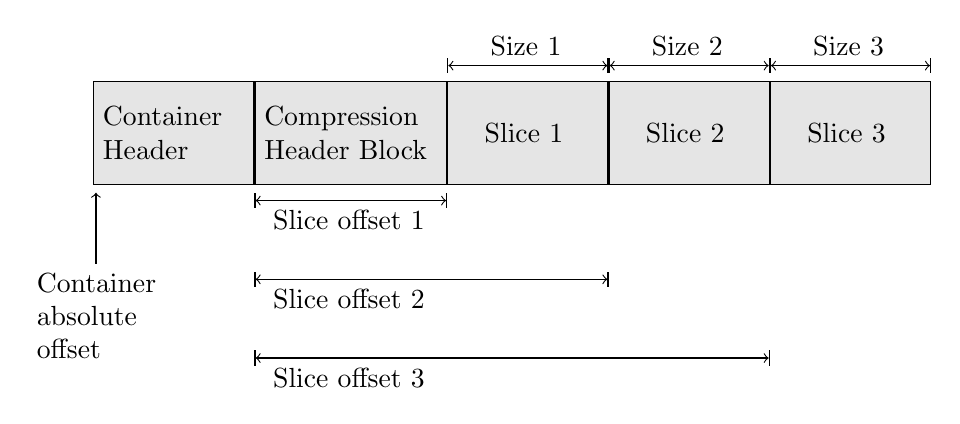
\begin{tikzpicture}[
  boxed/.style={rectangle, draw=black, fill=black!10, minimum height=1.3cm, text width=1.8cm},
]
\node(A) [boxed]{Container Header};
\node(B) [boxed,right,text width=2.2cm] at (A.east){Compression Header Block};
\node(C) [boxed,right] at (B.east){\quad Slice 1};
\node(D) [boxed,right] at (C.east){\quad Slice 2};
\node(E) [boxed,right] at (D.east){\quad Slice 3};

\draw[<-] (A.south west)+(1pt,-0.1cm) -- +(1pt,-1cm)
     node[below, text width=1.5cm]{Container absolute offset};


\draw[|<->|] ([yshift=-0.2cm]B.south west) node[below,xshift=1.2cm]{Slice offset 1}
    -- ([yshift=-0.2cm]B.south east);
\draw[|<->|] ([yshift=-1.2cm]B.south west) node[below,xshift=1.2cm]{Slice offset 2}
    -- ([yshift=-1.2cm]C.south east);
\draw[|<->|] ([yshift=-2.2cm]B.south west) node[below,xshift=1.2cm]{Slice offset 3}
    -- ([yshift=-2.2cm]D.south east);

\draw[|<->|] ([yshift=+0.2cm]C.north west) node[above,xshift=1cm]{Size 1} -- ([yshift=+0.2cm]C.north east);
\draw[|<->|] ([yshift=+0.2cm]D.north west) node[above,xshift=1cm]{Size 2} -- ([yshift=+0.2cm]D.north east);
\draw[|<->|] ([yshift=+0.2cm]E.north west) node[above,xshift=1cm]{Size 3} -- ([yshift=+0.2cm]E.north east);


\end{tikzpicture}
\end{center}

\subsubsection*{BAM index}

BAM indexes are supported by using 4-byte integer pointers called landmarks that 
are stored in container header. BAM index pointer is a 64-bit value with 48 bits 
reserved for the BAM block start position and 16 bits reserved for the in-block 
offset. When used to index CRAM files, the first 48 bits are used to store the 
CRAM container start position and the last 16 bits are used to store the index 
of the landmark in the landmark array stored in  container header. The landmark 
index can be used to access the appropriate slice. 

The above indexing scheme treats CRAM slices as individual records in BAM file. 
This allows to apply BAM indexing to CRAM files, however it introduces some overhead 
in seeking specific alignment start because all preceding records in the slice 
must be read and discarded.

\section{\textbf{Encodings}}
\label{sec:encodings}

% FIXME: we have a mishash of coding, encoding and codec.  We should
% go through the entire document and be consistent.

\subsection{\textbf{Introduction}}

The basic idea for codings is to efficiently represent some values in binary format. 
This can be achieved in a number of ways that most frequently involve some knowledge 
about the nature of the values being encoded, for example, distribution statistics. 
The methods for choosing the best encoding and determining its parameters are very 
diverse and are not part of the CRAM format specification, which only describes 
how the information needed to decode the values should be stored.

Note two of the encodings (Golomb and Golomb-Rice) are listed as deprecated.
These are still formally part of the CRAM specification, but have not been used by the primary implementations and may not be well supported.
Therefore their use is permitted, but not recommended.

\subsubsection*{Offset}

Many of the codings listed below encode positive integer numbers. An integer offset 
value is used to allow any integer numbers and not just positive ones to be encoded. 
It can also be used for monotonically decreasing distributions with the maximum 
not equal to zero. For example, given offset is 10 and the value to be encoded 
is 1, the actually encoded value would be offset+value=11. Then when decoding, 
the offset would be subtracted from the decoded value. 

\subsection{EXTERNAL: codec ID 1}

Can encode types \textit{Byte}, \textit{Integer}.

The EXTERNAL coding is simply storage of data verbatim to an external block with a given ID.
If the type is \textit{Byte} the data is stored as-is, otherwise for \textit{Integer} type the data is stored in ITF8.

\subsubsection*{Parameters}

CRAM format defines the following parameters of EXTERNAL coding: 

\begin{tabular}{|>{\raggedright}p{100pt}|>{\raggedright}p{100pt}|>{\raggedright}p{230pt}|}
\hline
\textbf{Data type} & \textbf{Name} & \textbf{Comment}
\tabularnewline
\hline
itf8 & external id & id of an external block containing the byte stream\tabularnewline
\hline
\end{tabular}

\subsection{Huffman coding: codec ID 3}

Can encode types \textit{Byte}, \textit{Integer}.

Huffman coding replaces symbols (values to encode) by binary codewords, with common symbols having shorter codewords such that the total message of binary codewords is shorter than using uniform binary codeword lengths.
The general process consists of the following steps.

\begin{itemize}
\item Obtain symbol code lengths.
\begin{itemize}
\item If encoding:\\
- Compute symbol frequencies.\\
- Compute code lengths from frequencies.
\item If decoding:\\
- Read code lengths from codec parameters.
\end{itemize}

\item Compute canonical Huffman codewords from code lengths\footnote{\url{https://en.wikipedia.org/wiki/Canonical_Huffman_code}}.

\item Encode or decode bits as per the symbol to codeword table.
Codewords have the ``prefix property'' that no codeword is a prefix of another codeword, enabling unambiguous decode bit by bit.
\end{itemize}

The use of canonical Huffman codes means that we only need to store the code lengths and use the same algorithm in both encoder and decoder to generate the codewords.
This is achieved by ensuring our symbol alphabet has a natural sort order and codewords are assigned in numerical order.

\textbf{Important note: for alphabets with only one value, the codeword will be zero bits long.}
This makes the Huffman codec an efficient mechanism for specifying constant values.

\subsubsection*{Canonical code computation}

\begin{enumerate}
\item Sort the alphabet ascending using bit-lengths and then using numerical order 
of the values.

\item The first symbol in the list gets assigned a codeword which is the same length 
as the symbol's original codeword but all zeros. This will often be a single zero 
('0').

\item Each subsequent symbol is assigned the next binary number in sequence, ensuring
that following codes are always higher in value.

\item When you reach a longer codeword, then after incrementing, append zeros until 
the length of the new codeword is equal to the length of the old codeword.
\end{enumerate}

\subsubsection*{Examples}

\begin{tabular}{|>{\raggedright}p{105pt}|>{\raggedright}p{105pt}|>{\raggedright}p{105pt}|}
\hline
\textbf{Symbol} & \textbf{Code length} & \textbf{Codeword}\tabularnewline
\hline
A & 1 & 0\tabularnewline
\hline
B & 3 & 100\tabularnewline
C & 3 & 101\tabularnewline
D & 3 & 110\tabularnewline
\hline
E & 4 & 1110\tabularnewline
F & 4 & 1111\tabularnewline
\hline
\end{tabular}

\subsubsection*{Parameters}

\begin{tabular}{|>{\raggedright}p{100pt}|>{\raggedright}p{100pt}|>{\raggedright}p{230pt}|}
\hline
\textbf{Data type} & \textbf{Name} & \textbf{Comment}
\tabularnewline
\hline
itf8[ ] & alphabet & list of all encoded symbols (values)\tabularnewline
\hline
itf8[ ] & bit-lengths & array of bit-lengths for each symbol in the alphabet\tabularnewline
\hline
\end{tabular}

\subsection{Byte array coding}

Often there is a need to encode an array of bytes where the length is not predetermined.
For example the read identifiers differ per alignment record, possibly with different lengths, and this length must be stored somewhere.
There are two choices available: storing the length explicitly (BYTE\_ARRAY\_LEN) or continuing to read bytes until a termination value is seen (BYTE\_ARRAY\_STOP).

Note in contrast to this, quality values are known to be the same length as the sequence which is an already known quantity, so this does not need to be encoded using the byte array codecs.

\subsubsection*{BYTE\_ARRAY\_LEN: codec ID 4}

Can encode types \textit{Byte[ ]}.

Byte arrays are captured length-first, meaning that the length of every array element is written using an additional encoding.
For example this could be a HUFFMAN encoding or another EXTERNAL block.
The length is decoded first followed by the data, followed by the next length and data, and so on.

This encoding can therefore be considered as a nested encoding, with each pair of nested encodings containing their own set of parameters.
The byte stream for parameters of the BYTE\_ARRAY\_LEN encoding is therefore the concatenation of the length and value encoding parameters as described in section~\ref{subsec:writing-bytes}.

The parameter for BYTE\_ARRAY\_LEN are listed below:

\begin{tabular}{|>{\raggedright}p{100pt}|>{\raggedright}p{100pt}|>{\raggedright}p{230pt}|}
\hline
\textbf{Data type} & \textbf{Name} & \textbf{Comment}
\tabularnewline
\hline
encoding\texttt{<}int\texttt{>} & lengths encoding & an encoding describing how 
the arrays lengths are captured\tabularnewline
\hline
encoding\texttt{<}byte\texttt{>} & values encoding & an encoding describing how 
the values are captured\tabularnewline
\hline
\end{tabular}

For example, the bytes specifying a BYTE\_ARRAY\_LEN encoding, including the codec and parameters, for a 16-bit X0 auxiliary tag (``X0C'') may use HUFFMAN encoding to specify the length (always 2 bytes) and an EXTERNAL encoding to store the value to an external block with ID 200.

\begin{tabular}{lll}
\hline
\textbf{Bytes} & & \textbf{Meaning}\\
\hline
\texttt{0x04}         & & BYTE\_ARRAY\_LEN codec ID                                    \\
\texttt{0x0a}         & & 10 remaining bytes of BYTE\_ARRAY\_LEN parameters            \\
\\
\texttt{0x03}         & & HUFFMAN codec ID, for aux tag lengths                        \\
\texttt{0x04}         & & 4 more bytes of HUFFMAN parameters                           \\
\texttt{0x01}         & & Alphabet array size = 1                                      \\
\texttt{0x02}         & & alphabet symbol; (length = 2)                                \\
\texttt{0x01}         & & Codeword array size = 1                                      \\
\texttt{0x00}         & & Code length = 0 (zero bits needed as alphabet is size 1)     \\
\\
\texttt{0x01}         & & EXTERNAL codec ID, for aux tag values                        \\
\texttt{0x02}         & & 2 more bytes of EXTERNAL parameters                          \\
\texttt{0x80 0xc8}    & & ITF8 encoding for block ID 200                               \\
\hline
\end{tabular}



\subsubsection*{BYTE\_ARRAY\_STOP: codec ID 5}

Can encode types \textit{Byte[ ]}.

Byte arrays are captured as a sequence of bytes terminated by a special stop byte.
The data returned does not include the stop byte itself.
In contrast to BYTE\_ARRAY\_LEN the value is always encoded with EXTERNAL so the parameter is an external id instead of another encoding.

\begin{tabular}{|>{\raggedright}p{100pt}|>{\raggedright}p{100pt}|>{\raggedright}p{230pt}|}
\hline
\textbf{Data type} & \textbf{Name} & \textbf{Comment}
\tabularnewline
\hline
byte & stop byte & a special byte treated as a delimiter\tabularnewline
\hline
itf8 & external id & id of an external block containing the byte stream\tabularnewline
\hline
\end{tabular}

\subsection{Beta coding: codec ID 6}

Can encode types \textit{Integer}.

\subsubsection*{Definition}

Beta coding is a most common way to represent numbers in \emph{binary notation} and is sometimes referred to as binary coding.
The decoder reads the specified fixed number of bits (most significant first) and subtracts the offset value to get the decoded integer.

\subsubsection*{Parameters}

CRAM format defines the following parameters of beta coding: 

\begin{tabular}{|>{\raggedright}p{144pt}|>{\raggedright}p{144pt}|>{\raggedright}p{144pt}|}
\hline
\textbf{Data type} & \textbf{Name} & \textbf{Comment}\tabularnewline
\hline
itf8 & offset & offset is subtracted from each value during decode\tabularnewline
\hline
itf8 & length & the number of bits used\tabularnewline
\hline
\end{tabular}

\subsubsection*{Examples}

If we have integer values in the range 10 to 15 inclusive, the largest value would traditionally need 4 bits, but with an offset of -10 we can hold values 0 to 5, using a fixed size of 3 bits.
Using fixed Offset and Length coming from the beta parameters, we decode these values as:

\begin{tabular}{|>{\raggedright}p{105pt}|>{\raggedright}p{105pt}|>{\raggedright}p{105pt}|>{\raggedright}p{105pt}|}
\hline
Offset & Length & \textbf{Bits} & \textbf{Value}\tabularnewline
\hline
-10 & 3 & 000 & 10\tabularnewline
\hline
-10 & 3 & 001 & 11\tabularnewline
\hline
-10 & 3 & 010 & 12\tabularnewline
\hline
-10 & 3 & 011 & 13\tabularnewline
\hline
-10 & 3 & 100 & 14\tabularnewline
\hline
-10 & 3 & 101 & 15\tabularnewline
\hline
\end{tabular}

\subsection{Subexponential coding: codec ID 7}

Can encode types \textit{Integer}.

\subsubsection*{Definition}

Subexponential coding\footnote{Fast progressive lossless image compression, Paul G. Howard and Jeffrey Scott Vitter, 1994. \url{http://www.ittc.ku.edu/~jsv/Papers/HoV94.progressive_FELICS.pdf}} is parametrized by a non-negative integer $k$.
For values $n < 2^{k+1}$ subexponential coding produces codewords identical to Rice coding \footnote{\url{https://en.wikipedia.org/wiki/Golomb_coding\#Rice_coding}}.  For larger values it grows logarithmically with $n$.

\subsubsection*{Encoding}

\begin{enumerate}
\item Add $\mathit{offset}$ to $n$.

\item Determine $u$ and $b$ values from $n$
\begin{align*}
b =
\begin{cases}
  \ k                        & \text{ if $n < 2^k$} \\
  \ \lfloor log_{2}n \rfloor & \text{ if $n \ge 2^k$}
\end{cases}
&\
&u =
\begin{cases}
  \ 0     & \text{ if $n < 2^k$} \\
  \ b-k+1 & \text{ if $n \ge 2^k$}
\end{cases}
\end{align*}

\item Write $u$ in unary form; $u$ 1 bits followed by a single 0 bit.

\item Write the bottom $b$-bits of $n$ in binary form.
\end{enumerate}

\subsubsection*{Decoding}

\begin{enumerate}
\item Read $u$ in unary form, counting the number of leading 1s (prefix) in the codeword (discard the trailing 0 bit).

\item Determine $n$ via:
\begin{enumerate}
\item if $u = 0$ then read $n$ as a $k$-bit binary number.
\item if $u \ge 1$ then read $x$ as a $(u + k - 1)$-bit binary. Let $n = 2^{u+k-1} + x$.
\end{enumerate}

\item Subtract $\mathit{offset}$ from $n$.
\end{enumerate}

\subsubsection*{Examples}

\begin{tabular}{|>{\raggedright}p{105pt}|>{\raggedright}p{105pt}|>{\raggedright}p{105pt}|>{\raggedright}p{105pt}|}
\hline
\textbf{Number} & \textbf{Codeword, k=0} & \textbf{Codeword, k=1} & \textbf{Codeword, 
k=2}\tabularnewline
\hline
0 & 0 & 00 & 000\tabularnewline
\hline
1 & 10 & 01 & 001\tabularnewline
\hline
2 & 1100 & 100 & 010\tabularnewline
\hline
3 & 1101 & 101 & 011\tabularnewline
\hline
4 & 111000 & 11000 & 1000\tabularnewline
\hline
5 & 111001 & 11001 & 1001\tabularnewline
\hline
6 & 111010 & 11010 & 1010\tabularnewline
\hline
7 & 111011 & 11011 & 1011\tabularnewline
\hline
8 & 11110000 & 1110000 & 110000\tabularnewline
\hline
9 & 11110001 & 1110001 & 110001\tabularnewline
\hline
10 & 11110010 & 1110010 & 110010\tabularnewline
\hline
\end{tabular}

\subsubsection*{Parameters}

\begin{tabular}{|>{\raggedright}p{100pt}|>{\raggedright}p{100pt}|>{\raggedright}p{230pt}|}
\hline
\textbf{Data type} & \textbf{Name} & \textbf{Comment}
\tabularnewline
\hline
itf8 & offset & offset is subtracted from each value during decode\tabularnewline
\hline
itf8 & k & the order of the subexponential coding\tabularnewline
\hline
\end{tabular}

\subsection{Gamma coding: codec ID 9}

Can encode types \textit{Integer}.

\subsubsection*{Definition}

\emph{Elias gamma code} is a prefix encoding of positive integers. This is a combination 
of unary coding and beta coding. The first is used to capture the number of bits 
required for beta coding to capture the value. 

\subsubsection*{Encoding}

\begin{enumerate}
\item Write it in binary.

\item Subtract $1$ from the number of bits written in step 1 and prepend that many zeros.

\item An equivalent way to express the same process:

\item Separate the integer into the highest power of $2$ it contains ($2N$) and the remaining 
$N$ binary digits of the integer.

\item Encode $N$ in unary; that is, as $N$ zeroes followed by a one.

\item Append the remaining $N$ binary digits to this representation of $N$.
\end{enumerate}

\subsubsection*{Decoding}

\begin{enumerate}
\item Read and count 0s from the stream until you reach the first 1. Call this count 
of zeroes $N$.

\item Considering the one that was reached to be the first digit of the integer, with 
a value of $2N$, read the remaining $N$ digits of the integer.
\end{enumerate}

\subsubsection*{Examples}

\begin{tabular}{|>{\raggedright}p{76pt}|>{\raggedright}p{107pt}|}
\hline
\textbf{Value} & \textbf{Codeword}\tabularnewline
\hline
1 & 1\tabularnewline
\hline
2 & 010\tabularnewline
\hline
3 & 011\tabularnewline
\hline
4 & 00100\tabularnewline
\hline
\end{tabular}

\subsubsection*{Parameters}

\begin{tabular}{|>{\raggedright}p{144pt}|>{\raggedright}p{144pt}|>{\raggedright}p{144pt}|}
\hline
\textbf{Data type} & \textbf{Name} & \textbf{Comment}\tabularnewline
\hline
itf8 & offset & offset to subtract from each value after decode\tabularnewline
\hline
\end{tabular}

\subsection{DEPRECATED: Golomb coding: codec ID 2}

Can encode types \textit{Integer}.

Note this codec has not been used in any known CRAM implementation since before CRAM v1.0.
Nor is it implemented in some of the major software.
Therefore its use is not recommended.

\subsubsection*{Definition}

\emph{Golomb encoding} is a prefix encoding optimal for representation of random 
positive numbers following geometric distribution. 

\subsubsection*{Encoding}

\begin{enumerate}
\item Fix the parameter $M$ to an integer value.

\item For $N$, the number to be encoded, find

\begin{enumerate}
\item quotient $q = \lfloor N/M \rfloor$

\item remainder $r = N \bmod M$
\end{enumerate}

\item Generate Codeword

\begin{enumerate}
\item The Code format : \texttt{<}Quotient Code\texttt{>}\texttt{<}Remainder Code\texttt{>}, 
where

\item Quotient Code (in unary coding)

\begin{enumerate}
\item Write a $q$-length string of 1 bits

\item Write a 0 bit
\end{enumerate}

\item Remainder Code (in truncated binary encoding)

Set $b=\lceil log_{2}(M) \rceil$

\begin{enumerate}
\item If $r < 2^{b}-M$ code $r$ as plain binary using $b-1$ bits.

\item If $r \ge 2^{b}-M$ code the number $r+2^{b}-M$ in plain binary representation 
using $b$ bits.
\end{enumerate}
\end{enumerate}
\end{enumerate}

\subsubsection*{Decoding}

\begin{enumerate}
\item Read $q$ via unary coding: count the number of 1 bits and consume the following 0 bits.
\item Set $b=\lceil log_{2}(M) \rceil$
\item Read $r$ via $b-1$ bits of binary coding
\item If $r \ge 2^{b}-M$
\begin{enumerate}
\item Read 1 single bit, $x$.
\item Set $r = r*2 + x - (2^{b}-M)$
\end{enumerate}
\item Value is $q*M + r - \mathit{offset}$
\end{enumerate}

\subsubsection*{Examples}

\begin{tabular}{|>{\raggedright}p{76pt}|>{\raggedright}p{107pt}|}
\hline
\textbf{Number} & \textbf{Codeword, M=10, (thus b=4)}\tabularnewline
\hline
0 & 0000\tabularnewline
\hline
4 & 0100\tabularnewline
\hline
10 & 10000\tabularnewline
\hline
26 & 1101100\tabularnewline
\hline
42 & 11110010\tabularnewline
\hline
\end{tabular}

\subsubsection*{Parameters}

Golomb coding takes the following parameters: 

\begin{tabular}{|>{\raggedright}p{144pt}|>{\raggedright}p{144pt}|>{\raggedright}p{144pt}|}
\hline
\textbf{Data type} & \textbf{Name} & \textbf{Comment}\tabularnewline
\hline
itf8 & offset & offset is added to each value\tabularnewline
\hline
itf8 & M & the golomb parameter (number of bins)\tabularnewline
\hline
\end{tabular}

\subsection{DEPRECATED: Golomb-Rice coding: codec ID 8}

Can encode types \textit{Integer}.

Note this codec has not been used in any known CRAM implementation since before CRAM v1.0.
Nor is it implemented in some of the major software.
Therefore its use is not recommended.

Golomb-Rice coding is a special case of Golomb coding when the M parameter is a power of 2.
The reason for this coding is that the division operations in Golomb coding can be replaced with bit shift operators as well as avoiding the extra $r < 2^{b}-M$ check.

\section{\textbf{External compression methods}}

External encoding operates on bytes only. Therefore any data series must be translated into bytes before sending data into an external block.
The following methods are defined.
Exact definitions of these methods are in their respective internet links or the ancillary \textit{CRAMcodecs} document found along side this specification.

Integer values are written as ITF8, which then can be translated into an array 
of bytes. 

Strings, like read name, are translated into bytes according to UTF8 rules. In 
most cases these should coincide with ASCII, making the translation trivial.

Each method has an associated numeric code which is defined in Section~\ref{sec:block-struct}.

\subsection{\textbf{Gzip}}

The Gzip specification is defined in RFC 1952.
Gzip in turn is an encapsulation on the Deflate algorithm defined in RFC 1951.

\subsection{\textbf{Bzip2}}

First available in CRAM v2.0.

Bzip2 is a compression method utilising the Burrows Wheeler Transform, Move To Front transform, Run Length Encoding and a Huffman entropy encoder. 
It is often superior to Gzip for textual data.

An informal format specification exists:\\
\url{https://github.com/dsnet/compress/blob/master/doc/bzip2-format.pdf}

\subsection{\textbf{LZMA}}

First available in CRAM v3.0.

LZMA is the Lempel-Ziv Markov chain algorithm.
CRAM uses the xz Stream format to encapsulate this algorithm, as defined in \url{https://tukaani.org/xz/xz-file-format.txt}.

\subsection{\textbf{rANS4x8 codec}}

First available in CRAM v3.0.

rANS is the range-coder variant of the Asymmetric Numerical
System\footnote{J. Duda, \textit{Asymmetric numeral systems: entropy
    coding combining speed of Huffman coding with compression rate of
    arithmetic coding}, \url{http://arxiv.org/abs/1311.2540}}.

``4x8'' refers to 4-way interleaving with 8-bit renormalisation.\newline
This variant of rANS first appeared in CRAM v3.0.

Details of this algorithm have been moved to the \textit{CRAMcodecs} document.

\subsection{\textbf{rANS4x16 codec}}

First available in CRAM v3.1.

``4x16'' refers to 4-way interleaving with 16-bit renormalisation.\newline
This variant of rANS first appeared in CRAM v3.1.

Details of this algorithm are listed in the \textit{CRAMcodecs} document.

\subsection{\textbf{adaptive arithemtic coding}}

First available in CRAM v3.1.

An entropy encoder that is slower but slightly more concise than
rANS.  It achieves this by adapting the probabilities as it compresses
and decompresses instead of using a fixed table.

Details of this algorithm are listed in the \textit{CRAMcodecs} document.

\subsection{\textbf{fqzcomp codec}}

First available in CRAM v3.1.

This is a method dedicated to compression of quality values.

Details of this algorithm are listed in the \textit{CRAMcodecs} document.

\subsection{\textbf{name tokeniser}}

First available in CRAM v3.1.

This is a method dedicated to compression of read names.

Details of this algorithm are listed in the \textit{CRAMcodecs} document.

\section{\textbf{Appendix}}
\subsection{\textbf{Choosing the container size}}

CRAM format does not constrain the size of the containers. However, the following 
should be considered when deciding the container size:

$\bullet$ Data can be compressed better by using larger containers

$\bullet$ Random access performance is better for smaller containers 

$\bullet$ Streaming is more convenient for small containers

$\bullet$ Applications typically buffer containers into memory

We recommend 1 megabyte containers. They are small enough to provide good random access
and streaming performance while being large enough to provide good compression. 
1\MB\ containers are also small enough to fit into the L2 cache of most modern CPUs.

Some simplified examples are provided below to fit data into 1\MB\ containers.

\textbf{Unmapped short reads with bases, read names, recalibrated and original 
quality scores}

We have 10,000 unmapped short reads (100bp) with read names, recalibrated and original 
quality scores. We estimate 0.4 bits/base (read names) + 0.4 bits/base (bases) 
+ 3 bits/base (recalibrated quality scores) + 3 bits/base (original quality scores) 
$\approx$ 7 bits/base. Space estimate is $10\,000 \times 100 \times 7 \bits
\approx 0.9 \MB$. Data could be stored in a single container.

\textbf{Unmapped long reads with bases, read names and quality scores}

We have 10,000 unmapped long reads (10kb) with read names and quality scores. We 
estimate: 0.4 bits/base (bases) + 3 bits/base (original quality scores) $\approx$
3.5 bits/base. Space estimate is $10\,000 \times 10\,000 \times 3.5 \bits
\approx 42 \MB$. Data could be stored in $42 \times 1\MB$ containers.

\textbf{Mapped short reads with bases, pairing and mapping information}

We have 250,000 mapped short reads (100bp) with bases, pairing and mapping information. 
We estimate the compression to be 0.2 bits/base. Space estimate is $250\,000 \times 100
\times 0.2 \bits \approx 0.6 \MB$. Data could be stored in a single
container.

\textbf{Embedded reference sequences}

We have a reference sequence (10Mb). We estimate the compression to be 2 bits/base. 
Space estimate is $10\,000\,000 \times 2 \bits \approx 2.4 \MB$. Data
could be written into three containers: $1\MB + 1\MB + 0.4\MB$.

\newpage

\subsection{CRAM History}

\subsubsection*{Pre-CRAM: 2010}

The primary concepts and ideas of CRAM stem from work at the European
Bioinformatics Institute in 2010 and 2011, published in:

\begin{quote}\small
Markus Hsi-Yang Fritz,
Rasko Leinonen, Guy Cochrane, and Ewan Birney,
\textbf{Efficient storage of high throughput DNA sequencing data using reference-based compression},
{\sl Genome Res.}~2011~21: 734--740;
\href{http://dx.doi.org/doi:10.1101/gr.114819.110}{doi:10.1101/gr.114819.110};
{\sc pmid:}21245279.
\end{quote}

\subsubsection*{CRAM 0.x: 2011}

Vadim Zalunin implemented the ideas in the paper, now named CRAM, in
the Java CRAMtools package.  This included versions from 0.3 to 0.86\footnote{\url{https://github.com/vadimzalunin/crammer/releases}}.

\subsubsection*{CRAM 1.0: 2012}

The first official launch of the CRAM specification, in the Java
CRAMtools package\footnote{\url{https://github.com/enasequence/cramtools}}

This was publicised at \url{https://github.com/enasequence/cramtools}.

\subsubsection*{CRAM 2.0: 2013}

Reimplementing CRAM in C
\footnote{Staden IO\_Lib 1.13.0 and later HTSlib 0.2.0} exposed a number of issues with the
1.0 specification and disparities between the specification text and
the Java implementation.  CRAM 2.0 unified implementation with
specification.

Other changes included:

\begin{itemize}
\item Support for multiple references per container, to permit storage
of highly fragmented assemblies.

\item Soft-clips and inserted bases moved to their own separate
data-series instead of sharing one.

\item Slice headers contain meta-data tracking the number of records
and bases.

\item Corrected the BF (bam flag) data series to match the BAM
specification.

\item Improved encoding of auxiliary tags.
\end{itemize}

\subsubsection*{CRAM 2.1: 2014}

This is the first version to appear in HTSJDK (version 1.127), ported
from the Java CRAMtools package.

\begin{itemize}
\item EOF blocks are added in order to spot truncated files.
\end{itemize}

\subsubsection*{CRAM 3.0: 2014}

Primarily this is an optimisation of size and speed.

\begin{itemize}
\item Inclusion of LZMA compression library.
\item Inclusion of the custom rANS Order-0 and Order-1 entropy encoders.
\item Checksums added to all file format structures to ensure data integrity.
\end{itemize}

\subsubsection*{CRAM 3.1: 2023}

Note: the formal draft appeared in 2019, and was initially
demonstrated in 2016.

This adds new EXTERNAL compression methods, described in the separate
CRAMcodecs document, and expands the list of permitted ``methods'' in
the CRAM Block structure.

The aim of the new compression methods is improved compression, both
performance with the newer SIMD rANS implementation and file size with
custom name tokeniser and quality codec.

The format is otherwise identical to 3.0.

\newpage

\subsection{\textbf{Contributors and Acknowledgements}}

\begin{itemize}
\item
Markus Fritz, Rasko Leinonen, Guy Cochrane and Ewan Birney (EBI):
Initial ideas behind CRAM.

\item Vadim Zalunin (EBI):
Initial JAVA implementation of CRAM and previous maintainer of CRAM specification.

\item James Bonfield (Sanger Institute):
Initial C implementation of CRAM and current maintainer of CRAM
specification.

\item Joel Thibault (Broad Institute):
previous maintainer of CRAM specification.

\item Chris Norman (Broad Institute):
previous maintainer of CRAM specification and worked on
the HTSJDK implementation.

\item Robert Buels (UC Berkeley): First JavaScript implementation of CRAM

\item Michael Macias (St Jude Children's Research Hospital): First Rust implementation of CRAM

\item Other specification contributors include: John Marshall, Rishi Nag,
Kenta Sato, Artem Tarasov and Jason Travis.

\item Plus a big thank you to everyone who has raised GitHub issues
and/or helped us improve the specification in other ways.
\end{itemize}

\end{document}
